\documentclass[11pt]{article}

\usepackage{smoothing_paper}


\usepackage[section]{placeins}

%%%%%%%%%%%%%%%%%%%%%%%%%%%%%%%%chiheb commands

\newcommand{\ie}{\emph{i.e.}}
\newcommand{\eg}{\emph{e.g.}}
\newcommand{\cf}{\emph{cf.}}
\newcommand{\prob}[1]{\mathrm{P}\left(#1\right)}
\newcommand{\expt}[1]{\mathrm{E}\left[#1\right]}
\newcommand{\expth}[1]{\hat{\mathrm{E}}\left[#1\right]}



\newcommand{\rset}{\mathbb{R}}
\newcommand{\nset}{\mathbb{N}}
\newcommand{\zset}{\mathbb{Z}}



\newcommand{\PERIOD}{.}
\newcommand{\COMMA}{,}
\newcommand{\BIGSPACE}{\,\,\,\,\,\,\,}



\newcommand{\Ordo}[1]{{\mathcal{O}}\left(#1\right)}
\newcommand{\ordo}[1]{{o}\left(#1\right)}

%%%%%%%%%%%%%%%%%%%%%%%%%%%%%%%%%%%%%%%%%%%%%%%%%%%%%%%%%%%%%%%%%%%%%%%%
%%
%% DO WE RELLY NEED THE FOLLOWING??

%%  new margin
%%%%%%%%%%%%%%%%%%%%%%%%%%%%%%%%%%%%%%%%%%%
\pagestyle{plain}                                                      %%
%%%%%%%%%% EXACT 1in MARGINS %%%%%%%                                   %%
\setlength{\textwidth}{6.5in}     %%                                   %%
\setlength{\oddsidemargin}{0in}   %%   
\setlength{\evensidemargin}{0in}  %%        
\setlength{\textheight}{8.5in}    %%       
\setlength{\topmargin}{-0.2in}    %%   
\setlength{\headheight}{0in}      %%    
\setlength{\headsep}{0in}         %%                   
\setlength{\footskip}{.5in}       %%                       
%%%%%%%%%%%%%%%%%%%%%%%%%%%%%%%%%%%%                                   %%
\newcommand{\required}[1]{\section*{\hfil #1\hfil}}                    %%
\renewcommand{\refname}{\hfil References Cited\hfil}                   %%

\def\SMALLSKIP{\smallskip}
\def\MEDSKIP{\medskip}
\def\BIGSKIP{\bigskip}

%%
%%%%%%%%%%%%%%%%%%%%%%%%%%%%%%%%%%%%%%%%%%%%%%%%%%%%%%%%%%%%%%%%%%%%%

\makeatletter
\def\BState{\State\hskip-\ALG@thistlm}
\makeatother



%%%%%%%%%%%%%%%%%%%%%%%%%%%%%%%%%%%%%%%%

\title{Efficient option pricing for Rough Bergomi model} 
    \date{ }

\begin{document}
\maketitle

\section{Introduction}
\subsection{The goal and outline of the project}
The main goal of the project is to design a fast option pricer, based on multi-index stochastic collocation (MISC) as \cite{haji2016multi}, for options whose dynamics follow rBergomi model as in \cite{bayer2016pricing}. We may later investigate QMC.

\subsection{Review of literature}
Extending the Black-Scholes model, in which volatility is assumed to be constant, to the case where the volatility is stochastic has proved to be successful in explaining certain phenomena observed in option price data, in particular the implied volatility smile. The main drawback of such stochastic volatility models, however, is that they are unable to capture the true steepness of the implied volatility smile close to maturity. 
While choosing to add jumps to stock price models, for example modelling the stock price process as an exponential L\'evy process, does indeed produce steeper implied volatility smiles, the issue of the presence of jumps in stock price processes remains controversial\cite{bajgrowicz2015jumps,christensen2014fact}.

As an alternative to diffusive stochastic volatility models, rough stochastic volatility has emerged as a new paradigm in quantitative finance,  motivated by the statistical analysis of realised volatility by Gatheral, Jaisson and Rosenbaum \cite{gatheral2014volatility} and the theoretical results on implied volatility by Fukasawa \cite{fukasawa2011asymptotic}. In these models, the trajectories of volatility are less regular than those of the standard Brownian motion. As shown in \cite{gatheral2014volatility,bayer2016pricing}, these models are a family of (continuous-path) stochastic volatility models where the driving noise of the volatility process has H\"older regularity lower than Brownian motion, typically achieved by modeling the fundamental noise innovations of the volatility process as a fractional Brownian motion with Hurst exponent (and hence H\"older regularity)$0<H<1/2$.   A major advantage of such rough volatility models is the fact that they allow to  explain crucial phenomena  observed in  financial markets both from a statistical \cite{gatheral2014volatility,bennedsen2016decoupling} and
an option-pricing point of view \cite{bayer2016pricing}. For instance, it was observed empirically  that in equity markets   that as time to maturity becomes small the empirical implied volatility skew follows a power law with negative exponent, and thus becomes arbitrarily large near zero.  While standard stochastic volatility models with continuous paths struggle to capture this phenomenon, predicting instead a constant at-the-money implied volatility behaviour on he short end  \cite{gatheral2011volatility}, 
 fractional stochastic volatility models (and more specifically so-called rough volatility models) constitute  alternative  models  that  fit empirical implied volatilities for short dated options. Consequently, they have become the go-to models capable of reproducing stylised facts of financial markets.



 Rough volatility models are based on fractional Brownian motion (fBM), which  is a centred Gaussian process, whose covariance structure depends on the Hurst parameter $H \in (0, 1)$. If $H \in(0,1/2)$, then the fractional Brownian motion has negatively correlated increments and "rough" sample paths, and if $H \in (1/2,1)$ then it has positively correlated increments and "smooth" sample paths, when compared with a standard Brownian motion, which is recovered by taking $H=1/2$. Gatheral, Jaisson, and Rosenbaum \cite{gatheral2014volatility} justify  empirically  the benefits of such models; in particular, they argue that log-volatility in practice behaves essentially as fBM with the Hurst exponent $H \approx 0.1$ at any reasonable time scale (see also  \cite{gatheral2014volatility_2}). This finding is confirmed  by Bennedsen, Lunde and Pakkanen \cite{bennedsen2016decoupling}, who study over a thousand individual US equities and find that the Hurst parameter $H$ lies in $(0,1/2)$ for each equity.




 The rough Bergomi (rBergomi) model is one of the recent rough volatility models, developed by Bayer, Friz and Gatheral \cite{bayer2016pricing},  that is consistent with the stylised fact of implied volatility surfaces being essentially time-invariant, and are able to capture the term structure of skew observed in equity markets. In \cite{bayer2016pricing}, the authors constructed the rBergomi model by  moving from  physical to pricing measure and simulated prices under that model to fit well the implied volatility surface in the case of the S\&P $500$ index with
 few parameters-just three!. They claim that the fractional model generates strong skews or "smiles" in the implied volatility even for very short time to maturity so that this modeling provides an
 alternative to using jumps to model such an effect. In \cite{bayer2016pricing} the model is so named because of its relationship with the Bergomi variance curve model \cite{bergomi2005smile}, and may be seen as a non-Markovian
generalisation of the latter.


%From a practical perspective  a natural issue  appears: What does the mantra of rough volatility mean for a trader with a view to hedging his positions?


 Due to the non-Markovian nature of the fractional driver, pricing  and hedging under rough volatility constitute a significant challenge. In fact, the popularity of asset pricing models hinges on the availability of efficient numerical pricing methods. In the case of diffusions, these include Monte Carlo (MC) estimators, PDE discretization schemes, asymptotic expansions and transform
methods. With fractional Brownian motion being the prime example of a process beyond the semi-martingale framework, most currently prevalent option pricing methods -particularly the ones assuming semimartingality or Markovianity - may not easily carry over to the rough setting. In fact,  due to the lack of Markovianity or affine structure, conventional analytical pricing methods  do not apply. At the moment, the only known method for pricing  options under such models is MC simulation. In particular, recent advances in simulation methods for the rough Bergomi model have been achieved in \cite{bayer2016pricing,bayer2017regularity,mccrickerd2017turbocharging,bennedsen2017hybrid,jacquier2018vix}. For isntance, in \cite{mccrickerd2017turbocharging}, the authors employ a novel composition of variance reduction methods, immediately applicable to any conditionally log-normal  stochastic volatility model. They got a substatantial computation gain in the pricing  over the exisiting MC methods. On the other hand,  more analytical results of option pricing and implied volatility under this model has been done in \cite{jacquier2017pathwise,bayer2017short,forde2017asymptotics}. For isntance, in \cite{jacquier2017pathwise},
they  characterise the small-time behaviour of implied volatility using large deviations theory and  related results, concerning the small-time near-the-money skew, have been  obtained by Bayer, Friz, Gulisashvili, Horvath and Stemper \cite{bayer2017short}. However, we should point out that pricing and model calibration under rough volatility models still remains time consuming.


In this paper, we suggest to design  a fast option pricer, based on multi-index stochastic collocation (MISC) as in \cite{haji2016multi}, for options whose dynamics follow rBergomi model as in \cite{bayer2016pricing}. We may later investigate QMC.



%Following \cite{gatheral2014volatility}, Bayer, Friz and Gatheral \cite{bayer2016pricing} propose the so-called rough Bergomi model, which they then use to price options on integrated volatility and on the underlying itself. The advantage of their model is that it captures the "rough" behaviour of log volatility, in accordance with \cite{bennedsen2016decoupling,gatheral2014volatility}, as well
%as fits observed implied volatility smiles better than traditional Markovian stochastic volatility models, most notably in the close-to-maturity case.

%It is a well-documented fact on Equity markets (see for instance  Chapter 5 of \cite{gatheral2011volatility}) that standard (It\^o) stochastic models with continuous paths are not able to capture the observed steepness of the left wing of the smile when the maturity becomes small. To remedy this, several authors have
%suggested the addition of jumps, either in the form of an independent L\'evy process or within the more general
%framework of affine diffusions. Jumps (in the stock price dynamics) imply an explosive behaviour for the small maturity
%smile and are better able to capture the observed steepness of the small-maturity implied volatility smile. In particular, Tankov \cite{tankov2011pricing} showed that, for exponential L\'evy models with L´evy measure supported on the whole real line, the squared implied volatility smile explodes as $\sigma^2_\tau(k)\sim −k^2/(2\tau\log\tau)$, as the maturity tends to zero, where $k$ represents the log-moneyness. Such a small-maturity behaviour of the smile is not only captured by jump-based models, but rough volatility (non-Markovian) models, where the stochastic volatility
%component is driven by a fractional Brownian motion, are in fact also able to reflect this property of the data.
 
% Indeed both regimes have been identified from the empirical perspective. We refer to for instance \cite{gatheral2014volatility}
% for observations of rough volatility, while in \cite{chronopoulou2012estimation}  of volatility with long-range correlation properties are reported. Long-range volatility
% situations have been reported for currencies in \cite{walther2017true} and  for commodities
% in \cite{charfeddine2014true}, while analysis of
% electricity markets data typically gives $H<1/2$ as in \cite{rypdal2013modeling,bennedsen2015rough}. We believe that both the rough and the long range cases are important and can be observed depending on the specific market and regime.

% In a series of papers several authors \cite{bayer2017short,forde2017asymptotics,jacquier2017pathwise}  have indeed proved that, when the Hurst index of the fractional Brownian motion lies within $(0,1/2)$, then the implied volatility explodes at a rate of $\tau^{H-1/2}$ as the maturity tends to zero.
\subsection{Background on Gaussian and fBM processes}
A zero-mean real-valued Gaussian process $(Z_t)_{t\ge0}$ is a stochastic process such that on any finite subset $\{t_1,\dots t_n\} \subset \rset, (Z_{t_1},\dots, Z_{t_n})$ has a
multivariate normal distribution with mean zero. The law of a Gaussian process is entirely determined by the covariance function $K(s, t)= \expt{Z_t Z_s}$ and $Z$ induces a Gaussian probability
measure on $(E, \mathcal{B}(E))$, where $E$ denotes the Banach space $C_0([0,1])$ with the usual sup norm topology (see, e.g., section 3.1.1 of  \cite{carmona2007interest} for details).



Fractional Brownian motion (fBM) is a natural generalization of standard Brownian motion which preserves the properties of stationary increments, self-similarity, and Gaussian finite-dimensional distributions, but it has a more complex dependence structure. In this section, we recall the definition and summarize the basic properties of fBM.

A zero-mean Gaussian process $B^H_t$ is called standard fractional Brownian motion (fBM) with Hurst parameter $H \in(0,1)$ if it has covariance function

\begin{align}\label{eq:fbm_cov}
R_H=\expt{B_t^H B_s^H}-\expt{B_t^H}\expt{B_s^H}=\frac{1}{2} \left(\abs{t}^{2H}+\abs{s}^{2H}-\abs{t-s}^{2H}\right).	
\end{align}



In order to specify the distribution of a Gaussian process, it is enough to specify its mean and its covariance function; therefore, for each $H$, the law of $B^H$ is uniquely determined by $R_H(s, t)$. However, this definition by itself does not guarantee the existence of fBM; to show that fBM exists, one needs to verify that the covariance function is nonnegative definite.

We now recall some fundamental properties of fBM (see also Figure \ref{fig:fBM}):

\begin{itemize}
	\item fBM is continuous a.s. and H-self-similar (H-ss), i.e., for $a>0, (B_{at})_{t \ge 0}  \overset{(d)}{=} a^H (B_t)_{t \ge 0}$ where $ \overset{(d)}{=}$ means both processes have the same finite-dimensional distributions. For $H \neq 1/2$, $B^H$ does not have independent increments; for $H=1/2, B^H_t$ is the standard Brownian motion. 
	\item From \eqref{eq:fbm_cov}, we see that 
	\begin{equation*}
	\expt{(B_t^H-B_s^H)^2}=\abs{t-s}^{2H},
	\end{equation*}
so $B_t^H-B_s^H \sim \mathcal{N}(0,\abs{t-s}^{2H})$; thus $B^H$ has stationary increments.
\item If we set $X_n=B^H_n-B^H_{n-1}$, then $X_n$ is a  discrete-time Gaussian process with covariance function

\begin{align*}
\rho_n&=\expt{X_{k+n} X_n}=\expt{\left(B_{k+n}^H -B^H_{k+n-1}\right)\left(B_{k}^H -B^H_{k-1}\right)}\\
&\sim H (2H-1) n^{2H-2}\quad (n \rightarrow \infty),
\end{align*}
and thus (by convexity of the function $g(n) = n^{2H})$, we see that two increments the form $B_k-B_{k-1}$ and $B_{k+n}-B_{k+n-1}$ are positively correlated if $H  \in (1/2,1)$ and negatively correlated if $H \in (0,1/2)$. Thus $B^H$ is persistent (i.e., it is more likely to keep a trend than to break it) when $H>1/2$, the relatively stronger positive correlation for the consecutive increments of the associated fBm process with increasing $H$ values gives a relatively smoother process whose correlations decay relatively slowly.On the other hand, it is antipersistent when $H<1/2$ (i.e., if $B^H$ was increasing in the past, it is more likely to decrease in the future, and vice versa). The enhanced negative correlation with smaller Hurst exponent gives a relatively rougher process.

\item If $H \in (1/2,1)$, we can show that $\sum_{n=1}^\infty \rho_n= \infty$, which means that the process exhibits long-range dependence, but if $H \in(0, 1/2)$, then  $\sum_{n=1}^\infty \rho_n< \infty$.

\item Using that $\expt{(B^H_t- B^H_s)^2} = (t-s)^{2H}$, we can show that sample paths of $B^H$ are $\alpha$-H\:older continuous for all $\alpha \in (0,H)$.
\item fBM is the only self-similar Gaussian process with stationary increments (see, e.g., \cite{marquardt2006fractional}), and for $H\neq 1/2$, $B^H_t$ is neither a Markov process nor a semimartingale (see, e.g., \cite{nualart2006malliavin}).
\end{itemize}



For more details regarding the fBm processes we refer to \cite{biagini2008stochastic,coutin07introduction,mandelbrot1968fractional}.

\begin{figure}[h!]
	\centering
	\begin{subfigure}{.45\textwidth}
		\centering
		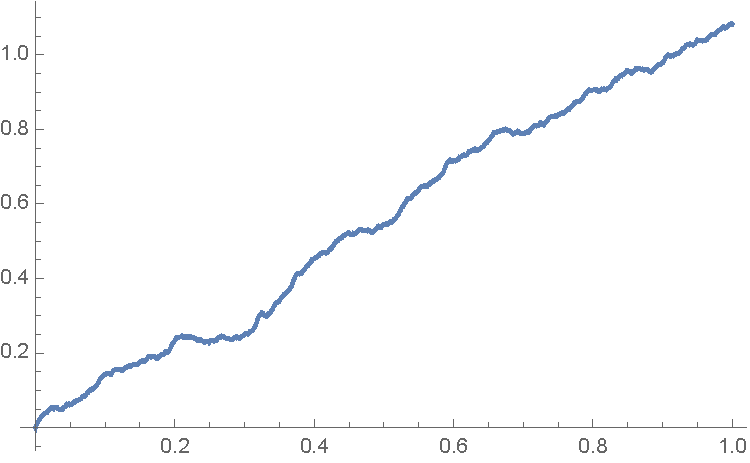
\includegraphics[width=1\linewidth]{./figures/fbm_H_0_9}
		\caption{}
		\label{fig:sub3}
	\end{subfigure}%
	\begin{subfigure}{.45\textwidth}
		\centering
		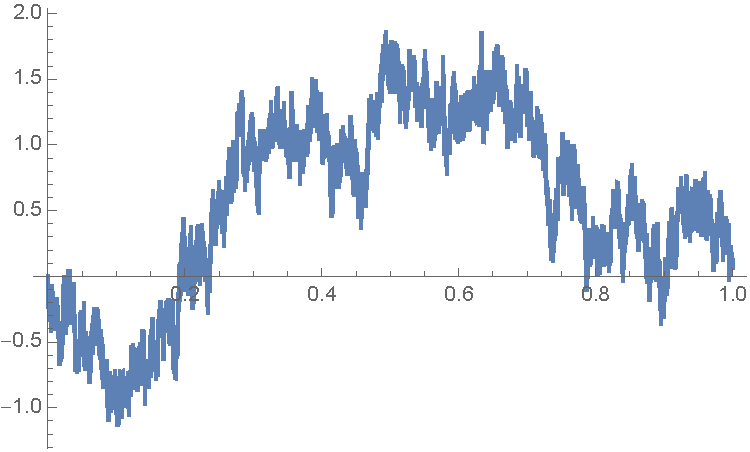
\includegraphics[width=1\linewidth]{./figures/fbm_H_0_3}
		\caption{}
		\label{fig:sub4}
	\end{subfigure}
	\caption{Monte Carlo simulation of fBM for $H = 0.9$ (left) and $H = 0.3$ (right).}
	\label{fig:fBM}
\end{figure}



\section{Problem setting}
\subsection{The rBergomi model}\label{sec:The rBergomi model}

We use  the rBergomi model for the price process $S_t$ as defined in  \cite{bayer2016pricing}, normalized to $r=0$, which is defined by

\begin{align}\label{eq:rBergomi_model1}
	dS_t = \sqrt{v_t(\tilde{W}^H)} S_t dZ_t,\\
	v_t = \xi_0(t) \exp\left( \eta \tilde{W}_t^H - \frac{1}{2} \eta^2 t^{2H} \right),
\end{align}
where for $0 < H < 1$ and  $\eta>0$.  We have $\tilde{W}^H $ is a certain Volterra process (Riemann-Liouville
process),  defined by
\begin{align}\label{eq:Volterra process}
	\tilde{W}_t^H = \int_0^t K^H(t,s) dW_s^1, \quad t \ge 0
\end{align}
where the kernel $K^H : \rset_+ \times \rset_+ \rightarrow \rset_+$ reads
\begin{align}
 \quad K^H(t,s) = \sqrt{2H} (t-s)^{H - 1/2},\quad \forall \: 0 \le s \le t.
\end{align}

We note that the map $s \rightarrow K^H(s,t)$ belongs to $L^2$, so
that the stochastic integral \eqref{eq:Volterra process} is well defined.

$W^1, Z$ denote two \emph{correlated} standard Brownian motions with correlation $\rho \in [-1,1]$, so that
\begin{align}
	Z:=\rho	W^1+ \bar{\rho}W^\perp \equiv \rho W^1+\sqrt{1-\rho^2} W^\perp,
\end{align}
where $(W^1,W^\perp)$ are two independent standard Brownian motions,
Therefore, Eq \ref{eq:rBergomi_model1} can be written as 

\begin{align}\label{eq:rBergomi_model}
	S_t&= S_0  \operatorname{exp}\left( \int_{0}^{t} \sqrt{v(s)} dZ(s)- \frac{1}{2} \int_{0}^{t} v(s) ds   \right),\quad S_0>0 \nonumber\\
	v(u)&=\xi_0(u) \operatorname{exp}\left( \eta \tilde{W}_u^H- \frac{\eta^2}{2} u^H \right), \quad \xi_0>0
\end{align}


The filtration $(\mathcal{F}_t)_{t\ge 0}$ can here be taken as the one generated by the two-dimensional Brownian motion $(W^1,W^\perp)$ under the risk neutral measure $\mathbb{Q}$, resulting in  a filtered probability space $(\Omega,\mathcal{F}; \mathcal{F}_t,\mathbb{Q})$. The stock price process $S$ is clearly then a local
$(\mathcal{F}_t)_{t\ge 0}$-martingale and a supermartingale, therefore integrable.  We shall henceforth use the notation $\expt{.} = E^{\mathbb{Q}}\left[. \mid \mathcal{F}_0\right]$ unless we state otherwise.

We refer to $v_u$ as the variance process, where $\xi_0(u) = \expt{v_u} \in \mathcal{F}_0$ a.s. the forward variance curve. $\tilde{W}^H $ is a centered, locally $(H-\epsilon)$- H\" \o lder continuous, Gaussian process with $\var{[\tilde{W}^H_t]} = t^{2H}$.




We note that the model parameters $(\eta,\rho,H)$ may have an
 intuitive interpretation of their influence over implied volatilities. In fact,   $\eta$ might seen as  smile, $\rho$ as skew, $H-1/2$ as the explosion(smile and skew).

\subsection{Option pricing under rBergomi model}\label{sec:Option pricing under rBergomi model}

Assuming $S_0 = 1$, and using the conditioning argument on the $\sigma$-algebra generated by $W^1$ (argument first used by \cite{romano1997contingent} in the context of Markovian SV
models), we can  show that the call price is given by

\begin{align}\label{BS_formula_rbergomi}
	C_{RB}\left( T, K \right) &= E\left[ \left(S_T - K \right)^+ \right]  \nonumber\\
	&=\expt{\expt{(S_T-K)^+ \mid \sigma(W^1(t) ,t \le T)}}\nonumber \\
	&=E\left[C_{BS}\left( S_0 = \operatorname{exp}\left(\rho \int_0^T \sqrt{v_t} dW_t^1 - \frac{1}{2}
	\rho^2 \int_0^T v_t dt\right),\ K = K, \ T = 1, \ \sigma^2 = (1-\rho^2)
	\int_0^T v_t dt \right) \right],
\end{align}
where $C_{BS}$ denotes the Black-Scholes price.

In fact, if we use the orthogonal decomposition of $S_t$ into $S_{t}^1$ and $S_{t}^2$, where

\begin{align}
	S_t^1:=\mathcal{E}\{ \rho \int_{0}^{t}  \sqrt{v_s} dW_s^1\}, \: S_t^2:= \mathcal{E}\{ \sqrt{1-\rho^2} \int_{0}^{t}  \sqrt{v_s} dW_s^\perp  \}	,
\end{align}

where $\mathcal{E}()$ denotes the stochastic exponential, then, we obtain by conditional log-normality
\begin{align}
	\log S_t \mid \mathcal{F}_t^1 \sim \mathcal{N}\left( \log S_t^1-\frac{1}{2} (1-\rho^2) \int_{0}^{t} v_s ds , (1-\rho^2) \int_{0}^{t} v_s ds \right),
\end{align} 

where $\mathcal{F}_t^1= \sigma\{ W_s^1: s\le t\}$. Therefore, we obtain \eqref{BS_formula_rbergomi}.



We insist that the smoothing trick, based on conditionning, performed in Eq \eqref{BS_formula_rbergomi} enable us to get a smooth term inside the expectation. Therefore, applying sparse quadrature techniques becomes an adequate option for computing the call price as we shall see later.



\subsection{Simulation of the rBergomi model}\label{sec:Simulation of the rBergomi model}

The main challenge is the computation of $S=\int_{0}^{T} \sqrt{v_t} dW_t^1$ and $V=\int_{0}^{T} v_t dt$. As was mentioned in \cite{bayer2017regularity}, we may try to
avoid any sampling related to $W^2$ by   a brute-force approach that  consists in simulating a scalar Brownian motion $W^1$, followed by computing  $\tilde{W}^H= \int K dW^1$  by It\^o/Riemann Stieltjes approximations of $(S,V)$. However, this is not advisable given the singularity of the Volterra kernel $K(s,t)$ at the diagonal $s = t$.
 Therefore,  one needs to jointly simulate the two-dimensional Gaussian process $(W_t^1, \tilde{W}^H_t: 0 \le t \le T)$, resulting in $W^1_{t_1},\dots, W_{t_N}$ and $\tilde{W}^H_{t_1},\dots, \tilde{W}^H_{t_N}$ along a given grid $t_1 <\dots < t_N$. There are essentially three possible ways to achieve this:
 \begin{enumerate}
 	\item Euler discretization of the integral defining $\tilde{W}^H$ together with classical simulation of increments of $W^1$. This is horribly inefficient because the integral is singular and adaptivity probably does not help, as the singularity moves with time. For this 	method, we need an $N$-dimensional random Gaussian input vector to produce one (approximate, inaccurate) sample of $W^1_{t_1},\dots, W^1_{t_N}, \tilde{W}^H_{t_1},\dots, \tilde{W}_{t_N}$.
 	
 	\item Given that $W^1_{t_1},\dots, W^1_{t_N}, \tilde{W}^H_{t_1},\dots, \tilde{W}_{t_N}$ together forms a ($2N$)-dimensional Gaussian random vector with computable covariance matrix. We can use Cholesky decomposition of the covariance matrix to produce exact samples of $W^1_{t_1},\dots, W^1_{t_N}, \tilde{W}^H_{t_1},\dots, \tilde{W}_{t_N}$, but unlike the first way, we need $2N$-dimensional Gaussian random vectors as
 	input. This method is exact but slow (See  \cite{bayer2016pricing} and Section $4$ in \cite{bayer2017short} ). The simulation  requires $\Ordo{N^3}$. flops. 
 	
 	\item  The hybrid scheme of \cite{bennedsen2017hybrid} uses a different approach, which is essentially based on  Euler discretization as the first way but crucially improved by moment
 	matching for the singular term in the left point rule. It is also
 	inexact in the sense that samples produced here do not exactly have the distribution of $W^1_{t_1},\dots, W^1_{t_N}, \tilde{W}^H_{t_1},\dots, \tilde{W}_{t_N}$, however they are much more accurate then samples produced from method $1)$, but much faster than method $2)$. As in method $2)$, in this case we need a $2N$-dimensional Gaussian random input vector to produce one
 	sample of $W^1_{t_1},\dots, W^1_{t_N}, \tilde{W}^H_{t_1},\dots, \tilde{W}_{t_N}$.
 \end{enumerate}
In this project, we adopt the last approach for the simulation of the rBergomi model. We utilise the first order variant $(\kappa=1) $ of the hybrid scheme \cite{bennedsen2017hybrid}, which is based on the approximation

\begin{equation}\label{eq:Hybrid_scheme}
\tilde{W}^H_{\frac{i}{N}} \approx \bar{W}_{\frac{i}{N}}:= \sqrt{2H} \left(\int_{\frac{i-1}{N}}^{\frac{i}{N}} \left(\frac{i}{N} -s\right)^{H-\frac{1}{2}} dW_u^1+\sum_{k=2}^{i} \left(\frac{b_k}{N}\right)^{H-\frac{1}{2}} \left(W_{\frac{i-(k-1)}{N}}^1-W_{\frac{i-k}{N}}^1\right)\right)
\end{equation}
where $N$ is the number of time steps and 
$$ b_k:=\left(\frac{k^{H+\frac{1}{2}}-(k-1)^{H+\frac{1}{2} }}{H+\frac{1}{2}}\right)^{\frac{1}{H-\frac{1}{2}}}$$

Employing the fast Fourier transform to evaluate the sum in \eqref{eq:Hybrid_scheme}, which is a discrete convolution, a skeleton $\bar{W}_0^{H},\bar{W}_1^{H},\dots,\bar{W}_{\frac{[Nt]}{N}}^{H}$ can be generated in $\Ordo{N \log N}$ foating point operations.


The variates $\bar{W}_0^{H},\bar{W}_1^{H},\dots,\bar{W}_{\frac{[Nt]}{N}}^{H}$ can be generated by sampling $[nt]$ iid draws from a $\kappa+1$-dimensional Gaussian
distribution and computing a discrete convolution. We call these pairs  of Gaussian random variables from now on as $(W^1,W^2)$.
%
%In this sense, I (sloppily) claimed that the hybrid scheme require 2
%Brownian motions. This is strictly speaking incorrect. You need,
%however, a (2N)-dimensional Gaussian input vector in order to get one
%N-dimensional sample W_{t_1}, ..., W_{t_N} of the driving Brownian
%motion and one N-dimensional sample of the associated fractional
%Brownian motion, which have (approximately) the correct joint
%distribution.



\section{Details our approach and error bounds}\label{sec:Details our approach and error bounds}



Our approach of computing the expectation in \eqref{BS_formula_rbergomi} is based on multi-index stochastic collocation (MISC), suggested in \cite{haji2016multi}. We describe the general strategy for the multi-index construction in Section \ref{sec:Details of the MISC}. Recall that  there are two  $N$ dimensional Gaussian inputs for the used  hybrid  approach ($N$ is the number of time steps in  the time grid) , namely
\begin{itemize}
	\item $\{W^1\}_{i=1}^N$: The $N$ Gaussian random parameters that are defined in Section  \ref{sec:The rBergomi model}.
	\item $\{W^2\}_{i=1}^N$: An artificial introduced $N$ Gaussian random parameters that are used for left-rule points in the hybrid scheme, explained in Section  \ref{sec:Simulation of the rBergomi model}.
\end{itemize}

We have a natural error decomposition for the total error of computing the the expectation in \eqref{BS_formula_rbergomi}, namely, $\mathcal{E}$

\begin{equation}\label{eq:total_error}
\mathcal{E} \le \mathcal{E}_Q(TOL_{\text{MISC}},N) + \mathcal{E}_B(N),
\end{equation}
where  $\mathcal{E}_Q$ is the quadrature error, function of MISC tolerance $TOL_{\text{MISC}}$ and $N$ (the number of time steps)  and  $\mathcal{E}_B$  is the bias, function of $N$ (the number of time steps) or $\Delta_t=\frac{T}{N}$ (size of the time grid).




We note that sampling the Brownian motion can be constructed either sequentially using a standard random walk construction or hierarchically using Brownian bridge (BB) construction. To make an effective use of MISC, which is badly affected by isotropy, we use the BB construnction since it produces  dimensions with different importance for MISC (creates anisotropy), contrary to random walk procedure for which all the dimension of the stochastic space have equal importance (isotropic). We explain the BB construction in Section \ref{sec:Brwonian bridge construction}. This transformation plays a role of dimension reduction of the problem and as a consquence accelerating the MISC procedure by reducing the compotational cost.



Another way to reduce the dimension of the problem is by using Richardson extrapolation, explained in Section \ref{sec:Richardson extrapolation}. In fact, Richardson extrapolation acts on both the bias (by reducing it) and MISC procedure by redcing the number of needed time steps ,$N$, neeeded to achive a certain tolerance, resulting in a lower dimensional problem.


Motivated by some numerical observations regarding the behavior of the MISC solver with respect to the standard Gaussian hermite quadrature (See Section \ref{sec:Numerical tests}), We build a more robust MISC solver by incorporating a change of measure with respect to $W^1$ as described in Section \ref{sec:Gaussian Hermite Quadrature with importance sampling}.
 
We also discuss the  error bounds in Section \ref{sec: Discussion about error bounds}

\subsection{Details of the MISC}\label{sec:Details of the MISC}

We focus on solving the problem of  approximating the expected value of $\expt{f(y)}$ on a tensorization of quadrature formulae over the stochastic domain, $\Gamma$. Assuming that $f(y)$ is a continuous function (analytic) over $\Gamma$. A quadrature approach is very adequate.

Let us define $\beta \le 1$ be an integer positive value referred to as a "stochastic discretization level", and $m: \nset \rightarrow \nset$ be a strictly increasing function with $m(0)=0$ and $m(1)=1$, that we call a "level-to-nodes function". At level $\beta$, we consider a set of $m(\beta)$ distinct quadrature points in $(-\infty; \infty)$, $\mathcal{H}^{m(\beta)}=\{y^1_\beta,y^2_\beta,\dots,y_\beta^{m(\beta)}\} \subset [-\infty,\infty]$, and a set of quadrature weights, $\mathcal{W}^{m(\beta)}=\{\omega^1_\beta,\omega^2_\beta,\dots,\omega_\beta^{m(\beta)}\}$. We also let $C^0((-\infty,\infty))$ be the set of real-valued continuous functions over $(-\infty, \infty)$. We then define the quadrature operator as


\begin{equation}
Q(m(\beta)):C^0((-\infty,\infty)) \rightarrow \rset, \quad Q(m(\beta))[f]= \sum_{j=1}^{m(\beta)} f(y^j_\beta) \omega_\beta^j.
\end{equation}






In the multi-variate case $\Gamma$ is defined as a countable tensor
product of intervals. Therefore,  we define, for any definitely supported multi-index $\boldsymbol{\beta} \in \mathcal{L}_+$

$$Q^{m(\boldsymbol{\beta})}: \Gamma \rightarrow \rset,\quad  Q^{m(\boldsymbol{\beta})}= \bigotimes_{n \ge 1} Q^{m(\beta_n)} $$

where the $n$-th quadrature operator is understood to act only on the $n$-th variable of $f$. Practically, we obtain the value of $Q^{m(\boldsymbol{\beta})}[f]$  by considering the tensor grid $\mathcal{T}^{m(\boldsymbol{\beta})}= \times_{n \ge 1} \mathcal{H}^{m(\beta_n)}$ with cardinality $\#\mathcal{T}^{m(\boldsymbol{\beta})}=\prod_{n \ge 1} m (\beta_n)$ and computing

$$ Q^{\mathcal{T}^{m(\boldsymbol{\beta})}}[f]= \sum_{j=1}^{\#\mathcal{T}^{m(\boldsymbol{\beta})}} f(\hat{y}_j) \bar{\omega}_j$$
where $\hat{y}_j \in \mathcal{T}^{m(\boldsymbol{\beta})}$ amd $\bar{\omega}_j$ are (infinite) products of weights of the univariate quadrature rules. We Note that it is essential in this construction that $m(1)=1$ so that the cardinality of $\mathcal{T}^{m(\boldsymbol{\beta})}$ is finite for any $\boldsymbol{\beta} \in \mathcal{L}_+$ and $ \omega_{\beta_n}^1=1$ whenever $n = 1$, so that all weights, $\bar{\omega}_j$, are bounded.

We mention that the quadrature points are chosen to optimize the convergence properties of the quadrature error.  

A direct approximation $\expt{f} \approx Q^{m(\boldsymbol{\beta})}[f]$ is not an appropriate option  due to the well-known "curse of dimensionality" effect. We use multi-index stochastic collocation (MISC) as it was suggested  in \cite{haji2016multi}. MISC as a hierarchical adaptive quadrature strategy that uses  stochastic discretizations  and classic sparsification approach to obtain an effective approximation scheme for $\expt{f}$. 


In our setting, we are left with a $2N$- dimensional Gaussian random inputs, which are chosen independently, resulting in  $2N$ numerical parameters, which we use as the basis of the multi-index construction, reflecting the fact that $W^1_i$ and $W^2_j$ can vary independently of each other regardless of $i \neq j$ or $i = j$. For the sake
of concreteness, let $l \in \{1, \ldots, 2N\}$ and set
\begin{equation}
m_l \coloneqq
\begin{cases}
W^1_l, & 1 \le l \le N,\\
W^2_{l-N}, & N+1 \le l \le 2N.
\end{cases}
\end{equation}
For a multi-index $\ell = (l_i)_{i=1}^{2N} \in \mathbb{N}^{2N}$ we denote by
$Q^N_\ell \coloneqq Q^N(m_{\ell})$ the result of a discretized
integral, using $N$ time steps , with parameters $m_\ell \coloneqq (m_{l_i})_{i=1}^{2N}$. We further define the set of
differences $\Delta Q^N_\ell$ as follows: for a single index $1 \le i \le 2N$,
let
\begin{equation}
\Delta_i Q^N_\ell \coloneqq \left\{ 
\aligned 
Q^N(m_\ell) - Q^N(m_\ell') \text{ with } m_\ell' =
m_{\ell - e_i}, & \text{ if } \ell_i>0 \\
Q^N(m_\ell) & \text{ otherwise}
\endaligned
\right.
\end{equation}
where $e_i$ denotes the $i$th $2N$-dimensional unit vector. Then, $\Delta
Q^N_\ell$ is defined as
\begin{equation}
\Delta Q^N_\ell \coloneqq \left( \prod_{i=1}^{2N} \Delta_i \right) Q^N_\ell.
\end{equation}
For instance, when $N = 1$, then 
\begin{multline*}
	\Delta Q^1_\ell = \Delta_2 \Delta_1 Q^1_{(l_1, l_2)} = \Delta_2\left( Q^1_{(l_1,
		l_2)} - Q^1_{(l_1-1,l_2)} \right) = \Delta_2 Q^1_{(l_1,
		l_2)} - \Delta_2 Q^1_{(l_1-1,l_2)} 
	\\= Q^1_{(l_1, l_2)} - Q^1_{(l_1, l_2-1)} - Q^1_{(l_1-1, l_2)} + Q^1_{(l_1-1, l_2-1)}.
\end{multline*}

Note that $Q^N(m)$ converges to the biased option price (denoted by $Q^N(\infty)$ as
$m \to \infty$. Hence, we have the telescoping property
\begin{equation}
Q^N(\infty) = \sum_{l_1=0}^\infty \cdots \sum_{l_{2N} = 0}^\infty \Delta
Q^N_{(l_1, \ldots, l_{2N})} = \sum_{\ell \in \mathbb{N}^{2N}} \Delta Q^N_\ell,
\end{equation}
provided that $m_{l_1} \xrightarrow{l_1 \to \infty} \infty$, \ldots,
$m_{l_{2N}} \xrightarrow{l_{2N} \to \infty} \infty$. The telescoping property
is accompanied by a corresponding error factorization, i.e., the size of the
increment $\Delta Q^N_\ell$ can be bounded by a product of error terms depending
on $m_i$ and $m_{i+N}$.


We denote the computational work at level $\ell = (l_1, \ldots, l_{2N})$  for adding an increment $\Delta Q^N_{\ell}$
in the telescoping sum by  $W^N_\ell$, and   define the actual estimator for the quantity of interest
$Q^N(\infty)$: given a set of multi-indices $\mathcal{I} \subset
\mathbb{N}^{2N}$, let
\begin{equation*}
	Q^N(\mathcal{I}) \coloneqq \sum_{\ell \in \mathcal{I}} \Delta Q^N_\ell.
\end{equation*}
Then the error is given by
\begin{equation*}
	\abs{Q^N(\infty) - Q^N(\mathcal{I})} \le \sum_{\ell \in \mathbb{N}^{2N} \setminus
		\mathcal{I}} \abs{\Delta Q^N_\ell},
\end{equation*}


The construction of $\mathcal{I}$ will be done by profit thresholding, i.e.,
for a certain threshold value $T$, we add a multi-index $\ell$ to
$\mathcal{I}$ provided that
\begin{equation*}
	\log\left( \frac{\abs{\Delta Q^N_\ell}}{W^N_\ell} \right) \le T.
\end{equation*}
(Actually, we take the error estimate instead of the true error.)





\subsection{Gaussian Hermite Quadrature with importance sampling}\label{sec:Gaussian Hermite Quadrature with importance sampling}
Let us call the integrand that we feed to MISC by $I(W^1,W^2)$, then 

\begin{align}
	C_{RB}\left( T, K \right)=  \int_{\rset_+^{2N}} I(\mathbf{W}^1,\mathbf{W}^2)  \rho(\mathbf{W}^1) \rho(\mathbf{W}^2) d \mathbf{W}^1  d\mathbf{W}^2 \COMMA
\end{align}
where $N$ is the number of time steps. We can rewrite the previous expression as
\begin{align}\label{eq: importance sampling}
	C_{RB}\left( T, K \right)=  \int_{\rset_+^{2N}} \frac{I(\mathbf{W}^1,\mathbf{W}^2)\rho(\mathbf{W}^1)}{h(\mathbf{W}^1;\hat{\mathbf{W}}^1,\Psi)} {h(\mathbf{W}^1;\hat{\mathbf{W}}^1,\Psi)} \rho(\mathbf{W}^2) d \mathbf{W}^1  d\mathbf{W}^2 \COMMA
\end{align}
where $h(\mathbf{W}^1;\hat{\mathbf{W}}^1,\Psi)$ is a multivariate normal density with first and second order moments given by

\begin{align}\label{eq:Gaussian moments}
	\hat{\mathbf{W}}^1&=\operatorname{arg} \underset{\mathbf{W}^1 \in \rset^{N} }{\max}	[ \log I(\mathbf{W}^1;\mathbf{W}^2=\mathbf{0})] \\
	\Psi &=\left(- \frac{\partial^2[\log I(\mathbf{W}^1;\mathbf{W}^2=\mathbf{0})]}{\partial (\mathbf{W}^1)^{T} \mathbf{W}^1} \right)^{-1}_{\mathbf{W}^1=\hat{\mathbf{W}}^1}
\end{align}

Let us define $\tilde{\mathbf{W}}^1$ as uncorrelated varaibles and the Cholesky factorization of $\Psi$ is given by $\Psi=L L^{T}$, and $\bar{\mathbf{W}}^1=\sqrt{2} L \tilde{\mathbf{W}}^1+\hat{\mathbf{W}}^1$ then Eq \ref{eq: importance sampling} becomes 

\begin{align}
	C_{RB}\left( T, K \right)=2^{N/2}. \abs{L} \int_{\rset_+^{2N}} \left( I(\bar{\mathbf{W}}^1,\mathbf{W}^2)  \exp(-\frac{1}{2}(\bar{\mathbf{W}}^1)^T \bar{\mathbf{W}}^1) \exp(\frac{1}{2}\tilde{\mathbf{W}}^T \tilde{\mathbf{W}}) \right)   \rho(\tilde{\mathbf{W}}^1) \rho(\mathbf{W}^2) d \tilde{\mathbf{W}}^1 d\mathbf{W}^2 
\end{align}



%
\subsection{Brownian bridge construction}\label{sec:Brwonian bridge construction}

Let us denote $\{t_i\}_{i=0}^{N}$ the grid of time steps, then the BB construction \cite{glasserman2004monte} consists of the following: given a past value $B_{t_i}$ and a future value $B_{t_k}$, the value $B_{t_j}$ (with $t_i < t_j < t_k$) can be generated according to the formula:
\begin{equation}
B_{t_j}=(1-\rho) B_{t_i}+\rho B_{t_k}+ \sqrt{\rho (1-\rho)(k-i) \Delta t} z, \: z \sim \mathcal{N}(0,1) \COMMA
\end{equation}
where $\rho=\frac{j-i}{k-i}$.  In particular, if $N$ is a power of $2$, then given $B_0=0$, BB generates the Brownian motion at times $T, T/2,T/4,3T/4,\dots$ according
\begin{align}\label{eq:BB construction}
	B_T&=\sqrt{T}z_1\nonumber\\
	B_{T/2}&= \frac{1}{2}(B_{0}+B_{T})+\sqrt{T/4}z_2= \frac{\sqrt{T}}{2} z_1+\frac{\sqrt{T}}{2} z_2\nonumber\\
	B_{T/4}&=\frac{1}{2} (B_{0}+B_{T/2})+\sqrt{T/8}z_3= \frac{\sqrt{T}}{4} z_1+\frac{\sqrt{T}}{4} z_2+\sqrt{T/8}z_3\nonumber\\
	\vdots \nonumber\\
\end{align}
where $\{z_j\}_{j=1}^{N}$ are independent standard normal variables.  In BB construction given by \eqref{eq:BB construction}, the most important values that determine the large scale structure of Brownian motion are the first components of $\mathbf{z} = (z_1,\dots,z_N)$.



%In the simulation, we generate the stock prices using Brownian bridge (BB) in the following way: first generates the final value $W_d$ , then sample $W_{[d/2]}$ conditional on the values of $W_d$ and $W_0$, and proceed by progressively filling in intermediate values. Here, $[x]$ denotes the greatest integer less than or equal to $x$. In particular, if $d$ is a power of $2$, then
%BB generates the Brownian motion as
%\begin{align}\label{BB}
%	W_d&=\sqrt{T}Z_1\nonumber\\
%	W_{d/2}&= \frac{1}{2}(W_{0}+W_{d})+\sqrt{T/4}Z_2\nonumber\\
%	W_{d/4}&=\frac{1}{2} (W_{0}+W_{d/2})+\sqrt{T/8}Z_3\nonumber\\
%	\vdots \nonumber\\
%	W_{d-1}&= \frac{1}{2}(W_{d-2}+W_{d})+\sqrt{T/2d}Z_d,
%\end{align}
%where $Z_j$ are independent standard normal variables. 



\subsection{Richardson extrapolation}\label{sec:Richardson extrapolation}


We  recall that the Euler (often) scheme has weak order $1$ so that

\begin{align}\label{Euler_weak_error}
	\abs{\expt{f(\hat{X}_T^h)}-\expt{f(X_T)} }  \leq C h
\end{align}

for some constant $C$, all sufficiently small $h$ and suitably smooth $f$. It was shown that \ref{Euler_weak_error} can be improved to


\begin{align}\label{Euler_weak_error_strenghten}
	\expt{f(\hat{X}_T^h)}= \expt{f(X_T)} + c h +\Ordo{h^2} \COMMA
\end{align}


where $c$ depends on $f$. 

Applying \ref{Euler_weak_error_strenghten} with discretization step $2h$, we  obtain

\begin{align}\label{Euler_weak_error_strenghten_2h}
	\expt{f(\hat{X}_T^{2h})}= \expt{f(X_T)} + 2 c h +\Ordo{h^2} \COMMA
\end{align}

implying

\begin{align}\label{Richardson_extrapol}
	2 \expt{f(\hat{X}_T^{2h})}- \expt{f(\hat{X}_T^{h})} =\expt{f(X_T)} + \Ordo{h^2} \COMMA
\end{align}

For higher levels extrapolations, we use the following: Let us denote by $h_J=h_0.2^{-J}$ the grid sizes (where $h_0$ is the coarsest grid size), by $K$ the level of the Richardson extrapolation, and by $I(J,K)$ the approximation of $\expt{f^(\hat{X}_T^{h_J})}$ by terms up to level $K$ (leading to a weak error of order $K$), then we have

\begin{align}
I(J,K)=\frac{2^K\left[I(J,K-1)-I(J-1,K-1)\right]}{2^K-1} +\Ordo{h^{K+1}},\quad J=1,2,\dots, K=1,2,\dots
\end{align}




\subsection{Discussion about error bounds}\label{sec: Discussion about error bounds}


\textbf{TO-DO:} In this Section, we discuss each term in Eq \ref{eq:total_error} seperatly.
\subsubsection{Discussion about the Bias error}
\subsubsection{Discussion about the quadrature error}

\section{Numerical tests}\label{sec:Numerical tests}
In this Section, the default paramters values of the rBergomi model  (unless stated), defined in Section \ref{sec:The rBergomi model}, are: $S_0=1$, $\eta=1.9$, $\xi=0.235^2$, $\rho=-0.9$, $T=1$. 

\subsection{Summary of the numerical results}

We conduct our experiments for $5$ different parameters  sets as presented in tables \ref{table:Reference solution, using MC with $500$ time steps, of Call option price under rBergomi model, for different parameter constellation.}. 

In Section \ref{sec:Weak error plots_no_change}, we estimate the weak error  (Bias) for the different parameter constellations, for $2$ scenarios involving with/without  Richardson extrapolation. The conclusions of this section are: 
\begin{itemize}
	\item Without Richardson extrapolation: For all cases, we get a weak error of order $\Delta t$, with different  constants. Interestingly, we see that the case of parameters set $6$ (see table \ref{table:Reference solution, using MC with $500$ time steps, of Call option price under rBergomi model, for different parameter constellation.}) has a weak error rate of order around $0.4$ but with a small constant. 
	
		\item With Richardson extrapolation: For all reported cases (sets  $1,2,5$ in table \ref{table:Reference solution, using MC with $500$ time steps, of Call option price under rBergomi model, for different parameter constellation.}), we get a weak error of order around  $\Delta t^2$. 
\end{itemize}

In Section \ref{sec:Comparing different  errors and complexity for MC and MISC}, we show tables and plots reporting  the different errors involved in MC method (Bias and Statistical error) and in MISC (Quadrature error). We do this for each case of parameter set. The quadrature error is computed by subtracting the MISC solution from the biased solution with huge number of samples (to kill the statistical error). The computational time of MC and MISC are compared such that the statistical error is almost equal to the stable quadrature error produced by MISC.

 The conclusions of this section are: 

\begin{itemize}
	\item We observed the optimal results for the case of parameter sets $(5,6, 7)$ in table \ref{table:Reference solution, using MC with $500$ time steps, of Call option price under rBergomi model, for different parameter constellation.} (see Sections \ref{sec:Case of set 5 parameters}, \ref{sec:Case of set 6 parameters},\ref{sec:Case of set 7 parameters}). In fact, the MISC solver is very stable in terms of quadrature error (See tables \ref{Quadrature error of MISC to compute Call option price of the different tolerances for different number of time steps. Case  set $5$ parameters, without Richardson extrapolation. The numbers between parentheses are the corresponding absolute errors.}, \ref{Quadrature error of MISC to compute Call option price of the different tolerances for different number of time steps. Case set $5$ parameters, with Richardson extrapolation(level $1$). The numbers between parentheses are the corresponding absolute errors.}, \ref{Quadrature error of MISC to compute Call option price of the different tolerances for different number of time steps. Case  set $6$ parameters, without Richardson extrapolation. The numbers between parentheses are the corresponding absolute errors.},\ref{Quadrature error of MISC to compute Call option price of the different tolerances for different number of time steps. Case  set $7$ parameters, without Richardson extrapolation. The numbers between parentheses are the corresponding absolute errors.} and figures \ref{fig:Quadrature_error_set5}, \ref{fig:Quadrature_error_set5_rich}, \ref{fig:Quadrature_error_set6},\ref{fig:Quadrature_error_set7}). Also, the complexity analysis shows that we have substantial gain for all cases:
	\begin{enumerate}
		\item  For the case of set $5$ (See Section \ref{sec:Case of set 5 parameters}), MISC is  $35$ times faster than MC, to achieve total relative error below $1\%$ and $8$ times faster than MC, to achieve total relative error around $0.1\%$ (see figure \ref{fig:Complexity plot for MC and MISC for Case set $5$ parameters} and tables (\ref{Comparsion of the computational time of  MC and MISC, used to compute Call option price of rBergomi model for different number of time steps. Case set5}, \ref{Total error of MISC and MC to compute Call option price of the different tolerances for different number of time steps. Case set 5, without Richardson extrapolation. The numbers between parentheses are the corresponding absolute errors.})). The stability of MISC is also confirmed by the plots of mixed errors and the integrand in Section \ref{Mixed differences for the case of set 5}. Using Richardson extrapolation brought an improvement in terms of complexity constant compared to using simple MISC (See figure \ref{fig:Complexity plot for  MISC for Case set $5$ parameters, comparison} and tables \ref{Total  error of MISC and MC to compute Call option price of the different tolerances for different number of time steps. Case set $5$ parameters, with Richardson extrapolation(level $1$). The numbers between parentheses are the corresponding absolute errors.}, \ref{Comparsion of the computational time of  MC and MISC, using Richardson extrapolation (level $1$), used to compute Call option price of rBergomi model for different number of time steps. Case set $5$ parameters}).
				
	 \item For the case of set $6$, MISC is  $141$ times faster than MC, to achieve total relative error below $1\%$ (see figure \ref{fig:Complexity plot for MC and MISC for Case set $6$ parameters} and tables (\ref{Comparsion of the computational time of  MC and MISC, used to compute Call option price of rBergomi model for different number of time steps. Case set6}, \ref{Total error of MISC and MC to compute Call option price of the different tolerances for different number of time steps. Case set 6, without Richardson extrapolation. The numbers between parentheses are the corresponding absolute errors.})). The stability of MISC is also confirmed by the plots of mixed errors and the integrand in Section \ref{Mixed differences for the case of set 6}.
		
	\item For the case of set $7$, MISC is  $220$ times faster than MC, to achieve total relative error below $6\%$ and $16$ times faster than MC, to achieve total relative error around $2\%$  (see figure \ref{fig:Complexity plot for MC and MISC for Case set $7$ parameters} and tables (\ref{Comparsion of the computational time of  MC and MISC, used to compute Call option price of rBergomi model for different number of time steps. Case set7}, \ref{Total error of MISC and MC to compute Call option price of the different tolerances for different number of time steps. Case set 7, without Richardson extrapolation. The numbers between parentheses are the corresponding absolute errors.})). The stability of MISC is also confirmed by the plots of mixed errors and the integrand in Section \ref{Mixed differences for the case of set 7}. We expect that applying Richardson extrapolation for this case will also bring a significant improvement of MISC against MC.
		
	\end{enumerate} 
	\item For the other parameter sets ($1,2$) cases of table \ref{table:Reference solution, using MC with $500$ time steps, of Call option price under rBergomi model, for different parameter constellation.}, we  observed some instability issues (instability means: i)  Instable behavior of the quadrature error, or  ii) MISC becomes too slow  at certain tolerances) for MISC that deteriorates the gain that should be observed as in the previous  cases.  We investigated the issue  and  examining the  mixed differences as well the integrand for those cases in Sections (\ref{Mixed differences for the case of set 1}, \ref{Mixed differences for the case of set 2}), which show the potential issues that we have in terms of the integrand growth as well bad behavior of second order differences. In fact, these plots show that we may face an unboundness of the integrand (We think that there is not theoretical reason for this  unboundness but  this is may be  a numerical artifact that shows that probably the scheme simulating the rBergomi process is not numerically stable at a certain region) that can not be absorbed by the Gaussian measure. What is interesting is that this unboundness was not observed for the case of parameters sets $5,6,7$ in table \ref{table:Reference solution, using MC with $500$ time steps, of Call option price under rBergomi model, for different parameter constellation.}. Since this instability happens when using a large number of quadrature points, which corresponds to very small tolerances by MISC, we tried to change the hierarchy of quadrature points from geometric ($N=2^{(i-1)}+1$) to linear hierarchy ($N=4*{(i-1)}+1$) . This ad-hoc fix helped us to overcome the issue of the bad behavior observed in terms of mixed differences (compare Sections \ref{sec:First and mixed differences rates} and \ref{sec:First and mixed differences rates,(Linear hierarchy)}). We also observed more stable results for MISC when using linear hierarchy for sets $1,2$ in table \ref{table:Reference solution, using MC with $500$ time steps, of Call option price under rBergomi model, for different parameter constellation.}. In fact:
	\begin{enumerate}
		\item For the case of set $2$ (See Section \ref{sec:Case of set $2$ parameters_linear}), MISC coupled with Richardson is $19$ times faster than MC coupled with Richardson, to achieve total relative error around $8\%$ and $4$ times faster than MC, to achieve total relative error around $2\%$ (see figure \ref{fig:Complexity plot for MC and MISC for Case set $2$ parameters, richardson} and tables (\ref{Comparsion of the computational time of  MC and MISC, using Richardson extrapolation (level $1$), used to compute Call option price of rBergomi model for different number of time steps. Case set $2$ parameters,linear}, \ref{Total  error of MISC and MC to compute Call option price of the different tolerances for different number of time steps. Case set $2$ parameters, with Richardson extrapolation(level $1$). The numbers between parentheses are the corresponding absolute errors,relative})). Applying Richardson extrapolation brought  a significant improvement for MISC (compare tables (\ref{Total error of MISC and MC to compute Call option price of the different tolerances for different number of time steps. Case $K=1$, $H=0.07$, without Richardson extrapolation. The numbers between parentheses are the corresponding absolute errors,linear}, \ref{Comparsion of the computational time of  MC and MISC, used to compute Call option price of rBergomi model for different number of time steps. Case $K=1, H=0.07$, linear}) and tables (\ref{Total  error of MISC and MC to compute Call option price of the different tolerances for different number of time steps. Case set $2$ parameters, with Richardson extrapolation(level $1$). The numbers between parentheses are the corresponding absolute errors,relative},\ref{Comparsion of the computational time of  MC and MISC, using Richardson extrapolation (level $1$), used to compute Call option price of rBergomi model for different number of time steps. Case set $2$ parameters,linear}). We think that applying deeper levels of Richardson extrapolation may bring additional gains.
		
	 	\item For the case of set $1$ (See Section \ref{sec:Case of set 1 parameters}), MISC  is $3$ times faster than MC coupled with Richardson, to achieve total relative error around $8\%$  (see figure \ref{fig:Complexity plot for MC and MISC for Case set $1$ parameters, richardson} and tables ( \ref{Total  error of MISC and MC to compute Call option price of the different tolerances for different number of time steps. Case set $1$ parameters, with Richardson extrapolation(level $1$). The numbers between parentheses are the corresponding absolute errors.}, \ref{Comparsion of the computational time of  MC and MISC, using Richardson extrapolation (level $1$), used to compute Call option price of rBergomi model for different number of time steps. Case set $1$ parameters}). Applying Richardson extrapolation brought a significant improvement for MISC (See figure \ref{fig:Complexity plot for  MISC for Case set $1$ parameters, comparison}).  We think that applying deeper levels of Richardson extrapolation may bring additional gains.
	 	
	\end{enumerate}  
	
	
	
\end{itemize}


%In Section \ref{sec:First and mixed differences rates}, we try to investigate the reasons of MISC instability for the parameters sets expect set $5$. The mixed differences plot (See figure \ref{fig:second_diff_comp_K_1_H_007_W_1})  for the  case of set $2$ parameters shows a bad behavior, which  may provide a potential reason of the observed instability of  MISC.  We also plot the integrand with respect to the noise dimensions  (See figures \ref{fig:Two dimensional Plotting of the integrand $I$_W11_view}, \ref{fig:Two dimensional Plotting of the integrand $I$_W12_view}). 



%In a second part, we tried to investigate if a change of measure could be a good option to accelerate MISC and have a more robust MISC solver(avoiding the bad behaviors observed in the mixed difference). We motivate in Section \ref{sec:Motivation for the need of measure change} the reasons why a change  of measure could be a good option as a pre-processing step before applying MISC. In section \ref{sec:Numerical results for the case with change of measure}, we report the results of weak rates observed with and without Richardson extrapolation.  Compared to those observed without change of measure, we observed almost same results without Richardson extrapolation and worser results when using Richardson extrapolation. The investigation of the latter behavior was carried in Section \ref{sec:Plotting the Richardson integrand for the change of measure} and we may explain this by the fact that applying the change of measure to the extrapolated formula is not very appropriate since we have a more complex function (bi-modal functions or higher as we go deeper for the levels of Richardson extrapolation). 
%
%As a result, we think it is better to focus on the case without applying a change of measure.



%\subsection{Numerical results for the case without change of measure}
%\label{sec:Numerical results for the case without change of measure}
\subsection{Weak error plots} \label{sec:Weak error plots_no_change}
In this section, I include the results of weak error rates for the different parameters sets as in table \ref{table:Reference solution, using MC with $500$ time steps, of Call option price under rBergomi model, for different parameter constellation.}, with and without Richardson extrapolation. The reference solution was computed with $N=500$ time steps (reported in table \ref{table:Reference solution, using MC with $500$ time steps, of Call option price under rBergomi model, for different parameter constellation.}). We note that the weak errors plotted here corresponds to relative errors. We show in table \ref{table:Reference solution, using MC with $500$ time steps, of Call option price under rBergomi model, for different parameter constellation.} the different paramter constellations that we consider to report our results for MC and MISC.



\begin{table}[!h]
	\centering
	\begin{tabular}{l*{2}{c}r}
		Paramters            & Reference solution    \\
	Set $1$:	$H=0.43, K=1, \rho=-0.9, \eta=1.9,\xi=0.235^2$   & $\underset{}{0.0712073}$  \\	
			Set $2$:	$H=0.07, K=1, \rho=-0.9, \eta=1.9,\xi=0.235^2$   & $\underset{}{0.0792047}$  \\	
%			Set $3$: $H=0.07, K=0.8, \rho=-0.9, \eta=1.9,\xi=0.235^2$   & $\underset{(1.0e-04)}{0.2249058}$  \\
%		Set $4$: 	$H=0.07, K=1.2, \rho=-0.9, \eta=1.9,\xi=0.235^2$   & $\underset{(2.3e-05)}{0.0099397}$  \\
				Set $5$:	$H=0.02, K=1, \rho=-0.7, \eta=0.4,\xi=0.1$   & $\underset{(1.3e-04)}{0.1247563}$  \\
					Set $6$:	$H=0.02, K=0.8, \rho=-0.7, \eta=0.4,\xi=0.1$   & $\underset{(5.6e-04)}{0.2407117}$  \\
						Set $7$:	$H=0.02, K=1.2, \rho=-0.7, \eta=0.4,\xi=0.1$   & $\underset{(2.5e-04)}{0.0568394}$  \\
		\hline
	\end{tabular}
	\caption{Reference solution, using MC with $500$ time steps and $M=10^6$, of Call option price under rBergomi model, for different parameter constellation.}
	\label{table:Reference solution, using MC with $500$ time steps, of Call option price under rBergomi model, for different parameter constellation.}
\end{table}
\FloatBarrier


\subsubsection{Without Richardson extrapolation}
From figures (\ref{fig:Weak_rate_H_043_without_rich},\ref{fig:Weak_rate_H_007_without_rich},\ref{fig:Weak_rate_H_002_without_rich_K_08},\ref{fig:Weak_rate_H_002_without_rich_K_12},\ref{fig:Weak_rate_H_002_without_rich_K_1}), we see that for all cases, we get a weak error of order $\Delta t$, with different  constants. The upper and lower bounds are $95\%$ confidence interval. Interestingly, we see that the case of parameters set $5$ (see table \ref{table:Reference solution, using MC with $500$ time steps, of Call option price under rBergomi model, for different parameter constellation.}) has the lowest constant. On the other hand, the case of parameters set $4$ (see table \ref{table:Reference solution, using MC with $500$ time steps, of Call option price under rBergomi model, for different parameter constellation.}) has the biggest constant.


\begin{figure}[h!]
	\centering
	\begin{subfigure}{.4\textwidth}
		\centering
		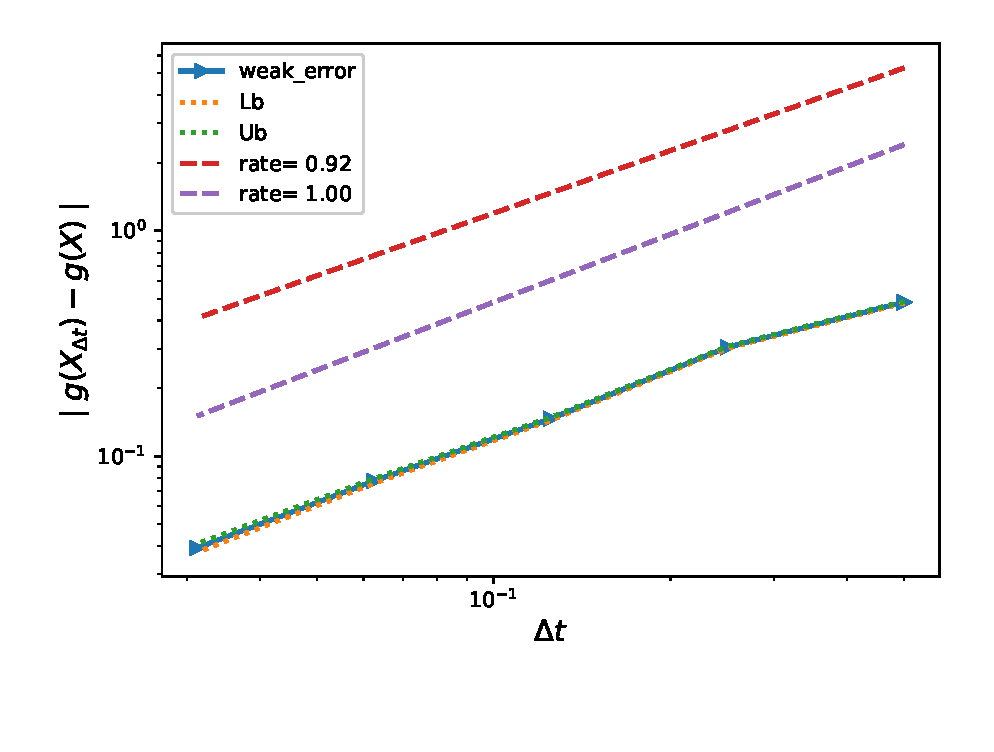
\includegraphics[width=1\linewidth]{./figures/rBergomi_weak_error_rates/without_richardson/H_043/weak_convergence_order_Bergomi_H_043_K_1_M_10_6_CI_relative}
		\caption{}
		\label{fig:sub3}
	\end{subfigure}%
	\begin{subfigure}{.4\textwidth}
		\centering
		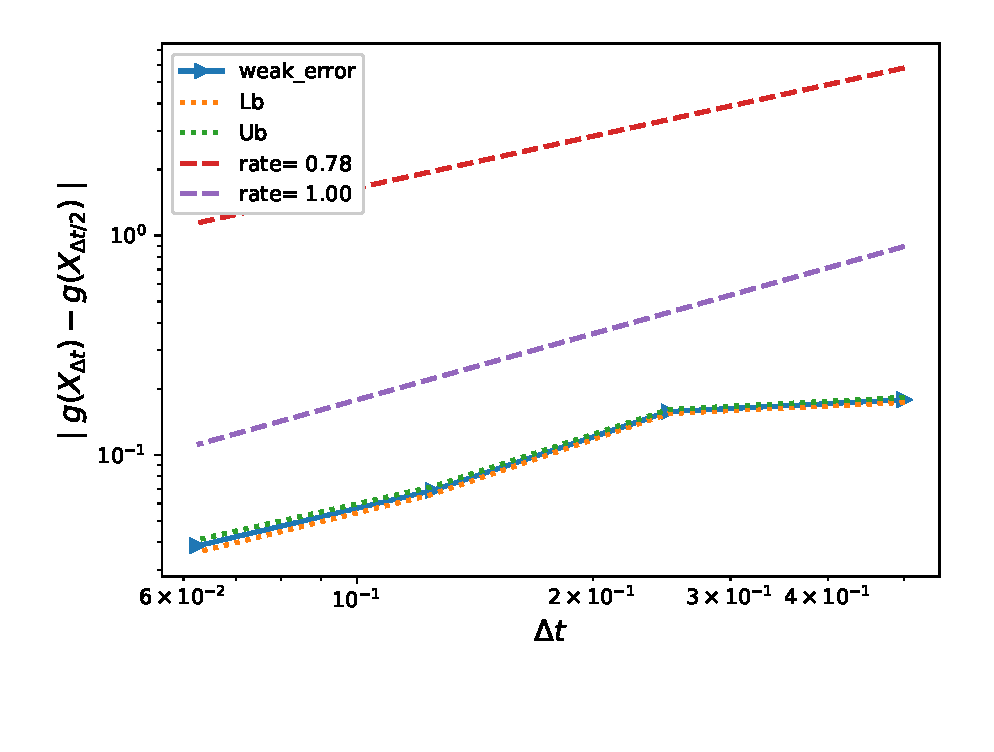
\includegraphics[width=1\linewidth]{./figures/rBergomi_weak_error_rates/without_richardson/H_043/weak_convergence_order_differences_Bergomi_H_043_K_1_M_10_6_CI_relative}
		\caption{}
		\label{fig:sub4}
	\end{subfigure}
	
	\caption{The rate of convergence of the weak error for set $1$ parameters in table \ref{table:Reference solution, using MC with $500$ time steps, of Call option price under rBergomi model, for different parameter constellation.}, without Richardson extraploation, using MC with $M=10^6$: a) $\abs{\expt{g(X_{\Delta t})}-g(X)}$  b) $\abs{\expt{g(X_{\Delta t})-g(X_{\Delta t/2})}}$ }
	\label{fig:Weak_rate_H_043_without_rich}
\end{figure}

\begin{figure}[h!]
	\centering
	\begin{subfigure}{.4\textwidth}
		\centering
		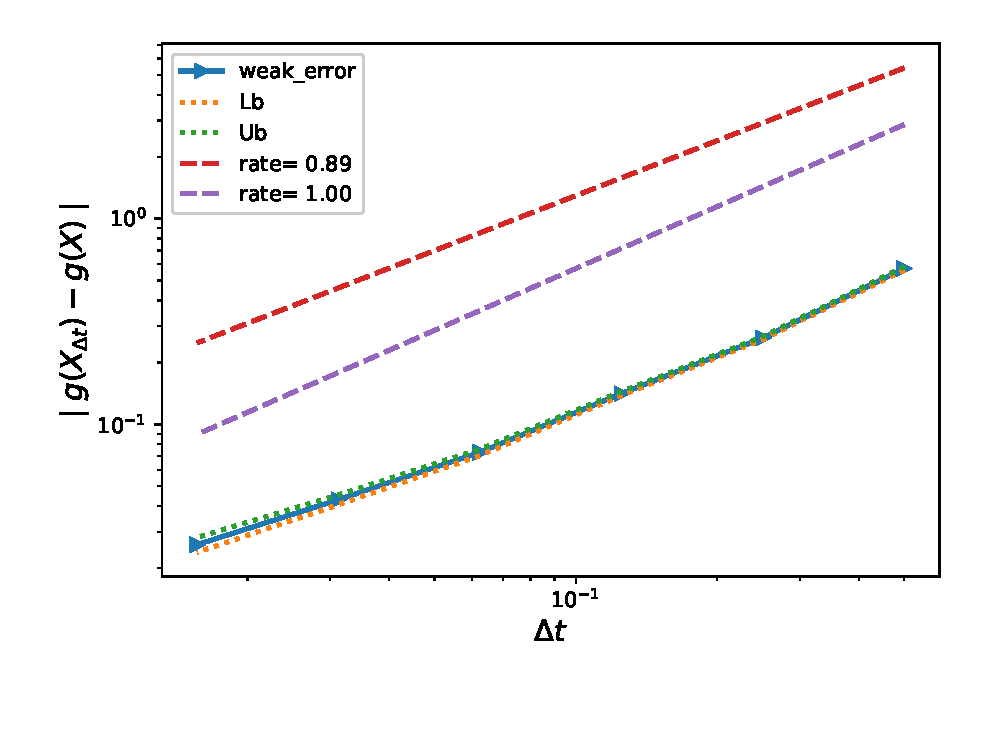
\includegraphics[width=1\linewidth]{./figures/rBergomi_weak_error_rates/without_richardson/H_007/weak_convergence_order_Bergomi_H_007_K_1_M_10_6_CI_relative}
		\caption{}
		\label{fig:sub3}
	\end{subfigure}%
	\begin{subfigure}{.4\textwidth}
		\centering
		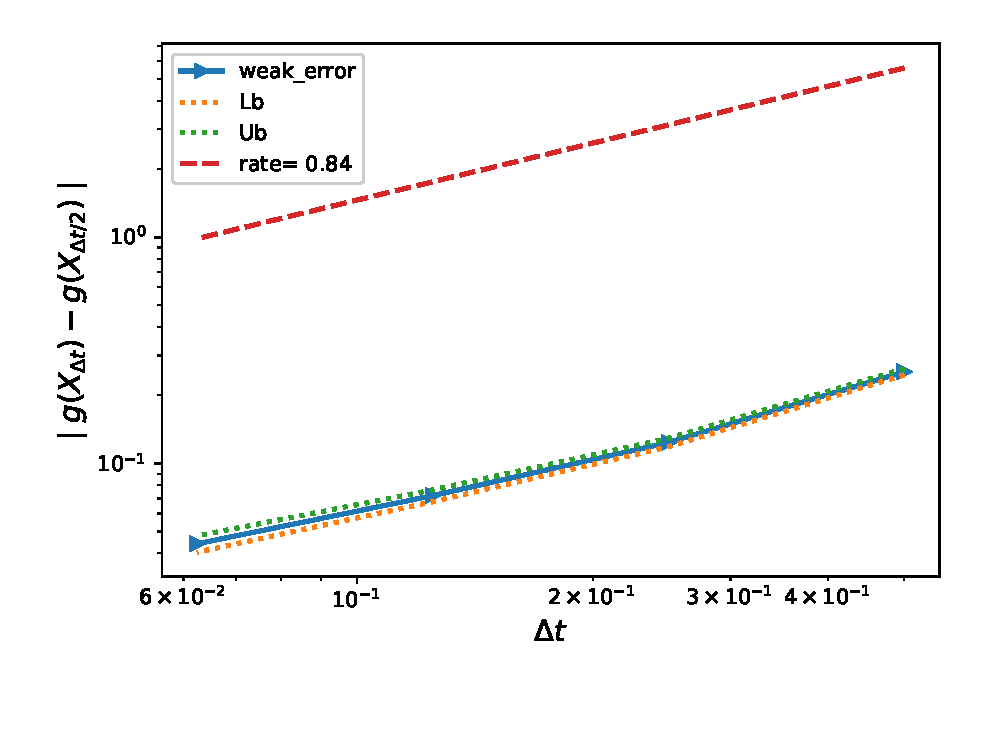
\includegraphics[width=1\linewidth]{./figures/rBergomi_weak_error_rates/without_richardson/H_007/weak_convergence_order_differences_Bergomi_H_007_K_1_M_10_6_CI_relative}
		\caption{}
		\label{fig:sub4}
	\end{subfigure}
	
	\caption{The rate of convergence of the weak error for set $2$ parameters in table \ref{table:Reference solution, using MC with $500$ time steps, of Call option price under rBergomi model, for different parameter constellation.}, without Richardson extraploation, using MC with $M=10^6$: a) $\abs{\expt{g(X_{\Delta t})}-g(X)}$  b) $\abs{\expt{g(X_{\Delta t})-g(X_{\Delta t/2})}}$ }
	\label{fig:Weak_rate_H_007_without_rich}
\end{figure}



%\begin{figure}[!h]
%	\centering
%	\begin{subfigure}{.4\textwidth}
%		\centering
%		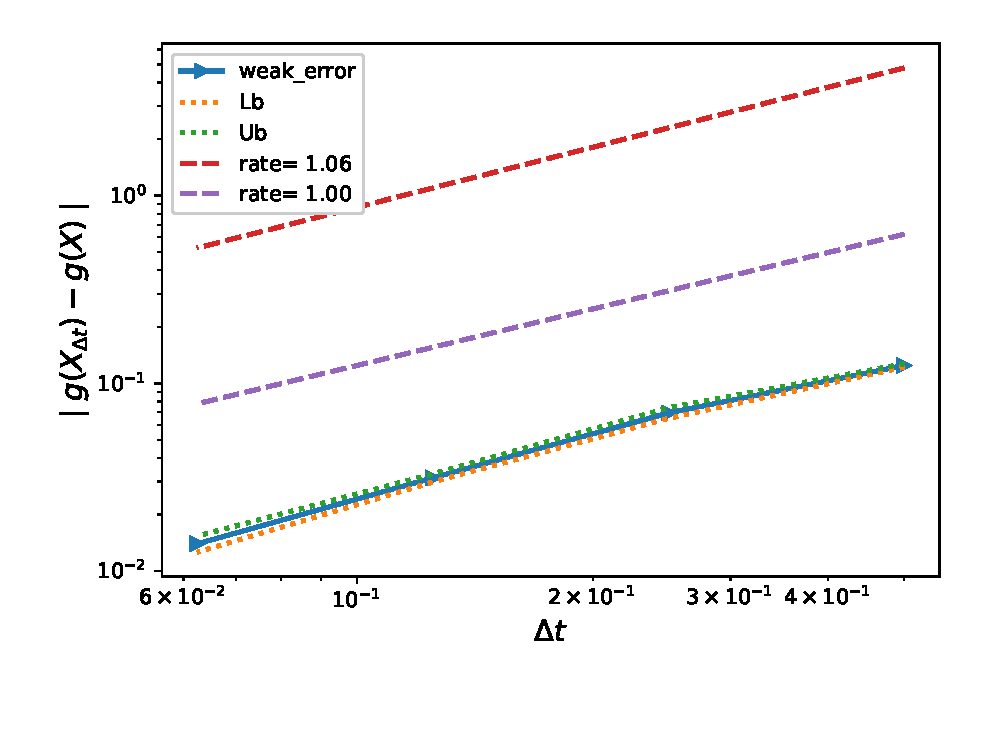
\includegraphics[width=1\linewidth]{./figures/rBergomi_weak_error_rates/without_richardson/H_007/weak_convergence_order_Bergomi_H_007_K_08_M_10_6_CI_relative}
%		\caption{}
%		\label{fig:sub3}
%	\end{subfigure}%
%	\begin{subfigure}{.4\textwidth}
%		\centering
%		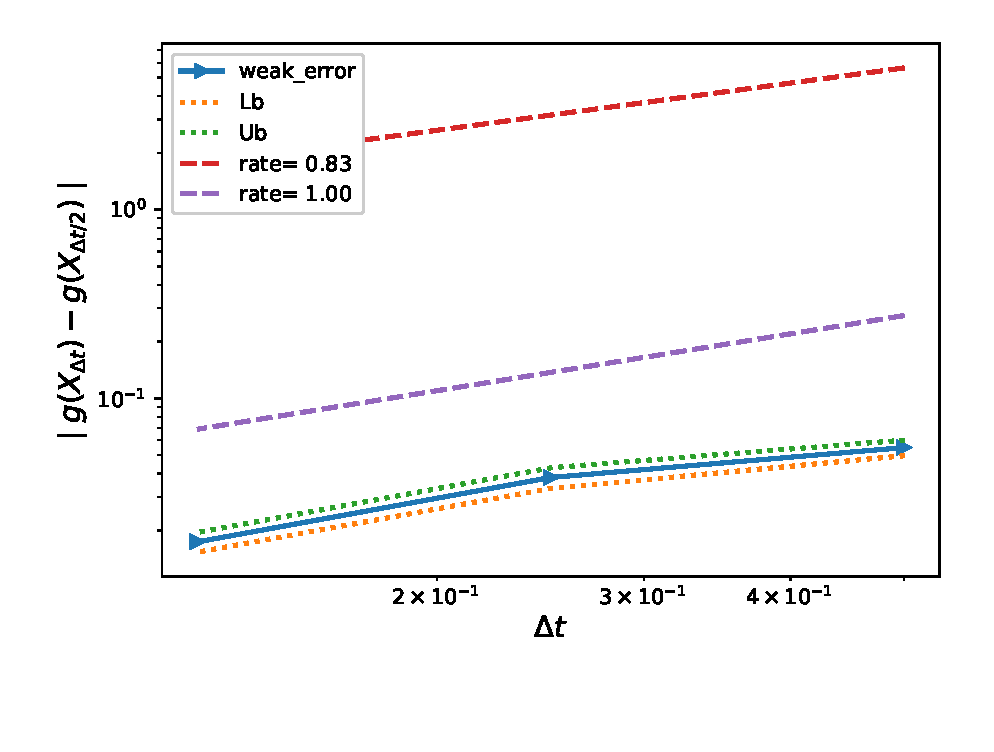
\includegraphics[width=1\linewidth]{./figures/rBergomi_weak_error_rates/without_richardson/H_007/weak_convergence_order_differences_Bergomi_H_007_K_08_M_10_6_CI_relative}
%		\caption{}
%		\label{fig:sub4}
%	\end{subfigure}
%	
%	\caption{The rate of convergence of the weak error for set $3$ parameters in table \ref{table:Reference solution, using MC with $500$ time steps, of Call option price under rBergomi model, for different parameter constellation.}, without Richardson extraploation, using MC with $M=10^6$: a) $\abs{\expt{g(X_{\Delta t})}-g(X)}$  b) $\abs{\expt{g(X_{\Delta t})-g(X_{\Delta t/2})}}$ }
%	\label{fig:Weak_rate_H_007_without_rich_K_08}
%\end{figure}
%
%
%
%
%
%
%\begin{figure}[!htbp]
%	\centering
%	\begin{subfigure}{.4\textwidth}
%		\centering
%		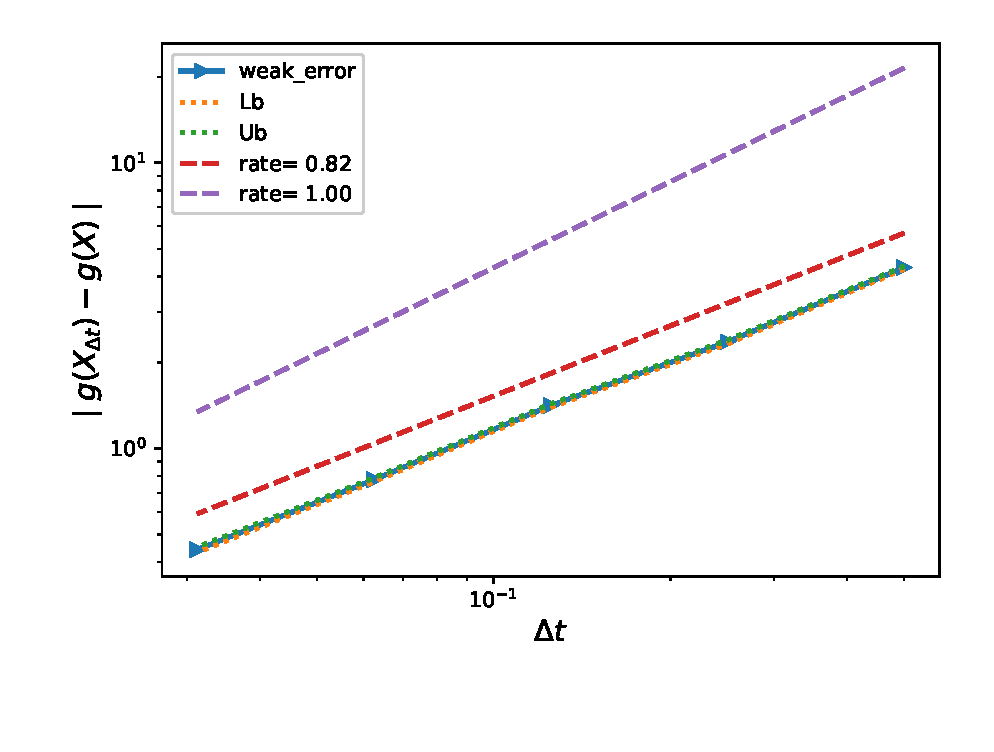
\includegraphics[width=1\linewidth]{./figures/rBergomi_weak_error_rates/without_richardson/H_007/weak_convergence_order_Bergomi_H_007_K_12_M_10_6_CI_relative}
%		\caption{}
%		\label{fig:sub3}
%	\end{subfigure}%
%	\begin{subfigure}{.4\textwidth}
%		\centering
%		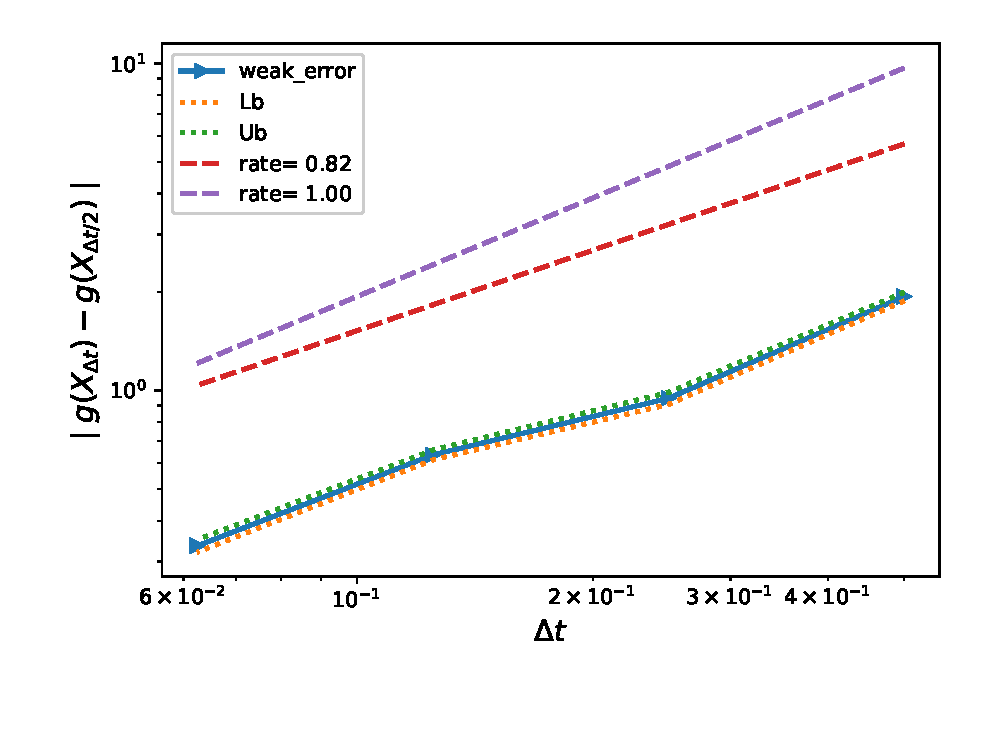
\includegraphics[width=1\linewidth]{./figures/rBergomi_weak_error_rates/without_richardson/H_007/weak_convergence_order_differences_Bergomi_H_007_K_12_M_10_6_CI_relative}
%		\caption{}
%		\label{fig:sub4}
%	\end{subfigure}
%	
%	\caption{The rate of convergence of the weak error for set $4$ parameters in table \ref{table:Reference solution, using MC with $500$ time steps, of Call option price under rBergomi model, for different parameter constellation.}, without Richardson extraploation, using MC with $M=10^6$: a) $\abs{\expt{g(X_{\Delta t})}-g(X)}$  b) $\abs{\expt{g(X_{\Delta t})-g(X_{\Delta t/2})}}$ }
%	\label{fig:Weak_rate_H_007_without_rich_K_12}
%\end{figure}
%

\begin{figure}[!htb]
	\centering
	\begin{subfigure}{.4\textwidth}
		\centering
		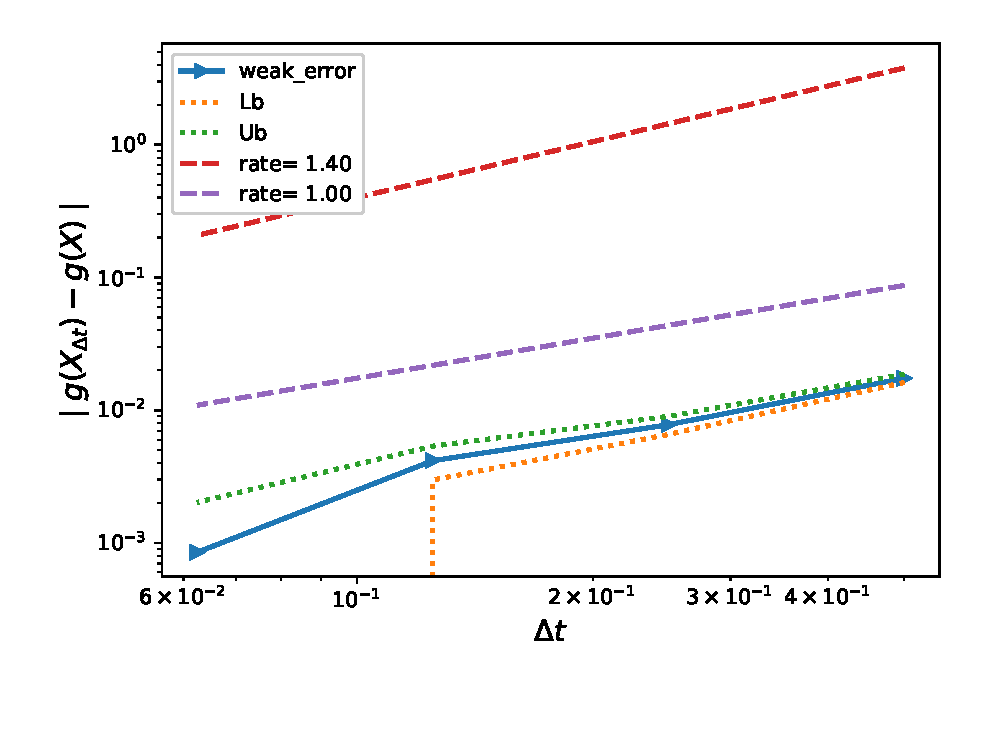
\includegraphics[width=1\linewidth]{./figures/rBergomi_weak_error_rates/without_richardson/H_002/weak_convergence_order_Bergomi_H_002_K_1_M_3_10_6_CI_relative}
		\caption{}
		\label{fig:sub3}
	\end{subfigure}%
	\begin{subfigure}{.4\textwidth}
		\centering
		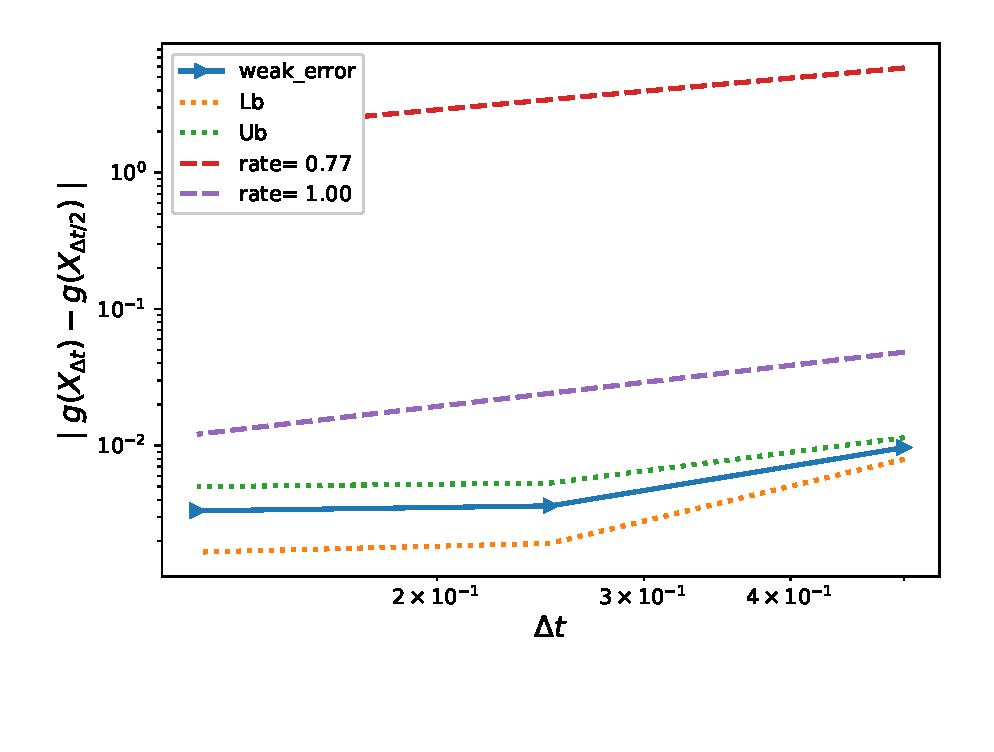
\includegraphics[width=1\linewidth]{./figures/rBergomi_weak_error_rates/without_richardson/H_002/weak_convergence_order_differences_Bergomi_H_002_K_1_M_3_10_6_CI_relative}
		\caption{}
		\label{fig:sub4}
	\end{subfigure}
	
	\caption{The rate of convergence of the weak error for set $5$ parameters in table \ref{table:Reference solution, using MC with $500$ time steps, of Call option price under rBergomi model, for different parameter constellation.}, without Richardson extraploation, using MC with $M=3.10^6$: a) $\abs{\expt{g(X_{\Delta t})}-g(X)}$  b) $\abs{\expt{g(X_{\Delta t})-g(X_{\Delta t/2})}}$ }
	\label{fig:Weak_rate_H_002_without_rich_K_1}
\end{figure}






\begin{figure}[!htb]
	\centering
	\begin{subfigure}{.4\textwidth}
		\centering
		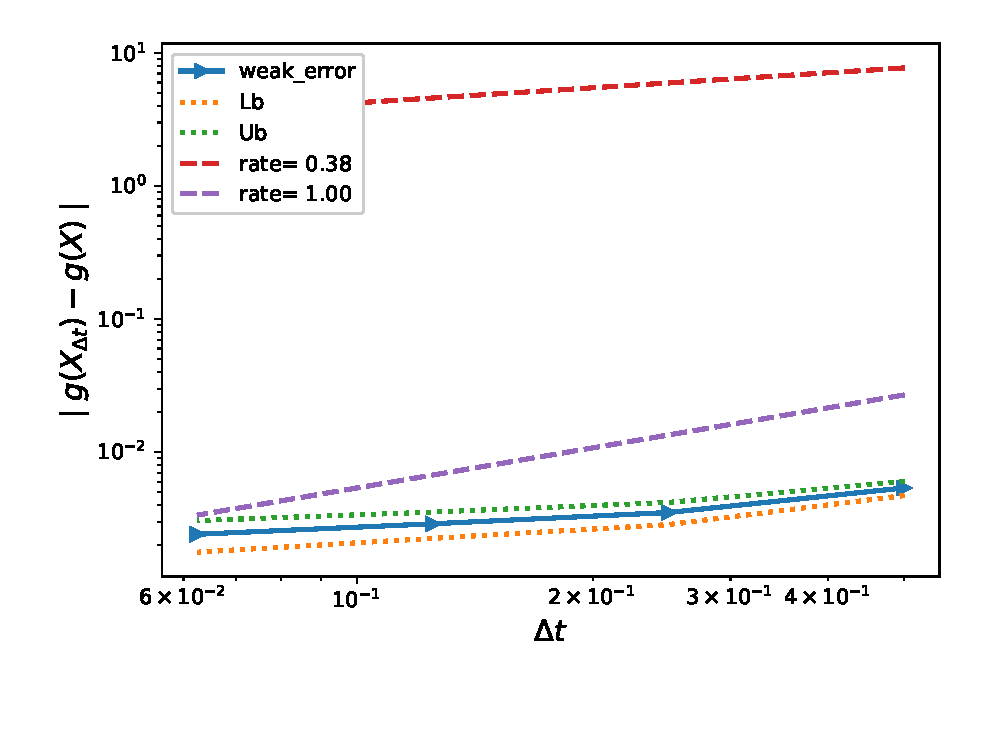
\includegraphics[width=1\linewidth]{./figures/rBergomi_weak_error_rates/without_richardson/H_002/weak_convergence_order_Bergomi_H_002_K_08_M_5_10_6_CI_relative}
		\caption{}
		\label{fig:sub3}
	\end{subfigure}%
	\begin{subfigure}{.4\textwidth}
		\centering
		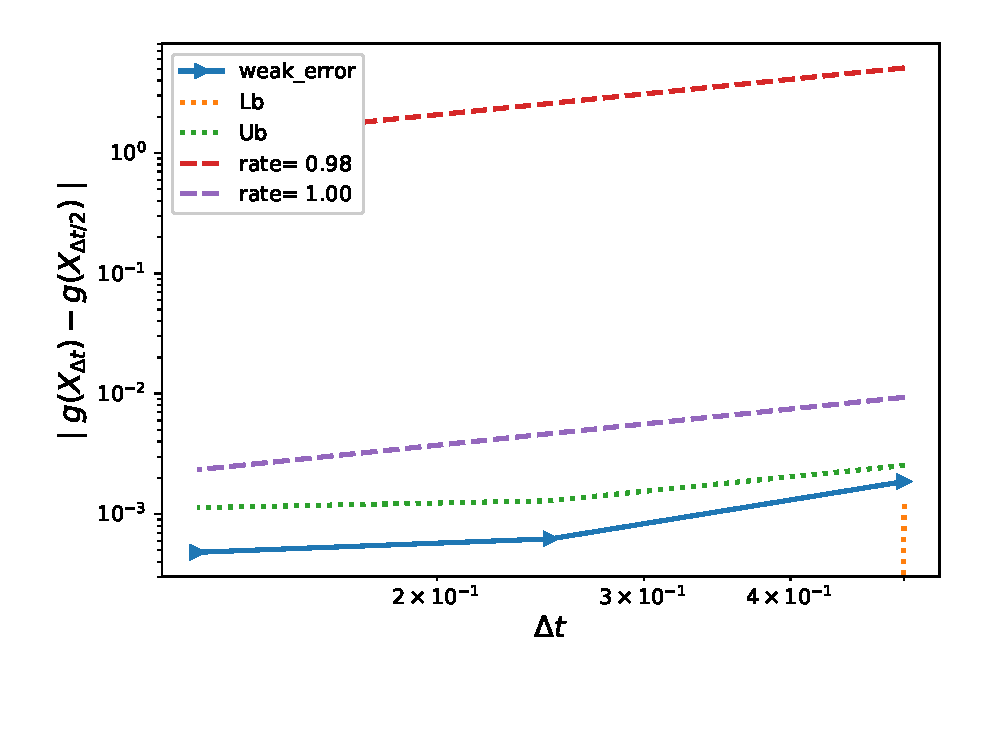
\includegraphics[width=1\linewidth]{./figures/rBergomi_weak_error_rates/without_richardson/H_002/weak_convergence_order_differences_Bergomi_H_002_K_08_M_5_10_6_CI_relative}
		\caption{}
		\label{fig:sub4}
	\end{subfigure}
	
	\caption{The rate of convergence of the weak error for set $6$ parameters in table \ref{table:Reference solution, using MC with $500$ time steps, of Call option price under rBergomi model, for different parameter constellation.}, without Richardson extraploation, using MC with $M=5.10^6$: a) $\abs{\expt{g(X_{\Delta t})}-g(X)}$  b) $\abs{\expt{g(X_{\Delta t})-g(X_{\Delta t/2})}}$ }
	\label{fig:Weak_rate_H_002_without_rich_K_08}
\end{figure}




\begin{figure}[!htb]
	\centering
	\begin{subfigure}{.4\textwidth}
		\centering
		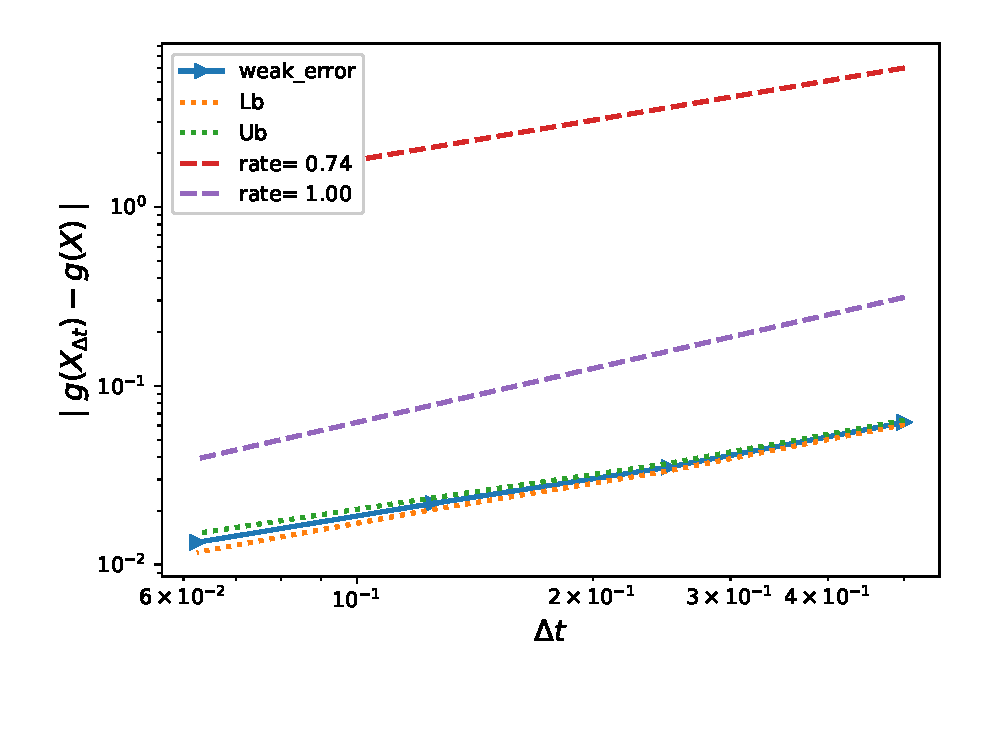
\includegraphics[width=1\linewidth]{./figures/rBergomi_weak_error_rates/without_richardson/H_002/weak_convergence_order_Bergomi_H_002_K_12_M_3_10_6_CI_relative}
		\caption{}
		\label{fig:sub3}
	\end{subfigure}%
	\begin{subfigure}{.4\textwidth}
		\centering
		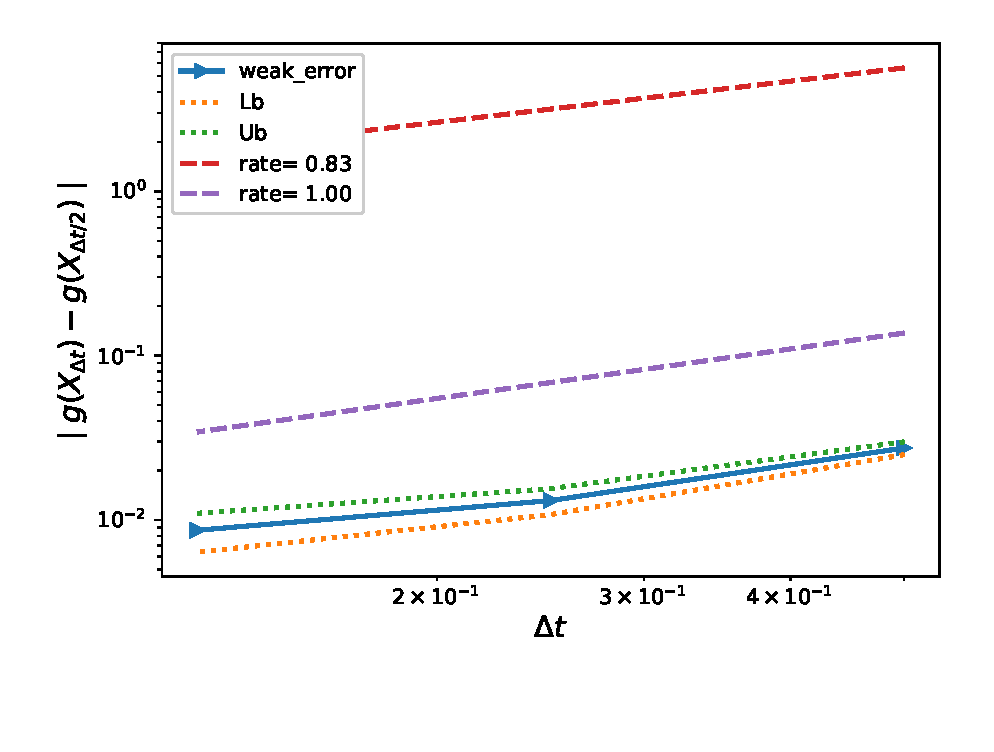
\includegraphics[width=1\linewidth]{./figures/rBergomi_weak_error_rates/without_richardson/H_002/weak_convergence_order_differences_Bergomi_H_002_K_12_M_3_10_6_CI_relative}
		\caption{}
		\label{fig:sub4}
	\end{subfigure}
	
	\caption{The rate of convergence of the weak error for set $7$ parameters in table \ref{table:Reference solution, using MC with $500$ time steps, of Call option price under rBergomi model, for different parameter constellation.}, without Richardson extraploation, using MC with $M=5.10^6$: a) $\abs{\expt{g(X_{\Delta t})}-g(X)}$  b) $\abs{\expt{g(X_{\Delta t})-g(X_{\Delta t/2})}}$ }
	\label{fig:Weak_rate_H_002_without_rich_K_12}
\end{figure}


\FloatBarrier


\subsubsection{With Richardson extrapolation (level 1)}
From figures (\ref{fig:Weak_rate_H_043_with_rich}, \ref{fig:Weak_rate_H_007_with_rich}, \ref{fig:Weak_rate_H_002_with_rich_K1}), we see that for all cases, we get a weak error of order around $\Delta t^2$. The upper and lower bounds are $95\%$ confidence interval.
\begin{figure}[h!]
	\centering
	\begin{subfigure}{.4\textwidth}
		\centering
		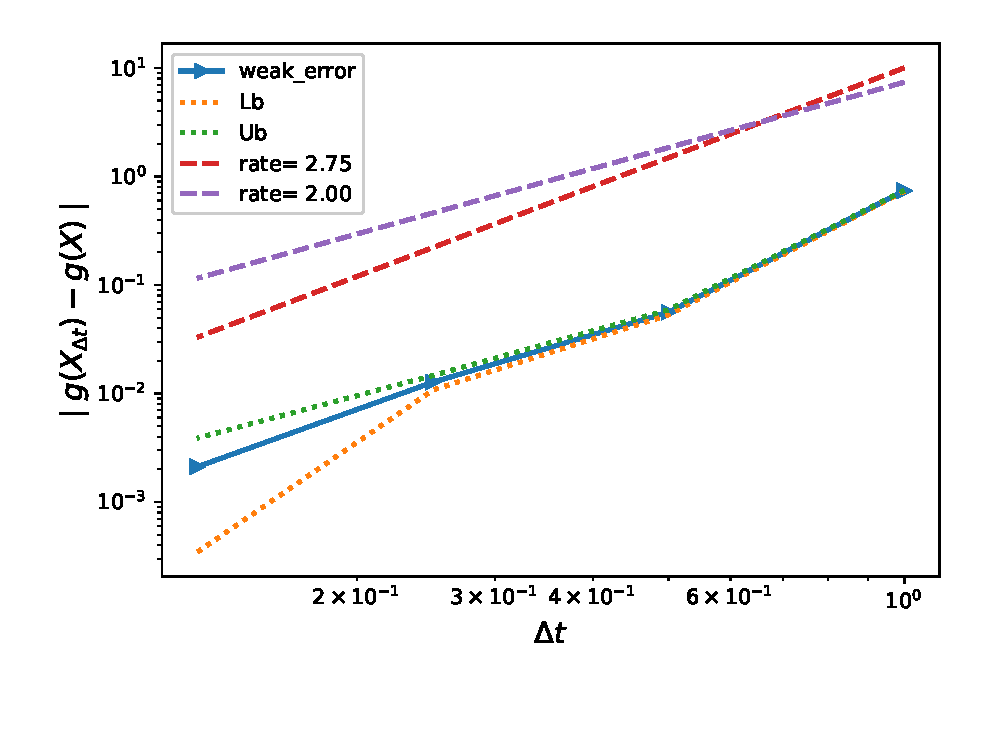
\includegraphics[width=1\linewidth]{./figures/rBergomi_weak_error_rates/with_richardson/H_043/weak_convergence_order_Bergomi_H_043_K_1_M_10_6_richardson_relative}
		\caption{}
		\label{fig:sub3}
	\end{subfigure}%
	\begin{subfigure}{.4\textwidth}
		\centering
		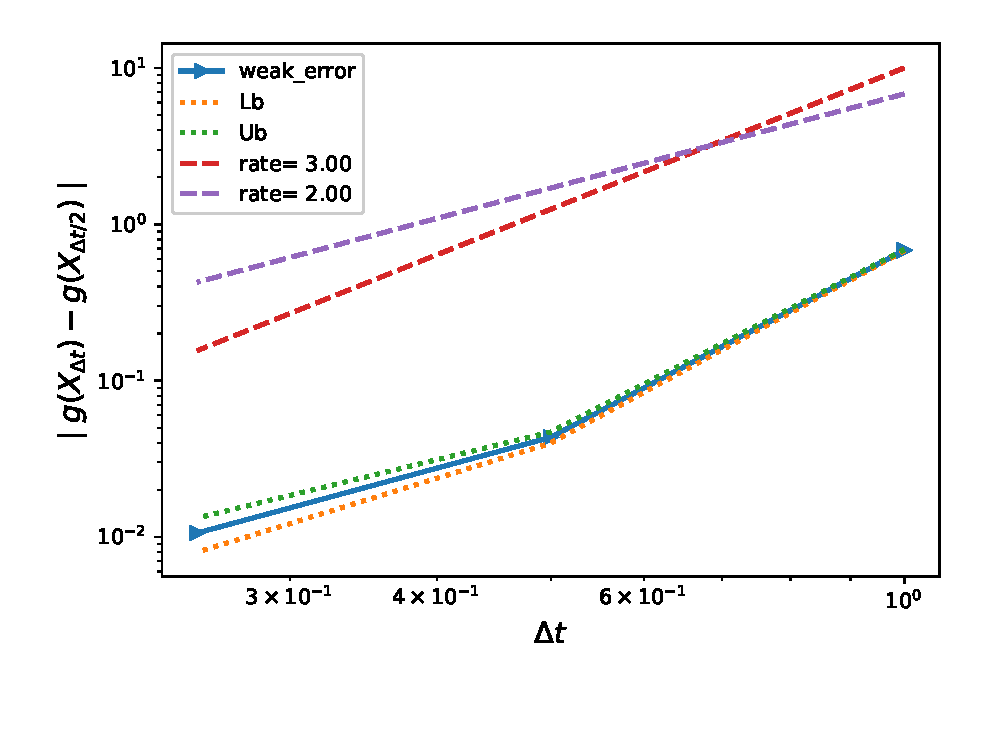
\includegraphics[width=1\linewidth]{./figures/rBergomi_weak_error_rates/with_richardson/H_043/weak_convergence_order_differences_Bergomi_H_043_K_1_M_10_6_richardson_relative}
		\caption{}
		\label{fig:sub4}
	\end{subfigure}
	
	\caption{The rate of convergence of the weak error for set $1$ parameters in table \ref{table:Reference solution, using MC with $500$ time steps, of Call option price under rBergomi model, for different parameter constellation.}, with Richardson extraploation, using MC with $M=10^6$: a) $\abs{\expt{2 g(X_{\Delta t/2}) -g(X_{\Delta t})}-g(X)}$  b) $\abs{\expt{3 g(X_{\Delta t/2})-g(X_{\Delta t})-2 g(X_{\Delta t/4})}}$ }
	\label{fig:Weak_rate_H_043_with_rich}
\end{figure}

\begin{figure}[h!]
	\centering
	\begin{subfigure}{.4\textwidth}
		\centering
		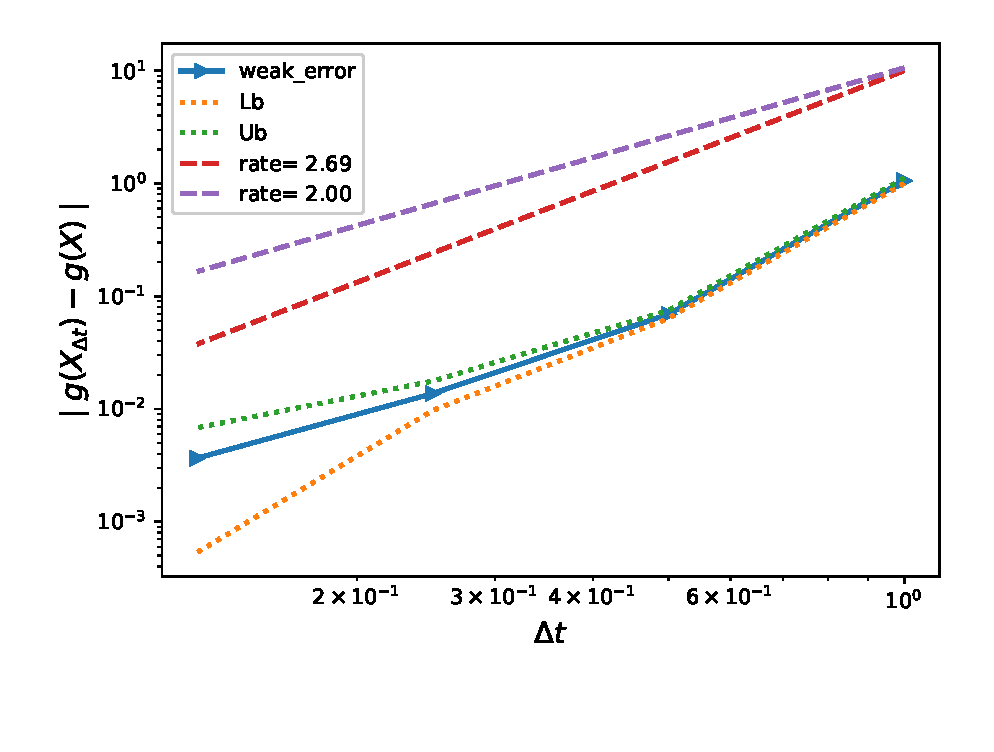
\includegraphics[width=1\linewidth]{./figures/rBergomi_weak_error_rates/with_richardson/H_007/weak_convergence_order_Bergomi_H_007_K_1_richardson_relative_M_10_6}
		\caption{}
		\label{fig:sub3}
	\end{subfigure}%
	\begin{subfigure}{.4\textwidth}
		\centering
		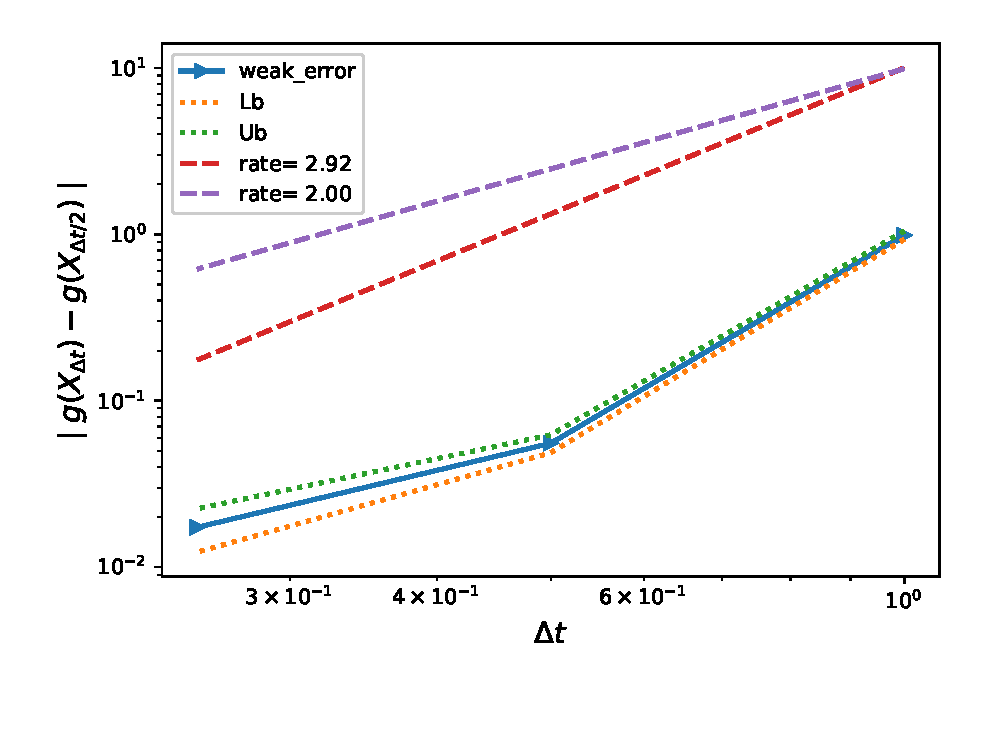
\includegraphics[width=1\linewidth]{./figures/rBergomi_weak_error_rates/with_richardson/H_007/weak_convergence_order_differences_Bergomi_H_007_K_1_richardson_relative_M_10_6}
		\caption{}
		\label{fig:sub4}
	\end{subfigure}
	
	\caption{The rate of convergence of the weak error for set $2$ parameters in table \ref{table:Reference solution, using MC with $500$ time steps, of Call option price under rBergomi model, for different parameter constellation.}, with Richardson extraploation, using MC with $M=10^6$: a) $\abs{\expt{2 g(X_{\Delta t/2}) -g(X_{\Delta t})}-g(X)}$  b) $\abs{\expt{3 g(X_{\Delta t/2})-g(X_{\Delta t})-2 g(X_{\Delta t/4})}}$ }
	\label{fig:Weak_rate_H_007_with_rich}
\end{figure}

%\begin{figure}[!htbp]
%	\centering
%	\begin{subfigure}{.4\textwidth}
%		\centering
%		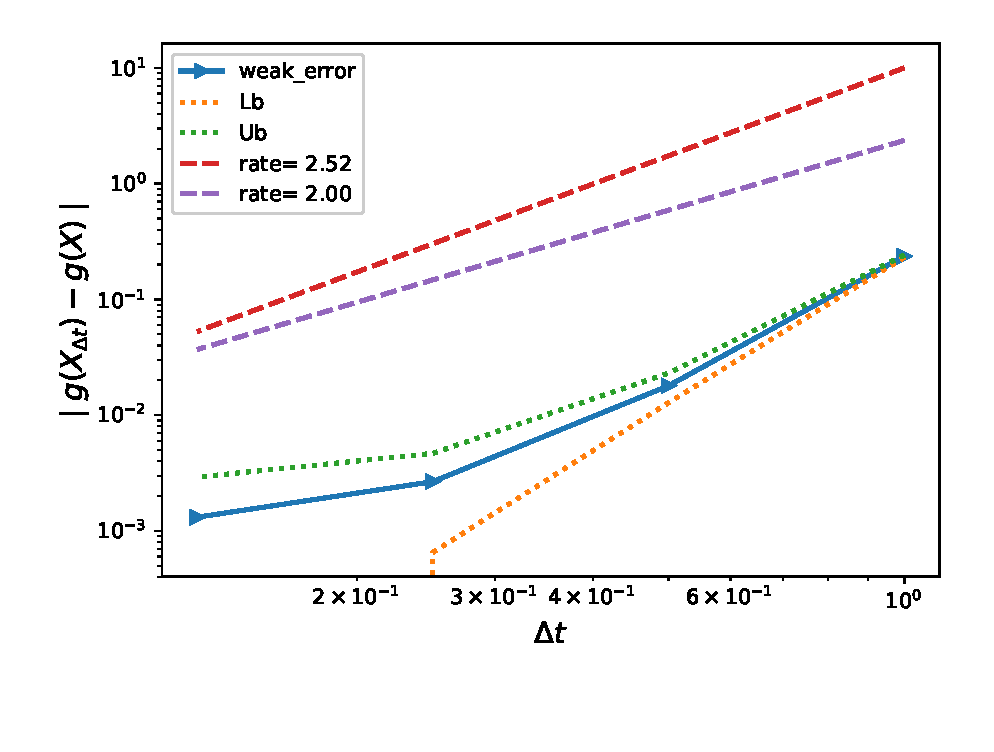
\includegraphics[width=1\linewidth]{./figures/rBergomi_weak_error_rates/with_richardson/H_007/weak_convergence_order_Bergomi_H_007_K_08_M_10_6_richardson_relative}
%		\caption{}
%		\label{fig:sub3}
%	\end{subfigure}%
%	\begin{subfigure}{.4\textwidth}
%		\centering
%		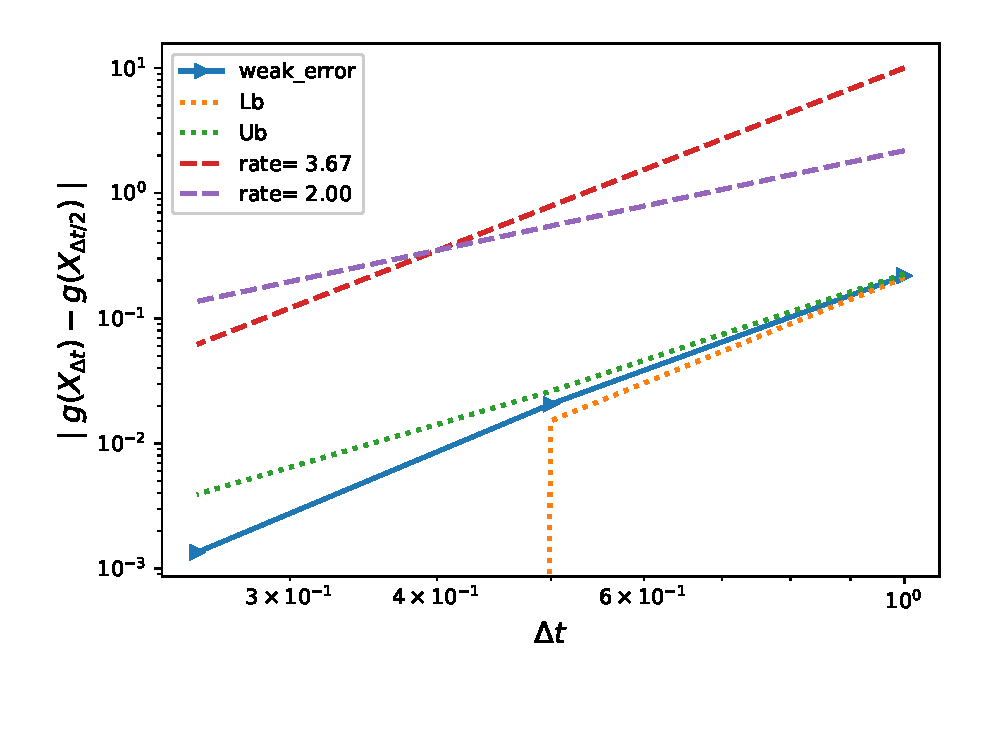
\includegraphics[width=1\linewidth]{./figures/rBergomi_weak_error_rates/with_richardson/H_007/weak_convergence_order_differences_Bergomi_H_007_K_08_M_10_6_richardson_relative}
%		\caption{}
%		\label{fig:sub4}
%	\end{subfigure}
%	
%
%	\caption{The rate of convergence of the weak error for set $3$ parameters in table \ref{table:Reference solution, using MC with $500$ time steps, of Call option price under rBergomi model, for different parameter constellation.}, with Richardson extraploation, using MC with $M=10^6$: a) $\abs{\expt{2 g(X_{\Delta t/2}) -g(X_{\Delta t})}-g(X)}$  b) $\abs{\expt{3 g(X_{\Delta t/2})-g(X_{\Delta t})-2 g(X_{\Delta t/4})}}$ }
%	\label{fig:Weak_rate_H_007_with_rich_K08}
%\end{figure}
%
%
%
%
%\begin{figure}[!htbp]
%	\centering
%	\begin{subfigure}{.4\textwidth}
%		\centering
%		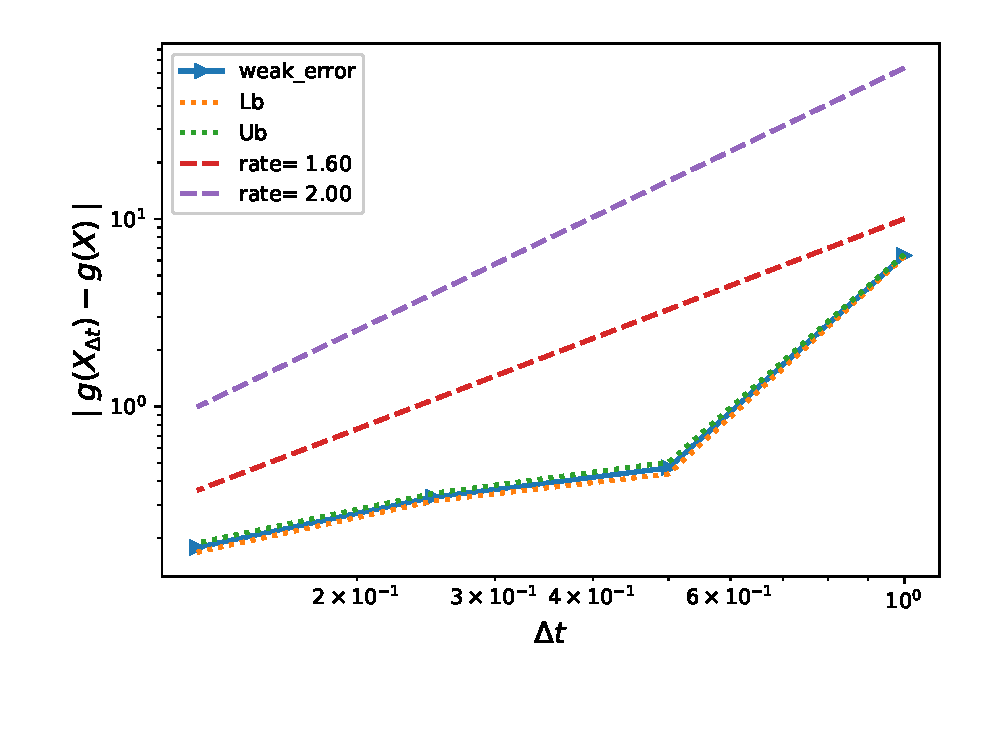
\includegraphics[width=1\linewidth]{./figures/rBergomi_weak_error_rates/with_richardson/H_007/weak_convergence_order_Bergomi_H_007_K_12_M_2_10_6_richardson_relative}
%		\caption{}
%		\label{fig:sub3}
%	\end{subfigure}%
%	\begin{subfigure}{.4\textwidth}
%		\centering
%		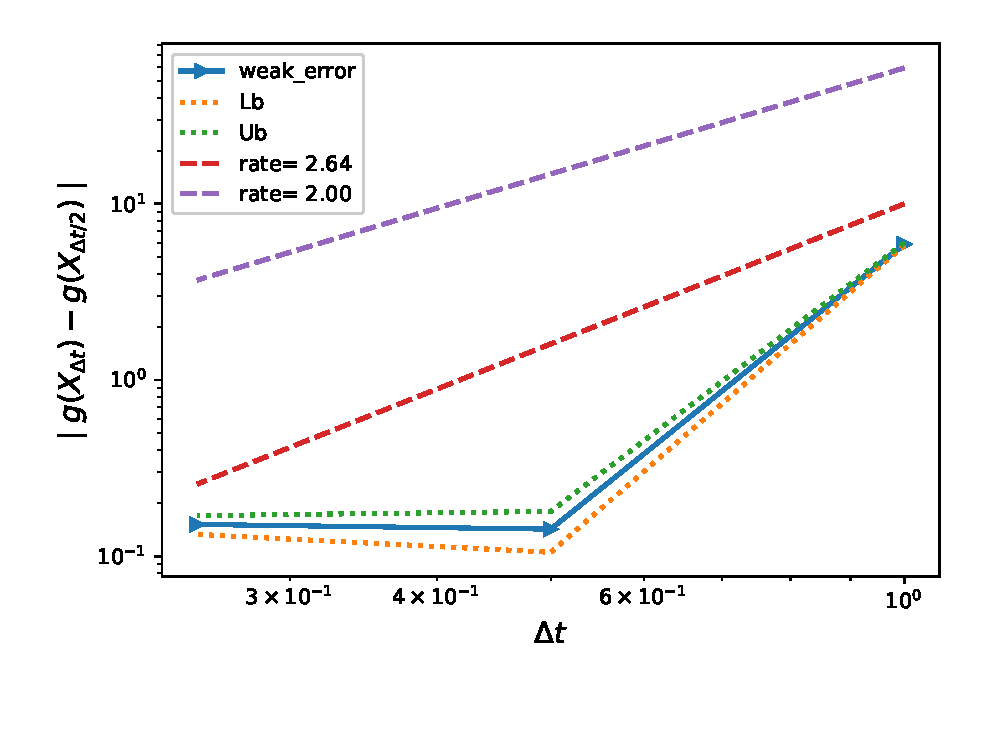
\includegraphics[width=1\linewidth]{./figures/rBergomi_weak_error_rates/with_richardson/H_007/weak_convergence_order_differences_Bergomi_H_007_K_12_M_2_10_6_richardson_relative}
%		\caption{}
%		\label{fig:sub4}
%	\end{subfigure}
%	
%	\caption{The rate of convergence of the weak error for set $4$ parameters in table \ref{table:Reference solution, using MC with $500$ time steps, of Call option price under rBergomi model, for different parameter constellation.}, with Richardson extraploation, using MC with $M=2.10^6$: a) $\abs{\expt{2 g(X_{\Delta t/2}) -g(X_{\Delta t})}-g(X)}$  b) $\abs{\expt{3 g(X_{\Delta t/2})-g(X_{\Delta t})-2 g(X_{\Delta t/4})}}$ }
%	\label{fig:Weak_rate_H_007_with_rich_K12}
%\end{figure}
%
%
%



\begin{figure}[!htbp]
	\centering
	\begin{subfigure}{.4\textwidth}
		\centering
		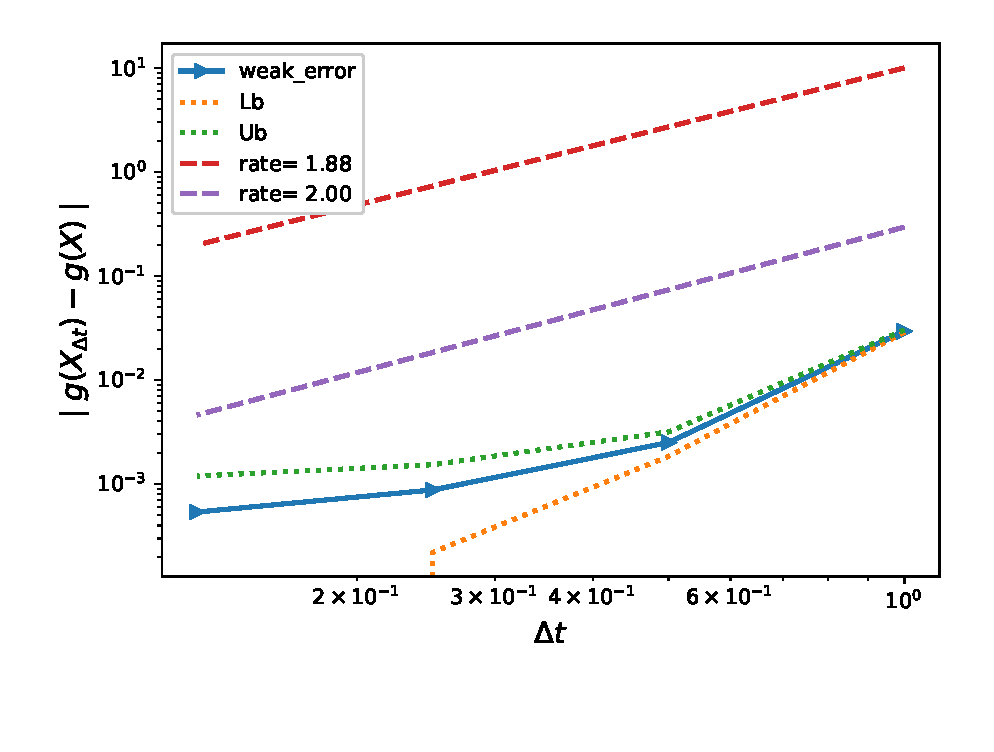
\includegraphics[width=1\linewidth]{./figures/rBergomi_weak_error_rates/with_richardson/H_002/weak_convergence_order_Bergomi_H_002_K_1_M_1_10_7_richardson_relative}
		\caption{}
		\label{fig:sub3}
	\end{subfigure}%
	\begin{subfigure}{.4\textwidth}
		\centering
		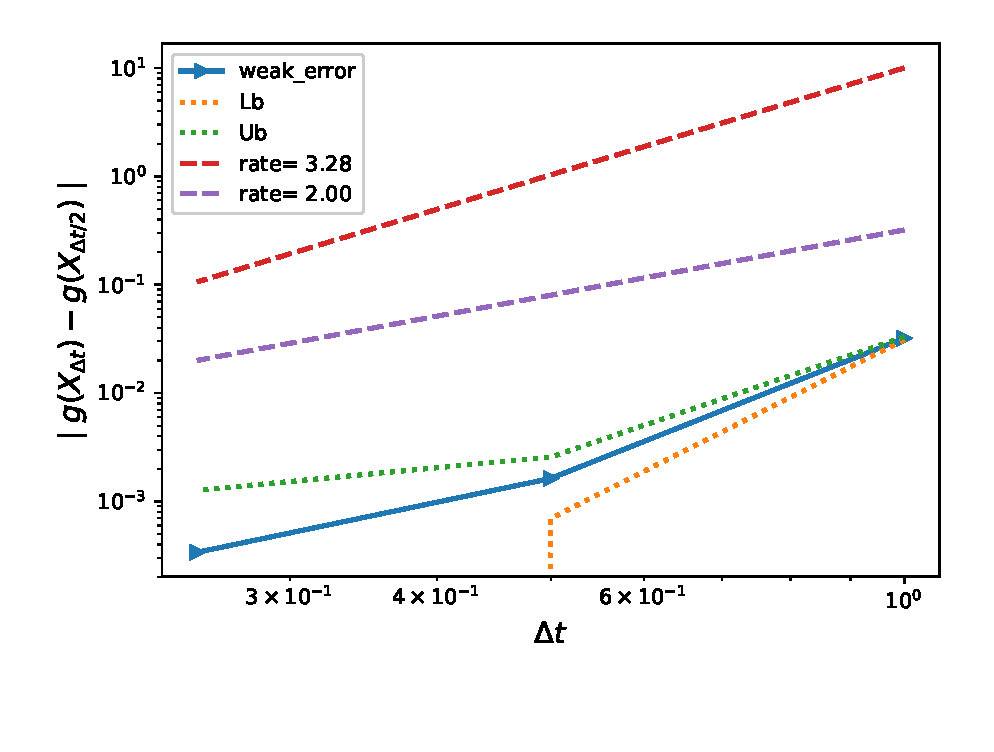
\includegraphics[width=1\linewidth]{./figures/rBergomi_weak_error_rates/with_richardson/H_002/weak_convergence_order_differences_Bergomi_H_002_K_1_M_1_10_7_richardson_relative}
		\caption{}
		\label{fig:sub4}
	\end{subfigure}
	
	\caption{The rate of convergence of the weak error for set $5$ parameters in table \ref{table:Reference solution, using MC with $500$ time steps, of Call option price under rBergomi model, for different parameter constellation.}, with Richardson extraploation, using MC with $M=10^7$: a) $\abs{\expt{2 g(X_{\Delta t/2}) -g(X_{\Delta t})}-g(X)}$  b) $\abs{\expt{3 g(X_{\Delta t/2})-g(X_{\Delta t})-2 g(X_{\Delta t/4})}}$ }
	\label{fig:Weak_rate_H_002_with_rich_K1}
\end{figure}
\FloatBarrier


%\newpage
%\subsubsection*{With Richardson extrapolation (level 2)}
%From figures (\ref{fig:Weak_rate_H_043_with_rich_level2} and \ref{fig:Weak_rate_H_007_with_rich_level2}), we see that for both cases $H \in \{0.43,0.07\}$, we get a non precise estimate of weak error, even with $M=10^6$ samples, due to the high statistical error. The upper and lower bounds are $95\%$ confidence interval. For later reported values in Section \ref{sec:Comparing relative errors}, we extrapolate the first estimated value, with $1$ time step at the coarse level, assuming a rate of weak error of order $\Delta t ^3$.
%
%\begin{figure}[h!]
%	\centering
%	\begin{subfigure}{.4\textwidth}
%		\centering
%		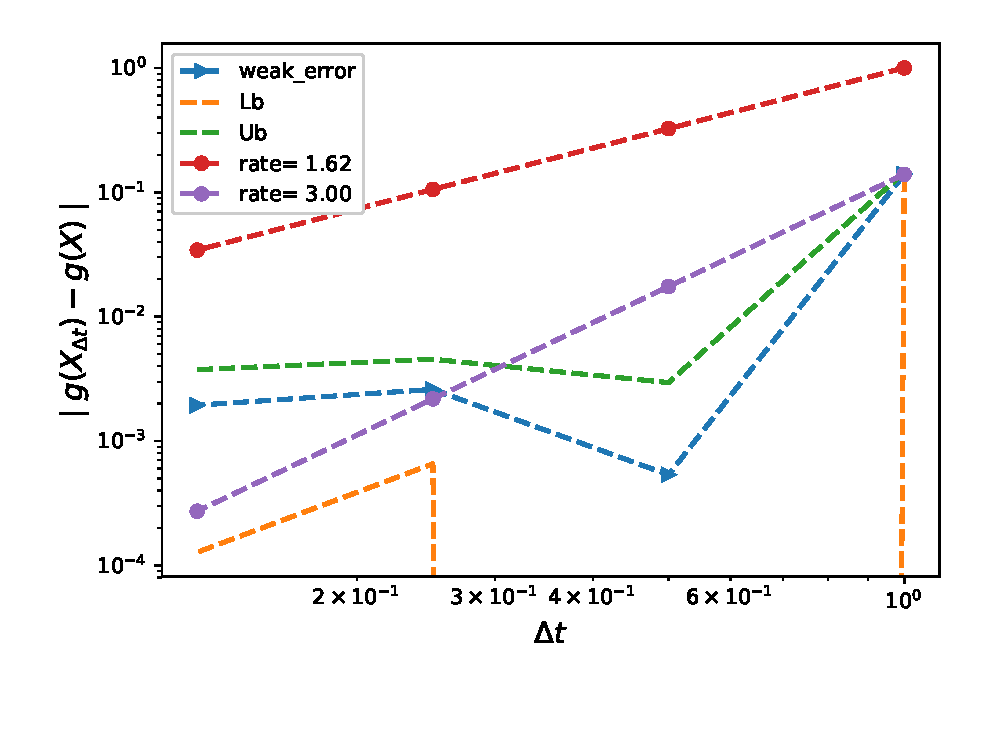
\includegraphics[width=1\linewidth]{./figures/rBergomi_weak_error_rates/with_richardson/H_043/weak_convergence_order_Bergomi_H_043_K_1_richardson_level2_relative_M_10_6}
%		\caption{}
%		\label{fig:sub3}
%	\end{subfigure}%
%	\begin{subfigure}{.4\textwidth}
%		\centering
%		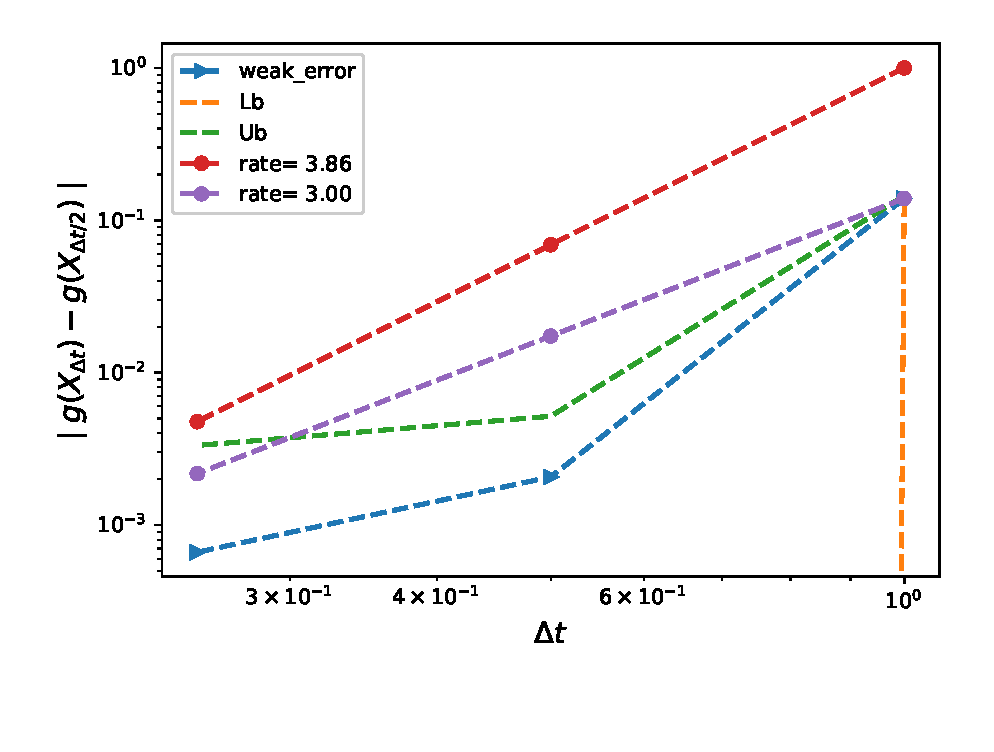
\includegraphics[width=1\linewidth]{./figures/rBergomi_weak_error_rates/with_richardson/H_043/weak_convergence_order_differences_Bergomi_H_043_K_1_richardson_level2_relative_M_10_6}
%		\caption{}
%		\label{fig:sub4}
%	\end{subfigure}
%	
%	\caption{The rate of convergence of the weak error for $H=0.43$ $K=1$, with Richardson extraploation, using MC with $M=10^6$: a) $\abs{\frac{1}{3}\expt{8 g(X_{\Delta t/4}) -6g(X_{\Delta t/2}) +g(X_{\Delta t})}-g(X)}$  b) $\abs{\frac{1}{3}\expt{-8 g(X_{\Delta t/8}) +14g(X_{\Delta t/4})-7 (X_{\Delta t/2}) +g(X_{\Delta t})}}$}
%	\label{fig:Weak_rate_H_043_with_rich_level2}
%\end{figure}
%
%\begin{figure}[h!]
%	\centering
%	\begin{subfigure}{.4\textwidth}
%		\centering
%		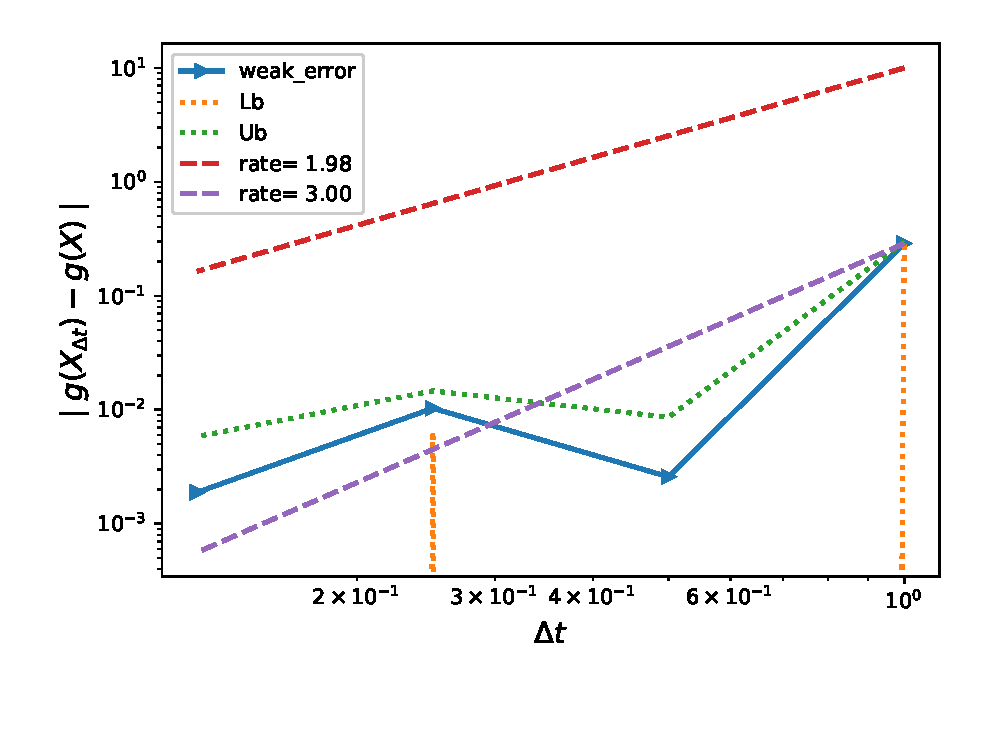
\includegraphics[width=1\linewidth]{./figures/rBergomi_weak_error_rates/with_richardson/H_007/weak_convergence_order_Bergomi_H_007_K_1_richardson_level2_relative_M_10_6_2}
%		\caption{}
%		\label{fig:sub3}
%	\end{subfigure}%
%	\begin{subfigure}{.4\textwidth}
%		\centering
%		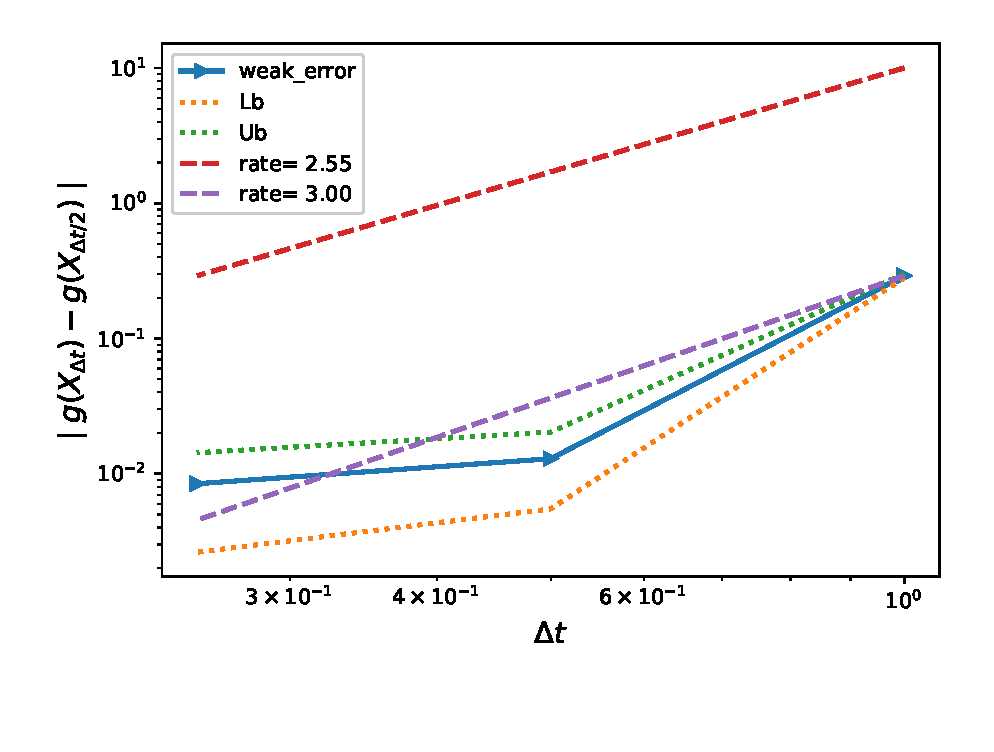
\includegraphics[width=1\linewidth]{./figures/rBergomi_weak_error_rates/with_richardson/H_007/weak_convergence_order_differences_Bergomi_H_007_K_1_richardson_level2_relative_M_10_6_2}
%		\caption{}
%		\label{fig:sub4}
%	\end{subfigure}
%	
%	\caption{The rate of convergence of the weak error for $H=0.07$ $K=1$, with Richardson extraploation (level $2$), using MC with $M=10^6$: a) $\abs{\frac{1}{3}\expt{8 g(X_{\Delta t/4}) -6g(X_{\Delta t/2}) +g(X_{\Delta t})}-g(X)}$  b) $\abs{\frac{1}{3}\expt{-8 g(X_{\Delta t/8}) +14g(X_{\Delta t/4})-7 (X_{\Delta t/2}) +g(X_{\Delta t})}}$} 
%	\label{fig:Weak_rate_H_007_with_rich_level2}
%\end{figure}
%
%
%


\subsection{Comparing different  errors and complexity for MC and MISC}\label{sec:Comparing different  errors and complexity for MC and MISC}


The results were reported for the different sets of parameters defined in table \ref{table:Reference solution, using MC with $500$ time steps, of Call option price under rBergomi model, for different parameter constellation.}. We considered   number of time steps $N \in \{2,4,8,16\}$.  The options are priced in terms of the moneyness $K$, where $K$ is the strike price.   

 For each set,  we report the results for 2 scenarios: i) Without using Richardson extrapolation and  ii) Using level $1$ Richardson extrapoaltion.

In each case, we show a table of computed values using MISC for different tolerances as well biased MC value, using large number of samples to kill the statistical error. Then, in a second table,  we show the bias as well the statistical error for MC method. The third table shows the relative quadrature error which is computed as the normalized difference between the biased MC solution and MISC solution. Then we provide the total relative error which is the sum of the bias and statistical error for MC, and the quadrature error for MISC. Finally, we show the CPU time needed for each solver. We also provide plots for the behavior of Quadrature error of MISC and complexity plots for the different methods. 





%\begin{figure}[!h]
%	\begin{center}
%		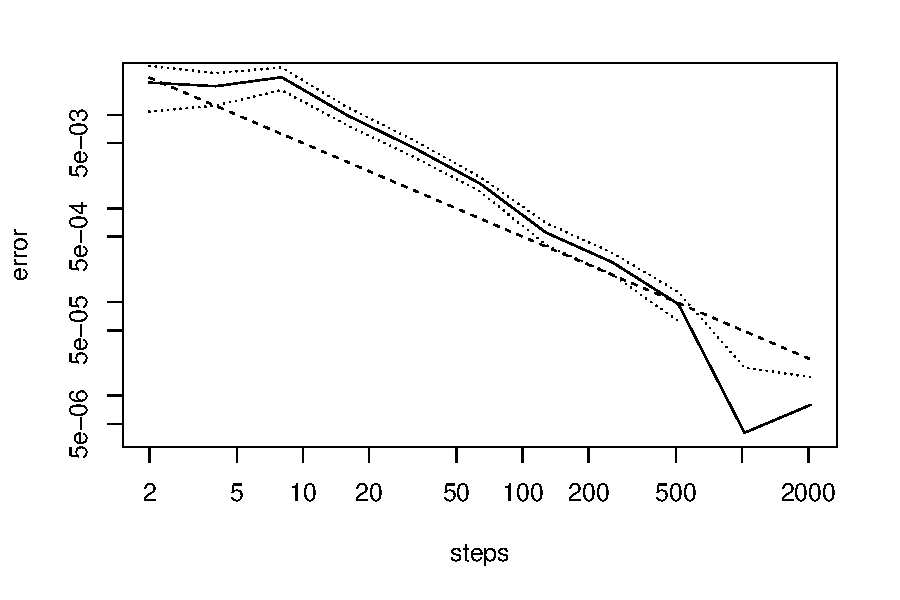
\includegraphics[scale=0.5]{./figures/rBergomi_weak_error/weak_RT.pdf}
%		\caption{The weak error of rBergomi model}
%		\label{fig:rBergomi_weak_error}
%	\end{center}
%\end{figure}

%We note that for some cases, the convergence becomes extremely slow (either the bias stagnates at one value or it keeps increasing or decreasing without reaching the prescribed tolerance) specially when we are close to at-the money option ($K$ close to 1), we do not put values for those cases. We also remark that we have better agreement between the results of MISC coupled with the C++ code and the MC method using the python code form \cite{mccrickerd2017turbocharging}, for small values of moneyness.

%In Section \ref{sec:MISC plots}, we show the convergence plots given by MISC library for the cases of $H=\{0.43,0.07\}$ and $K=0.1$.


%Table \ref{table: Complexity rates for different number of time steps_rbergomi} summarizes the obtained complexity rates for different number of time steps (for more details, see Section \ref{sec:MISC plots}. 
%
%\begin{table}[h!]
%	\centering
%	\begin{tabular}{l*{6}{c}r}
%		Method \textbackslash  Steps             &  $4$ & $8$  & $16$   \\
%		\hline
%		without Richardson  extrapolation(hierarchical) $(H=0.43)$ & $-0.34$ & $-0.33$ & $-0.75$   \\
%		without Richardson  extrapolation (non hierarchical) $(H=0.43)$ & $-0.17$ & $-0.6$ & $-1$   \\
%		without Richardson  extrapolation (hierarchical) $(H=0.07)$ & $-0.64$ & $-0.84$ & $-2.5$   \\
%		without Richardson  extrapolation (total hierarchical) $(H=0.07)$ & $-0.70$ & $-0.88$ & $-2.7$   \\
%		without Richardson  extrapolation (non hierarchical) $(H=0.07)$ & $-0.67$ & $-1.6$ & $-2.9$   \\
%		\hline
%	\end{tabular}
%	\caption{Complexity rates for different number of time steps for $K=1$ and $H=\{0.43,0.07\}$}
%	\label{table: Complexity rates for different number of time steps_rbergomi}
%\end{table}





\subsubsection{Case of set $5$ parameters in table \ref{table:Reference solution, using MC with $500$ time steps, of Call option price under rBergomi model, for different parameter constellation.}}\label{sec:Case of set 5 parameters}

\begin{table}[h!]
	\centering
	\begin{tabular}{l*{6}{c}r}
		Method \textbackslash  Steps            & $2$ & $4$ & $8$ & $16$ &   \\
		\hline
		MISC ($TOl=5.10^{-1}$)  & $0.1258$ & $0.1239$ & $0.1231$ & $0.1227$  \\
		MISC ($TOl=10^{-1}$)  & $0.1258$ & $0.1239$ & $0.1231$ & $0.1229$  \\
		MISC ($TOl=5.10^{-2}$)  & $0.1258$ & $0.1239$ & $0.1231$ & $0.1241$  \\
		MISC ($TOl=10^{-2}$)  & $0.1258$ & $0.1246$ & $0.1248$ & $0.1250$  \\
		
		MISC ($TOl=10^{-3}$)  & $0.1271$ & $0.1259$ & $0.1252$ & $0.1249$  \\
		MISC ($TOl=10^{-4}$)  & $0.1270$ & $0.1258$ & $0.1252$ & $-$  \\
		
			MISC ($TOl=10^{-5}$)  & $0.1270$ &$0.1258$ &  $0.1252$ & $-$  \\
		\hline
		MC method ($M=3.10^{6}$)   & $    0.1269$ & $0.1257$  & $0.1253$ & $0.1249$ \\		
		
		\hline
	\end{tabular}
	\caption{ Call option price of the different methods for different number of time steps. Case of set $5$ parameters in table \ref{table:Reference solution, using MC with $500$ time steps, of Call option price under rBergomi model, for different parameter constellation.}, without Richardson extrapolation.}
	\label{table: Call option price of the different methods for different number of time steps. Case set 5}
\end{table}


\begin{table}[h!]
	\centering
	\begin{tabular}{l*{6}{c}r}
		Method \textbackslash  Steps            & $2$ & $4$ & $8$ & $16$  \\
		\hline
		MC Bias ($M=3.10^6$)   & 	$ \underset{(    0.0022)}{\mathbf{0.0174}}$  & $\underset{(0.001)}{\mathbf{0.0078}}$  & $\underset{(0.0005)}{\mathbf{0.0042}}$ & $\underset{(0.0001)}{\mathbf{0.0008}}$\\ 
		
		MC Statistical error ($M=3.10^6$)  &  $\underset{(   6.2e-05)} {\mathbf{5.0e-04}}$  & $\underset{(5.9e-05)} {\mathbf{4.7e-04}}$  & $\underset{(5.8e-05)} {\mathbf{4.6e-04 }}$ & $\underset{(5.8e-05)} {\mathbf{4.6e-04 }}$	\\
		
		\hline
	\end{tabular}
	\caption{Bias and Statistical errors of MC   for computing Call option price  for different number of time steps. Case set 5, without Richardson extrapolation. The numbers between parentheses are the corresponding absolute errors.}
	\label{Bias and Statistical errors of MC ($M=10^6$)  for computing Call option price  for different number of time steps. Case set 5, without Richardson extrapolation. The numbers between parentheses are the corresponding absolute errors.}
\end{table}



\begin{table}[h!]
	\centering
	\begin{tabular}{l*{6}{c}r}
		Method \textbackslash  Steps            & $2$ & $4$ & $8$ & $16$  \\
		\hline
		MISC ($TOl=5.10^{-1}$)  & $\underset{(   0.0011)}{\mathbf{  0.0088}}$ & $\underset{(
			0.0018)}{\mathbf{ 0.0144}}$ & $\underset{( 0.0022)}{\mathbf{0.0176}}$ & $\underset{(  0.0022)}{\mathbf{ 0.0176}}$  \\
		MISC ($TOl=10^{-1}$)  & $\underset{(   0.0011)}{\mathbf{  0.0088}}$ & $\underset{(
			0.0018)}{\mathbf{ 0.0144}}$& $\underset{( 0.0022)}{\mathbf{0.0176}}$  & $\underset{(  0.0020)}{\mathbf{ 0.0160}}$   \\
		MISC ($TOl=5.10^{-2}$)  &$\underset{(   0.0011)}{\mathbf{  0.0088}}$ & $\underset{(
			0.0018)}{\mathbf{ 0.0144}}$ & $\underset{( 0.0022)}{\mathbf{0.0176}}$  & $\underset{(0.0008)}{\mathbf{0.0064}}$  \\
		MISC ($TOl=10^{-2}$)  & $\underset{(   0.0011)}{\mathbf{  0.0088}}$ & $\underset{(0.0011
			)}{\mathbf{ 0.0088
		}}$ & $\underset{(0.0005)}{\mathbf{ 0.0040
		}}$ & $\underset{0.0001}{\mathbf{\red{0.0008}}}$  \\
		MISC ($TOl=10^{-3}$)  & $\underset{( 0.0002)}{\mathbf{    0.0016}}$ & $\underset{(0.0002
			)}{\mathbf{ 0.0016
		}}$ & $\underset{0.0001}{\mathbf{\red{0.0008}}}$ & $\underset{0.00005}{\mathbf{0.0004}}$ \\
		MISC ($TOl=10^{-4}$)  & $\underset{( 0.0001)}{\mathbf{    \red{0.0008}}}$ & $\underset{0.0001}{\mathbf{\red{0.0008}}}$& $\underset{0.0001}{\mathbf{0.0008}}$ & $\underset{-}{\mathbf{-}}$  \\
		
			MISC ($TOl=10^{-5}$)  & $\underset{( 0.0001)}{\mathbf{    0.0008}}$ & $\underset{0.0001}{\mathbf{0.0008}}$& $\underset{0.0001}{\mathbf{0.0008}}$ & $\underset{-}{\mathbf{-}}$  \\
		
		\hline
		
	\end{tabular}
	\caption{Quadrature error of MISC to compute Call option price of the different tolerances for different number of time steps. Case  set $5$ parameters in table \ref{table:Reference solution, using MC with $500$ time steps, of Call option price under rBergomi model, for different parameter constellation.}, without Richardson extrapolation. The numbers between parentheses are the corresponding absolute errors.}
	\label{Quadrature error of MISC to compute Call option price of the different tolerances for different number of time steps. Case  set $5$ parameters, without Richardson extrapolation. The numbers between parentheses are the corresponding absolute errors.}
\end{table}



	\begin{figure}[h!]
		\centering
		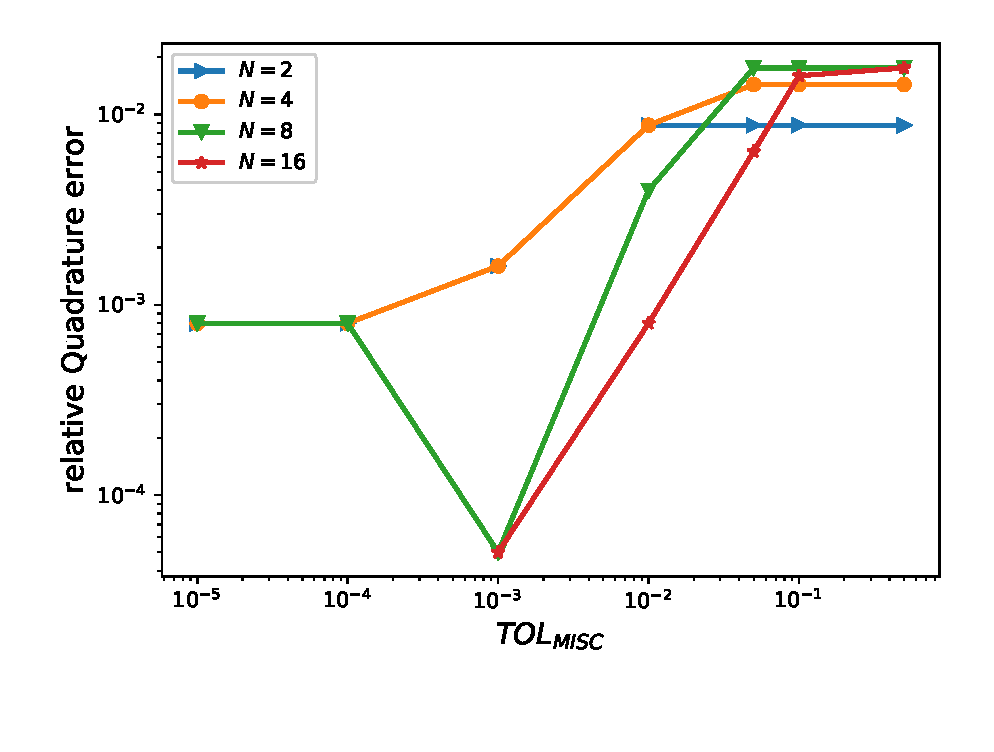
\includegraphics[width=0.7\linewidth]{./figures/rBergomi_MISC_quadratre_error/vs_TOL/set5/relative_quad_error_wrt_MISC_TOL_set5_non_rich}
	
	
	\caption{Quadrature error of MISC to compute Call option price of the different tolerances for different number of time steps. Case  set $5$ parameters, without Richardson extrapolation.}
	\label{fig:Quadrature_error_set5}
\end{figure}




\begin{table}[h!]
	\centering
	\begin{tabular}{l*{6}{c}r}
		Method \textbackslash  Steps            & $2$ & $4$ & $8$ & $16$  \\
		\hline
		MISC ($TOl=5.10^{-1}$)  & $\mathbf{0.0262}$ & $\mathbf{0.0222}$ & $\mathbf{ 0.0218}$ & $\mathbf{ 0.0184}$  \\
		MISC ($TOl=10^{-1}$)  &  $\mathbf{0.0262}$ & $\mathbf{0.0222}$& $\mathbf{ 0.0218}$ & $\mathbf{ 0.0168}$   \\
		MISC ($TOl=5.10^{-2}$)  & $\mathbf{0.0262}$ & $\mathbf{0.0222}$ & $\mathbf{ 0.0218}$ & $\mathbf{ 0.0072}$  \\
		MISC ($TOl=10^{-2}$)  &  $\mathbf{0.0262}$ & $\mathbf{0.0166}$& $\mathbf{ 0.0082}$ & $\mathbf{ \red{0.0016}}$  \\
		MISC ($TOl=10^{-3}$)  &  $\mathbf{0.0190}$ & $\mathbf{0.0094}$& $\mathbf{\red{0.0050}}$  & $\mathbf{ 0.0008}$  \\
		MISC ($TOl=10^{-4}$)  &  $\mathbf{\red{0.0182}}$ & $\mathbf{\red{0.0086}}$& $\mathbf{0.0050}$ & $\mathbf{ -}$ \\
			MISC ($TOl=10^{-5}$)  &  $\mathbf{0.0182}$ & $\mathbf{0.0086}$& $\mathbf{0.0050}$ & $\mathbf{ -}$ 
			 \\
		\hline
		MC    & $\mathbf{\red{0.0179}}$  & $\mathbf{ \red{0.0083}}$  & $\mathbf{\red{0.0047}}$ & $\mathbf{ \red{0.0013}}$  \\		
		\hline
	\end{tabular}
	\caption{Total relative error of MISC and MC to compute Call option price of the different tolerances for different number of time steps. Case Case set $5$ parametrs of table \ref{table:Reference solution, using MC with $500$ time steps, of Call option price under rBergomi model, for different parameter constellation.}, without Richardson extrapolation. The numbers between parentheses are the corresponding absolute errors.}
	\label{Total error of MISC and MC to compute Call option price of the different tolerances for different number of time steps. Case set 5, without Richardson extrapolation. The numbers between parentheses are the corresponding absolute errors.}
\end{table}



\begin{table}[h!]
	\centering
	\begin{tabular}{l*{6}{c}r}
		Method \textbackslash  Steps            & $2$ & $4$ & $8$ & $16$ &   \\
		\hline
		MISC ($TOl=5.10^{-1}$)  & $0.1$ & $0.1$ & $0.2$ & $0.4$  \\
		MISC ($TOl=10^{-1}$)  & $0.1$ & $0.1$ & $0.2$ & $0.8$ \\
		MISC ($TOl=5.10^{-2}$)  & $0.1$ & $0.1$ & $0.2$ & $22$  \\
		MISC ($TOl=10^{-2}$)  & $0.1$ & $0.5$ & $8$ & $\red{92}$ \\
		MISC ($TOl=10^{-3}$)  & $0.5$ & $3$ & $\red{24}$ & $2226$ \\
		MISC ($TOl=10^{-4}$)  & $\red{1}$ & $\red{6}$ & $80$ & $-$\\
		MISC ($TOl=10^{-5}$)  & $2$ & $32$ & $1760$ & $-$
		 \\
		\hline
		MC method   & $ \red{122}
		
		$  & $  \red{211}$  & $  \red{427}$ & $ \red{766}
		$  \\	
		\hline
		Ratio of $\left(MC/MISC \right)$ & $ \red{122}
		
		$  & $  \red{35}$  & $  \red{  18
		}$ & $ \red{ 8}
		$  \\	
		
		\hline
	\end{tabular}
	\caption{Comparsion of the computational time of  MC and MISC, used to compute Call option price of rBergomi model for different number of time steps. Case set $5$ parametrs of table \ref{table:Reference solution, using MC with $500$ time steps, of Call option price under rBergomi model, for different parameter constellation.}. The average  MC CPU time is computed over $10$ runs. }
	\label{Comparsion of the computational time of  MC and MISC, used to compute Call option price of rBergomi model for different number of time steps. Case set5}
\end{table}

	\begin{figure}[h!]
	\centering
	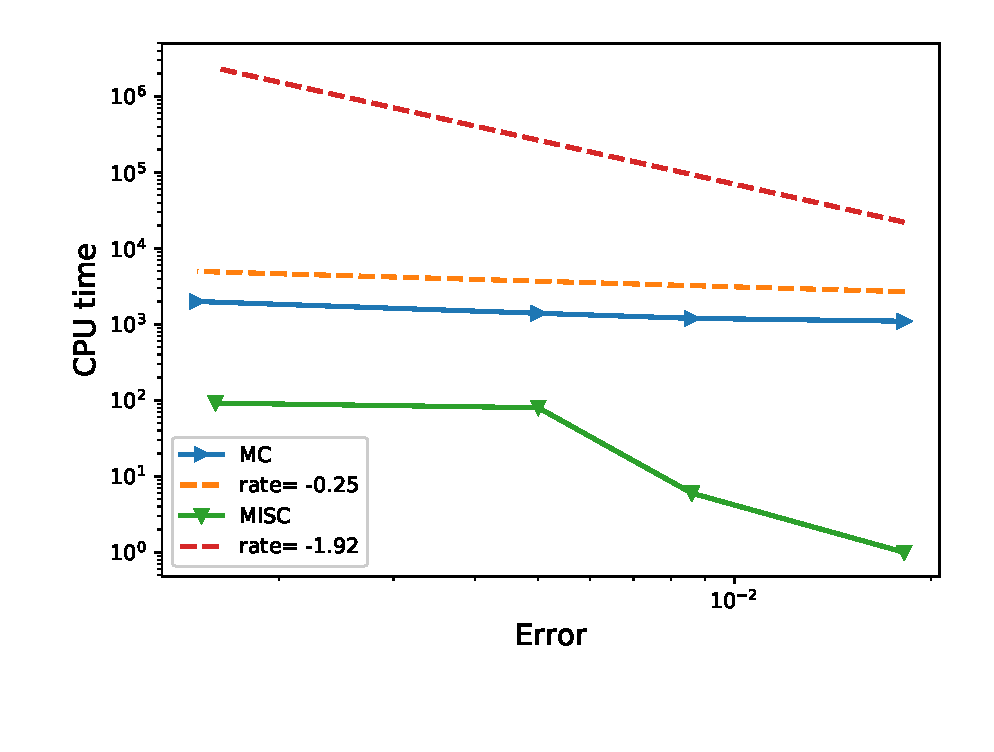
\includegraphics[width=0.7\linewidth]{./figures/rBergomi_Complexity_rates/set5/error_vs_time_set5}

	\caption{Complexity plot for   MC and MISC for Case set $5$ parameters of table \ref{table:Reference solution, using MC with $500$ time steps, of Call option price under rBergomi model, for different parameter constellation.}.}
	\label{fig:Complexity plot for MC and MISC for Case set $5$ parameters}
\end{figure}
\FloatBarrier




\begin{table}[h!]
	\centering
	\begin{tabular}{l*{6}{c}r}
		Method \textbackslash  Steps    &$1-2$         & $2-4$ & $4-8$ & $8-16$\\
		\hline
		MISC ($TOl=5.10^{-1}$)   &$ 0.1261$ & $0.1220$ & $0.1222$ & $0.1223$\\
		MISC ($TOl=10^{-1}$)   &$ 0.1261$ & $0.1220$  &$0.1222$ & $0.1226$\\
		MISC ($TOl=5.10^{-2}$)   &$ 0.1261$ & $0.1220$  & $0.1222$ & $0.1240$ \\
		MISC ($TOl=10^{-2}$)   &$ 0.1267$ & $0.1230$ & $0.1245$ & $0.1247$  \\	
		MISC ($TOl=10^{-3}$)   &$0.1285$ & $0.1247$ & $0.1247$ &  $0.1247$ \\
		MISC ($TOl=10^{-4}$)  &$0.1285$ & $0.1247$ & $0.1247$ & $-$ \\
			MISC ($TOl=10^{-5}$)  &$0.1285$ & $0.1247$ &  $0.1247$ & $-$ \\
	
		\hline
		MC method ($M=10^{7}$)   & $     0.1284$  & $ 
		0.1251$  & $0.1249$ & $  0.1248$ \\		
		\hline
	\end{tabular}
	\caption{Call option price of the different methods for different number of time steps. Case set $5$ parameters of table \ref{table:Reference solution, using MC with $500$ time steps, of Call option price under rBergomi model, for different parameter constellation.}, using Richardson extrapolation (level $1$)}
	\label{table:  Call option price of the different methods for different number of time steps. Case set $5$ parameter, using Richardson extrapolation (level $1$)}
\end{table}



\begin{table}[h!]
	\centering
	\begin{tabular}{l*{6}{c}r}
		Method \textbackslash  Steps            & $1-2$ & $2-4$ & $4-8$ & $8-16$  \\
		\hline
		MC Bias ($M=10^7$)  &$\underset{(  0.0037
			)}{\mathbf{0.0295}}$  & $\underset{( 0.0003)}{\mathbf{0.0025}}$  & $\underset{(   0.0001)}{\mathbf{0.0009}}$  & $\underset{(  6.2e-05)}{\mathbf{0.0005}}$ \\	
		
		MC Statistical error ($M=10^7$)   & $\underset{(  4.4e-05)}{\mathbf{3.5e-04}}$  & $\underset{(   4.2e-05)}{\mathbf{3.4e-04}}$  & $\underset{(  4.1e-05)}{\mathbf{3.3e-04}}$ & $\underset{(  4.1e-05)}{\mathbf{3.3e-04}}$ \\	
		
		
		
		
		
%		MC Statistical error ($M=10^5$)  & $\underset{( 1.3e-03)}{\mathbf{1.6e-02}}$  & $\underset{(   6.9e-04)}{\mathbf{8.7e-03}}$  & $\underset{(  5.0e-04)}{\mathbf{6.3e-03}}$ & $\underset{(  3.9e-04)}{\mathbf{4.9e-03}}$ \\
		\hline
	\end{tabular}
	\caption{Bias and Statistical errors of MC   for computing Call option price  for different number of time steps. Case set $5$ parameters in tabel \ref{table:Reference solution, using MC with $500$ time steps, of Call option price under rBergomi model, for different parameter constellation.}, with Richardson extrapolation (level $1$). The numbers between parentheses are the corresponding absolute errors.}
	\label{Bias and Statistical errors of MC ($M=10^7$)  for computing Call option price  for different number of time steps. Case set $5$ parameters, with Richardson extrapolation (level1). The numbers between parentheses are the corresponding absolute errors.}
\end{table}






\begin{table}[h!]
	\centering
	\begin{tabular}{l*{6}{c}r}
		Method \textbackslash  Steps            & $1-2$ & $2-4$ & $4-8$ & $8-16$  \\
		\hline
		MISC ($TOl=5.10^{-1}$)  & $\underset{(0.0023)}{\mathbf{    0.0184
		}}$  & $\underset{( 0.0031)}{\mathbf{ 0.0248}}$  & $\underset{(   0.0027)}{\mathbf{  0.0216}}$  & $\underset{(
	0.0025
)}{\mathbf{  0.0200}}$  \\ 
		MISC ($TOl=10^{-1}$) & $\underset{(0.0023)}{\mathbf{    0.0184
		}}$  & $\underset{( 0.0031)}{\mathbf{ 0.0248}}$   & $\underset{(   0.0027)}{\mathbf{  0.0216}}$ & $\underset{(  0.0022)}{\mathbf{  0.0176}}$  \\ 
		MISC ($TOl=5.10^{-2}$)  &  $\underset{(0.0023)}{\mathbf{    0.0184
		}}$ & $\underset{( 0.0031)}{\mathbf{ 0.0248}}$   & $\underset{(   0.0027)}{\mathbf{  0.0216}}$  & $\underset{(  0.0008)}{\mathbf{  
		0.0064}}$  \\ 
		MISC ($TOl=10^{-2}$)   & $\underset{(    0.0017
			)}{\mathbf{  0.0136}}$  & $\underset{(
			0.0021)}{\mathbf{   0.0168}}$  & $\underset{(0.0004)}{\mathbf{   0.0032
		}}$  & $\underset{(0.0001)}{\mathbf{\red{0.0008}}}$  \\ 
		MISC ($TOl=10^{-3}$)  & $\underset{(0.0001)}{\mathbf{\red{0.0008}}}$  & $\underset{(0.0006)}{\mathbf{  \red{0.0032}}}$   & $\underset{(0.0002)}{\mathbf{    \red{0.0016}}}$  &  $\underset{(0.0001)}{\mathbf{0.0008}}$  \\ 
		
		MISC ($TOl=10^{-4}$)  & $\underset{(0.0001)}{\mathbf{0.0008}}$  & $\underset{(0.0006)}{\mathbf{ 0.0032}}$   & $\underset{(0.0002)}{\mathbf{   0.0016}}$ & $\underset{(-)}{\mathbf{-}}$  \\

				MISC ($TOl=10^{-5}$)    &  $\underset{(0.0001)}{\mathbf{0.0008}}$ & $\underset{(0.0006)}{\mathbf{  0.0032}}$   & $\underset{(0.0002)}{\mathbf{    0.0016}}$ & $\underset{(-)}{\mathbf{-}}$  \\
		
		\hline
	\end{tabular}
	\caption{Quadrature error of MISC to compute Call option price of the different tolerances for different number of time steps. Case set $5$ parameters in table \ref{table:Reference solution, using MC with $500$ time steps, of Call option price under rBergomi model, for different parameter constellation.}, with Richardson extrapolation(level $1$). The numbers between parentheses are the corresponding absolute errors.}
	\label{Quadrature error of MISC to compute Call option price of the different tolerances for different number of time steps. Case set $5$ parameters, with Richardson extrapolation(level $1$). The numbers between parentheses are the corresponding absolute errors.}
\end{table}


\begin{figure}[h!]
	\centering
	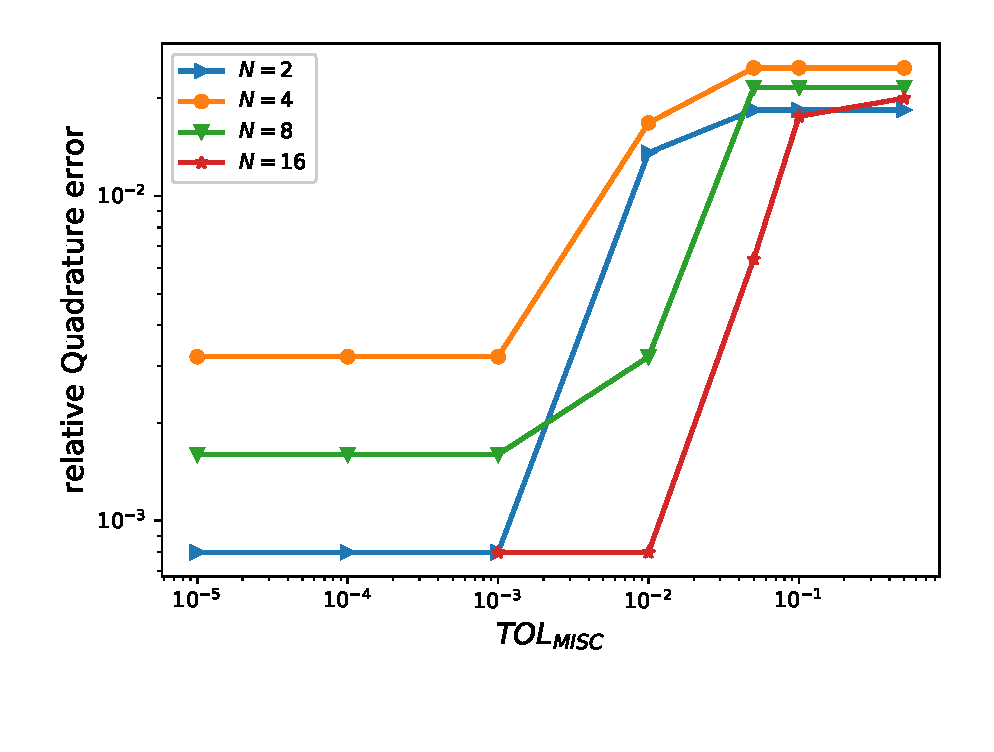
\includegraphics[width=0.7\linewidth]{./figures/rBergomi_MISC_quadratre_error/vs_TOL/set5/relative_quad_error_wrt_MISC_TOL_set5_with_rich}
	
	
	\caption{Quadrature error of MISC to compute Call option price of the different tolerances for different number of time steps. Case  set $5$ parameters, with Richardson extrapolation.}
	\label{fig:Quadrature_error_set5_rich}
\end{figure}

\begin{table}[h!]
	\centering
	\begin{tabular}{l*{6}{c}r}
		Method \textbackslash  Steps            & $1-2$ & $2-4$ & $4-8$ & $8-16$  \\
		\hline
		MISC ($TOl=5.10^{-1}$)  & $0.0479$ & $0.0273$  & $0.0225$ & $0.0205$  \\
		MISC ($TOl=10^{-1}$)   & $0.0479$  &$0.0273$  &$0.0225$ & $0.0181$  \\
		MISC ($TOl=5.10^{-2}$)  &  $0.0479$ & $0.0273$  &$0.0225$ & $0.0069$  \\
			MISC ($TOl=10^{-2}$)  &  $0.0431$ & $0.0193$  & $0.0041$ & $\red{0.0013}$  \\
		MISC ($TOl=10^{-3}$)  & $\red{0.0303}$ & $\red{0.0057}$  & $\red{0.0025}$ & $0.0013$  \\
		MISC ($TOl=10^{-4}$)   & $0.0303$ &$0.0057$  & $0.0033$  & $-$  \\
			MISC ($TOl=10^{-5}$)    &  $0.0303$ &$0.0057$   &  $0.0033$ & $-$  \\	
	\hline

		MC  & $\red{\mathbf{-}}$  & $\red{\mathbf{0.0073}}$  &   $\red{\mathbf{0.0025}}$  &  $\red{\mathbf{0.0013}}$  \\
		\hline
	\end{tabular}
	\caption{Total  error of MISC and MC to compute Call option price of the different tolerances for different number of time steps. Case set $5$ parameters in table \ref{table:Reference solution, using MC with $500$ time steps, of Call option price under rBergomi model, for different parameter constellation.}, with Richardson extrapolation(level $1$). The numbers between parentheses are the corresponding absolute errors.}
	\label{Total  error of MISC and MC to compute Call option price of the different tolerances for different number of time steps. Case set $5$ parameters, with Richardson extrapolation(level $1$). The numbers between parentheses are the corresponding absolute errors.}
\end{table}



\begin{table}[h!]
	\centering
	\begin{tabular}{l*{6}{c}r}
		Method \textbackslash  Steps            & $1-2$ & $2-4$ & $4-8$ & $8-16$ &   \\
		\hline
		MISC ($TOl=5.10^{-1}$)   & $0.08$ & $0.15$ & $0.25$ & $0.5$  \\
		MISC ($TOl=10^{-1}$)   &$0.08$ &  $0.15$ & $0.25$ & $1$  \\
		MISC ($TOl=5.10^{-2}$)  &$0.08$  &  $0.15$ & $0.25$ & $12.5$  \\
		MISC ($TOl=10^{-2}$)   & $0.15$ & $0.6$ & $10$ & $\red{112}$  \\
		MISC ($TOl=10^{-3}$)  & $\red{1}$ & $\red{3.5}$ & $\red{34}$ & $3150$ \\
		MISC ($TOl=10^{-4}$)  & $1$ & $11$ & $328$ & $-$  \\
		MISC ($TOl=10^{-5}$)  & $3$ & $39$ & $2160$ & $-$  \\
		\hline	
			MC method + Richardson (level 1)  &$-$ & $\red{45}$  & $\red{438}$  & $\red{2240}$ \\
			
			\hline
				Ratio of $\left(\text{MC}/ \text{MISC} \right)$  &$-$ & $\red{13}$  & $\red{13}$  & $\red{20}$ \\
%		MC method + Richardson (level 1) ($M=10^{7}$)  &$8363$ & $8974$  & $10308$  & $13166$ \\
		\hline
	\end{tabular}
	\caption{Comparison of the computational time of  MC and MISC, using Richardson extrapolation (level $1$), used to compute Call option price of rBergomi model for different number of time steps. Case set $5$ parameters in table \ref{table:Reference solution, using MC with $500$ time steps, of Call option price under rBergomi model, for different parameter constellation.}. The
average MC CPU time is computed over 10 runs.}
	\label{Comparsion of the computational time of  MC and MISC, using Richardson extrapolation (level $1$), used to compute Call option price of rBergomi model for different number of time steps. Case set $5$ parameters}
\end{table}


\begin{figure}[h!]
	\centering
	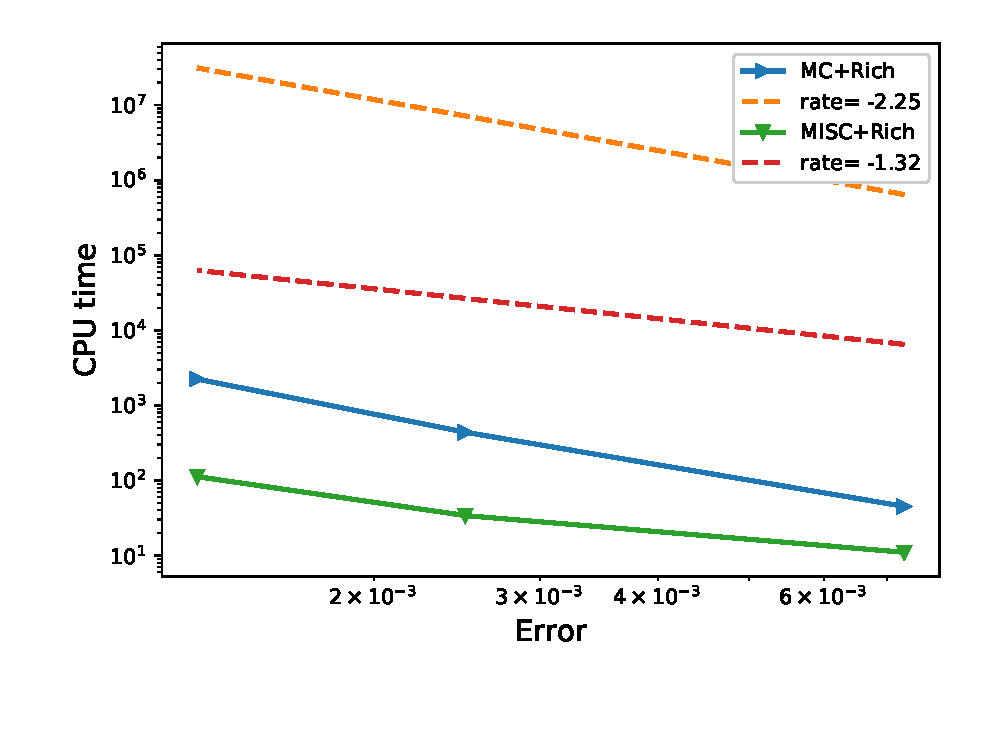
\includegraphics[width=0.7\linewidth]{./figures/rBergomi_Complexity_rates/set5/error_vs_time_set5_rich}
	
	\caption{Complexity plot for  MC and MISC with Richardson extrapolation, for Case set $5$ parameters of table \ref{table:Reference solution, using MC with $500$ time steps, of Call option price under rBergomi model, for different parameter constellation.}.}
	\label{fig:Complexity plot for MC and MISC for Case set $5$ parameters, richardson}
\end{figure}


	\begin{figure}[h!]
	\centering
	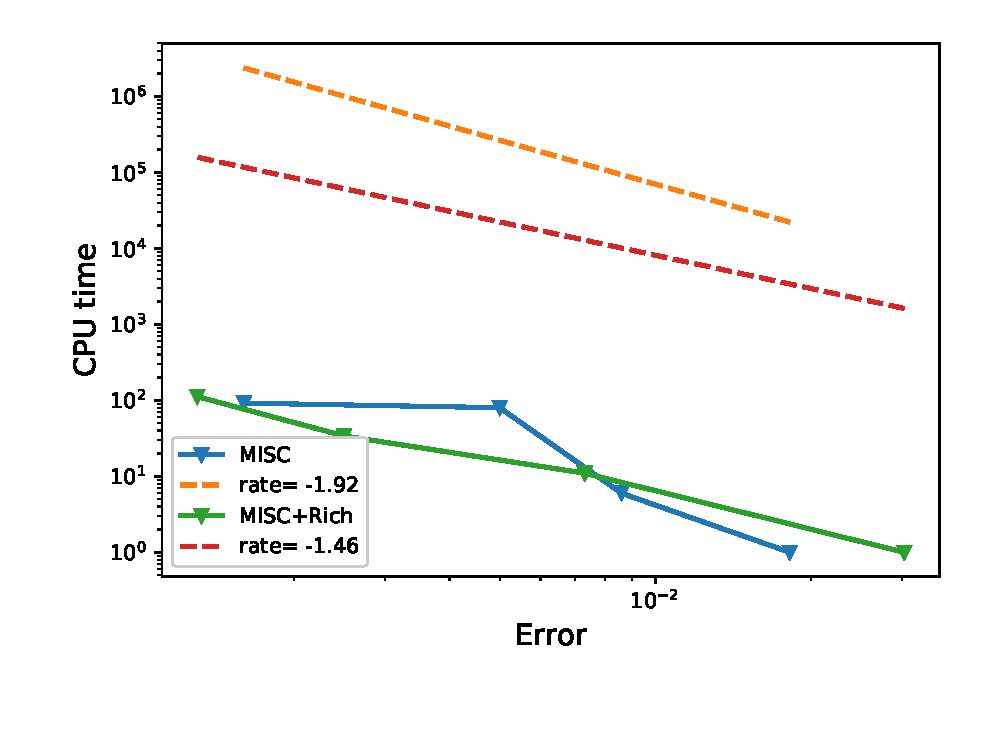
\includegraphics[width=0.7\linewidth]{./figures/rBergomi_Complexity_rates/set5/error_vs_time_set5_comparison}
	
	\caption{Complexity plot for  MISC (with/without) Richardson extrapolation for Case set $5$ parameters of table \ref{table:Reference solution, using MC with $500$ time steps, of Call option price under rBergomi model, for different parameter constellation.}.}
	\label{fig:Complexity plot for  MISC for Case set $5$ parameters, comparison}
\end{figure}





\FloatBarrier




%\subsubsection{Case of set $5$ parameters in table \ref{table:Reference solution, using MC with $500$ time steps, of Call option price under rBergomi model, for different parameter constellation.} with linear hierarchy}
%\label{sec:Case of set $5$ parameters_linear}
%
%\begin{table}[h!]
%	\centering
%	\begin{tabular}{l*{6}{c}r}
%		Method \textbackslash  Steps            & $2$ & $4$ & $8$ & $16$ &   \\
%		\hline
%		MISC ($TOl=5.10^{-1}$)  & $0.1258$ & $0.1239$ & $0.1231$ & $0.1227$  \\
%		MISC ($TOl=10^{-1}$)  & $0.1258$ & $0.1239$ & $0.1231$ & $0.1229$  \\
%		MISC ($TOl=5.10^{-2}$)  & $0.1258$ & $0.1239$ & $0.1231$ & $0.1244$  \\
%		MISC ($TOl=10^{-2}$)  & $0.1258$ & $0.1246$ & $0.1248$ & $0.1250$  \\
%		MISC ($TOl=5.10^{-3}$)  & $0.1258$ & $0.1251$ & $0.1252$ & $0.1251$   \\
%		MISC ($TOl=10^{-3}$)  & $0.1270$ & $0.1259$ & $0.1252$ & $0.1249$  \\
%		MISC ($TOl=10^{-4}$)  & $0.1270$ & $0.1258$ & $0.1252$ & $-$  \\
%	
%		\hline
%		MC method ($M=3.10^{6}$)   & $    0.1269$ & $0.1257$  & $0.1253$ & $0.1249$ \\		
%		
%		\hline
%	\end{tabular}
%	\caption{ Call option price of the different methods for different number of time steps. Case of set $5$ parameters in table \ref{table:Reference solution, using MC with $500$ time steps, of Call option price under rBergomi model, for different parameter constellation.}, without Richardson extrapolation.}
%	\label{table: Call option price of the different methods for different number of time steps. Case set 5,linear}
%\end{table}
%
%
%
%\begin{table}[h!]
%	\centering
%	\begin{tabular}{l*{6}{c}r}
%		Method \textbackslash  Steps            & $2$ & $4$ & $8$ & $16$ &   \\
%		\hline
%		MISC ($TOl=5.10^{-1}$)  & $0.1$ & $0.1$ & $0.2$ & $0.4$  \\
%		MISC ($TOl=10^{-1}$)  & $0.1$ & $0.1$ & $0.2$ & $1$ \\
%		MISC ($TOl=5.10^{-2}$)  & $0.1$ & $0.1$ & $0.2$ & $32$  \\
%		MISC ($TOl=10^{-2}$)  & $0.1$ & $0.6$ & $12$ & $126$ \\
%			MISC ($TOl=5.10^{-3}$)  & $0.1$ & $1$ & $18$ & $149$ \\
%		MISC ($TOl=10^{-3}$)  & $0.5$ & $5$ & $35$ & $2762$ \\
%		MISC ($TOl=10^{-4}$)  & $1$ & $13$ & $241$ & $-$\\
%%		\hline
%%		MC method   & $ \red{682}
%%		
%%		$  & $  \red{721}$  & $  \red{814}$ & $ \red{1125}
%%		$  \\	
%%		\hline
%%		Ratio of $\left(MC/MISC \right)$ & $ \red{682}
%%		
%%		$  & $  \red{ 120}$  & $  \red{  10
%%		}$ & $ \red{ 12}
%%		$  \\	
%%		
%		\hline
%	\end{tabular}
%	\caption{Comparsion of the computational time of  MC and MISC, used to compute Call option price of rBergomi model for different number of time steps. Case set $5$ parametrs of table \ref{table:Reference solution, using MC with $500$ time steps, of Call option price under rBergomi model, for different parameter constellation.}. The average  MC CPU time is computed over $10$ runs. }
%	\label{Comparsion of the computational time of  MC and MISC, used to compute Call option price of rBergomi model for different number of time steps. Case set5,linear}
%\end{table}
%
%
%
%
%
%
%
%\begin{table}[h!]
%	\centering
%	\begin{tabular}{l*{6}{c}r}
%		Method \textbackslash  Steps    &$1-2$         & $2-4$ & $4-8$ & $8-16$\\
%		\hline
%		MISC ($TOl=5.10^{-1}$)   &$ 0.1261$ & $0.1220$ & $0.1222$ & $0.1223$\\
%		MISC ($TOl=10^{-1}$)   &$ 0.1261$ & $0.1220$  &$0.1222$ & $0.1226$\\
%		MISC ($TOl=5.10^{-2}$)   &$ 0.1261$ & $0.1220$  & $0.1222$ & $0.1240$ \\
%		MISC ($TOl=10^{-2}$)   &$ 0.1261$ & $0.1230$ & $0.1243$ & $0.1247$  \\	
%			MISC ($TOl=5.10^{-3}$)   &$ 0.1267$ & $0.1238$ & $0.1245$ & $0.1247$  \\	
%		MISC ($TOl=10^{-3}$)   &$0.1285$ & $0.1247$ & $0.1247$ &  $0.1247$ \\
%		MISC ($TOl=10^{-4}$)  &$0.1284$ & $0.1245$ & $0.1246$ & $-$ \\
%%		MISC ($TOl=10^{-5}$)  &$0.1284$ & $0.1245$ &  $0.1246$ & $-$ \\
%		
%		\hline
%		MC method ($M=10^{7}$)   & $     0.1284$  & $ 
%		0.1251$  & $0.1249$ & $  0.1248$ \\		
%		\hline
%	\end{tabular}
%	\caption{Call option price of the different methods for different number of time steps. Case set $5$ parameters of table \ref{table:Reference solution, using MC with $500$ time steps, of Call option price under rBergomi model, for different parameter constellation.}, using Richardson extrapolation (level $1$)}
%	\label{table:  Call option price of the different methods for different number of time steps. Case set $5$ parameter, using Richardson extrapolation (level $1$),linear}
%\end{table}
%
%
%
%\begin{table}[h!]
%	\centering
%	\begin{tabular}{l*{6}{c}r}
%		Method \textbackslash  Steps            & $1-2$ & $2-4$ & $4-8$ & $8-16$ &   \\
%		\hline
%		MISC ($TOl=5.10^{-1}$)   & $0.1$ & $0.15$ & $0.25$ & $0.7$  \\
%		MISC ($TOl=10^{-1}$)   &$0.1$ &  $0.15$ & $0.25$ & $1.5$  \\
%		MISC ($TOl=5.10^{-2}$)  &$0.1$  &  $0.15$ & $0.25$ & $28$  \\
%		MISC ($TOl=10^{-2}$)   & $0.1$ & $1$ & $12$ & $143$  \\
%			MISC ($TOl=5.10^{-3}$)   & $0.2$ & $2$ & $15$ & $245$  \\
%		MISC ($TOl=10^{-3}$)  & $1$ & $5$ & $42$ & $3386$ \\
%		MISC ($TOl=10^{-4}$)  & $1$ & $16$ & $497$ & $-$  \\
%%		MISC ($TOl=10^{-5}$)  & $3$ & $83$ & $-$ & $-$  \\
%		\hline	
%%		MC method + Richardson (level 1)  &$-$ & $\red{45}$  & $\red{438}$  & $\red{2240}$ \\
%%		
%%		\hline
%%		Ratio of $\left(\text{MC}/ \text{MISC} \right)$  &$-$ & $\red{4}$  & $\red{13}$  & $\red{20}$ \\
%%		%		MC method + Richardson (level 1) ($M=10^{7}$)  &$8363$ & $8974$  & $10308$  & $13166$ \\
%%		\hline
%	\end{tabular}
%	\caption{Comparison of the computational time of  MC and MISC, using Richardson extrapolation (level $1$), used to compute Call option price of rBergomi model for different number of time steps. Case set $5$ parameters in table \ref{table:Reference solution, using MC with $500$ time steps, of Call option price under rBergomi model, for different parameter constellation.}}
%	\label{Comparsion of the computational time of  MC and MISC, using Richardson extrapolation (level $1$), used to compute Call option price of rBergomi model for different number of time steps. Case set $5$ parameters,linear}
%\end{table}

\FloatBarrier
\subsubsection{Case of set $6$ parameters in table \ref{table:Reference solution, using MC with $500$ time steps, of Call option price under rBergomi model, for different parameter constellation.}}\label{sec:Case of set 6 parameters}

\begin{table}[h!]
	\centering
	\begin{tabular}{l*{6}{c}r}
		Method \textbackslash  Steps            & $2$ & $4$ & $8$ & $16$ &   \\
		\hline
		MISC ($TOl=5.10^{-1}$)  & $0.2413$ & $0.2403$ & $0.2403$ & $0.2396$  \\
		MISC ($TOl=10^{-1}$)  & $0.2413$ &$0.2403$& $0.2403$ & $0.2397$   \\
		MISC ($TOl=5.10^{-2}$)  &$0.2413$ & $0.2403$ & $0.2403$ & $0.2406$  \\
		MISC ($TOl=10^{-2}$)  &$0.2413$ & $0.2403$ & $0.2409$ & $0.2413$  \\
		
		MISC ($TOl=10^{-3}$)  & $0.2413$ & $0.2411$ & $0.2414$ & $0.2413$  \\
		MISC ($TOl=10^{-4}$)  &  $0.2421$ & $0.2416$ & $0.2414$ & $-$  \\
		
		MISC ($TOl=10^{-5}$)  & $0.2421$ &$0.2416$ &  $0.2414$ & $-$  \\
		\hline
		MC method ($M=5.10^{6}$)   & $0.2420$ & $0.2416$  & $0.2414$ & $0.2413$ \\		
		
		\hline
	\end{tabular}
	\caption{ Call option price of the different methods for different number of time steps. Case of set $6$ parameters in table \ref{table:Reference solution, using MC with $500$ time steps, of Call option price under rBergomi model, for different parameter constellation.}, without Richardson extrapolation.}
	\label{table: Call option price of the different methods for different number of time steps. Case set 6}
\end{table}


\begin{table}[h!]
	\centering
	\begin{tabular}{l*{6}{c}r}
		Method \textbackslash  Steps            & $2$ & $4$ & $8$ & $16$  \\
		\hline
		MC Bias ($M=5.10^6$)   & 	$ \underset{(    0.0013)}{\mathbf{0.0054}}$  & $\underset{(0.0008)}{\mathbf{0.0035
		}}$  & $\underset{(0.0007)}{\mathbf{0.0029}}$ & $\underset{(0.0006)}{\mathbf{0.0024}}$\\ 
		
		MC Statistical error ($M=5.10^6$)  &  $\underset{(   8.3e-05)} {\mathbf{3.4e-04}}$  & $\underset{(8.1e-05)} {\mathbf{3.4e-04}}$  & $\underset{(8.0e-05)} {\mathbf{3.3e-04 }}$ & $\underset{(8.0e-05)} {\mathbf{3.3e-04}}$	\\
		
		\hline
	\end{tabular}
	\caption{Bias and Statistical errors of MC   for computing Call option price  for different number of time steps. Case set 6, without Richardson extrapolation. The numbers between parentheses are the corresponding absolute errors.}
	\label{Bias and Statistical errors of MC ($M=5.10^6$)  for computing Call option price  for different number of time steps. Case set 6, without Richardson extrapolation. The numbers between parentheses are the corresponding absolute errors.}
\end{table}



\begin{table}[h!]
	\centering
	\begin{tabular}{l*{6}{c}r}
		Method \textbackslash  Steps            & $2$ & $4$ & $8$ & $16$  \\
		\hline
		MISC ($TOl=5.10^{-1}$)  & $\underset{(   0.0007)}{\mathbf{   0.0029}}$ & $\underset{(
			
			0.0013)}{\mathbf{     0.0054}}$ & $\underset{( 
			0.0011)}{\mathbf{   0.0046}}$ & $\underset{(      0.0017)}{\mathbf{     0.0071
		}}$  \\
		MISC ($TOl=10^{-1}$)  & $\underset{(   0.0007)}{\mathbf{   0.0029}}$ & $\underset{(
			
			0.0013)}{\mathbf{     0.0054}}$& $\underset{( 
			0.0011)}{\mathbf{   0.0046}}$  & $\underset{(    0.0016)}{\mathbf{     0.0066
		}}$   \\
		MISC ($TOl=5.10^{-2}$)  &$\underset{(   0.0007)}{\mathbf{   0.0029}}$ & $\underset{(
			
			0.0013)}{\mathbf{     0.0054}}$ & $\underset{( 
			0.0011)}{\mathbf{   0.0046}}$  & $\underset{(0.0008)}{\mathbf{
				0.0033}}$  \\
		MISC ($TOl=10^{-2}$)  & $\underset{(   0.0007)}{\mathbf{   0.0029}}$ &$\underset{(
			
			0.0013)}{\mathbf{     0.0054}}$ & $\underset{(0.0005)}{\mathbf{    0.0021
		}}$ &  $\underset{2.0e-05}{\mathbf{\red{8.3e-05}}}$  \\
		MISC ($TOl=10^{-3}$)  & $\underset{(   0.0007)}{\mathbf{   0.0029}}$ & $\underset{(0.0005
			)}{\mathbf{ 
				0.0021
		}}$ & $\underset{3.0e-05}{\mathbf{\red{1.2e-04}}}$ &  $\underset{2.0e-05}{\mathbf{8.3e-05}}$  \\
		MISC ($TOl=10^{-4}$)  & $\underset{( 0.0001)}{\mathbf{    \red{0.0004}}}$ & $\underset{5.0e-05}{\mathbf{\red{2.1e-04}}}$& $\underset{3.0e-05}{\mathbf{1.2e-04}}$ & $\underset{-}{\mathbf{-}}$  \\
		
		MISC ($TOl=10^{-5}$)  & $\underset{( 0.0001)}{\mathbf{   0.0004}}$ & $\underset{5.0e-05}{\mathbf{2.1e-04}}$& $\underset{3.0e-05}{\mathbf{1.2e-04}}$& $\underset{-}{\mathbf{-}}$  \\
		
		\hline
		
	\end{tabular}
	\caption{Quadrature error of MISC to compute Call option price of the different tolerances for different number of time steps. Case  set $6$ parameters in table \ref{table:Reference solution, using MC with $500$ time steps, of Call option price under rBergomi model, for different parameter constellation.}, without Richardson extrapolation. The numbers between parentheses are the corresponding absolute errors.}
	\label{Quadrature error of MISC to compute Call option price of the different tolerances for different number of time steps. Case  set $6$ parameters, without Richardson extrapolation. The numbers between parentheses are the corresponding absolute errors.}
\end{table}



\begin{figure}[h!]
	\centering
	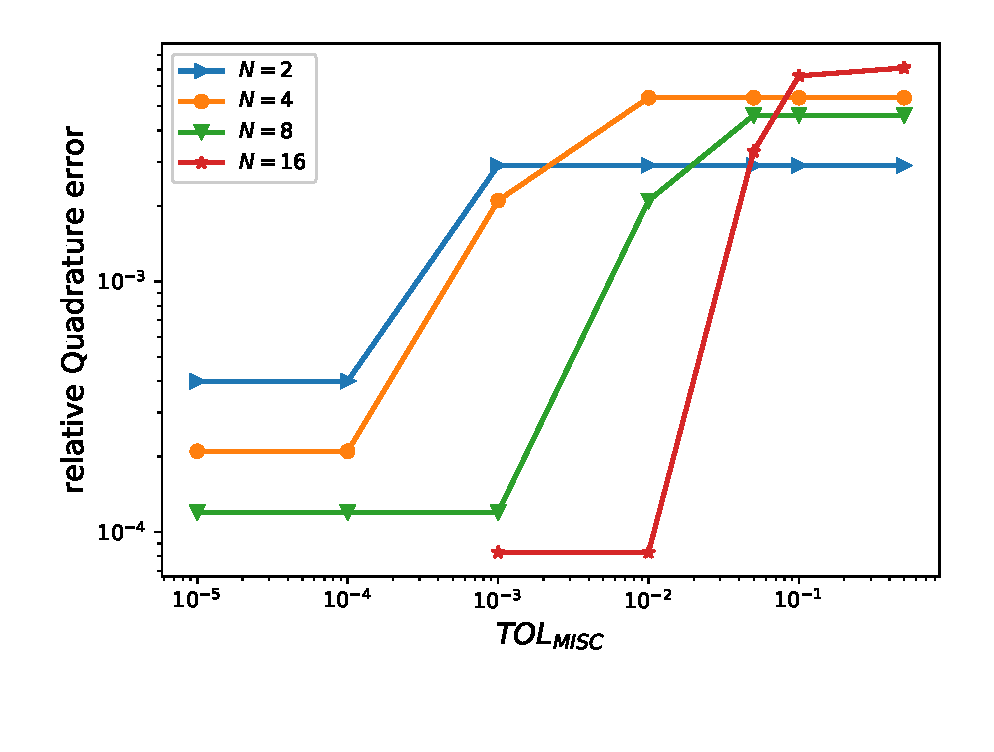
\includegraphics[width=0.7\linewidth]{./figures/rBergomi_MISC_quadratre_error/vs_TOL/set6/relative_quad_error_wrt_MISC_TOL_set6_non_rich}
	
	
	\caption{Quadrature error of MISC to compute Call option price of the different tolerances for different number of time steps. Case  set $6$ parameters, without Richardson extrapolation.}
	\label{fig:Quadrature_error_set6}
\end{figure}





\begin{table}[h!]
	\centering
	\begin{tabular}{l*{6}{c}r}
		Method \textbackslash  Steps            & $2$ & $4$ & $8$ & $16$  \\
		\hline
		MISC ($TOl=5.10^{-1}$)  & $\mathbf{0.0083}$ & $\mathbf{0.0089}$ & $\mathbf{ 0.0075}$ & $\mathbf{ 0.0095}$  \\
		MISC ($TOl=10^{-1}$)  &  $\mathbf{0.0083}$ & $\mathbf{0.0089}$& $\mathbf{ 0.0075}$ & $\mathbf{ 0.0090}$   \\
		MISC ($TOl=5.10^{-2}$)  & $\mathbf{0.0083}$ & $\mathbf{0.0089}$ & $\mathbf{ 0.0075}$ & $\mathbf{ 0.0057}$  \\
		MISC ($TOl=10^{-2}$)  &  $\mathbf{0.0083}$ & $\mathbf{0.0089}$& $\mathbf{ 0.0050}$ & $\mathbf{ \red{0.0025}}$  \\
		MISC ($TOl=10^{-3}$)  &  $\mathbf{0.0083}$& $\mathbf{0.0056}$& $\mathbf{\red{0.0030}}$  & $\mathbf{ 0.0025}$  \\
		MISC ($TOl=10^{-4}$)  &  $\mathbf{\red{0.0058}}$ & $\mathbf{\red{0.0037}}$& $\mathbf{0.0030}$ & $\mathbf{ -}$ \\
		MISC ($TOl=10^{-5}$)  &  $\mathbf{0.0058}$ & $\mathbf{0.0037}$& $\mathbf{0.0030}$ & $\mathbf{ -}$ 
		\\
		\hline
		MC    & $\mathbf{\red{0.0057}}$  & $\mathbf{ \red{0.0038}}$  & $\mathbf{\red{0.0032}}$ & $\mathbf{ \red{0.0027}}$  \\		
		\hline
	\end{tabular}
	\caption{Total relative error of MISC and MC to compute Call option price of the different tolerances for different number of time steps. Case Case set $6$ parametrs of table \ref{table:Reference solution, using MC with $500$ time steps, of Call option price under rBergomi model, for different parameter constellation.}, without Richardson extrapolation. The numbers between parentheses are the corresponding absolute errors.}
	\label{Total error of MISC and MC to compute Call option price of the different tolerances for different number of time steps. Case set 6, without Richardson extrapolation. The numbers between parentheses are the corresponding absolute errors.}
\end{table}


\begin{table}[h!]
	\centering
	\begin{tabular}{l*{6}{c}r}
		Method \textbackslash  Steps            & $2$ & $4$ & $8$ & $16$ &   \\
		\hline
		MISC ($TOl=5.10^{-1}$)  & $0.1$ & $0.1$ & $0.1$ & $0.3$  \\
		MISC ($TOl=10^{-1}$)  & $0.1$ & $0.1$ & $0.1$ & $1$ \\
		MISC ($TOl=5.10^{-2}$)  & $0.1$ & $0.1$ & $0.1$ & $22$  \\
		MISC ($TOl=10^{-2}$)  & $0.1$ & $0.15$ & $9$ & $\red{112}$ \\
		MISC ($TOl=10^{-3}$)  & $0.2$ & $2$ & $\red{27}$ & $2226$ \\
		MISC ($TOl=10^{-4}$)  & $\red{1}$ & $\red{6}$ & $136$ & $-$\\
		MISC ($TOl=10^{-5}$)  & $2$ & $18$ & $1559$ & $-$
		\\
		\hline
		MC method   & $ \red{141}
		
		$  & $  \red{246}$  & $  \red{461}$ & $ \red{820}
		$  \\	
		\hline
		Ratio of $\left(MC/MISC \right)$ & $ \red{141}
		
		$  & $  \red{
			41
		}$  & $  \red{    17
		}$ & $ \red{ 7}
		$  \\	
%		
		\hline
	\end{tabular}
	\caption{Comparsion of the computational time of  MC and MISC, used to compute Call option price of rBergomi model for different number of time steps. Case set $6$ parametrs of table \ref{table:Reference solution, using MC with $500$ time steps, of Call option price under rBergomi model, for different parameter constellation.}. The average  MC CPU time is computed over $10$ runs. }
	\label{Comparsion of the computational time of  MC and MISC, used to compute Call option price of rBergomi model for different number of time steps. Case set6}
\end{table}




	\begin{figure}[h!]
	\centering
	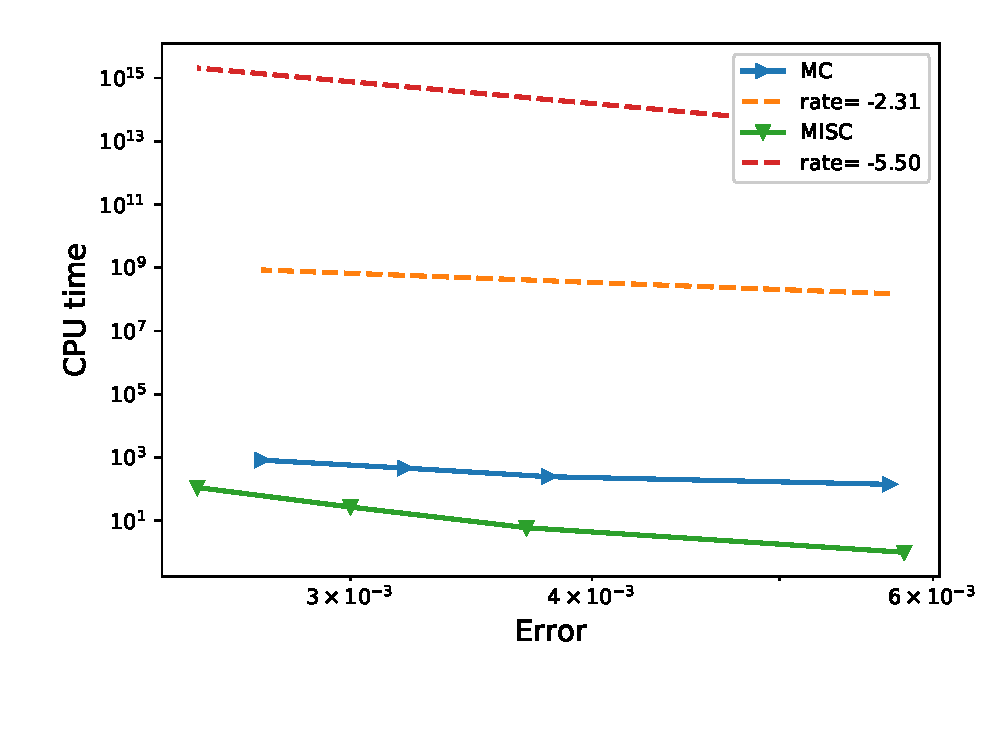
\includegraphics[width=0.7\linewidth]{./figures/rBergomi_Complexity_rates/set6/error_vs_time_set6}
	
	\caption{Complexity plot for   MC and MISC for Case set $6$ parameters of table \ref{table:Reference solution, using MC with $500$ time steps, of Call option price under rBergomi model, for different parameter constellation.}.}
	\label{fig:Complexity plot for MC and MISC for Case set $6$ parameters}
\end{figure}
\FloatBarrier
\subsubsection{Case of set $7$ parameters in table \ref{table:Reference solution, using MC with $500$ time steps, of Call option price under rBergomi model, for different parameter constellation.}}\label{sec:Case of set 7 parameters}

\begin{table}[h!]
	\centering
	\begin{tabular}{l*{6}{c}r}
		Method \textbackslash  Steps            & $2$ & $4$ & $8$ & $16$ &   \\
		\hline
		MISC ($TOl=5.10^{-1}$)  & $0.0590$ & $0.0564$ & $0.0552$ & $0.0546$  \\
		MISC ($TOl=10^{-1}$)  & $0.0590$ &$0.0564$& $0.0552$ & $0.0546$   \\
		MISC ($TOl=5.10^{-2}$)  &$0.0590$ & $0.0564$ & $0.0552$ & $0.0557$  \\
		MISC ($TOl=10^{-2}$)  &$0.0590$ &$0.0564$ & $0.0574$ & $0.0572$  \\
		
		MISC ($TOl=10^{-3}$)  & $0.0605$ & $0.0587$ & $0.0579$ & $0.0575$  \\
		MISC ($TOl=10^{-4}$)  &  $0.0605$ & $0.0587$ & $0.0576$ & $-$  \\
		
		MISC ($TOl=10^{-5}$)  & $0.0605$ & $0.0587$ &  $0.0579$ & $-$  \\
		\hline
		MC method ($M=5.10^{6}$)   & $0.0605$ & $0.0587$  & $0.0579$ & $0.0576$ \\		
		
		\hline
	\end{tabular}
	\caption{ Call option price of the different methods for different number of time steps. Case of set $6$ parameters in table \ref{table:Reference solution, using MC with $500$ time steps, of Call option price under rBergomi model, for different parameter constellation.}, without Richardson extrapolation.}
	\label{table: Call option price of the different methods for different number of time steps. Case set 7}
\end{table}


\begin{table}[h!]
	\centering
	\begin{tabular}{l*{6}{c}r}
		Method \textbackslash  Steps            & $2$ & $4$ & $8$ & $16$  \\
		\hline
		MC Bias ($M=5.10^6$)   & 	$ \underset{(0.0037
			)}{\mathbf{0.0650}}$  & $\underset{(0.0019)}{\mathbf{0.0330
		}}$  & $\underset{(0.0012)}{\mathbf{0.0202}}$ & $\underset{(0.0007)}{\mathbf{0.0130}}$\\ 
		
		MC Statistical error ($M=5.10^6$)  &  $\underset{(   4.0e-05)} {\mathbf{7.0e-04}}$  & $\underset{(3.8e-05)} {\mathbf{6.7e-04}}$  & $\underset{(3.7e-05)} {\mathbf{6.5e-04 }}$ & $\underset{(3.6e-05)} {\mathbf{6.3e-04}}$	\\
		
		\hline
	\end{tabular}
	\caption{Bias and Statistical errors of MC   for computing Call option price  for different number of time steps. Case set 7, without Richardson extrapolation. The numbers between parentheses are the corresponding absolute errors.}
	\label{Bias and Statistical errors of MC ($M=5.10^6$)  for computing Call option price  for different number of time steps. Case set 7, without Richardson extrapolation. The numbers between parentheses are the corresponding absolute errors.}
\end{table}
%
%
%
\begin{table}[h!]
	\centering
	\begin{tabular}{l*{6}{c}r}
		Method \textbackslash  Steps            & $2$ & $4$ & $8$ & $16$  \\
		\hline
		MISC ($TOl=5.10^{-1}$)  & $\underset{(  0.0015
			)}{\mathbf{     0.0264}}$ & $\underset{(    0.0023
			)}{\mathbf{         0.0406}}$ & $\underset{(    0.0028)}{\mathbf{      0.0491
		}}$ & $\underset{(      
	0.0030)}{\mathbf{     0.0524
		}}$  \\
		MISC ($TOl=10^{-1}$)  & $\underset{(  0.0015
			)}{\mathbf{     0.0264}}$& $\underset{(    0.0023
			)}{\mathbf{         0.0406}}$& $\underset{(    0.0028)}{\mathbf{      0.0491
		}}$  & $\underset{(      
	0.0030)}{\mathbf{     0.0524
}}$   \\
		MISC ($TOl=5.10^{-2}$)  &$\underset{(  0.0015
			)}{\mathbf{     0.0264}}$ & $\underset{(    0.0023
			)}{\mathbf{         0.0406}}$ & $\underset{(    0.0028)}{\mathbf{      0.0491
		}}$ & $\underset{(  0.0019)}{\mathbf{
		0.0331
	}}$  \\
		MISC ($TOl=10^{-2}$)  & $\underset{(  0.0015
			)}{\mathbf{     0.0264}}$ &$\underset{(    0.0023
			)}{\mathbf{         0.0406}}$ & $\underset{(0.0005)}{\mathbf{    0.0021
		}}$ &  $\underset{0.0004}{\mathbf{    0.0065}}$  \\
		MISC ($TOl=10^{-3}$)  & $\underset{(      3.0e-05)}{\mathbf{    \red{5.3e-04}}}$ & $\underset{2.0e-05}{\mathbf{\red{3.5e-04}}}$& $\underset{1.9e-05}{\mathbf{\red{3.3e-04}}}$ &  $\underset{3.0e-05}{\mathbf{\red{5.3e-04}}}$  \\
		MISC ($TOl=10^{-4}$)  & $\underset{(      3.0e-05)}{\mathbf{    5.3e-04}}$ & $\underset{2.0e-05}{\mathbf{3.5e-04}}$& $\underset{1.9e-05}{\mathbf{3.3e-04}}$ & $\underset{-}{\mathbf{-}}$  \\
		
		MISC ($TOl=10^{-5}$)  & $\underset{(      3.0e-05)}{\mathbf{    5.3e-04}}$ & $\underset{2.0e-05}{\mathbf{3.5e-04}}$& $\underset{1.9e-05}{\mathbf{3.3e-04}}$& $\underset{-}{\mathbf{-}}$  \\
		
		\hline
		
	\end{tabular}
	\caption{Quadrature error of MISC to compute Call option price of the different tolerances for different number of time steps. Case  set $7$ parameters in table \ref{table:Reference solution, using MC with $500$ time steps, of Call option price under rBergomi model, for different parameter constellation.}, without Richardson extrapolation. The numbers between parentheses are the corresponding absolute errors.}
	\label{Quadrature error of MISC to compute Call option price of the different tolerances for different number of time steps. Case  set $7$ parameters, without Richardson extrapolation. The numbers between parentheses are the corresponding absolute errors.}
\end{table}







\begin{figure}[h!]
	\centering
	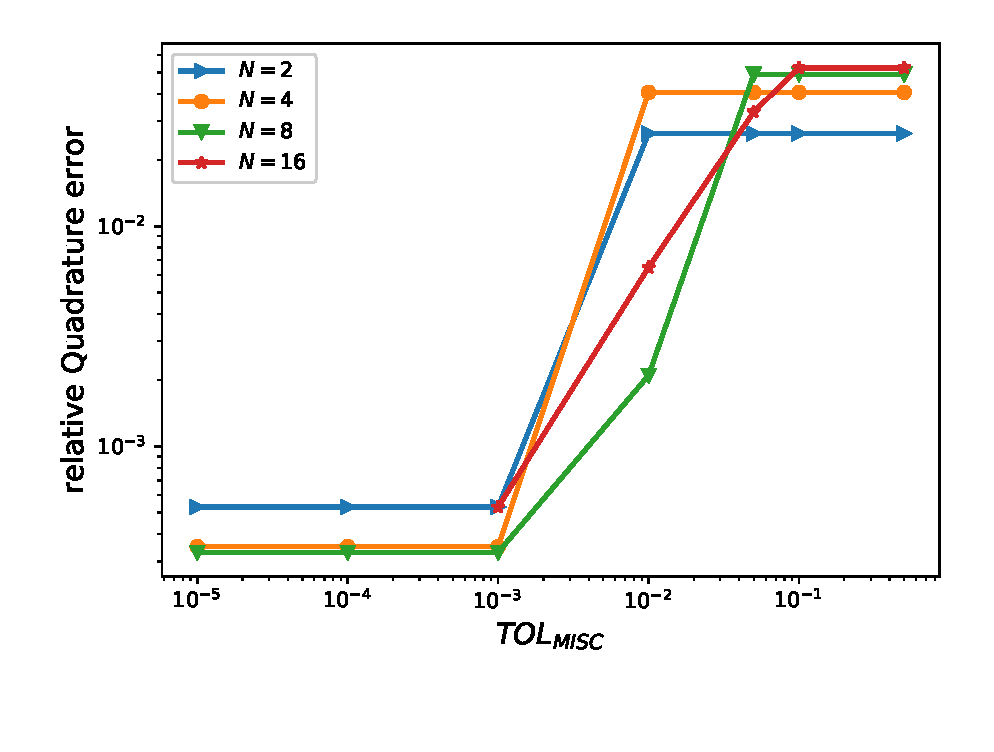
\includegraphics[width=0.7\linewidth]{./figures/rBergomi_MISC_quadratre_error/vs_TOL/set7/relative_quad_error_wrt_MISC_TOL_set7_non_rich}
	
	
	\caption{Quadrature error of MISC to compute Call option price of the different tolerances for different number of time steps. Case  set $7$ parameters, without Richardson extrapolation.}
	\label{fig:Quadrature_error_set7}
\end{figure}


%
%
%
\begin{table}[h!]
	\centering
	\begin{tabular}{l*{6}{c}r}
		Method \textbackslash  Steps            & $2$ & $4$ & $8$ & $16$  \\
		\hline
		MISC ($TOl=5.10^{-1}$)  & $\mathbf{0.0914}$ & $\mathbf{0.0736}$ & $\mathbf{ 0.0693}$ & $\mathbf{ 0.0654}$  \\
		MISC ($TOl=10^{-1}$)  & $\mathbf{0.0914}$ & $\mathbf{0.0736}$& $\mathbf{ 0.0693}$ & $\mathbf{ 0.0654}$   \\
		MISC ($TOl=5.10^{-2}$)  & $\mathbf{0.0914}$ & $\mathbf{0.0736}$ & $\mathbf{ 0.0693}$ & $\mathbf{ 0.0461}$  \\
		MISC ($TOl=10^{-2}$)  &  $\mathbf{0.0914}$& $\mathbf{0.0736}$& $\mathbf{ 0.0223}$ & $\mathbf{ 0.0195}$  \\
		MISC ($TOl=10^{-3}$)  &  $\mathbf{\red{0.0655}}$& $\mathbf{\red{0.0334}}$& $\mathbf{\red{0.0205}}$  & $\mathbf{ \red{0.0135}}$  \\
		MISC ($TOl=10^{-4}$)  &  $\mathbf{0.0655}$& $\mathbf{0.0334}$& $\mathbf{0.0205}$ & $\mathbf{ -}$ \\
		MISC ($TOl=10^{-5}$)  &  $\mathbf{0.0655}$ & $\mathbf{0.0334}$& $\mathbf{0.0205}$ & $\mathbf{ -}$ 
		\\
		\hline
		MC    & $\mathbf{\red{0.0657}}$  & $\mathbf{ \red{0.0337}}$  & $\mathbf{\red{0.0209}}$ & $\mathbf{ \red{0.0136}}$  \\		
		\hline
	\end{tabular}
	\caption{Total relative error of MISC and MC to compute Call option price of the different tolerances for different number of time steps. Case Case set $7$ parametrs of table \ref{table:Reference solution, using MC with $500$ time steps, of Call option price under rBergomi model, for different parameter constellation.}, without Richardson extrapolation. The numbers between parentheses are the corresponding absolute errors.}
	\label{Total error of MISC and MC to compute Call option price of the different tolerances for different number of time steps. Case set 7, without Richardson extrapolation. The numbers between parentheses are the corresponding absolute errors.}
\end{table}


\begin{table}[h!]
	\centering
	\begin{tabular}{l*{6}{c}r}
		Method \textbackslash  Steps            & $2$ & $4$ & $8$ & $16$ &   \\
		\hline
		MISC ($TOl=5.10^{-1}$)  & $0.1$ & $0.1$ & $0.2$ & $0.5$  \\
		MISC ($TOl=10^{-1}$)  & $0.1$ & $0.1$ & $0.2$ & $0.5$ \\
		MISC ($TOl=5.10^{-2}$)  & $0.1$ & $0.1$ & $0.2$ & $5$  \\
		MISC ($TOl=10^{-2}$)  & $0.1$ & $0.1$ & $8$ & $97$ \\
		MISC ($TOl=10^{-3}$)  & $\red{0.7}$ & $\red{4}$ & $\red{26}$ & $\red{1984}$ \\
		MISC ($TOl=10^{-4}$)  & $1$ & $8$ & $173$ & $-$\\
		MISC ($TOl=10^{-5}$)  & $1$ & $32$ & $2129$ & $-$
		\\
		\hline
		MC method   & $ \red{154}
		
		$  & $  \red{229}$  & $  \red{420}$ & $ \red{938}
		$  \\	
		\hline
		Ratio of $\left(MC/MISC \right)$ & $ \red{   220}
		
		$  & $  \red{
		 57
		}$  & $  \red{    16
		}$ & $ \red{ 0.5}
		$  \\	
				
		\hline
	\end{tabular}
	\caption{Comparsion of the computational time of  MC and MISC, used to compute Call option price of rBergomi model for different number of time steps. Case set $7$ parametrs of table \ref{table:Reference solution, using MC with $500$ time steps, of Call option price under rBergomi model, for different parameter constellation.}. The average  MC CPU time is computed over $10$ runs. }
	\label{Comparsion of the computational time of  MC and MISC, used to compute Call option price of rBergomi model for different number of time steps. Case set7}
\end{table}
	\begin{figure}[h!]
	\centering
	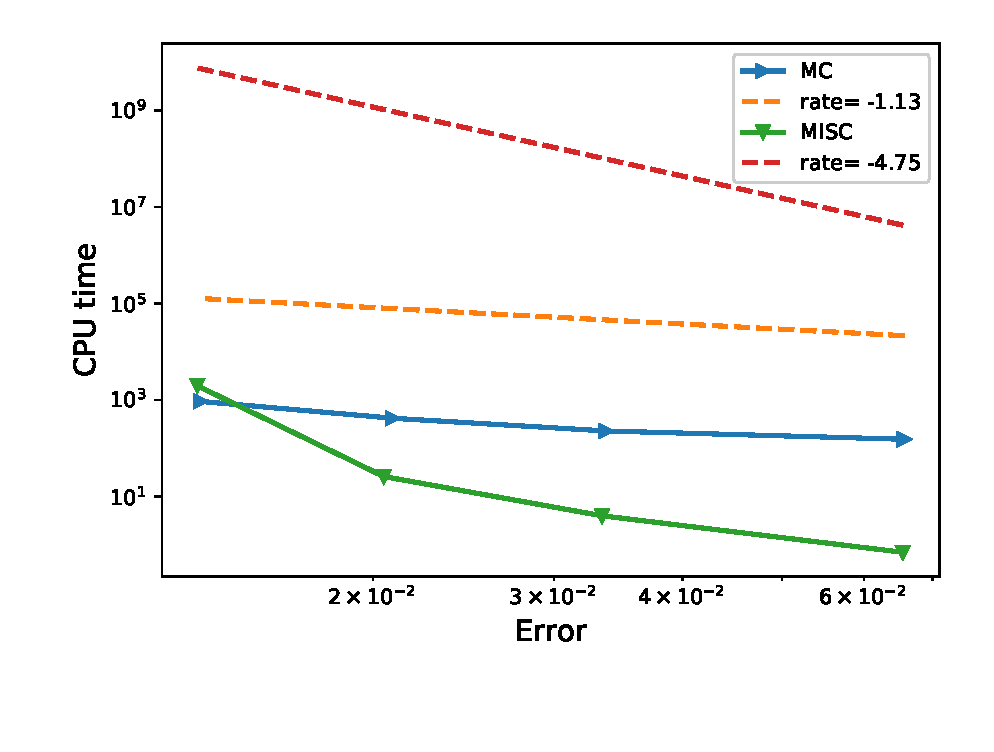
\includegraphics[width=0.7\linewidth]{./figures/rBergomi_Complexity_rates/set7/error_vs_time_set7}
	
	\caption{Complexity plot for   MC and MISC for Case set $5$ parameters of table \ref{table:Reference solution, using MC with $500$ time steps, of Call option price under rBergomi model, for different parameter constellation.}.}
	\label{fig:Complexity plot for MC and MISC for Case set $7$ parameters}
\end{figure}
\FloatBarrier
\subsubsection{Case of set $2$ parameters in table \ref{table:Reference solution, using MC with $500$ time steps, of Call option price under rBergomi model, for different parameter constellation.}}
\label{sec:Case of set $2$ parameters}


\begin{table}[h!]
	\centering
	\begin{tabular}{l*{6}{c}r}
		Method \textbackslash  Steps            & $2$ & $4$ & $8$ & $16$  \\
		\hline
			MISC ($TOl=5.10^{-1}$)  & $0.1082$ & $0.0917$ & $0.0800$ & $0.0732$  \\
		MISC ($TOl=10^{-1}$)  & $0.1082$ & $0.0917$ & $0.0786$ & $0.080$  \\
			MISC ($TOl=5.10^{-2}$)  & $0.1082$ & $0.0921$ & $0.0914$ & $0.0817$  \\
		MISC ($TOl=10^{-2}$)  & $0.1187$ &  $0.1014$ & $0.0909$ & $-$  \\
		MISC ($TOl=10^{-3}$)        & $0.1216$ &$0.1024$ &  $0.0910$ &  $-$ \\
			MISC ($TOl=10^{-4}$)        & $0.1218$ &$0.1024$ &  $-$ &  $-$ \\
	\hline
		MC method ($M=8.10^{6}$)   & $0.1218 $  & $0.1024 $  & $0.0914$ & $0.0850 $ \\		
		\hline
	\end{tabular}
	\caption{ Call option price of the different methods for different number of time steps. Case of set $2$ parameters in table \ref{table:Reference solution, using MC with $500$ time steps, of Call option price under rBergomi model, for different parameter constellation.}, without Richardson extrapolation.}
	\label{table: Call option price of the different methods for different number of time steps. Case set 2}
\end{table}



\begin{table}[h!]
	\centering
	\begin{tabular}{l*{6}{c}r}
		Method \textbackslash  Steps            & $2$ & $4$ & $8$ & $16$  \\
		\hline
		MC Bias ($M=8.10^6$)   & $\underset{(0.0426)}{\mathbf{0.5375
		}}$  & $\underset{ (  0.0208)}{\mathbf{0.2922}}$  & $\underset{(  0.0122)}{\mathbf{0.1542}}$ & $\underset{( 0.0058)}{\mathbf{0.0731}}$  \\	
		
			MC Statistical error ($M=8.10^6$)  & $\underset{( 2.0e-04)}{\mathbf{2.5e-03}}$  & $\underset{(  1.0e-04)}{\mathbf{1.3e-03}}$  & $\underset{(  5.0e-05)}{\mathbf{6.3e-04}}$ & $\underset{(  1.1e-04)}{\mathbf{1.33e-03}}$ \\	
%				MC Statistical error ($M=10^4$)  & $\underset{( 1.6e-03)}{\mathbf{2.0e-02}}$  & $\underset{(  1.5e-03)}{\mathbf{1.9e-02}}$  & $\underset{(  1.1e-03)}{\mathbf{1.4e-02}}$ & $\underset{(  1.0e-03)}{\mathbf{1.3e-02}}$ \\
				
%					MC Statistical error ($M=10^5$)  & $\underset{( 7.7e-04)}{\mathbf{9.7e-03}}$  & $\underset{(  5.1e-04)}{\mathbf{6.5e-03}}$  & $\underset{(  4.7e-04)}{\mathbf{5.9e-03}}$ & $\underset{(  3.2e-04)}{\mathbf{4.0e-03}}$ \\
		\hline
	\end{tabular}
	\caption{Bias and Statistical errors of MC  for computing Call option price  for different number of time steps. Case set $2$ parameters in table \ref{table:Reference solution, using MC with $500$ time steps, of Call option price under rBergomi model, for different parameter constellation.}, without Richardson extrapolation. The numbers between parentheses are the corresponding absolute errors.}
	\label{Bias and Statistical errors of MC ($M=10^6$)  for computing Call option price  for different number of time steps. Case set $2$ parameters, without Richardson extrapolation. The numbers between parentheses are the corresponding absolute errors.}
\end{table}


\begin{table}[h!]
	\centering
	\begin{tabular}{l*{6}{c}r}
		Method \textbackslash  Steps            & $2$ & $4$ & $8$ & $16$  \\
		\hline
		MISC ($TOl=5.10^{-1}$)  & $\underset{(    0.0136)}{\mathbf{    0.1717}}$ & $\underset{(   0.0106)}{\mathbf{   0.1345}}$ & $\underset{(0.0114
			)}{\mathbf{0.1442
		}}$ & $\underset{(0.0118)}{\mathbf{0.1490}}$  \\
		MISC ($TOl=10^{-1}$)  & $\underset{(    0.0136)}{\mathbf{    0.1717}}$ & $\underset{(   0.0106)}{\mathbf{   0.1345}}$ & $\underset{(0.0128)}{\mathbf{0.1619}}$ & $\underset{(0.005)}{\mathbf{0.0631}}$  \\
			MISC ($TOl=5.10^{-2}$)  &$\underset{(    0.0136)}{\mathbf{    0.1717}}$ & $\underset{(   0.0102
				)}{\mathbf{    0.1294}}$ & $\underset{(2.0e-05)}{\mathbf{2.5e-04}}$ & $\underset{(0.0033)}{\mathbf{0.0417}}$  \\
	MISC ($TOl=10^{-2}$)  & $\underset{(    0.0031)}{\mathbf{0.0391
	}}$ & $\underset{(0.001)}{\mathbf{  0.0120}}$ & $\underset{(0.0004)}{\mathbf{\red{0.0066}}}$ & $\underset{-}{\mathbf{-}}$  \\
		MISC ($TOl=10^{-3}$)        & $\underset{(
			1.8e-04)}{\mathbf{   \red{0.0023}
		}}$  &$\underset{(5.0e-05)}{\mathbf{\red{6.3e-04}}}$  &  $\underset{(0.0004)}{\mathbf{0.0053}}$ &  $-$ \\
	MISC ($TOl=10^{-4}$)        & $\underset{(2.0e-05)}{\mathbf{2.5e-04}} $ &$\underset{(5.0e-05)}{\mathbf{6.3e-04}}$ &  $-$ &  $-$ \\	
		
		\hline
	\end{tabular}
	\caption{Quadrature error of MISC to compute Call option price of the different tolerances for different number of time steps. Case  set $2$ parameters in table \ref{table:Reference solution, using MC with $500$ time steps, of Call option price under rBergomi model, for different parameter constellation.}, without Richardson extrapolation. The numbers between parentheses are the corresponding absolute errors.}
	\label{Quadrature error of MISC to compute Call option price of the different tolerances for different number of time steps. Case  set $2$ parameters, without Richardson extrapolation. The numbers between parentheses are the corresponding absolute errors.}
\end{table}





\begin{figure}[h!]
	\centering
	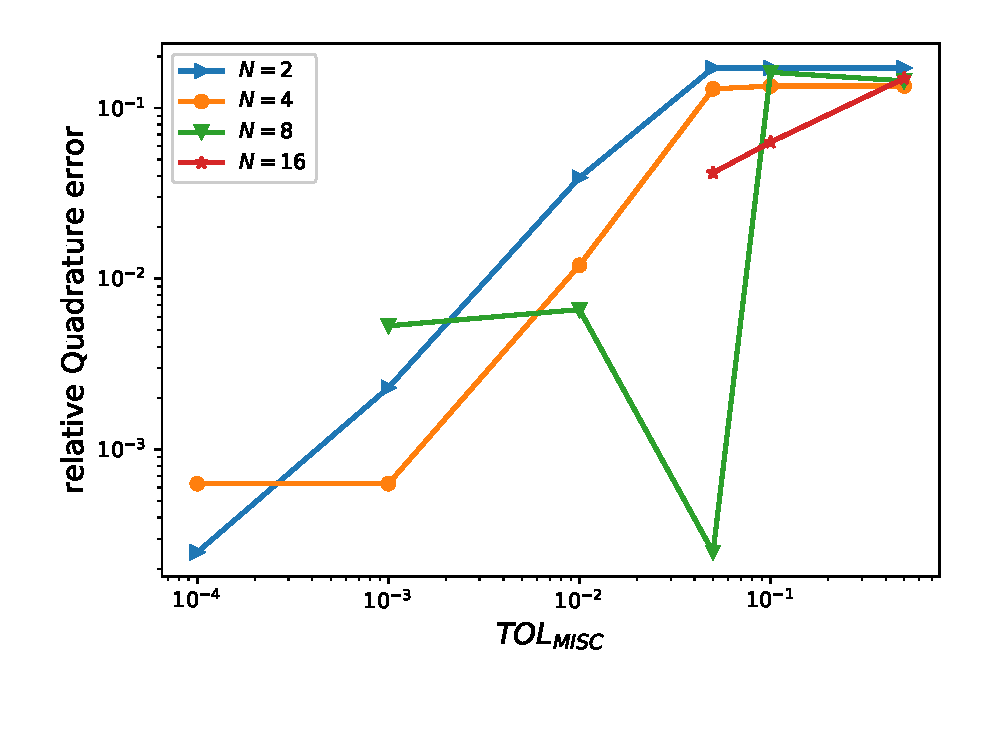
\includegraphics[width=0.7\linewidth]{./figures/rBergomi_MISC_quadratre_error/vs_TOL/set2/relative_quad_error_wrt_MISC_TOL_set2_non_rich}
	
	
	\caption{Quadrature error of MISC to compute Call option price of the different tolerances for different number of time steps. Case  set $2$ parameters, without Richardson extrapolation.}
	\label{fig:Quadrature_error_set2}
\end{figure}



\begin{table}[h!]
	\centering
	\begin{tabular}{l*{6}{c}r}
		Method \textbackslash  Steps            & $2$ & $4$ & $8$ & $16$  \\
		\hline
		MISC ($TOl=5.10^{-1}$)  & $\mathbf{0.7092}$ & $\mathbf{0.4267}$ & $\mathbf{0.2984}$ & $\mathbf{ 0.2221}$  \\
		MISC ($TOl=10^{-1}$)  & $\mathbf{0.7092}$ & $\mathbf{0.4267}$ & $\mathbf{ 0.3161
}$ & $\mathbf{0.1362}$  \\
		MISC ($TOl=5.10^{-2}$)  &$\mathbf{0.7092}$ & $\mathbf{   0.4216
	}$ & $\mathbf{0.1545 }$ & $\mathbf{ 0.1148}$  \\
		MISC ($TOl=10^{-2}$)  & $\mathbf{ 0.5766}$ & $\mathbf{0.2942}$ & $\mathbf{ \red{0.1608} }$ & $\mathbf{-}$  \\
	MISC ($TOl=10^{-3}$)        & $\mathbf{\red{0.5398}}$  &  $\mathbf{\red{0.2928}}$ &  $\mathbf{0.1595}$ &  $-$ \\
		MISC ($TOl=10^{-4}$)        & $\mathbf{0.5378}$  & $\mathbf{0.2928}$  &  $-$ &  $-$ \\
	\hline
	MC    & $\mathbf{\red{0.5400}}$  & $\mathbf{\red{0.2935}
	}$  &$\mathbf{\red{
		0.1593}}$  & $\mathbf{-}$  \\	
%		MC  ($M=10^6$)   & $\mathbf{0.5782}$  & $ \mathbf{  0.2649
%		}$  & $\mathbf{0.1456}$ & $\mathbf{0.0744}$  \\	
%			
%			MC  ($M=10^5$)   & $\mathbf{0.5824}$  & $ \mathbf{  0.2694
%		}$  & $\mathbf{0.1470}$ & $\mathbf{0.0771}$  \\	
%		MC  ($M=10^4$)   & $\mathbf{0.5927}$  & $ \mathbf{  0.2819
%	}$  & $\mathbf{0.1551}$ & $\mathbf{0.0861}$  \\	
		\hline
	\end{tabular}
	\caption{Total error of MISC and MC to compute Call option price of the different tolerances for different number of time steps. Case  set $2$ parameters in table \ref{table:Reference solution, using MC with $500$ time steps, of Call option price under rBergomi model, for different parameter constellation.}, without Richardson extrapolation. The numbers between parentheses are the corresponding absolute errors.}
	\label{Total error of MISC and MC to compute Call option price of the different tolerances for different number of time steps. Case $K=1$, $H=0.07$, without Richardson extrapolation. The numbers between parentheses are the corresponding absolute errors.}
\end{table}



\begin{table}[h!]
	\centering
	\begin{tabular}{l*{6}{c}r}
		Method \textbackslash  Steps            & $2$ & $4$ & $8$ & $16$ &   \\
		\hline
			MISC ($TOl=5.10^{-1}$)  & $0.08$ & $0.13$ & $0.2$ & $0.5$  \\
		MISC ($TOl=10^{-1}$)  & $0.08$ & $0.13$ & $1$ & $220$  \\
		MISC ($TOl=5.10^{-2}$)  & $0.08$ & $0.3$ & $10$ & $5600$  \\
		MISC ($TOl=10^{-2}$)  & $0.45$ & $6$ & $\red{800}$ & $-$  \\
		MISC ($TOl=10^{-3}$)  & $\red{7}$ & $\red{350}$ & $5370$ & $-$  \\		
			MISC ($TOl=10^{-4}$)  & $63$ & $6350$ & $-$ & $-$  \\	
%		MC method ($M=10^4$)   & $0.4$  & $0.4$  & $0.5$ & $0.7$  \\
\hline
		MC method & $\red{220}$  & $\red{358}$  & $\red{9}$ & $-$  \\
		\hline	
		Ratio of $\left(\text{MC}/ \text{MISC} \right)$  &$\red{31.4}$ & $\red{  1
		}$  & $\red { 0.01	}$  & $\red{-}$ \\
		\hline
	\end{tabular}
	\caption{Comparison of the computational time of  MC and MISC, used to compute Call option price of rBergomi model for different number of time steps. Case $K=1, H=0.07$. The
average MC CPU time is computed over 10 runs.}
	\label{Comparsion of the computational time of  MC and MISC, used to compute Call option price of rBergomi model for different number of time steps. Case $K=1, H=0.07$}
\end{table}




%	\begin{figure}[h!]
%	\centering
%	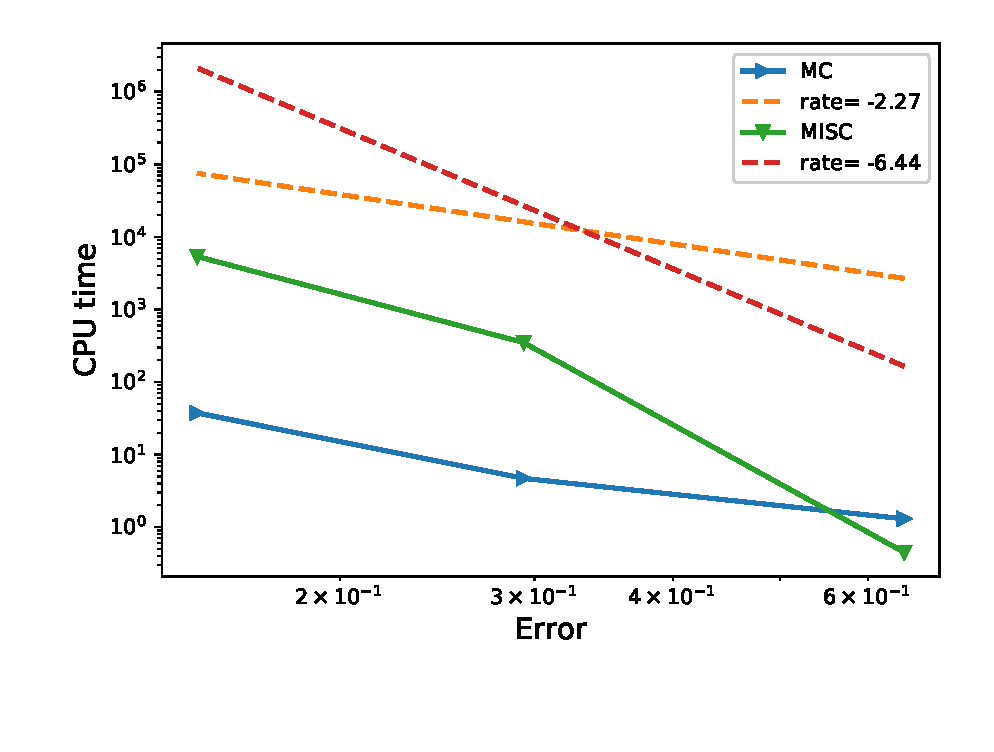
\includegraphics[width=0.7\linewidth]{./figures/rBergomi_Complexity_rates/set2/error_vs_time_set2}
%	
%	\caption{Complexity plot for   MC and MISC for Case set $2$ parameters of table \ref{table:Reference solution, using MC with $500$ time steps, of Call option price under rBergomi model, for different parameter constellation.}.}
%	\label{fig:Complexity plot for MC and MISC for Case set $2$ parameters}
%\end{figure}

\begin{table}[h!]
	\centering
	\begin{tabular}{l*{6}{c}r}
		Method \textbackslash  Steps    &$1-2$         & $2-4$ & $4-8$ & $8-16$\\
		\hline
		MISC ($TOl=5.10^{-1}$)  &$0.1242$ & $0.0752$ & $0.0682$ & $0.0665$ \\
		MISC ($TOl=10^{-1}$)  &$0.1242$ & $0.0752$ & $0.0658$ & $0.0764$  \\
		MISC ($TOl=5.10^{-2}$)   &$0.1242$ & $0.0676$ & $0.0800$ & $-$   \\
		MISC ($TOl=10^{-2}$)  &$0.1459$ & $0.0845$ & $0.0803$ & $-$  \\	
		MISC ($TOl=10^{-3}$)  &$0.1505$ & $0.0827$ & $-$ & $-$ \\
			MISC ($TOl=5.10^{-4}$)  &$0.1505$ & $0.0830$ & $-$ & $-$ \\
		MISC ($TOl=10^{-4}$)  &$0.1500$ & $-$ & $-$ & $-$ \\
		\hline
			MC method ($M=10^{6}$)   & $0.1552 $  & $0.0846 $  & $0.0804$ & $0.0796 $ \\		
		\hline
	\end{tabular}
	\caption{Call option price of the different methods for different number of time steps. Case set $2$ parameters of table \ref{table:Reference solution, using MC with $500$ time steps, of Call option price under rBergomi model, for different parameter constellation.}, using Richardson extrapolation (level $1$)}
	\label{table:  Call option price of the different methods for different number of time steps. Case set $2$ parameter, using Richardson extrapolation (level $1$)}
\end{table}



\begin{table}[h!]
	\centering
	\begin{tabular}{l*{6}{c}r}
		Method \textbackslash  Steps            & $1-2$ & $2-4$ & $4-8$ & $8-16$  \\
		\hline
		MC Bias ($M=10^6$)  &$\underset{( 0.0760)}{\mathbf{0.9594}}$  & $\underset{( 0.0054)}{\mathbf{0.0686}}$  & $\underset{(   0.0012)}{\mathbf{0.0149}}$  & $\underset{(  0.0004)}{\mathbf{0.0048}}$ \\	
		
		MC Statistical error ($M=10^6$)   & $\underset{( 1e-03)}{\mathbf{1.3e-02}}$  & $\underset{(   3.2e-04)}{\mathbf{4.1e-03}}$  & $\underset{(  1.7e-04)}{\mathbf{2.1e-03}}$ & $\underset{(  1.3e-04)}{\mathbf{1.6e-03}}$ \\	
		
		
		
 
			
%			MC Statistical error ($M=10^5$)  & $\underset{( 1.3e-03)}{\mathbf{1.6e-02}}$  & $\underset{(   6.9e-04)}{\mathbf{8.7e-03}}$  & $\underset{(  5.0e-04)}{\mathbf{6.3e-03}}$ & $\underset{(  3.9e-04)}{\mathbf{4.9e-03}}$ \\
		\hline
	\end{tabular}
	\caption{Bias and Statistical errors of MC   for computing Call option price  for different number of time steps. Case set $2$ parameters in tabel \ref{table:Reference solution, using MC with $500$ time steps, of Call option price under rBergomi model, for different parameter constellation.}, with Richardson extrapolation (level $1$). The numbers between parentheses are the corresponding absolute errors.}
	\label{Bias and Statistical errors of MC ($M=10^6$)  for computing Call option price  for different number of time steps. Case set $2$ parameters, with Richardson extrapolation (level1). The numbers between parentheses are the corresponding absolute errors.}
\end{table}



\begin{table}[h!]
	\centering
	\begin{tabular}{l*{6}{c}r}
		Method \textbackslash  Steps            & $1-2$ & $2-4$ & $4-8$ & $8-16$  \\
		\hline
			MISC ($TOl=5.10^{-1}$)  & $\underset{0.0310}{\mathbf{0.3914}}$ & $\underset{0.0094}{\mathbf{0.1187}}$ & $\underset{0.0122}{\mathbf{0.1540}}$ & $\underset{0.0131}{\mathbf{0.1654}}$ \\
		MISC ($TOl=10^{-1}$)  & $\underset{0.0310}{\mathbf{0.3914}}$ & $\underset{0.0094}{\mathbf{0.1187}}$ & $\underset{0.0146}{\mathbf{0.1843}}$ & $\underset{0.0032}{\mathbf{0.0404}}$  \\
				MISC ($TOl=5.10^{-2}$)  & $\underset{0.0310}{\mathbf{0.3914}}$ & $\underset{0.0170}{\mathbf{0.2146}}$ & $\underset{0.0004}{\mathbf{0.0050}}$ & $\underset{-}{\mathbf{-}}$  \\
		MISC ($TOl=10^{-2}$)  & $\underset{ 0.0093}{\mathbf{0.1174}}$ & $\underset{0.0001}{\mathbf{0.0013}}$ & $\underset{0.0001}{\mathbf{\red{0.0013}}}$ & $\underset{-}{\mathbf{ -}}$  \\
		MISC ($TOl=10^{-3}$)  & $\underset{  0.0047}{\mathbf{ \red{0.0593}
		}}$ & $\underset{ 0.0019}{\mathbf{ \red{0.0240}}}$ & $\underset{-}{\mathbf{-}}$ & $\underset{-}{\mathbf{-}}$  \\
			MISC ($TOl=5.10^{-4}$)  & $\underset{  0.0047}{\mathbf{ 0.0593
	}}$ & $\underset{    0.0016}{\mathbf{ 0.0202}}$ & $\underset{-}{\mathbf{-}}$ & $\underset{-}{\mathbf{-}}$  \\
		MISC ($TOl=10^{-4}$)  & $\underset{  0.0052}{\mathbf{ 0.0657
	}}$ & $\underset{-}{\mathbf{-}}$ & $\underset{-}{\mathbf{-}}$ & $\underset{-}{\mathbf{-}}$  \\
		%%		MISC ($TOl=5.10^{-2}$)        & $0.3662$ &$-$ &  $-$ &  $-$ \\
		%		MISC ($TOl=10^{-2}$)    & $-$ & $-$  & $-$ & $-$  \\	
		
		\hline
	\end{tabular}
	\caption{Quadrature error of MISC to compute Call option price of the different tolerances for different number of time steps. Case set $2$ parameters in table \ref{table:Reference solution, using MC with $500$ time steps, of Call option price under rBergomi model, for different parameter constellation.}, with Richardson extrapolation(level $1$). The numbers between parentheses are the corresponding absolute errors.}
	\label{Quadrature error of MISC to compute Call option price of the different tolerances for different number of time steps. Case set $2$ parameters, with Richardson extrapolation(level $1$). The numbers between parentheses are the corresponding absolute errors.}
\end{table}




\begin{figure}[h!]
	\centering
	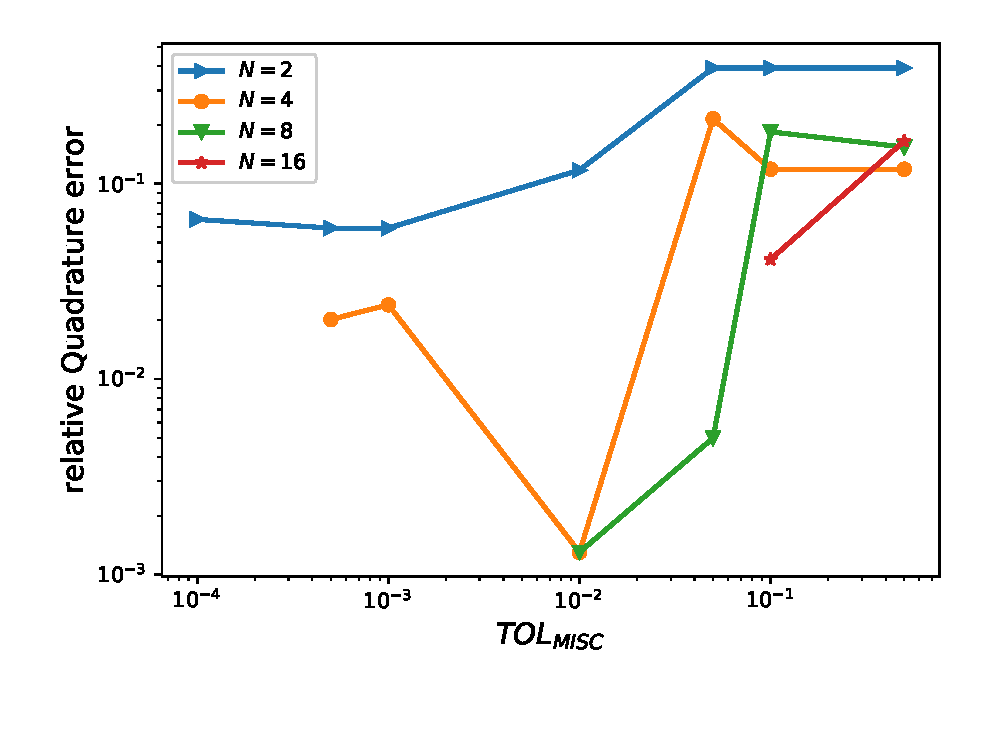
\includegraphics[width=0.7\linewidth]{./figures/rBergomi_MISC_quadratre_error/vs_TOL/set2/relative_quad_error_wrt_MISC_TOL_set2_with_rich}
	
	
	\caption{Quadrature error of MISC to compute Call option price of the different tolerances for different number of time steps. Case  set $2$ parameters, with Richardson extrapolation.}
	\label{fig:Quadrature_error_set2_rich}
\end{figure}

\begin{table}[h!]
	\centering
	\begin{tabular}{l*{6}{c}r}
		Method \textbackslash  Steps            & $1-2$ & $2-4$ & $4-8$ & $8-16$  \\
		\hline
		MISC ($TOl=5.10^{-1}$)  & $\mathbf{1.3508}$ & $\mathbf{  0.1873}$ & $\mathbf{
				0.1689}$ & $\mathbf{ 0.1702}$ \\
		MISC ($TOl=10^{-1}$)  & $\mathbf{1.3508}$ & $\mathbf{0.1873}$ & $\mathbf{0.1992}$ & $\mathbf{0.0458}$  \\
		MISC ($TOl=5.10^{-2}$)  & $\mathbf{1.3508}$ & $\mathbf{0.2832}$ & $\mathbf{0.0199}$ & $\mathbf{-}$  \\
		MISC ($TOl=10^{-2}$)  & $\mathbf{ 1.0768
		}$ & $\mathbf{0.0699}$ & $\mathbf{\red{0.0162}}$ & $\mathbf{-}$  \\
	MISC ($TOl=10^{-3}$)  & $\mathbf{ \red{1.0187}}$ & $\mathbf{\red{0.0926}}$ & $\mathbf{-}$ & $\mathbf{-}$  \\
			MISC ($TOl=5.10^{-4}$)  & $\mathbf{1.0187}$ & $\mathbf{0.0888}$ & $\mathbf{-}$ & $\mathbf{-}$  \\
		MISC ($TOl=10^{-4}$)  & $\mathbf{ 1.0251}$ & $\mathbf{-}$ & $\mathbf{-}$ & $\mathbf{-}$  \\
		%%		MISC ($TOl=5.10^{-2}$)        & $0.3662$ &$-$ &  $-$ &  $-$ \\
		%		MISC ($TOl=10^{-2}$)    & $-$ & $-$  & $-$ & $-$  \\	
		\hline
		
			MC &$\mathbf{ \red{1.0187}}$  & $\mathbf{\red{0.0926}}$ & $\mathbf{\red{0.0162}}$ & $\mathbf{\red{-}}$ \\
%			MC ($M=10^6$) &$\mathbf{0.9724}$  & $\mathbf{0.0727}$  & $\mathbf{0.0170}$  & $\mathbf{0.0064}$ \\	
%%			MC ($M=10^4$) &$\mathbf{1.0284}$  & $\mathbf{0.0876}$  & $\mathbf{0.0329}$  & $\mathbf{0.0198}$ \\
%				MC ($M=10^5$) &$\mathbf{0.9754}$  & $\mathbf{0.0773}$  & $\mathbf{0.0212}$  & $\mathbf{0.0097}$ \\
		\hline
	\end{tabular}
	\caption{Total  error of MISC and MC to compute Call option price of the different tolerances for different number of time steps. Case set $2$ parameters in table \ref{table:Reference solution, using MC with $500$ time steps, of Call option price under rBergomi model, for different parameter constellation.}, with Richardson extrapolation(level $1$). The numbers between parentheses are the corresponding absolute errors.}
	\label{Total  error of MISC and MC to compute Call option price of the different tolerances for different number of time steps. Case set $2$ parameters, with Richardson extrapolation(level $1$). The numbers between parentheses are the corresponding absolute errors.}
\end{table}

\begin{table}[h!]
	\centering
	\begin{tabular}{l*{6}{c}r}
		Method \textbackslash  Steps            & $1-2$ & $2-4$ & $4-8$ & $8-16$ &   \\
		\hline
			MISC ($TOl=5.10^{-1}$)  & $0.1$ & $0.13$ & $0.2$ & $0.5$  \\
		MISC ($TOl=10^{-1}$)  & $0.1$ & $0.13$ & $1.3$ & $1198$  \\
			MISC ($TOl=5.10^{-2}$)  & $0.1$ & $0.5$ & $34$ & $-$  \\
		MISC ($TOl=10^{-2}$)  & $2$ & $9$ & $\red{3450}$ & $-$  \\
			MISC ($TOl=10^{-3}$)  & $\red{16}$ & $\red{2460}$ & $-$ & $-$  \\
			
				MISC ($TOl=5.10^{-4}$)  & $52$ & $9566$ & $-$ & $-$  \\
				MISC ($TOl=10^{-4}$)  & $180$ & $-$ & $-$ & $-$  \\
		\hline	
			MC method + Richardson (level 1)  &$\red{16}$ & $\red{20}$  & $\red{2780}$  & $\red{-}$ \\
%		MC method + Richardson (level 1) ($M=10^{6}$)  &$43$ & $46$  & $54$  & $71$ \\	
%			MC ($M=10^6$) method + Richardson (level 1) ($M=10^{6}$)  &$0.6$ & $0.7$  & $0.8$  & $0.8$ \\	
			
%			MC method + Richardson (level 1) ($M=10^{5}$)  &$5$ & $5$  & $6$  & $8$ \\
\hline	
	Ratio of $\left(\text{MC}/ \text{MISC} \right)$  &$\red{1}$ & $\red{    0.008
	}$  & $\red{ 0.81
}$  & $\red{-}$ \\
		\hline
	\end{tabular}
	\caption{Comparison of the computational time of  MC and MISC, using Richardson extrapolation (level $1$), used to compute Call option price of rBergomi model for different number of time steps. Case set $2$ parameters in table \ref{table:Reference solution, using MC with $500$ time steps, of Call option price under rBergomi model, for different parameter constellation.}. The
average MC CPU time is computed over 10 runs.}
	\label{Comparsion of the computational time of  MC and MISC, using Richardson extrapolation (level $1$), used to compute Call option price of rBergomi model for different number of time steps. Case set $2$ parameters}
\end{table}






\begin{figure}[h!]
	\centering
	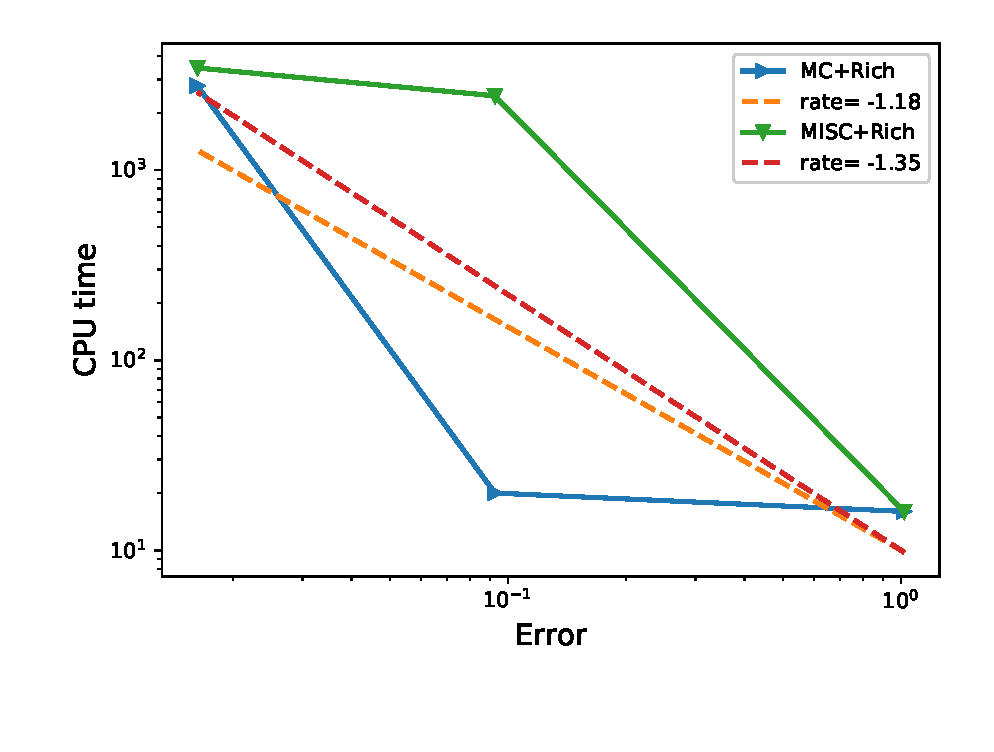
\includegraphics[width=0.7\linewidth]{./figures/rBergomi_Complexity_rates/set2/error_vs_time_set2_rich}
	
	\caption{Complexity plot for  MC and MISC with Richardson extrapolation, for Case set $2$ parameters of table \ref{table:Reference solution, using MC with $500$ time steps, of Call option price under rBergomi model, for different parameter constellation.}.}
	\label{fig:Complexity plot for MC and MISC for Case set $2$ parameters, richardson}
\end{figure}


\begin{figure}[h!]
	\centering
	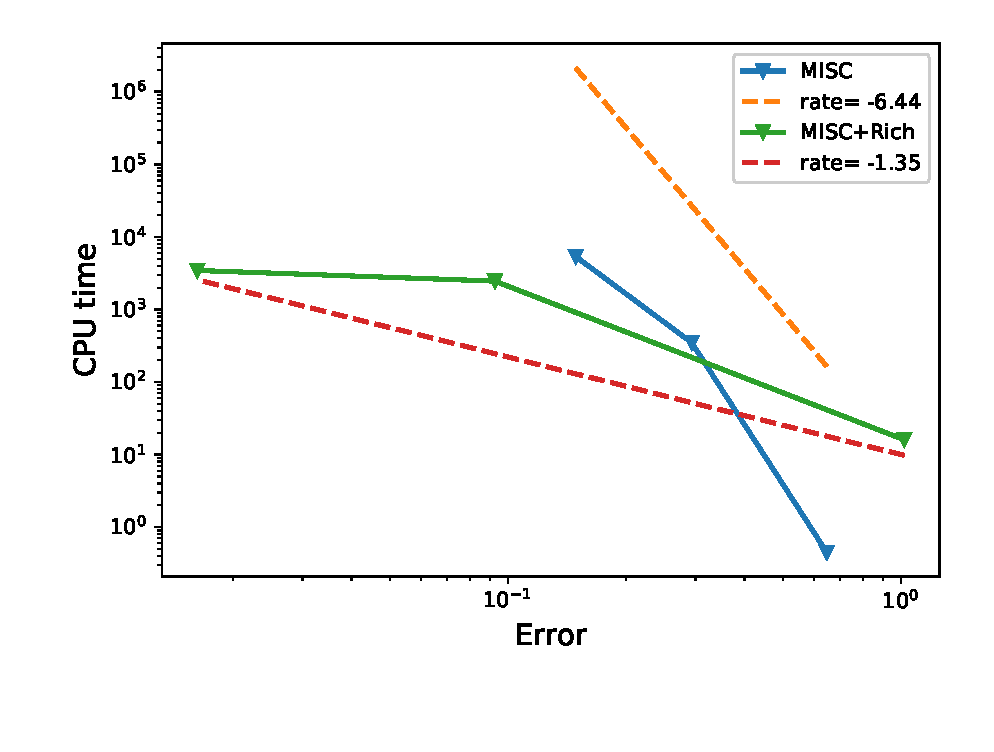
\includegraphics[width=0.7\linewidth]{./figures/rBergomi_Complexity_rates/set2/error_vs_time_set2_comparison}
	
	\caption{Complexity plot for  MISC (with/without) Richardson extrapolation for Case set $2$ parameters of table \ref{table:Reference solution, using MC with $500$ time steps, of Call option price under rBergomi model, for different parameter constellation.}.}
	\label{fig:Complexity plot for  MISC for Case set $2$ parameters, comparison}
\end{figure}

\FloatBarrier



\subsubsection{Case of set $2$ parameters in table \ref{table:Reference solution, using MC with $500$ time steps, of Call option price under rBergomi model, for different parameter constellation.} with linear hierarchy}
\label{sec:Case of set $2$ parameters_linear}


\begin{table}[h!]
	\centering
	\begin{tabular}{l*{6}{c}r}
		Method \textbackslash  Steps            & $2$ & $4$ & $8$ & $16$  \\
		\hline
		MISC ($TOl=5.10^{-1}$)  & $0.1097$ & $0.0926$ & $0.0807$ & $0.0738$  \\
		MISC ($TOl=10^{-1}$)  &$0.1097$ & $0.0926$ & $0.0791$ & $0.0884$  \\
		MISC ($TOl=5.10^{-2}$)  & $0.1097$ & $0.0890$ & $0.0849$ & $0.0842$  \\
		MISC ($TOl=10^{-2}$)  & $0.1119$&  $0.1023$ & $0.0910$ & $0.0842$ \\
		MISC ($TOl=10^{-3}$)        & $0.1195$ &$0.1023$ &   $0.0910$ &  $-$ \\
		MISC ($TOl=10^{-4}$)        & $0.1218$ &$0.1023$ &  $-$ &  $-$ \\
		\hline
		MC method ($M=8.10^{6}$)   & $0.1218 $  & $0.1024 $  & $0.0914$ & $0.0850 $ \\		
		\hline
	\end{tabular}
	\caption{ Call option price of the different methods for different number of time steps. Case of set $2$ parameters in table \ref{table:Reference solution, using MC with $500$ time steps, of Call option price under rBergomi model, for different parameter constellation.}, without Richardson extrapolation.}
	\label{table: Call option price of the different methods for different number of time steps. Case set 2_linear}
\end{table}


\begin{table}[h!]
	\centering
	\begin{tabular}{l*{6}{c}r}
		Method \textbackslash  Steps            & $2$ & $4$ & $8$ & $16$  \\
		\hline
		MISC ($TOl=5.10^{-1}$)  & $\underset{(     0.0121)}{\mathbf{
				 0.1525}}$ & $\underset{(    0.0097)}{\mathbf{      0.1231
			}}$ & $\underset{(   0.0107)}{\mathbf{0.1353
		}}$ & $\underset{(  0.0112)}{\mathbf{0.1414}}$  \\
		MISC ($TOl=10^{-1}$)  & $\underset{(     0.0121)}{\mathbf{
				0.1525}}$ & $\underset{(    0.0097)}{\mathbf{      0.1231
			}}$ & $\underset{( 0.0123
		
			)}{\mathbf{    0.1555}}$ & $\underset{(0.0034)}{\mathbf{0.0429}}$  \\
		MISC ($TOl=5.10^{-2}$)  &$\underset{(     0.0121)}{\mathbf{
				0.1525}}$& $\underset{(     0.0134
			)}{\mathbf{  
				0.1686}}$ & $\underset{(   0.0065)}{\mathbf{ 0.0823}}$ & $\underset{(0.0008)}{\mathbf{
				\red{0.0101}}}$  \\
		MISC ($TOl=10^{-2}$)  & $\underset{(    0.0099
			)}{\mathbf{     0.1247
		}}$ & $\underset{(   5.0e-05)}{\mathbf{\red{  6.3e-04}
	}}$ & $\underset{(0.0004)}{\mathbf{\red{0.0053}}}$ & $\underset{(0.0008)}{\mathbf{0.0101}}$  \\
		MISC ($TOl=10^{-3}$)        & $\underset{(    
			0.0023)}{\mathbf{0.0288}}$  &$\underset{(   5.0e-05)}{\mathbf{  6.3e-04
		}}$ & $\underset{(0.0004)}{\mathbf{0.0053}}$ &  $-$ \\
		MISC ($TOl=10^{-4}$)        & $\underset{(2.0e-05)}{\mathbf{  \red{ 2.5e-04}}} $ &$\underset{(   5.0e-05)}{\mathbf{ 6.3e-04
		}}$ &  $-$ &  $-$ \\	
		
		\hline
	\end{tabular}
	\caption{Quadrature error of MISC to compute Call option price of the different tolerances for different number of time steps. Case  set $2$ parameters in table \ref{table:Reference solution, using MC with $500$ time steps, of Call option price under rBergomi model, for different parameter constellation.}, without Richardson extrapolation. The numbers between parentheses are the corresponding absolute errors.}
	\label{Quadrature error of MISC to compute Call option price of the different tolerances for different number of time steps. Case  set $2$ parameters, without Richardson extrapolation. The numbers between parentheses are the corresponding absolute errors,linear}
\end{table}



\begin{figure}[h!]
	\centering
	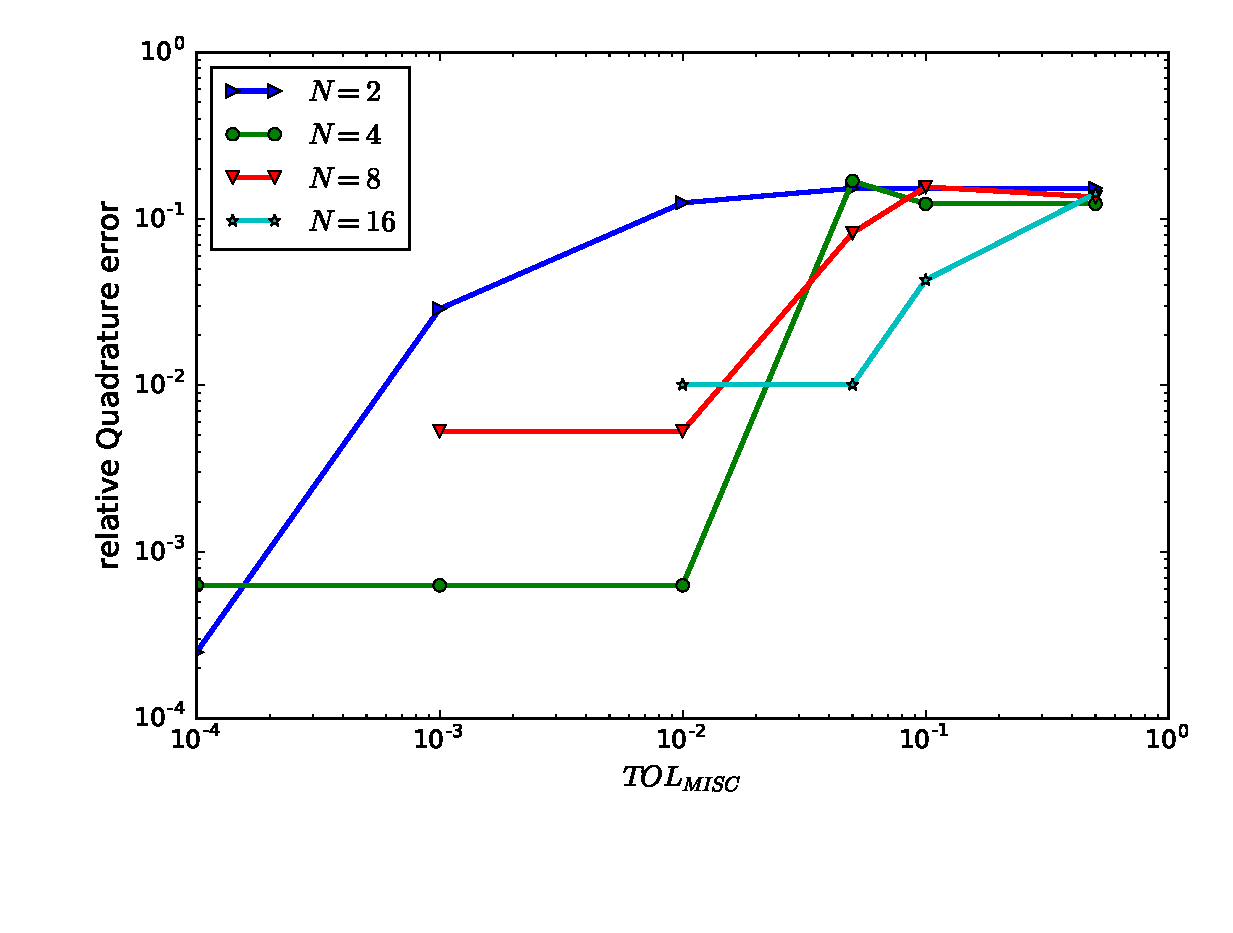
\includegraphics[width=0.7\linewidth]{./figures/rBergomi_MISC_quadratre_error/vs_TOL/set2/relative_quad_error_wrt_MISC_TOL_set2_non_rich_linear}
	
	
	\caption{Quadrature error of MISC to compute Call option price of the different tolerances for different number of time steps. Case  set $2$ parameters, without Richardson extrapolation.}
	\label{fig:Quadrature_error_set2_linear}
\end{figure}

\FloatBarrier
\begin{table}[h!]
	\centering
	\begin{tabular}{l*{6}{c}r}
		Method \textbackslash  Steps            & $2$ & $4$ & $8$ & $16$  \\
		\hline
		MISC ($TOl=5.10^{-1}$)  & $\mathbf{
			0.6900}$ & $\mathbf{   
			0.4153
		}$ & $\mathbf{    0.2895}$ & $\mathbf{     0.2145}$  \\
		MISC ($TOl=10^{-1}$)  & $\mathbf{
			0.6900}$& $\mathbf{    
		0.4153}$ & $\mathbf{     
		0.3097
		}$ & $\mathbf{
		0.1160}$  \\
		MISC ($TOl=5.10^{-2}$)  &$\mathbf{
			0.6900}$ & $\mathbf{         0.4608
	}$ & $\mathbf{      
	0.2365
}$ & $\mathbf{ \red{
		0.0832}}$  \\
		MISC ($TOl=10^{-2}$)  & $\mathbf{ 
			0.6622}$ & $\mathbf{  \red{ 
				0.2928
			}
		}$ & $\mathbf{ \red{    0.1595}}$ & $\mathbf{ 
		0.0832}$  \\
		MISC ($TOl=10^{-3}$)        & $\mathbf{
			0.6371}$  &  $\mathbf{
		0.2928
	}$ &  $\mathbf{    0.1595}$ &  $-$ \\
		MISC ($TOl=10^{-4}$)        & $\mathbf{       \red{0.5378}}$  & $\mathbf{
			0.2928
		}$  &  $-$ &  $-$ \\
		\hline
		MC    & $\mathbf{\red{    0.5400}}$  & $\mathbf{\red{0.2935}
		}$  &$\mathbf{\red{
			0.1593}}$  & $\mathbf{-}$  \\	
	
		\hline
	\end{tabular}
	\caption{Total error of MISC and MC to compute Call option price of the different tolerances for different number of time steps. Case  set $2$ parameters in table \ref{table:Reference solution, using MC with $500$ time steps, of Call option price under rBergomi model, for different parameter constellation.}, without Richardson extrapolation. The numbers between parentheses are the corresponding absolute errors.}
	\label{Total error of MISC and MC to compute Call option price of the different tolerances for different number of time steps. Case $K=1$, $H=0.07$, without Richardson extrapolation. The numbers between parentheses are the corresponding absolute errors,linear}
\end{table}

\begin{table}[h!]
	\centering
	\begin{tabular}{l*{6}{c}r}
		Method \textbackslash  Steps            & $2$ & $4$ & $8$ & $16$ &   \\
		\hline
		MISC ($TOl=5.10^{-1}$)  & $0.08$ & $0.13$ & $0.2$ & $0.5$  \\
		MISC ($TOl=10^{-1}$)  & $0.08$ & $0.13$ & $0.7$ & $163$  \\
		MISC ($TOl=5.10^{-2}$)  & $0.08$ & $0.25$ & $7$ & $\red{1602}$  \\
		MISC ($TOl=10^{-2}$)  & $0.2$& $\red{5}$ & $\red{333}$ & $15082$  \\
		MISC ($TOl=10^{-3}$)  &  $2$ & $73$ & $3650$ & $-$  \\		
		MISC ($TOl=10^{-4}$)  & $\red{43}$ & $1240$ & $-$ & $-$  \\	
		%		MC method ($M=10^4$)   & $0.4$  & $0.4$  & $0.5$ & $0.7$  \\
		\hline
		MC method & $\red{220}$  & $\red{358}$  & $\red{9}$ & $-$  \\
		\hline	
		Ratio of $\left(\text{MC}/ \text{MISC} \right)$  &$\red{5}$ & $\red{   72 
		}$  & $\red {  0.03	}$  & $\red{-}$ \\
		\hline
	\end{tabular}
	\caption{Comparison of the computational time of  MC and MISC, used to compute Call option price of rBergomi model for different number of time steps. Case $K=1, H=0.07$. The
average MC CPU time is computed over 10 runs.}
	\label{Comparsion of the computational time of  MC and MISC, used to compute Call option price of rBergomi model for different number of time steps. Case $K=1, H=0.07$, linear}
\end{table}


\begin{table}[h!]
	\centering
	\begin{tabular}{l*{6}{c}r}
		Method \textbackslash  Steps    &$1-2$         & $2-4$ & $4-8$ & $8-16$\\
		\hline
		MISC ($TOl=5.10^{-1}$)  &$0.1260$ & $0.0756$ & $0.0687$ & $0.0670$ \\
		MISC ($TOl=10^{-1}$)  &$0.1260$ & $0.0756$ & $0.0702$ & $0.0755$  \\
		MISC ($TOl=5.10^{-2}$)   &$0.1260$ & $0.0716$ & $0.0796$ &$0.0755$   \\
		MISC ($TOl=10^{-2}$)  &$0.1456$ & $0.0838$ & $0.0796$ & $-$  \\	
		MISC ($TOl=10^{-3}$)  &$0.1497$ & $0.0838$ & $-$ & $-$ \\

		MISC ($TOl=10^{-4}$)  &$0.1501$ & $-$ & $-$ & $-$ \\
		\hline
		MC method ($M=10^{6}$)   & $0.1552 $  & $0.0846 $  & $0.0804$ & $0.0796 $ \\		
		\hline
	\end{tabular}
	\caption{Call option price of the different methods for different number of time steps. Case set $2$ parameters of table \ref{table:Reference solution, using MC with $500$ time steps, of Call option price under rBergomi model, for different parameter constellation.}, using Richardson extrapolation (level $1$)}
	\label{table:  Call option price of the different methods for different number of time steps. Case set $2$ parameter, using Richardson extrapolation (level $1$),linear}
\end{table}




\begin{table}[h!]
	\centering
	\begin{tabular}{l*{6}{c}r}
		Method \textbackslash  Steps            & $1-2$ & $2-4$ & $4-8$ & $8-16$  \\
		\hline
		MISC ($TOl=5.10^{-1}$)  & $\underset{ 0.0292}{\mathbf{
				0.3687}}$ & $\underset{ 0.0090}{\mathbf{    0.1136}}$ & $\underset{    0.0117
			}{\mathbf{
				0.1477
			}}$ & $\underset{
		0.0126}{\mathbf{ 0.1591}}$ \\
		MISC ($TOl=10^{-1}$)  & $\underset{ 0.0292}{\mathbf{
				0.3687}}$ & $\underset{ 0.0090}{\mathbf{    0.1136}}$ & $\underset{  0.0102}{\mathbf{  0.1288
			}}$ & $\underset{0.0041}{\mathbf{0.0518
		}}$  \\
		MISC ($TOl=5.10^{-2}$)  & $\underset{ 0.0292}{\mathbf{
				0.3687}}$& $\underset{  0.0130}{\mathbf{
				0.1641
			}}$ & $\underset{0.0008}{\mathbf{\red{0.0101}}}$ & $\underset{0.0041}{\mathbf{0.0518
		}}$  \\
		MISC ($TOl=10^{-2}$)  & $\underset{   0.0096
		}{\mathbf{    0.1212
		}}$ & $\underset{0.0008}{\mathbf{
		\red{0.0101}}}$ & $\underset{0.0008 }{\mathbf{
			0.0101}}$ & $\underset{-}{\mathbf{ -}}$  \\
		MISC ($TOl=10^{-3}$)  & $\underset{     0.0055
		}{\mathbf{ \red{    0.0694}
		}}$ & $\underset{0.0008}{\mathbf{
		0.0101}}$ & $\underset{-}{\mathbf{-}}$ & $\underset{-}{\mathbf{-}}$  \\
	
		MISC ($TOl=10^{-4}$)  & $\underset{  0.0051}{\mathbf{    0.0644		}}$ & $\underset{-}{\mathbf{-}}$ & $\underset{-}{\mathbf{-}}$ & $\underset{-}{\mathbf{-}}$  \\
	
		\hline
	\end{tabular}
	\caption{Quadrature error of MISC to compute Call option price of the different tolerances for different number of time steps. Case set $2$ parameters in table \ref{table:Reference solution, using MC with $500$ time steps, of Call option price under rBergomi model, for different parameter constellation.}, with Richardson extrapolation(level $1$). The numbers between parentheses are the corresponding absolute errors.}
	\label{Quadrature error of MISC to compute Call option price of the different tolerances for different number of time steps. Case set $2$ parameters, with Richardson extrapolation(level $1$). The numbers between parentheses are the corresponding absolute errors,linear}
\end{table}




\begin{figure}[h!]
	\centering
	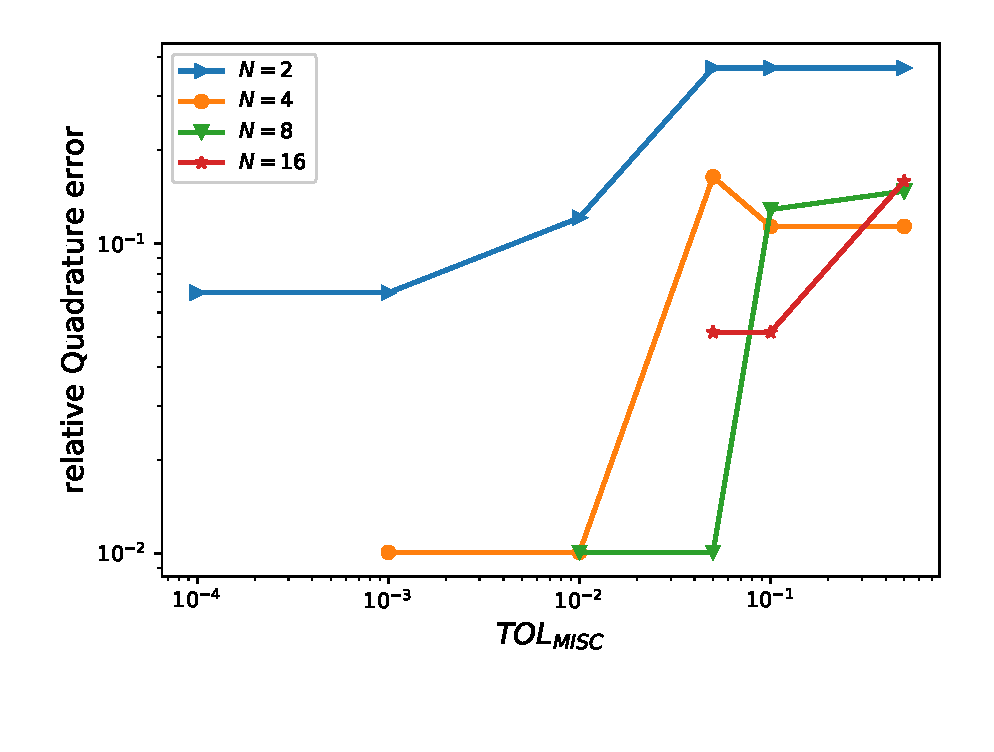
\includegraphics[width=0.7\linewidth]{./figures/rBergomi_MISC_quadratre_error/vs_TOL/set2/relative_quad_error_wrt_MISC_TOL_set2_with_rich_linear}
	
	
	\caption{Quadrature error of MISC to compute Call option price of the different tolerances for different number of time steps. Case  set $2$ parameters, with Richardson extrapolation.}
	\label{fig:Quadrature_error_set2_linear_rich}
\end{figure}


\begin{table}[h!]
	\centering
	\begin{tabular}{l*{6}{c}r}
		Method \textbackslash  Steps            & $1-2$ & $2-4$ & $4-8$ & $8-16$  \\
		\hline
		MISC ($TOl=5.10^{-1}$)  & $\mathbf{  1.3281}$ & $\mathbf{  0.1822}$ & $\mathbf{
		   0.1626
	}$ & $\mathbf{    0.1639
}$ \\
		MISC ($TOl=10^{-1}$)  & $\mathbf{  1.3281}$ & $\mathbf{0.1822}$ & $\mathbf{0.1437}$ &$\mathbf{\red{0.0566}}$  \\
		MISC ($TOl=5.10^{-2}$)  & $\mathbf{  1.3281}$ & $\mathbf{ 0.2327}$ & $\mathbf{  \red{0.0250}}$ & $\mathbf{0.0566}$   \\
		MISC ($TOl=10^{-2}$)  & $\mathbf{   1.0806
		}$ & $\mathbf{    \red{0.0787}}$ & $\mathbf{ 0.0250}$ & $\mathbf{-}$  \\
		MISC ($TOl=10^{-3}$)  & $\mathbf{ \red{  1.0288}}$ & $\mathbf{    0.0787}$ & $\mathbf{-}$ & $\mathbf{-}$  \\
		
		MISC ($TOl=10^{-4}$)  & $\mathbf{     1.0238}$ & $\mathbf{-}$ & $\mathbf{-}$ & $\mathbf{-}$  \\
		%%		MISC ($TOl=5.10^{-2}$)        & $0.3662$ &$-$ &  $-$ &  $-$ \\
		%		MISC ($TOl=10^{-2}$)    & $-$ & $-$  & $-$ & $-$  \\	
		\hline
		
		MC &$\mathbf{ \red{  1.0288}}$  & $\mathbf{\red{0.0787}}$ & $\mathbf{\red{0.0250}}$ & $\mathbf{\red{-}}$ \\
	
		\hline
	\end{tabular}
	\caption{Total  error of MISC and MC to compute Call option price of the different tolerances for different number of time steps. Case set $2$ parameters in table \ref{table:Reference solution, using MC with $500$ time steps, of Call option price under rBergomi model, for different parameter constellation.}, with Richardson extrapolation(level $1$). The numbers between parentheses are the corresponding absolute errors.}
	\label{Total  error of MISC and MC to compute Call option price of the different tolerances for different number of time steps. Case set $2$ parameters, with Richardson extrapolation(level $1$). The numbers between parentheses are the corresponding absolute errors,relative}
\end{table}






\begin{table}[h!]
	\centering
	\begin{tabular}{l*{6}{c}r}
		Method \textbackslash  Steps            & $1-2$ & $2-4$ & $4-8$ & $8-16$ &   \\
		\hline
		MISC ($TOl=5.10^{-1}$)  & $0.1$ & $0.18$ & $0.3$ & $0.7$  \\
		MISC ($TOl=10^{-1}$)  & $0.1$ & $0.18$ & $1.6$ & $\red{859}$  \\
		MISC ($TOl=5.10^{-2}$)  & $0.1$ & $0.6$ & $\red{37}$ & $17360$  \\
		MISC ($TOl=10^{-2}$)  & $1.3$ & $\red{6}$ & $2382$ & $-$  \\
		MISC ($TOl=10^{-3}$)  & $\red{3.5}$ & $ 244$ & $-$ & $-$  \\
		
			MISC ($TOl=10^{-4}$)  & $140$ & $-$ & $-$ & $-$  \\
		\hline	
		MC method + Richardson (level 1)  &$\red{12}$ & $\red{113}$  & $\red{130}$  & $\red{-}$ \\
	
		\hline	
		Ratio of $\left(\text{MC}/ \text{MISC} \right)$  &$\red{ 3.4
		}$ & $\red{     18.8
		}$  & $\red{ 3.5}
		$  & $$ \\
		\hline
	\end{tabular}
	\caption{Comparison of the computational time of  MC and MISC, using Richardson extrapolation (level $1$), used to compute Call option price of rBergomi model for different number of time steps. Case set $2$ parameters in table \ref{table:Reference solution, using MC with $500$ time steps, of Call option price under rBergomi model, for different parameter constellation.}. The
average MC CPU time is computed over 10 runs.}
	\label{Comparsion of the computational time of  MC and MISC, using Richardson extrapolation (level $1$), used to compute Call option price of rBergomi model for different number of time steps. Case set $2$ parameters,linear}
\end{table}



\begin{figure}[h!]
\centering
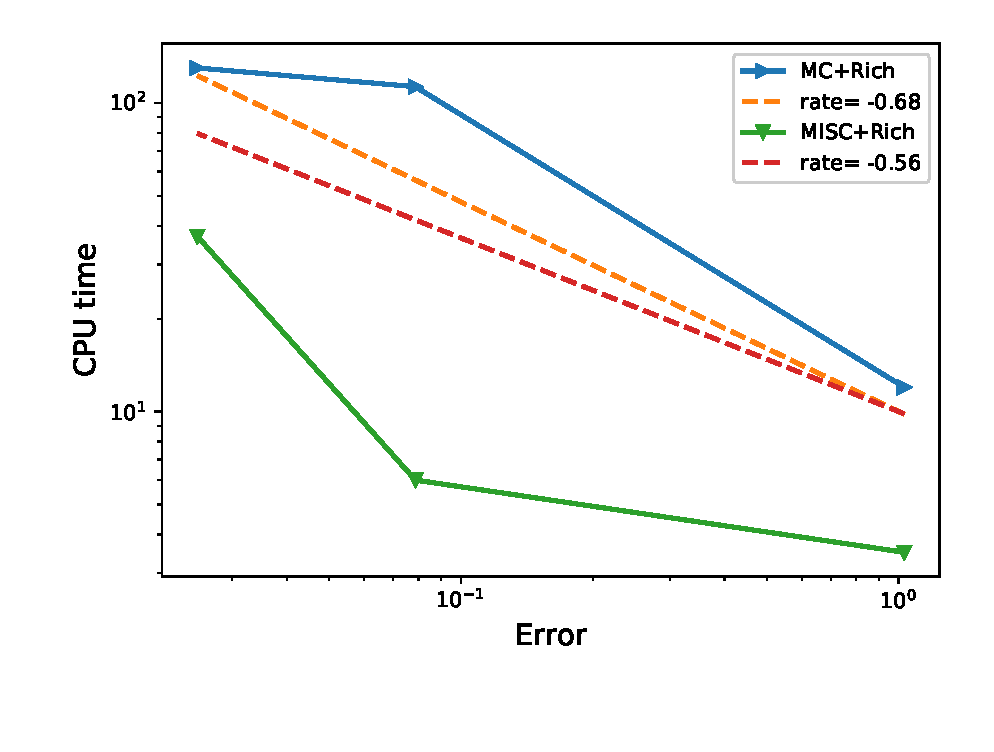
\includegraphics[width=0.7\linewidth]{./figures/rBergomi_Complexity_rates/set2/error_vs_time_set2_rich_linear}

\caption{Complexity plot for  MC and MISC with Richardson extrapolation, for Case set $2$ parameters of table \ref{table:Reference solution, using MC with $500$ time steps, of Call option price under rBergomi model, for different parameter constellation.}.}
\label{fig:Complexity plot for MC and MISC for Case set $2$ parameters, richardson,linear}
\end{figure}


%\begin{figure}[h!]
%\centering
%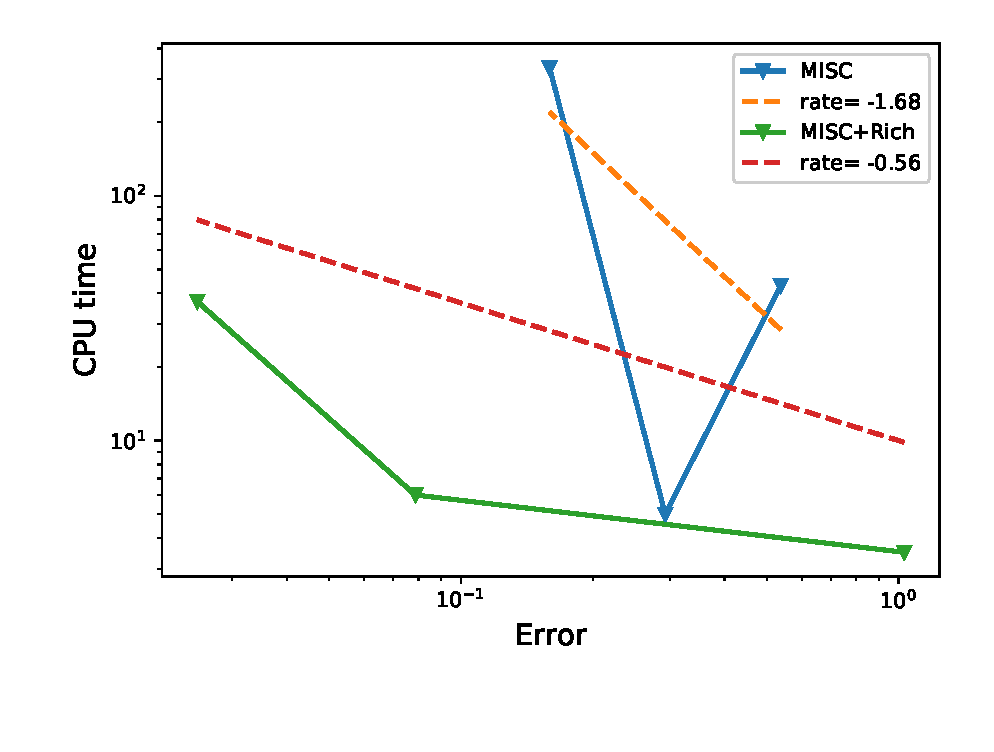
\includegraphics[width=0.7\linewidth]{./figures/rBergomi_Complexity_rates/set2/error_vs_time_set2_comparison_linear}
%
%\caption{Complexity plot for  MISC (with/without) Richardson extrapolation for Case set $2$ parameters of table \ref{table:Reference solution, using MC with $500$ time steps, of Call option price under rBergomi model, for different parameter constellation.}.}
%\label{fig:Complexity plot for  MISC for Case set $2$ parameters, comparison,linear}
%\end{figure}


\FloatBarrier
\subsubsection{Case of set $1$ parameters in table \ref{table:Reference solution, using MC with $500$ time steps, of Call option price under rBergomi model, for different parameter constellation.}}\label{sec:Case of set 1 parameters}


\begin{table}[h!]
	\centering
	\begin{tabular}{l*{6}{c}r}
		Method \textbackslash  Steps            & $2$ & $4$ & $8$ & $16$ &   \\
		\hline
		MISC ($TOl=5.10^{-1}$)  & $0.1140$ & $0.0961$ & $0.0848$ & $0.0781$  \\
		%MISC ($TOl=2.10^{-1}$)  & $0.1140$ & $0.0961$ & $0.0848$ & $\red{0.0769}$  \\
		MISC ($TOl=10^{-1}$)  & $0.1140$ & $0.0961$ & $0.0871$ & $0.0802$  \\
		MISC ($TOl=5.10^{-2}$)  & $0.1140$ & $0.0963$ & $0.0843$ & $0.0824$  \\
		MISC ($TOl=10^{-2}$)  & $0.1077$ & $0.0944$ & $0.0838$ & $0.0772$  \\
		%		MISC ($TOl=5.10^{-3}$)  & $0.1063$ & $0.0931$ & $0.0831$ & $-$  \\
		MISC ($TOl=10^{-3}$)  & $0.1077$ & $0.0921$ & $0.0819$ & $0.0762$  \\
			MISC ($TOl=5.10^{-4}$)  & $0.1079   $ & $0.0921$ & $0.0822$ & $0.0762$  \\
		MISC ($TOl=10^{-4}$)  & $0.1079$ & $0.0921$ & $0.0822$ & $-$  \\
		\hline
		MC method ($M=8.10^{6}$)   & $  0.1078$ & $ 0.0921
		$  & $   0.0822
		$ & $ 0.0767$ \\		
		
		\hline
	\end{tabular}
	\caption{ Call option price of the different methods for different number of time steps. Case of set $1$ parameters in table \ref{table:Reference solution, using MC with $500$ time steps, of Call option price under rBergomi model, for different parameter constellation.}, without Richardson extrapolation.}
	\label{table: Call option price of the different methods for different number of time steps. Case set 1}
\end{table}


\begin{table}[h!]
	\centering
	\begin{tabular}{l*{6}{c}r}
		Method \textbackslash  Steps            & $2$ & $4$ & $8$ & $16$  \\
		\hline
		MC Bias ($M=8.10^6$)   & 	$ \underset{( 0.0366)}{\mathbf{0.5142}}$  & $\underset{( 0.0209)}{\mathbf{0.2933}}$  & $\underset{( 0.0110)}{\mathbf{0.1551}}$ & $\underset{( 0.0055)}{\mathbf{0.0777}}$\\ 
		
		MC Statistical error ($M=8.10^6$)  &  $\underset{(  6.0e-05)} {\mathbf{8.4e-04}}$  & $\underset{(3.4e-05)} {\mathbf{4.8e-04}}$  & $\underset{(2.7e-05)} {\mathbf{ 3.8e-04}}$ & $\underset{( 2.35e-05)} {\mathbf{3.3e-04}}$	\\
%		MC Statistical error ($M=10^5$)  &  $\underset{(  5.4e-04)} {\mathbf{7.5e-03}}$  & $\underset{(3.1e-04)} {\mathbf{4.3e-03}}$  & $\underset{(2.4e-04)} {\mathbf{ 3.4e-03}}$ & $\underset{( 2.1e-04)} {\mathbf{3.0e-03}}$	\\
		
		%		MC Statistical error ($M=10^4$)  &  $\underset{(  1.4e-03)} {\mathbf{1.9e-02}}$  & $\underset{(9.9e-04)} {\mathbf{1.4e-02}}$  & $\underset{(7.8e-04)} {\mathbf{ 1.1e-02}}$ & $\underset{( 6.4e-04)} {\mathbf{9}}$	\\
		\hline
	\end{tabular}
	\caption{Bias and Statistical errors of MC  for computing Call option price  for different number of time steps. Case set 1, without Richardson extrapolation. The numbers between parentheses are the corresponding absolute errors.}
	\label{Bias and Statistical errors of MC ($M=10^6$)  for computing Call option price  for different number of time steps. Case set 1, without Richardson extrapolation. The numbers between parentheses are the corresponding absolute errors.}
\end{table}



\begin{table}[h!]
	\centering
	\begin{tabular}{l*{6}{c}r}
		Method \textbackslash  Steps            & $2$ & $4$ & $8$ & $16$  \\
		\hline
		MISC ($TOl=5.10^{-1}$)  & $\underset{0.0062}{\mathbf{  0.0868}}$ & $\underset{ 0.0040}{\mathbf{0.0563}}$ & $\underset{ 0.0040}{\mathbf{0.0563}}$ & $\underset{0.0014}{\mathbf{0.0197}}$  \\
		MISC ($TOl=10^{-1}$)  & $\underset{0.0062}{\mathbf{  0.0868}}$ & $\underset{ 0.0040}{\mathbf{0.0563}}$& $\underset{0.0049}{\mathbf{0.0681}}$ & $\underset{0.0035
		}{\mathbf{0.0492}}$  \\
		MISC ($TOl=5.10^{-2}$)  &$\underset{0.0062}{\mathbf{  0.0868}}$ & $\underset{0.0042}{\mathbf{0.0591}}$ & $\underset{0.0021}{\mathbf{0.0288
		}}$ & $\underset{0.0057}{\mathbf{0.0800}}$  \\
		MISC ($TOl=10^{-2}$)  & $\underset{ 0.0001
		}{\mathbf{\red{  0.0017}}}$ & $\underset{ 0.0023}{\mathbf{ 0.0324}}$ & $\underset{0.0016
		}{\mathbf{0.0218
		}}$ & $\underset{0.0005}{\mathbf{\red{0.0070}}}$  \\
		MISC ($TOl=10^{-3}$)  & $\underset{ 0.0001
		}{\mathbf{  0.0017}}$ & $\underset{1.0e-05
	}{\mathbf{ \red{1.4e-04
	}}}$ & $\underset{3.5e-04
		}{\mathbf{  0.0049
		}}$ & $\underset{0.0005}{\mathbf{ 0.0070}}$  \\
	MISC ($TOl=5.10^{-4}$)  & $\underset{ 0.0001
	}{\mathbf{  0.0017}}$ & $\underset{1.0e-05
	}{\mathbf{ 1.4e-04
	}}$ & $\underset{1.5e-04
	}{\mathbf{    0.0021
	}}$ & $\underset{-}{\mathbf{-}}$  \\
		MISC ($TOl=10^{-4}$)  & $\underset{ 0.0001
		}{\mathbf{  0.0017}}$ & $\underset{1.0e-05
	}{\mathbf{ 1.4e-04
}}$ & $\underset{(  4.9e-05)
		}{\mathbf{\red{6.9e-04}
		}}$ & $\underset{-}{\mathbf{-}}$  \\
		\hline
	\end{tabular}
	\caption{Quadrature error of MISC to compute Call option price of the different tolerances for different number of time steps. Case  set $1$ parameters in table \ref{table:Reference solution, using MC with $500$ time steps, of Call option price under rBergomi model, for different parameter constellation.}, without Richardson extrapolation. The numbers between parentheses are the corresponding absolute errors.}
	\label{Quadrature error of MISC to compute Call option price of the different tolerances for different number of time steps. Case  set $1$ parameters, without Richardson extrapolation. The numbers between parentheses are the corresponding absolute errors.}
\end{table}




\begin{figure}[h!]
	\centering
	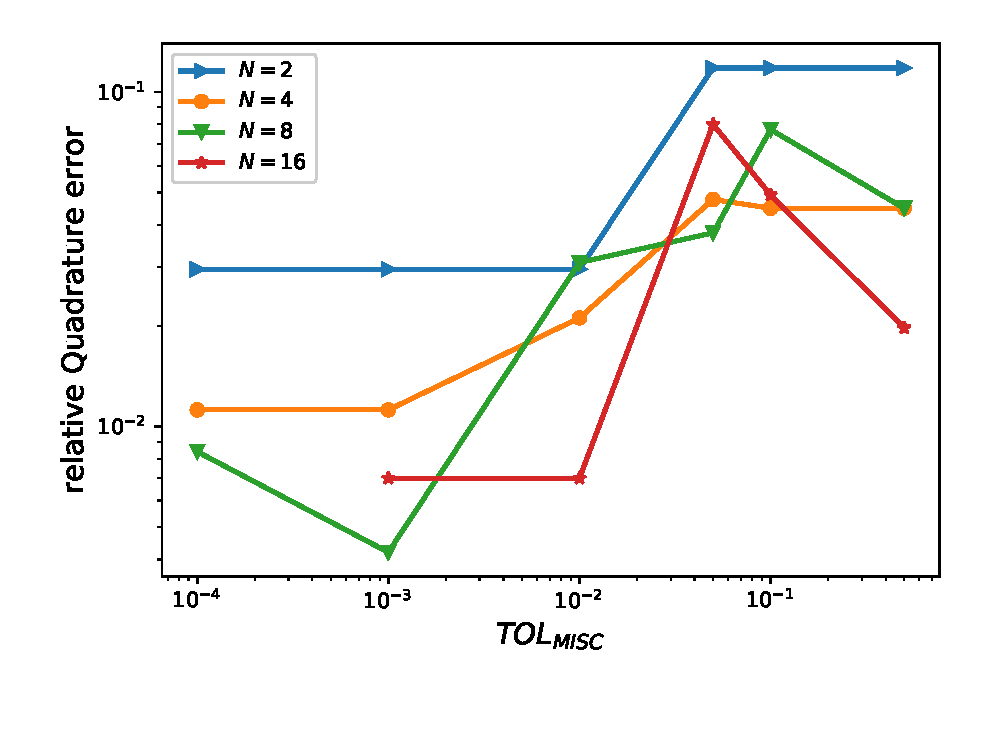
\includegraphics[width=0.7\linewidth]{./figures/rBergomi_MISC_quadratre_error/vs_TOL/set1/relative_quad_error_wrt_MISC_TOL_set1_non_rich}
	
	
	\caption{Quadrature error of MISC to compute Call option price of the different tolerances for different number of time steps. Case  set $1$ parameters, without Richardson extrapolation.}
	\label{fig:Quadrature_error_set1}
\end{figure}




\begin{table}[h!]
	\centering
	\begin{tabular}{l*{6}{c}r}
		Method \textbackslash  Steps            & $2$ & $4$ & $8$ & $16$  \\
		\hline
		MISC ($TOl=5.10^{-1}$)  & $\mathbf{0.6010}$ & $\mathbf{0.3496}$ & $\mathbf{ 0.2114}$ & $\mathbf{ 0.0974}$  \\
		MISC ($TOl=10^{-1}$)  & $\mathbf{0.6010}$ & $\mathbf{0.3496}$ & $\mathbf{  0.2232}$ & $\mathbf{
			0.1269}$  \\
		MISC ($TOl=5.10^{-2}$)  &$\mathbf{0.6010}$ & $\mathbf{  0.3524}$ & $\mathbf{ 0.1839}$ & $\mathbf{  0.1577}$  \\
		MISC ($TOl=10^{-2}$)  & $\mathbf{\red{0.5159}}$ & $\mathbf{0.3257}$ & $\mathbf{ 0.1769}$ & $\mathbf{  \red{0.0847}}$  \\
		MISC ($TOl=10^{-3}$)  & $\mathbf{0.5159}$ & $\mathbf{\red{0.2934}}$ & $\mathbf{0.1600}$ & $\mathbf{0.0847}$  \\
		MISC ($TOl=5.10^{-4}$)  & $\mathbf{0.5159}$ & $\mathbf{0.2934}$ & $\mathbf{0.1572}$ & $\mathbf{-}$  \\
		MISC ($TOl=10^{-4}$)  & $\mathbf{0.5159}$ & $\mathbf{0.2934}$ & $\mathbf{\red{0.1558}}$ & $\mathbf{-}$  \\
		\hline
		MC     & $\mathbf{\red{0.5159}}$ & $\mathbf{\red{0.2938}}$ & $\mathbf{\red{0.1555}}$ &$\mathbf{  \red{0.0817}}$  \\	
%		MC  ($M=10^6$)   & $\mathbf{
%			0.4844}$  & $\mathbf{    0.3056
%		}$  & $\mathbf{0.1477
%		}$ & $\mathbf{0.0786
%		}$  \\	
%		
%		MC  ($M=10^5$)   & $\mathbf{
%			0.4900}$  & $\mathbf{  0.3085 
%		}$  & $\mathbf{0.1500
%		}$ & $\mathbf{0.0807
%		}$  \\			
		
		%	MC  ($M=10^4$)   & $\mathbf{
		%	0.5015}$  & $\mathbf{    0.3182
		%}$  & $\mathbf{0.1576
		%}$ & $\mathbf{0.0867
		%}$  \\
		\hline
	\end{tabular}
	\caption{Total error of MISC and MC to compute Call option price of the different tolerances for different number of time steps. Case Case set $1$ parametrs of table \ref{table:Reference solution, using MC with $500$ time steps, of Call option price under rBergomi model, for different parameter constellation.}, without Richardson extrapolation..}
	\label{Total error of MISC and MC to compute Call option price of the different tolerances for different number of time steps. Case set 1, without Richardson extrapolation. The numbers between parentheses are the corresponding absolute errors.}
\end{table}



\begin{table}[h!]
	\centering
	\begin{tabular}{l*{6}{c}r}
		Method \textbackslash  Steps            & $2$ & $4$ & $8$ & $16$ &   \\
		\hline
		MISC ($TOl=5.10^{-1}$)  & $0.1$ & $0.1$ & $0.2$ & $0.4$  \\
		MISC ($TOl=10^{-1}$)  & $0.1$ & $0.1$ & $0.6$ & $6$  \\
		MISC ($TOl=5.10^{-2}$)  & $0.1$ & $0.3$ & $2$ & $14$  \\
		MISC ($TOl=10^{-2}$)  & $\red{0.2}$ & $1$ & $9$ & $\red{215}$  \\
		MISC ($TOl=10^{-3}$)  & $2$ & $\red{11}$ & $243$ & $4650$  \\
			MISC ($TOl=5.10^{-4}$)  & $3$ & $17$ & $ 670$ & $-$  \\
		MISC ($TOl=10^{-4}$)  & $6$ & $96$ & $\red{5760}$ & $-$  \\
		\hline
			MC     & $\mathbf{\red{ 50}}$  & $\mathbf{\red{344}}$  & $\mathbf{\red{637}}$ & $\mathbf{\red{8}}$  \\
%		MC method ($M=10^6$)   & $29$  & $32$  & $37$ & $51$  \\
%		MC method ($M=10^5$)   & $3$  & $3$  & $4$ & $5$  \\
		%			MC method ($M=10^4$)   & $0.4$  & $0.4$  & $0.5$ & $0.6$  \\	
	\hline
			Ratio of $\left(\text{MC}/ \text{MISC} \right)$  &$\red{  250}$ & $\red{    31
		}$  & $\red{ 0.1
		}$  & $\red{  0.04}$ \\
		\hline
	\end{tabular}
	\caption{Comparsion of the computational time of  MC and MISC, used to compute Call option price of rBergomi model for different number of time steps. Case set $1$ parametrs of table \ref{table:Reference solution, using MC with $500$ time steps, of Call option price under rBergomi model, for different parameter constellation.}. The
average MC CPU time is computed over 10 runs. }
	\label{Comparison of the computational time of  MC and MISC, used to compute Call option price of rBergomi model for different number of time steps. Case set1}
\end{table}

	\begin{figure}[h!]
	\centering
	\includegraphics[width=0.7\linewidth]{./figures/rBergomi_Complexity_rates/set1/error_vs_time_set1}
	
	\caption{Complexity plot for   MC and MISC for Case set $1$ parameters of table \ref{table:Reference solution, using MC with $500$ time steps, of Call option price under rBergomi model, for different parameter constellation.}.}
	\label{fig:Complexity plot for MC and MISC for Case set $1$ parameters}
\end{figure}


%\begin{table}[h!]
%	\centering
%	\begin{tabular}{l*{6}{c}r}
%		Method \textbackslash  Steps            & $2$ & $4$ & $8$ & $16$ &   \\
%		\hline
%		%		MISC ($TOl=5.10^{-1}$)  & $0.6011$ & $0.3497$ & $0.1910$ & $0.0969$  \\
%		MISC ($TOl=2.10^{-1}$)  &  $0.6011$ & $0.3497$ &$0.1910$ & $\red{0.0801}$  \\
%		MISC ($TOl=10^{-1}$)  & $0.6011$ & $0.3497$ & $0.2233$ & $-$  \\
%		%		MISC ($TOl=5.10^{-2}$)  & $0.6011$ & $0.3539$ & $0.1882$ & $0.1573$  \\
%		MISC ($TOl=10^{-2}$)  & $\red{0.5126}$ & $0.3258$ & $0.1770$ & $-$   \\	
%		%		MISC ($TOl=5.10^{-3}$)  & $	0.4930$ & $0.3076$ & $0.1671$ & $-$   \\	
%		MISC ($TOl=10^{-3}$)  & $	-$ & $\red{0.2935}$ & $\red{0.1503}$ & $-$   \\
%		%		MISC ($TOl=10^{-4}$)  & $		0.5154$ & $0.2935$ & $-$ & $-$   \\
%		MC method ($M=10^{6}$)   & $\mathbf{0.5154}$  & $\mathbf{0.2935}$  & $\mathbf{0.1545}$ & $\mathbf{0.0801}$  \\	
%		\hline
%	\end{tabular}
%	\caption{Relative error of Call option price of the different tolerances for different number of time steps. Case $K=1$, $H=0.43$, without Richardson extrapolation}
%	\label{Relative error of Call option price of the different tolerances for different number of time steps. Case $K=1, H=0.43$}
%\end{table}






\begin{table}[h!]
	\centering
	\begin{tabular}{l*{6}{c}r}
		Method \textbackslash  Steps    &$1-2$         & $2-4$ & $4-8$ & $8-16$\\
		\hline
		MISC ($TOl=5.10^{-1}$)& $0.1357$  & $0.0783$ & $0.0735$ & $0.0714$ \\
		MISC ($TOl=10^{-1}$)  &$0.1357$  &$0.0783$ & $0.0785$ & $0.0761$  \\
		MISC ($TOl=5.10^{-2}$)  & $0.1357$ & $0.0831$ & $0.0773$ & $0.0758$   \\
		MISC ($TOl=10^{-2}$)  & $0.1237$ &$0.0781$ & $0.0745$ & $0.0714$  \\
		%		MISC ($TOl=5.10^{-3}$)  & $0.1225$ &$0.0779$ & $0.0727$ & $-$  \\	
		MISC ($TOl=10^{-3}$)  & $0.1224$ &$0.0766$ & $0.0720$ & $0.0705$ \\
		MISC ($TOl=10^{-4}$)  &$0.1224$ & $0.0763$ & $0.0724$ & $-$ \\
		\hline
		MC method ($M=10^6$)  &$	0.1237$ & $0.0752$ & $0.0721$ & $  0.0713$ \\
		\hline
	\end{tabular}
	\caption{Call option price of the different methods for different number of time steps. Case set $1$ parameters of table \ref{table:Reference solution, using MC with $500$ time steps, of Call option price under rBergomi model, for different parameter constellation.}, using Richardson extrapolation (level $1$)}
	\label{table:  Call option price of the different methods for different number of time steps. Case set $1$ parameter, using Richardson extrapolation (level $1$)}
\end{table}




\begin{table}[h!]
	\centering
	\begin{tabular}{l*{6}{c}r}
		Method \textbackslash  Steps            & $1-2$ & $2-4$ & $4-8$ & $8-16$  \\
		\hline
		MC ($M=10^6$)  Bias   &$\underset{( 0.0525)}{\mathbf{0.7378}}$  & $\underset{(    0.0040)}{\mathbf{0.0561}}$  & $\underset{(0.0009 )}{\mathbf{0.0127}}$  & $\underset{(0.0001)}{\mathbf{0.0021}}$ \\	
		
		MC Statistical error ($M=10^6$)   & $\underset{( 2.3e-04)}{\mathbf{3.3e-03}}$  & $\underset{(  1.1e-04)}{\mathbf{1.6e-03}}$  & $\underset{(7.1e-05)}{\mathbf{1.0e-03}}$ & $\underset{(   6.4e-05 )}{\mathbf{9.0e-04}}$ \\	
		%MC Statistical error  ($M=10^4$)  & $\underset{( 1.8e-03)}{\mathbf{2.5e-02}}$  & $\underset{(  8.5e-04)}{\mathbf{1.2e-02}}$  & $\underset{(7.1e-04)}{\mathbf{1.0e-02}}$ & $\underset{(   6.5e-04 )}{\mathbf{9.1e-03}}$ \\
		
%		
%		MC Statistical error  ($M=10^5$)  & $\underset{( 6.7e-04)}{\mathbf{9.5e-03}}$  & $\underset{(  3.8e-04)}{\mathbf{5.3e-03}}$  & $\underset{(2.3e-04)}{\mathbf{3.2e-03}}$ & $\underset{(2.1e-04)}{\mathbf{2.9e-03}}$ \\
		\hline
	\end{tabular}
	\caption{Bias and Statistical errors of MC   for computing Call option price  for different number of time steps. Case set $1$ parameters in tabel \ref{table:Reference solution, using MC with $500$ time steps, of Call option price under rBergomi model, for different parameter constellation.}, with Richardson extrapolation (level $1$). The numbers between parentheses are the corresponding absolute errors.}
	\label{Bias and Statistical errors of MC ($M=10^6$)  for computing Call option price  for different number of time steps. Case set $1$ parameters, with Richardson extrapolation (level1). The numbers between parentheses are the corresponding absolute errors.}
\end{table}



\begin{table}[!h]
	\centering
	\begin{tabular}{l*{6}{c}r}
		Method \textbackslash  Steps            & $1-2$ & $2-4$ & $4-8$ & $8-16$  \\
		\hline
		MISC ($TOl=5.10^{-1}$)  & $\underset{(  0.0120)}{\mathbf{   0.1685}}$ & $\underset{(0.0031)}{\mathbf{0.0435}}$ & $\underset{(0.0014
			)}{\mathbf{ 0.0197}}$ & $\underset{(0.0001)}{\mathbf{0.0014}}$ \\
		MISC ($TOl=10^{-1}$)  & $\underset{(  0.0120)}{\mathbf{   0.1685}}$ & $\underset{(0.0031)}{\mathbf{0.0435}}$ & $\underset{(0.0064)}{\mathbf{0.0899}}$ & $\underset{(0.0048)}{\mathbf{0.0674}}$  \\
		MISC ($TOl=5.10^{-2}$)  & $\underset{(  0.0120)}{\mathbf{   0.1685}}$ & $\underset{(0.0079)}{\mathbf{0.1109}}$ & $\underset{(0.0052)}{\mathbf{0.0730}}$ & $\underset{(0.0045)}{\mathbf{0.0632}}$  \\
		MISC ($TOl=10^{-2}$)  & $\underset{(7e-07)}{\mathbf{1e-05}}$ &    $\underset{(0.0029)}{\mathbf{0.0407}}$ & $\underset{(0.0024  )}{\mathbf{0.0337}}$ & $\underset{(0.0001)}{\mathbf{0.0014}}$  \\
		MISC ($TOl=10^{-3}$)  & $\underset{(0.0013)}{\mathbf{
				\red{0.0183}}}$ &    $\underset{(0.0014
			)}{\mathbf{\red{0.0197}}}$ & $\underset{(0.0001)}{\mathbf{ \red{0.0014}
		}}$ & $\underset{(0.0008)}{\mathbf{0.0112}}$  \\
		
		MISC ($TOl=10^{-4}$)  & $\underset{(0.0013)}{\mathbf{
				0.0183}}$ &    $\underset{(0.0011
			
			)}{\mathbf{0.0154}}$ & $\underset{(0.001)}{\mathbf{   0.0014
		}}$ & $\underset{(-)}{\mathbf{-}}$  \\
		\hline
	\end{tabular}
	\caption{Quadrature error of MISC to compute Call option price of the different tolerances for different number of time steps. Case set $1$ parameters in table \ref{table:Reference solution, using MC with $500$ time steps, of Call option price under rBergomi model, for different parameter constellation.}, with Richardson extrapolation(level $1$). The numbers between parentheses are the corresponding absolute errors.}
	\label{Quadrature error of MISC to compute Call option price of the different tolerances for different number of time steps. Case set $1$ parameters, with Richardson extrapolation(level $1$). The numbers between parentheses are the corresponding absolute errors.}
\end{table}





\begin{figure}[h!]
	\centering
	\includegraphics[width=0.7\linewidth]{./figures/rBergomi_MISC_quadratre_error/vs_TOL/set1/relative_quad_error_wrt_MISC_TOL_set1_with_rich}
	
	
	\caption{Quadrature error of MISC to compute Call option price of the different tolerances for different number of time steps. Case  set $1$ parameters, with Richardson extrapolation.}
	\label{fig:Quadrature_error_set1_rich}
\end{figure}



\begin{table}[!h]
	\centering
	\begin{tabular}{l*{6}{c}r}
		Method \textbackslash  Steps            & $1-2$ & $2-4$ & $4-8$ & $8-16$  \\
		\hline
		MISC ($TOl=5.10^{-1}$)  & $\mathbf{0.9063
		}$ & $\mathbf{ 0.0996}$ & $\mathbf{0.0324
		}$ & $\mathbf{ 0.0035}$ \\
		MISC ($TOl=10^{-1}$)  & $\mathbf{0.9063
		}$ & $\mathbf{ 0.0996}$ & $\mathbf{  0.1026}$ & $\mathbf{ 0.0695
		}$  \\
		MISC ($TOl=5.10^{-2}$)  & $\mathbf{0.9063
		}$ & $\mathbf{    0.1670}$ & $\mathbf{ 0.0857}$ & $\mathbf{0.0653
		}$  \\
		MISC ($TOl=10^{-2}$)  & $\mathbf{0.7378}$ & $\mathbf{  0.0968}$ & $\mathbf{   0.0464}$ & $\mathbf{ 0.0035}$  \\	
		MISC ($TOl=10^{-3}$)  & $\mathbf{\red{0.7561}}$ & $\mathbf{\red{0.0758}}$ & $\mathbf{\red{0.0141}}$ & $\mathbf{-}$  \\
		MISC ($TOl=10^{-4}$)  & $\mathbf{0.7561}$ & $\mathbf{0.0715}$ & $\mathbf{0.0141}$ & $\mathbf{-}$  \\
		\hline
			MC   & $\mathbf{\red{0.7561}}$  & $\mathbf{\red{0.0758}}$  & $\mathbf{\red{0.0141}}$ &$\mathbf{-}$   \\
%		MC ($M=10^6$)  & $\mathbf{0.7411}$  & $\mathbf{ 0.0577}$  & $\mathbf{  0.0137}$ &$\mathbf{  0.0030}$   \\	
%		%MC ($M=10^4$)  & $\mathbf{0.7628}$  & $\mathbf{ 0.0681}$  & $\mathbf{  0.0227}$ &$\mathbf{  0.0112}$   \\
%		MC ($M=10^5$)  & $\mathbf{0.7473}$  & $\mathbf{ 0.0614}$  & $\mathbf{  0.0159}$ &$\mathbf{  0.0050}$   \\
		\hline
	\end{tabular}
	\caption{Total  error of MISC and MC to compute Call option price of the different tolerances for different number of time steps. Case set $1$ parameters in table \ref{table:Reference solution, using MC with $500$ time steps, of Call option price under rBergomi model, for different parameter constellation.}, with Richardson extrapolation(level $1$).}
	\label{Total  error of MISC and MC to compute Call option price of the different tolerances for different number of time steps. Case set $1$ parameters, with Richardson extrapolation(level $1$). The numbers between parentheses are the corresponding absolute errors.}
\end{table}

\begin{table}[!h]
	\centering
	\begin{tabular}{l*{6}{c}r}
		Method \textbackslash  Steps            & $1-2$ & $2-4$ & $4-8$ & $8-16$ &   \\
		\hline
		MISC ($TOl=5.10^{-1}$)  & $0.1$ & $0.1$ & $0.2$ & $0.5$  \\
		MISC ($TOl=10^{-1}$)  & $0.1$ & $0.1$ & $0.6$ & $8$  \\
		MISC ($TOl=5.10^{-2}$)  & $0.1$ & $0.4$ & $2$ & $38$  \\
		MISC ($TOl=10^{-2}$)  & $1$ & $2$ & $18$ & $490$  \\
		MISC ($TOl=10^{-3}$)  & $\red{4}$ & $\red{12}$ & $\red{520}$ & $54065$  \\	
		MISC ($TOl=10^{-4}$)  & $7$ & $191$ & $7650$ & $-$  \\
		\hline
			MC   & $\mathbf{\red{ 34.7}}$  & $\mathbf{\red{37}}$  & $\mathbf{ \red{532}}$ &$\mathbf{-}$   \\
%		MC method + Richardson (level 1) ($M=10^{6}$)  &$43$ & $46$  & $53$  & $72$ \\	
%		%MC method + Richardson (level 1) ($M=10^{4}$)  &$0.6$ & $0.6$  & $0.7$  & $0.8$ \\	
%		MC method + Richardson (level 1) ($M=10^{5}$)  &$5$ & $5$  & $6$  & $8$ \\	
		\hline
			Ratio of $\left(\text{MC}/ \text{MISC} \right)$  &$\red{8.7}$ & $\red{   3.1
		}$  & $\red{1}$ &  $-$ \\
		\hline
	\end{tabular}
	\caption{Comparsion of the computational time of  MC and MISC, using Richardson extrapolation (level $1$), used to compute Call option price of rBergomi model for different number of time steps. Case set $1$ parameters in table \ref{table:Reference solution, using MC with $500$ time steps, of Call option price under rBergomi model, for different parameter constellation.}. The
average MC CPU time is computed over 10 runs.}
	\label{Comparsion of the computational time of  MC and MISC, using Richardson extrapolation (level $1$), used to compute Call option price of rBergomi model for different number of time steps. Case set $1$ parameters}
\end{table}





\begin{figure}[h!]
	\centering
	\includegraphics[width=0.7\linewidth]{./figures/rBergomi_Complexity_rates/set1/error_vs_time_set1_rich}
	
	\caption{Complexity plot for  MC and MISC with Richardson extrapolation, for Case set $1$ parameters of table \ref{table:Reference solution, using MC with $500$ time steps, of Call option price under rBergomi model, for different parameter constellation.}.}
	\label{fig:Complexity plot for MC and MISC for Case set $1$ parameters, richardson}
\end{figure}


\begin{figure}[h!]
	\centering
	\includegraphics[width=0.7\linewidth]{./figures/rBergomi_Complexity_rates/set1/error_vs_time_set1_comparison}
	
	\caption{Complexity plot for  MISC (with/without) Richardson extrapolation for Case set $1$ parameters of table \ref{table:Reference solution, using MC with $500$ time steps, of Call option price under rBergomi model, for different parameter constellation.}.}
	\label{fig:Complexity plot for  MISC for Case set $1$ parameters, comparison}
\end{figure}

\FloatBarrier


%\begin{table}[h!]
%	\centering
%	\begin{tabular}{l*{5}{c}r}
%		Method \textbackslash  Steps    &$1-2$        & $2-4$ & $4-8$ & $8-16$  \\
%		\hline
%		MISC ($TOl=5.10^{-1}$)  &$0.9059$ & $0.0997$ & $0.0323$ & $\red{0.0028}$  \\
%		MISC ($TOl=10^{-1}$)  &$0.9059$ &$0.0997$ & $0.1025$ & $-$ \\
%		%		MISC ($TOl=5.10^{-2}$)  &$0.9059$ & $0.1671$ & $0.0857$ & $0.0646$   \\
%		MISC ($TOl=10^{-2}$)  & $0.7374$ &$0.0969$ & $0.0463$ & $-$ \\		
%		%		MISC ($TOl=5.10^{-3}$)  & $0.7205$ &$0.0941$ & $0.0211$ & $-$ \\	
%		MISC ($TOl=10^{-3}$)  & $0.7191$ & $0.0758$ & $\red{0.0112}$ & $-$ \\	
%		MISC ($TOl=5.10^{-4}$)  &$\red{0.7129}$ & $\red{0.0609}$ & $-$ & $-$ \\
%		MC method ($M=10^{6}$)&$ \mathbf{0.7133}$    & $\mathbf{0.0698}$  & $\mathbf{0.0160}$  & $\mathbf{0.0035}$ \\
%		\hline
%	\end{tabular}
%	\caption{Relative error of Call option price of the different tolerances for different number of time steps. Case $K=1$, $H=0.43$, using Richardson extrapolation (level $1$)}
%	\label{Relative error of Call option price of the different tolerances for different number of time steps. Case $K=1, H=0.43$ , using Richardson extrapolation}
%\end{table}



%\begin{table}[h!]
%	\centering
%	\begin{tabular}{l*{5}{c}r}
%		Method \textbackslash  Steps    &$1-2-4$        & $2-4-8$ & $4-8-16$   \\
%		\hline
%		MISC ($TOl=5.10^{-1}$)  &$ 0.1699$ & $\red{0.0098}$ & $ 0.0056$   \\
%		MISC ($TOl=2.10^{-1}$)  &$ 0.1699$ &$-$ & $\red{ 0.0014}$  \\
%		MISC ($TOl=10^{-1}$)  &$0.2037$ &$-$ & $-$  \\
%		MISC ($TOl=5.10^{-2}$)  &$\red{0.0295}$ & $-$ & $-$  \\
%		MC method ($M=10^{6}$)&$\mathbf{0.1440}$    & $ \mathbf{0.0180}  $  & $\mathbf{0.0023}$   \\
%		\hline
%	\end{tabular}
%	\caption{Relative error of Call option price of the different tolerances for different number of time steps. Case $K=1$, $H=0.43$, using Richardson extrapolation (level $2$)}
%	\label{Relative error of Call option price of the different tolerances for different number of time steps. Case $K=1, H=0.43$ , using Richardson extrapolation_level2}
%\end{table}
%
%
%
%
%
%
%
%
%
%
%
%\begin{table}[h!]
%	\centering
%	\begin{tabular}{l*{6}{c}r}
%		Method \textbackslash  Steps           &$1-2-4$ & $2-4-8$ & $4-8-16$\\
%		\hline
%		MISC ($TOl=5.10^{-1}$)& $0.0591$  & $\red{0.0719}$ & $0.0708$  \\
%		MISC ($TOl=2.10^{-1}$)  &$0.0591$ &$-$ & $\red{0.0711}$  \\
%		MISC ($TOl=10^{-1}$)  &$0.0567$  &$-$ & $-$   \\
%		MISC ($TOl=5.10^{-2}$)  & $\red{0.0733}$ & $-$ & $-$  \\
%		\hline
%	\end{tabular}
%	\caption{ Call option price of the different methods for different number of time steps. Case $K=1$, $H=0.43$, using Richardson extrapolation (level 2)}
%	\label{table: Call option price of the different methods for different number of time steps. Case $K=1$, using Richardson extrapolation_level2}
%\end{table}


%\newpage
%\subsection{Case of set $2$ parameters in table  \ref{table:Reference solution, using MC with $500$ time steps, of Call option price under rBergomi model, for different parameter constellation.}}\label{appendix:Case of set 2 parameters}
%
%
%
%
%\begin{table}[h!]
%	\centering
%	\begin{tabular}{l*{6}{c}r}
%		Method \textbackslash  Steps    &$1-2-4$         & $2-4-8$ & $4-8-16$ \\
%		\hline
%%		MISC ($TOl=5.10^{-1}$)  &$0.0589$ & $0.0658$ & $0.0659$  \\
%		MISC ($TOl=10^{-1}$)  &$0.0589$ & $0.0668$ & $\red{0.079}$   \\
%		MISC ($TOl=7.10^{-2}$)   &$0.0554$ & $\red{0.0810}$ & $-$   \\
%		MISC ($TOl=5.10^{-2}$)   &$0.0406$ & $-$ & $-$   \\
%		MISC ($TOl=10^{-2}$)  &$\red{0.0654}$ & $-$ & $-$   \\	
%		\hline
%	\end{tabular}
%	\caption{ Call option price of the different methods for different number of time steps. Case $K=1$, $H=0.07$, using Richardson extrapolation (level $2$)}
%	\label{table: Call option price of the different methods for different number of time steps. Case $K=1$, $H=0.07$, using Richardson extrapolation_level2}
%\end{table}
%
%
%\begin{table}[h!]
%	\centering
%	\begin{tabular}{l*{5}{c}r}
%		Method \textbackslash  Steps &$1-2-4$             & $2-4-8$ & $4-8-16$   \\
%		\hline
%		%		MISC ($TOl=5.10^{-1}$)  &$0.2563$ & $ 0.1692$ & $ 0.1679
%		%		$   \\
%		MISC ($TOl=10^{-1}$)  &$0.2563$ &  $0.1566$ & $\red{  0.0025}$  \\
%		MISC ($TOl=7.10^{-2}$) &$  0.3005$ &  $  \red{0.0227}$ & $-$    \\
%		MISC ($TOl=5.10^{-2}$) &$0.4874$ &  $  -$ & $-$    \\
%		MISC ($TOl=10^{-2}$)&$ \red{0.1742}$ &  $-$ & $-$  \\	
%		MC method ($M=10^{6}$)  &$\mathbf{0.2231}$  & $  \mathbf{0.0279}$  & $\mathbf{0.0035}$ \\
%		\hline	
%		
%	\end{tabular}
%	\caption{Relative error of Call option price of the different tolerances for different number of time steps. Case $K=1$, $H=0.07$, using Richardson extrapolation (level $2$)}
%	\label{Relative error of Call option price of the different tolerances for different number of time steps. Case $K=1, H=0.07$ , using Richardson extrapolation_level2}
%\end{table}
%
%
%
%\begin{table}[h!]
%	\centering
%	\begin{tabular}{l*{5}{c}r}
%		Method \textbackslash  Steps &$1-2-4$             & $2-4-8$ & $4-8-16$   \\
%		\hline
%		MISC +Richardson (level 2) &$19$ & $ 33$ & $-$   \\
%		
%		MC method+Richardson (level 2) ($M=10^{6}$)  &$66$  & $74 $  & $95$ \\
%		\hline	
%		
%	\end{tabular}
%	\caption{Comparsion of the computational time of  MC and MISC, coupled with Richardson extrapolation (level $2$), used to compute Call option price of rBergomi model for different number of time steps. Case $K=1, H=0.07$}
%	\label{Comparsion of the computational time of  MC and MISC, coupled with Richardson extrapolation (level $2$), used to compute Call option price of rBergomi model for different number of time steps. Case $K=1, H=0.07$}
%\end{table}

%\subsubsection{Case of set $1$ parameters in table \ref{table:Reference solution, using MC with $500$ time steps, of Call option price under rBergomi model, for different parameter constellation.} with linear hierarchy}
%\label{sec:Case of set $1$ parameters_linear}
%
%\begin{table}[h!]
%\centering
%\begin{tabular}{l*{6}{c}r}
%Method \textbackslash  Steps            & $2$ & $4$ & $8$ & $16$ &   \\
%\hline
%MISC ($TOl=5.10^{-1}$)  & $0.1156$ & $0.0973$ & $0.0857$ & $0.0790$  \\
%
%MISC ($TOl=10^{-1}$)  & $0.1156$ & $0.0973$ & $0.0884$ & $0.0786$  \\
%MISC ($TOl=5.10^{-2}$)  & $0.1156$ & $0.0963$ & $0.0843$ & $0.0815$  \\
%MISC ($TOl=10^{-2}$)  & $0.1082$ & $0.0940$ & $0.0834$ & $0.0764$  \\
%
%MISC ($TOl=10^{-3}$)  & $0.1079$ & $0.0921$ & $0.0820$ & $0.0764$  \\
%MISC ($TOl=10^{-4}$)  & $0.1078$ & $0.0921$ & $0.0820$ & $-$  \\
%\hline
%MC method ($M=8.10^{6}$)   & $  0.1078$ & $ 0.0921
%$  & $   0.0822
%$ & $ 0.0767$ \\		
%
%\hline
%\end{tabular}
%\caption{ Call option price of the different methods for different number of time steps. Case of set $1$ parameters in table \ref{table:Reference solution, using MC with $500$ time steps, of Call option price under rBergomi model, for different parameter constellation.}, without Richardson extrapolation.}
%\label{table: Call option price of the different methods for different number of time steps. Case set 1,linear}
%\end{table}
%
%
%
%
%
%
%\begin{table}[h!]
%\centering
%\begin{tabular}{l*{6}{c}r}
%Method \textbackslash  Steps            & $2$ & $4$ & $8$ & $16$  \\
%\hline
%MISC ($TOl=5.10^{-1}$)  & $\underset{  0.0078}{\mathbf{  0.1095
%}}$ & $\underset{0.0052
%
%}{\mathbf{  0.0731
%}}$ & $\underset{0.0035
%}{\mathbf{0.0485}}$ & $\underset{0.0023
%}{\mathbf{0.0323}}$  \\
%MISC ($TOl=10^{-1}$)  & $\underset{  0.0078}{\mathbf{  0.1095
%}}$  & $\underset{0.0052
%
%}{\mathbf{  0.0731
%}}$ & $\underset{0.0062
%}{\mathbf{0.0863}}$ & $\underset{0.0019
%}{\mathbf{0.0267}}$  \\
%MISC ($TOl=5.10^{-2}$)  &$\underset{  0.0078}{\mathbf{  0.1095
%}}$  & $\underset{ 0.0042}{\mathbf{0.0591}}$ & $\underset{0.0021}{\mathbf{0.0288
%}}$ & $\underset{0.0048
%}{\mathbf{0.0674}}$  \\
%MISC ($TOl=10^{-2}$)  & $\underset{    0.0004
%}{\mathbf{     0.0056}}$ & $\underset{ 0.0019
%}{\mathbf{  0.0268
%}}$ & $\underset{0.0012
%}{\mathbf{0.0162}}$ & $\underset{0.0003}{\mathbf{    \red{0.0042}}}$  \\
%MISC ($TOl=10^{-3}$)  & $\underset{ 8.0e-05
%}{\mathbf{\red{0.0011}
%}}$ & $\underset{1.0e-05}{\mathbf{   \red{ 1.4e-04}}}$ & $\underset{     2.5e-04
%}{\mathbf{\red{ 0.0035}
%}}$ &  $\underset{0.0003}{\mathbf{    0.0042}}$ \\
%MISC ($TOl=10^{-4}$)  & $\underset{ 2.0e-05
%}{\mathbf{2.8e-04}}$ & $\underset{1.0e-05}{\mathbf{    1.4e-04}}$ &$\underset{     2.5e-04
%}{\mathbf{0.0035
%}}$ & $\underset{-}{\mathbf{-}}$  \\
%\hline
%\end{tabular}
%\caption{Quadrature error of MISC to compute Call option price of the different tolerances for different number of time steps. Case  set $1$ parameters in table \ref{table:Reference solution, using MC with $500$ time steps, of Call option price under rBergomi model, for different parameter constellation.}, without Richardson extrapolation. The numbers between parentheses are the corresponding absolute errors.}
%\label{Quadrature error of MISC to compute Call option price of the different tolerances for different number of time steps. Case  set $1$ parameters, without Richardson extrapolation. The numbers between parentheses are the corresponding absolute errors,linear}
%\end{table}
%
%
%
%
%\begin{figure}[h!]
%\centering
%\includegraphics[width=0.7\linewidth]{./figures/rBergomi_MISC_quadratre_error/vs_TOL/set1/relative_quad_error_wrt_MISC_TOL_set1_non_rich_linear}
%
%
%\caption{Quadrature error of MISC to compute Call option price of the different tolerances for different number of time steps. Case  set $1$ parameters, without Richardson extrapolation.}
%\label{fig:Quadrature_error_set1_linear}
%\end{figure}
%
%\FloatBarrier
%\begin{table}[h!]
%\centering
%\begin{tabular}{l*{6}{c}r}
%Method \textbackslash  Steps            & $2$ & $4$ & $8$ & $16$  \\
%\hline
%MISC ($TOl=5.10^{-1}$)  & $\mathbf{  0.6237}$ & $\mathbf{  0.3664}$ & $\mathbf{  0.2036}$ & $\mathbf{0.1100 }$  \\
%MISC ($TOl=10^{-1}$)  & $\mathbf{  0.6237}$ & $\mathbf{  0.3664}$ & $\mathbf{    0.2414}$ & $\mathbf{
%	  0.1044}$  \\
%MISC ($TOl=5.10^{-2}$)  &$\mathbf{  0.6237}$ & $\mathbf{    0.3524}$ & $\mathbf{    0.1839}$ & $\mathbf{     0.1451}$  \\
%MISC ($TOl=10^{-2}$)  & $\mathbf{ 0.5198}$ & $\mathbf{0.3201}$ & $\mathbf{  0.1713}$ & $\mathbf{  \red{  0.0819}}$  \\
%MISC ($TOl=10^{-3}$)  & $\mathbf{\red{ 0.5153}}$ & $\mathbf{\red{  0.2934}}$ & $\mathbf{\red{0.1586}}$ & $\mathbf{  0.0819}$  \\
%MISC ($TOl=10^{-4}$)  & $\mathbf{0.5144}$ & $\mathbf{  0.2934}$ & $\mathbf{0.1586}$ & $\mathbf{-}$  \\
%\hline
%MC     & $\mathbf{\red{0.5159}}$ & $\mathbf{\red{  0.2938}}$ & $\mathbf{\red{0.1584}}$ &$\mathbf{  \red{0.0817}}$  \\	
%
%\hline
%\end{tabular}
%\caption{Total error of MISC and MC to compute Call option price of the different tolerances for different number of time steps. Case Case set $1$ parametrs of table \ref{table:Reference solution, using MC with $500$ time steps, of Call option price under rBergomi model, for different parameter constellation.}, without Richardson extrapolation..}
%\label{Total error of MISC and MC to compute Call option price of the different tolerances for different number of time steps. Case set 1, without Richardson extrapolation. The numbers between parentheses are the corresponding absolute errors,linear}
%\end{table}
%
%
%
%
%
%\begin{table}[h!]
%\centering
%\begin{tabular}{l*{6}{c}r}
%Method \textbackslash  Steps            & $2$ & $4$ & $8$ & $16$ &   \\
%\hline
%MISC ($TOl=5.10^{-1}$)  & $0.1$ & $0.1$ & $0.2$ & $0.5$  \\
%MISC ($TOl=10^{-1}$)  & $0.1$ & $0.1$ & $0.7$ & $8$  \\
%MISC ($TOl=5.10^{-2}$)  & $0.1$ & $0.25$ & $2$ & $17$  \\
%MISC ($TOl=10^{-2}$)  & $0.2$ & $1$ & $9$ & $\red{299}$  \\
%MISC ($TOl=10^{-3}$)  & $\red{0.8}$ & $\red{6}$ & $\red{153}$ & $8140$  \\
%MISC ($TOl=10^{-4}$)  & $2$ & $115$ & $4560$ & $-$  \\
%\hline
%MC     & $\mathbf{\red{50}}$  & $\mathbf{\red{344}}$  & $\mathbf{\red{8}}$ & $\mathbf{\red{8}}$  \\
%
%\hline
%Ratio of $\left(\text{MC}/ \text{MISC} \right)$  &$\red{
%63
%}$ & $\red{   57
%}$  & $\red{  0.05
%}$  & $\red{  0.03}$ \\
%\hline
%\end{tabular}
%\caption{Comparsion of the computational time of  MC and MISC, used to compute Call option price of rBergomi model for different number of time steps. Case set $1$ parametrs of table \ref{table:Reference solution, using MC with $500$ time steps, of Call option price under rBergomi model, for different parameter constellation.} }
%\label{Comparison of the computational time of  MC and MISC, used to compute Call option price of rBergomi model for different number of time steps. Case set1,linear}
%\end{table}
%
%
%
%
%
%
%
%
%
%
%
%
%\begin{table}[h!]
%\centering
%\begin{tabular}{l*{6}{c}r}
%Method \textbackslash  Steps    &$1-2$         & $2-4$ & $4-8$ & $8-16$\\
%\hline
%MISC ($TOl=5.10^{-1}$)& $0.1378$  & $0.0789$ & $0.0742$ & $0.0722$ \\
%MISC ($TOl=10^{-1}$)  &$0.1378$  &$0.0789$ & $0.0768$ & $0.0745$  \\
%MISC ($TOl=5.10^{-2}$)  & $0.1378$ & $0.0834$ & $0.0758$ & $0.0762$   \\
%MISC ($TOl=10^{-2}$)  & $0.1230$ &$0.0798$ & $0.0737$ & $0.0706$  \\
%
%MISC ($TOl=10^{-3}$)  & $0.1222$ &$0.0766$ & $0.0724$ & $0.0706$ \\
%MISC ($TOl=10^{-4}$)  &$0.1222$ & $0.0763$ & $0.0724$ & $-$ \\
%\hline
%MC method ($M=10^6$)  &$	0.1237$ & $0.0752$ & $0.0721$ & $  0.0713$ \\
%\hline
%\end{tabular}
%\caption{Call option price of the different methods for different number of time steps. Case set $1$ parameters of table \ref{table:Reference solution, using MC with $500$ time steps, of Call option price under rBergomi model, for different parameter constellation.}, using Richardson extrapolation (level $1$)}
%\label{table:  Call option price of the different methods for different number of time steps. Case set $1$ parameter, using Richardson extrapolation (level $1$),linear}
%\end{table}
%
%
%
%\begin{table}[!h]
%\centering
%\begin{tabular}{l*{6}{c}r}
%Method \textbackslash  Steps            & $1-2$ & $2-4$ & $4-8$ & $8-16$  \\
%\hline
%MISC ($TOl=5.10^{-1}$)  & $\underset{( 0.0141)}{\mathbf{   0.1980}}$ & $\underset{(0.0037)}{\mathbf{0.0520}}$ & $\underset{(0.0021
%		)}{\mathbf{ 0.0295}}$ & $\underset{(0.0009)}{\mathbf{0.0126}}$ \\
%MISC ($TOl=10^{-1}$)  & $\underset{( 0.0141)}{\mathbf{   0.1980}}$ &$\underset{(0.0037)}{\mathbf{0.0520}}$ & $\underset{(0.0047)}{\mathbf{0.0660}}$ & $\underset{(0.0032)}{\mathbf{0.0449}}$  \\
%MISC ($TOl=5.10^{-2}$)  & $\underset{( 0.0141)}{\mathbf{   0.1980}}$ & $\underset{(0.0082)}{\mathbf{0.1152}}$ & $\underset{(0.0037)}{\mathbf{0.0520
%}}$ & $\underset{(0.0049)}{\mathbf{0.0688}}$  \\
%MISC ($TOl=10^{-2}$)  & $\underset{(7e-04)}{\mathbf{  0.0098
%}}$ &    $\underset{(0.0046
%)}{\mathbf{0.0646}}$ & $\underset{(0.0016  )}{\mathbf{0.0225}}$ & $\underset{(0.0007)}{\mathbf{  \red{0.0098}
%}}$  \\
%MISC ($TOl=10^{-3}$)  & $\underset{(
%	0.0015
%	)}{\mathbf{
%		\red{    0.0211
%	}}}$ &    $\underset{(0.0014
%	)}{\mathbf{\red{0.0197}}}$ & $\underset{(0.001)}{\mathbf{   \red{0.0014}
%}}$ &  $\underset{(0.0007)}{\mathbf{  0.0098
%}}$ \\
%
%MISC ($TOl=10^{-4}$)  & $\underset{(
%	0.0015
%	)}{\mathbf{
%	  0.0211
%}}$ &    $\underset{(0.0011
%	
%	)}{\mathbf{0.0154}}$ & $\underset{(0.001)}{\mathbf{   0.0014
%}}$ & $\underset{(-)}{\mathbf{-}}$  \\
%\hline
%\end{tabular}
%\caption{Quadrature error of MISC to compute Call option price of the different tolerances for different number of time steps. Case set $1$ parameters in table \ref{table:Reference solution, using MC with $500$ time steps, of Call option price under rBergomi model, for different parameter constellation.}, with Richardson extrapolation(level $1$). The numbers between parentheses are the corresponding absolute errors.}
%\label{Quadrature error of MISC to compute Call option price of the different tolerances for different number of time steps. Case set $1$ parameters, with Richardson extrapolation(level $1$). The numbers between parentheses are the corresponding absolute errors,linear}
%\end{table}
%
%
%
%
%
%
%
%\begin{table}[!h]
%\centering
%\begin{tabular}{l*{6}{c}r}
%Method \textbackslash  Steps            & $1-2$ & $2-4$ & $4-8$ & $8-16$  \\
%\hline
%MISC ($TOl=5.10^{-1}$)  & $\mathbf{   0.9358
%}$ & $\mathbf{  0.1081}$ & $\mathbf{0.0324
%}$ & $\mathbf{ 0.0035}$ \\
%MISC ($TOl=10^{-1}$)  & $\mathbf{   0.9358
%}$  & $\mathbf{  0.1081}$ & $\mathbf{  0.1026}$ & $\mathbf{ 0.0695
%}$  \\
%MISC ($TOl=5.10^{-2}$)  & $\mathbf{   0.9358
%}$ & $\mathbf{    0.1713}$ & $\mathbf{ 0.0857}$ & $\mathbf{0.0653
%}$  \\
%MISC ($TOl=10^{-2}$)  & $\mathbf{   0.7476
%}$  & $\mathbf{   0.1207}$ & $\mathbf{ 0.0035}$  \\	
%MISC ($TOl=10^{-3}$)  & $\mathbf{\red{  0.7589}}$ & $\mathbf{0.0758}$ & $\mathbf{\red{0.0141}}$ & $\mathbf{-}$  \\
%MISC ($TOl=10^{-4}$)  & $\mathbf{  0.7589}$ & $\mathbf{\red{0.0715}}$ & $\mathbf{0.0141}$ & $\mathbf{-}$  \\
%\hline
%MC   & $\mathbf{\red{0.7561}}$  & $\mathbf{\red{0.0715}}$  & $\mathbf{\red{0.0141}}$ &$\mathbf{-}$   \\
%
%\hline
%\end{tabular}
%\caption{Total  error of MISC and MC to compute Call option price of the different tolerances for different number of time steps. Case set $1$ parameters in table \ref{table:Reference solution, using MC with $500$ time steps, of Call option price under rBergomi model, for different parameter constellation.}, with Richardson extrapolation(level $1$).}
%\label{Total  error of MISC and MC to compute Call option price of the different tolerances for different number of time steps. Case set $1$ parameters, with Richardson extrapolation(level $1$). The numbers between parentheses are the corresponding absolute errors,linear}
%\end{table}
%
%
%
%
%
%
%\begin{table}[!h]
%\centering
%\begin{tabular}{l*{6}{c}r}
%Method \textbackslash  Steps            & $1-2$ & $2-4$ & $4-8$ & $8-16$ &   \\
%\hline
%MISC ($TOl=5.10^{-1}$)  & $0.1$ & $0.1$ & $0.3$ & $0.7$  \\
%MISC ($TOl=10^{-1}$)  & $0.1$ & $0.1$ & $0.6$ & $12$  \\
%MISC ($TOl=5.10^{-2}$)  & $0.1$ & $0.5$ & $3$ & $54$  \\
%MISC ($TOl=10^{-2}$)  & $0.2$ & $1$ & $16$ & $\red{592}$  \\
%MISC ($TOl=10^{-3}$)  & $\red{1}$ & $\red{6}$ & $\red{520}$ & $10220$  \\	
%MISC ($TOl=10^{-4}$)  & $11$ & $160$ & $7250$ & $-$  \\
%\hline
%MC   & $\mathbf{\red{ 34.7}}$  & $\mathbf{\red{37}}$  & $\mathbf{ \red{532}}$ &$\mathbf{-}$   \\
%
%\hline
%Ratio of $\left(\text{MC}/ \text{MISC} \right)$  &$\red{8.7}$ & $\red{   0.2
%}$  & $\red{ 0.8
%}$  & $\red{-}$ \\
%\hline
%\end{tabular}
%\caption{Comparsion of the computational time of  MC and MISC, using Richardson extrapolation (level $1$), used to compute Call option price of rBergomi model for different number of time steps. Case set $1$ parameters in table \ref{table:Reference solution, using MC with $500$ time steps, of Call option price under rBergomi model, for different parameter constellation.}}
%\label{Comparsion of the computational time of  MC and MISC, using Richardson extrapolation (level $1$), used to compute Call option price of rBergomi model for different number of time steps. Case set $1$ parameters,linear}
%\end{table}
%
%
%\FloatBarrier



\subsection{First and mixed differences rates (Geometric hierarchy)}\label{sec:First and mixed differences rates}


In this section, we plot the first and second order differences when using Geometric hierarchy of quadrature points. These plots are important because they provide an indication about the efficiency and speed of MISC. We show the plots for all parameters sets considered in table \ref{table:Reference solution, using MC with $500$ time steps, of Call option price under rBergomi model, for different parameter constellation.}  and for  $N=4$ time steps (we observed similar behaviors for other scenarios of number of time steps). We also show plots of the integrand without Gaussian weights for all cases.  From the below figures, we have the following observations:
\begin{itemize}
	\item i) As was expected, the slowest directions are those corresponding to $W^1$, compared to those of   $W^2$.
	
	\item ii) The cases of parameters set $5,6,7$ show the most stable results in terms of the mixed rates convergence as well the growth of the integrand wrt $W_1$ and $W_2$. On the other hand, for all the other paramters sets $(1,2)$, we face a bad behavior for the second differences,  which may explain the potential instability observed by MISC as well its bad convergence behavior for high number of time steps, when using geometric hierarchy for quadrature points (see Section \ref{sec:Comparing different  errors and complexity for MC and MISC}). 
	\item We tried to investigate the reason of the bad behavior observed for the mixed differences, for paramters sets $1,2$ in table \ref{table:Reference solution, using MC with $500$ time steps, of Call option price under rBergomi model, for different parameter constellation.}. From our experiments, we observed that whenever the mixed differences is diverging the maximum value of the integrand evaluated at quadrature points seems to blow up (not the case for the other parameter sets). We plot   the function evaluated with quadrature points without the gaussian weights. The integrand behavior without weights seems to blow up maybe with faster rate than how the weights of the Hermite quadrature is decaying.
\end{itemize}




\subsubsection{Mixed differences for the case of set 5 in table \ref{table:Reference solution, using MC with $500$ time steps, of Call option price under rBergomi model, for different parameter constellation.}}\label{Mixed differences for the case of set 5}
\begin{figure}[h!]
	\centering
	\begin{subfigure}{.4\textwidth}
		\centering
		\includegraphics[width=1\linewidth]{./figures/rBergomi_mixed_error_rates/without_change_measure/N_4/H_002/first_difference_rbergomi_4steps_H_002_K_1_totally_hierarch_with_rate_W1}
		\caption{}
		\label{fig:sub3}
	\end{subfigure}%
	\begin{subfigure}{.4\textwidth}
		\centering
		\includegraphics[width=1\linewidth]{./figures/rBergomi_mixed_error_rates/without_change_measure/N_4/H_002/first_difference_rbergomi_4steps_H_002_K_1_totally_hierarch_with_rate_W2}
		\caption{}
		\label{fig:sub4}
	\end{subfigure}
	
	
	
	\caption{The rate of convergence of  first order differences $\abs{\Delta E_{\beta}}$ ($\beta=\mathbf{1}+k \bar{\beta}$), for $K=1$, $H=0.02$: a) for $W^1$ b) for $W^2$}
	\label{fig:first_diff_comp_K_1_H_002_wihtout_change_measure}
\end{figure}


\begin{figure}[h!]
	\centering
	\begin{subfigure}{.4\textwidth}
		\centering
		\includegraphics[width=1\linewidth]{./figures/rBergomi_mixed_error_rates/without_change_measure/N_4/H_002/mixed_difference_order2_rbergomi_4steps_H_002_K_1_totally_hierarch_with_rate_W1}
		\caption{}
		\label{fig:sub3}
	\end{subfigure}%
	\begin{subfigure}{.4\textwidth}
		\centering
		\includegraphics[width=1\linewidth]{./figures/rBergomi_mixed_error_rates/without_change_measure/N_4/H_002/mixed_difference_order2_rbergomi_4steps_H_002_K_1_totally_hierarch_with_rate_W2}
		\caption{}
		\label{fig:sub4}
	\end{subfigure}
	
	\caption{The rate of convergence of  second order differences $\abs{\Delta E_{\beta}}$ ($\beta=\mathbf{1}+k \bar{\beta}$), for $K=1$, $H=0.02$: a) for $W^1$ b) for $W^2$}
	\label{fig:second_diff_comp_K_1_H_002_wihtout_change_measure}
\end{figure}




\begin{figure}[h!]
	\centering
	\begin{subfigure}{.4\textwidth}
		\centering
		\includegraphics[width=1\linewidth]{./figures/integrand_plotting_rBergomi/2D_plots/N_4/integrand_without_density/H_002/Bergomi_integrand_contours_K_1_H_002_W1_1_2_N_4_without_weights_2_80}
		\caption{}
		\label{fig:sub3}
	\end{subfigure}%
	\begin{subfigure}{.4\textwidth}
		\centering
		\includegraphics[width=1\linewidth]{./figures/integrand_plotting_rBergomi/2D_plots/N_4/integrand_without_density/H_002/Bergomi_integrand_contours_K_1_H_002_W1_1_2_N_4_without_weights_2_0}
		\caption{}
		\label{fig:sub4}
	\end{subfigure}
	
	
	
	\caption{Two dimensional Plotting of the integrand $I$ (in \eqref{BS_formula_rbergomi}) without the Gaussian weight  for $H=0.02$ and $N=4$, function of $W_1$ coordinates $(W_1^1,W^2_1)$}
	\label{fig:Two dimensional Plotting of the integrand $I$_W12_view_set15}
\end{figure}

\FloatBarrier





\subsubsection{Mixed differences for the case of set 6 in table \ref{table:Reference solution, using MC with $500$ time steps, of Call option price under rBergomi model, for different parameter constellation.}}\label{Mixed differences for the case of set 6}
\begin{figure}[h!]
\centering
\begin{subfigure}{.4\textwidth}
\centering
\includegraphics[width=1\linewidth]{./figures/rBergomi_mixed_error_rates/without_change_measure/N_4/H_002/first_difference_rbergomi_4steps_H_002_K_08_totally_hierarch_with_rate_W1}
\caption{}
\label{fig:sub3}
\end{subfigure}%
\begin{subfigure}{.4\textwidth}
\centering
\includegraphics[width=1\linewidth]{./figures/rBergomi_mixed_error_rates/without_change_measure/N_4/H_002/first_difference_rbergomi_4steps_H_002_K_08_totally_hierarch_with_rate_W2}
\caption{}
\label{fig:sub4}
\end{subfigure}



\caption{The rate of convergence of  first order differences $\abs{\Delta E_{\beta}}$ ($\beta=\mathbf{1}+k \bar{\beta}$), for $K=0.8$, $H=0.02$: a) for $W^1$ b) for $W^2$}
\label{fig:first_diff_comp_K_08_H_002_wihtout_change_measure}
\end{figure}


\begin{figure}[h!]
\centering
\begin{subfigure}{.4\textwidth}
\centering
\includegraphics[width=1\linewidth]{./figures/rBergomi_mixed_error_rates/without_change_measure/N_4/H_002/mixed_difference_order2_rbergomi_4steps_H_002_K_08_totally_hierarch_with_rate_W1}
\caption{}
\label{fig:sub3}
\end{subfigure}%
\begin{subfigure}{.4\textwidth}
\centering
\includegraphics[width=1\linewidth]{./figures/rBergomi_mixed_error_rates/without_change_measure/N_4/H_002/mixed_difference_order2_rbergomi_4steps_H_002_K_08_totally_hierarch_with_rate_W2}
\caption{}
\label{fig:sub4}
\end{subfigure}

\caption{The rate of convergence of  second order differences $\abs{\Delta E_{\beta}}$ ($\beta=\mathbf{1}+k \bar{\beta}$), for $K=0.8$, $H=0.02$: a) for $W^1$ b) for $W^2$}
\label{fig:second_diff_comp_K_08_H_002_wihtout_change_measure}
\end{figure}




\begin{figure}[h!]
\centering
\begin{subfigure}{.4\textwidth}
\centering
\includegraphics[width=1\linewidth]{./figures/integrand_plotting_rBergomi/2D_plots/N_4/integrand_without_density/H_002/Bergomi_integrand_contours_K_08_H_002_W1_1_2_N_4_without_weights_2_80}
\caption{}
\label{fig:sub3}
\end{subfigure}%
\begin{subfigure}{.4\textwidth}
\centering
\includegraphics[width=1\linewidth]{./figures/integrand_plotting_rBergomi/2D_plots/N_4/integrand_without_density/H_002/Bergomi_integrand_contours_K_08_H_002_W1_1_2_N_4_without_weights_2_0}
\caption{}
\label{fig:sub4}
\end{subfigure}



\caption{Two dimensional Plotting of the integrand $I$ (in \eqref{BS_formula_rbergomi}) without the Gaussian weight  for $H=0.02, K=0.8$ and $N=4$, function of $W_1$ coordinates $(W_1^1,W^2_1)$}
\label{fig:Two dimensional Plotting of the integrand $I$_W12_view_set16}
\end{figure}
\FloatBarrier




\subsubsection{Mixed differences for the case of set 7 in table \ref{table:Reference solution, using MC with $500$ time steps, of Call option price under rBergomi model, for different parameter constellation.}}\label{Mixed differences for the case of set 7}
\begin{figure}[h!]
\centering
\begin{subfigure}{.4\textwidth}
\centering
\includegraphics[width=1\linewidth]{./figures/rBergomi_mixed_error_rates/without_change_measure/N_4/H_002/first_difference_rbergomi_4steps_H_002_K_12_totally_hierarch_with_rate_W1}
\caption{}
\label{fig:sub3}
\end{subfigure}%
\begin{subfigure}{.4\textwidth}
\centering
\includegraphics[width=1\linewidth]{./figures/rBergomi_mixed_error_rates/without_change_measure/N_4/H_002/first_difference_rbergomi_4steps_H_002_K_12_totally_hierarch_with_rate_W2}
\caption{}
\label{fig:sub4}
\end{subfigure}



\caption{The rate of convergence of  first order differences $\abs{\Delta E_{\beta}}$ ($\beta=\mathbf{1}+k \bar{\beta}$), for $K=0.8$, $H=0.02$: a) for $W^1$ b) for $W^2$}
\label{fig:first_diff_comp_K_12_H_002_wihtout_change_measure}
\end{figure}


\begin{figure}[h!]
\centering
\begin{subfigure}{.4\textwidth}
\centering
\includegraphics[width=1\linewidth]{./figures/rBergomi_mixed_error_rates/without_change_measure/N_4/H_002/mixed_difference_order2_rbergomi_4steps_H_002_K_12_totally_hierarch_with_rate_W1}
\caption{}
\label{fig:sub3}
\end{subfigure}%
\begin{subfigure}{.4\textwidth}
\centering
\includegraphics[width=1\linewidth]{./figures/rBergomi_mixed_error_rates/without_change_measure/N_4/H_002/mixed_difference_order2_rbergomi_4steps_H_002_K_12_totally_hierarch_with_rate_W2}
\caption{}
\label{fig:sub4}
\end{subfigure}

\caption{The rate of convergence of  second order differences $\abs{\Delta E_{\beta}}$ ($\beta=\mathbf{1}+k \bar{\beta}$), for $K=1.2$, $H=0.02$: a) for $W^1$ b) for $W^2$}
\label{fig:second_diff_comp_K_12_H_002_wihtout_change_measure}
\end{figure}




\begin{figure}[h!]
\centering
\begin{subfigure}{.4\textwidth}
\centering
\includegraphics[width=1\linewidth]{./figures/integrand_plotting_rBergomi/2D_plots/N_4/integrand_without_density/H_002/Bergomi_integrand_contours_K_12_H_002_W1_1_2_N_4_without_weights_2_80}
\caption{}
\label{fig:sub3}
\end{subfigure}%
\begin{subfigure}{.4\textwidth}
\centering
\includegraphics[width=1\linewidth]{./figures/integrand_plotting_rBergomi/2D_plots/N_4/integrand_without_density/H_002/Bergomi_integrand_contours_K_12_H_002_W1_1_2_N_4_without_weights_2_0}
\caption{}
\label{fig:sub4}
\end{subfigure}



\caption{Two dimensional Plotting of the integrand $I$ (in \eqref{BS_formula_rbergomi}) without the Gaussian weight  for $H=0.02, K=1.2$ and $N=4$, function of $W_1$ coordinates $(W_1^1,W^2_1)$}
\label{fig:Two dimensional Plotting of the integrand $I$_W12_view_set17}
\end{figure}
\FloatBarrier
\subsubsection{Mixed differences for the case of set 2 in table \ref{table:Reference solution, using MC with $500$ time steps, of Call option price under rBergomi model, for different parameter constellation.}}\label{Mixed differences for the case of set 2}
\begin{figure}[h!]
	\centering
	\begin{subfigure}{.4\textwidth}
		\centering
		\includegraphics[width=1\linewidth]{./figures/rBergomi_mixed_error_rates/without_change_measure/N_4/H_007/first_difference_rbergomi_4steps_H_007_K_1_totally_hierarch_with_rate_W1}
		\caption{}
		\label{fig:sub3}
	\end{subfigure}%
	\begin{subfigure}{.4\textwidth}
		\centering
		\includegraphics[width=1\linewidth]{./figures/rBergomi_mixed_error_rates/without_change_measure/N_4/H_007/first_difference_rbergomi_4steps_H_007_K_1_totally_hierarch_with_rate_W2}
		\caption{}
		\label{fig:sub4}
	\end{subfigure}



	\caption{The rate of convergence of  first order differences $\abs{\Delta E_{\beta}}$ ($\beta=\mathbf{1}+k \bar{\beta}$), for $K=1$, $H=0.07$: a) for $W^1$ b) for $W^2$}
		\label{fig:first_diff_comp_K_1_H_007_wihtout_change_measure}
\end{figure}

	
	\begin{figure}[h!]
		\centering
		\begin{subfigure}{.4\textwidth}
			\centering
			\includegraphics[width=1\linewidth]{./figures/rBergomi_mixed_error_rates/without_change_measure/N_4/H_007/mixed_difference_order2_rbergomi_4steps_H_007_K_1_totally_hierarch_with_rate_W1}
			\caption{}
			\label{fig:sub3}
		\end{subfigure}%
		\begin{subfigure}{.4\textwidth}
			\centering
			\includegraphics[width=1\linewidth]{./figures/rBergomi_mixed_error_rates/without_change_measure/N_4/H_007/mixed_difference_order2_rbergomi_4steps_H_007_K_1_totally_hierarch_with_rate_W2}
			\caption{}
			\label{fig:sub4}
		\end{subfigure}
		
		\caption{The rate of convergence of  second order differences $\abs{\Delta E_{\beta}}$ ($\beta=\mathbf{1}+k \bar{\beta}$), for $K=1$, $H=0.07$: a) for $W^1$ b) for $W^2$}
		\label{fig:second_diff_comp_K_1_H_007_wihtout_change_measure}
	\end{figure}
	
	



\begin{figure}[h!]
	\centering
	\begin{subfigure}{.4\textwidth}
		\centering
			\includegraphics[width=1\linewidth]{./figures/integrand_plotting_rBergomi/2D_plots/N_4/integrand_without_density/H_007/Bergomi_integrand_contours_K_1_H_007_W1_1_2_N_4_without_weights_2_80}
		\caption{}
		\label{fig:sub3}
	\end{subfigure}%
	\begin{subfigure}{.4\textwidth}
		\centering
		\includegraphics[width=1\linewidth]{./figures/integrand_plotting_rBergomi/2D_plots/N_4/integrand_without_density/H_007/Bergomi_integrand_contours_K_1_H_007_W1_1_2_N_4_without_weights_2_0}
		\caption{}
		\label{fig:sub4}
	\end{subfigure}
	
	
	
	\caption{Two dimensional Plotting of the integrand $I$ (in \eqref{BS_formula_rbergomi}) without the Gaussian weight  for $H=0.07$ and $N=4$, function of $W_1$ coordinates $(W_1^1,W^2_1)$}
	\label{fig:Two dimensional Plotting of the integrand $I$_W12_view}
\end{figure}


%\begin{figure}[h!]
%	\centering
%	\begin{subfigure}{.4\textwidth}
%		\centering
%		\includegraphics[width=1\linewidth]{./figures/integrand_plotting_rBergomi/2D_plots/N_4/H_007/integrand_without_density/Bergomi_integrand_contours_K_1_H_007_W1_1_2_N_4_without_weights_80}
%		\caption{}
%		\label{fig:sub3}
%	\end{subfigure}%
%	\begin{subfigure}{.4\textwidth}
%		\centering
%		\includegraphics[width=1\linewidth]{./figures/integrand_plotting_rBergomi/2D_plots/N_4/H_007/integrand_without_density/Bergomi_integrand_contours_K_1_H_007_W1_1_2_N_4_without_weights_2_80}
%		\caption{}
%		\label{fig:sub4}
%	\end{subfigure}
%	
%	\caption{Two dimensional Plotting of the integrand $I$ (in \eqref{BS_formula_rbergomi}) without the Gaussian weight  for $H=0.07$ and $N=4$, function of $W_1$ coordinates $(W_1^1,W^2_1)$}
%	\label{fig:Two dimensional Plotting of the integrand $I$_W11_view}
%\end{figure}


\FloatBarrier

\subsubsection{Mixed differences for the case of set 1 in table \ref{table:Reference solution, using MC with $500$ time steps, of Call option price under rBergomi model, for different parameter constellation.}}\label{Mixed differences for the case of set 1}
\begin{figure}[h!]
	\centering
	\begin{subfigure}{.4\textwidth}
		\centering
		\includegraphics[width=1\linewidth]{./figures/rBergomi_mixed_error_rates/without_change_measure/N_4/H_043/first_difference_rbergomi_4steps_H_043_K_1_totally_hierarch_with_rate_W1}
		\caption{}
		\label{fig:sub3}
	\end{subfigure}%
	\begin{subfigure}{.4\textwidth}
		\centering
		\includegraphics[width=1\linewidth]{./figures/rBergomi_mixed_error_rates/without_change_measure/N_4/H_043/first_difference_rbergomi_4steps_H_043_K_1_totally_hierarch_with_rate_W2}
		\caption{}
		\label{fig:sub4}
	\end{subfigure}
	
	
	
	\caption{The rate of convergence of  first order differences $\abs{\Delta E_{\beta}}$ ($\beta=\mathbf{1}+k \bar{\beta}$), for $K=1$, $H=0.43$: a) for $W^1$ b) for $W^2$}
	\label{fig:first_diff_comp_K_1_H_043_wihtout_change_measure}
\end{figure}


\begin{figure}[h!]
	\centering
	\begin{subfigure}{.4\textwidth}
		\centering
		\includegraphics[width=1\linewidth]{./figures/rBergomi_mixed_error_rates/without_change_measure/N_4/H_043/mixed_difference_order2_rbergomi_4steps_H_043_K_1_totally_hierarch_with_rate_W1}
		\caption{}
		\label{fig:sub3}
	\end{subfigure}%
	\begin{subfigure}{.4\textwidth}
		\centering
		\includegraphics[width=1\linewidth]{./figures/rBergomi_mixed_error_rates/without_change_measure/N_4/H_043/mixed_difference_order2_rbergomi_4steps_H_043_K_1_totally_hierarch_with_rate_W2}
		\caption{}
		\label{fig:sub4}
	\end{subfigure}
	
	\caption{The rate of convergence of  second order differences $\abs{\Delta E_{\beta}}$ ($\beta=\mathbf{1}+k \bar{\beta}$), for $K=1$, $H=0.43$: a) for $W^1$ b) for $W^2$}
	\label{fig:second_diff_comp_K_1_H_043_wihtout_change_measure}
\end{figure}



\begin{figure}[h!]
	\centering
	\begin{subfigure}{.4\textwidth}
		\centering
		\includegraphics[width=1\linewidth]{./figures/integrand_plotting_rBergomi/2D_plots/N_4/integrand_without_density/H_043/Bergomi_integrand_contours_K_1_H_043_W1_1_2_N_4_without_weights_2_80}
		\caption{}
		\label{fig:sub3}
	\end{subfigure}%
	\begin{subfigure}{.4\textwidth}
		\centering
		\includegraphics[width=1\linewidth]{./figures/integrand_plotting_rBergomi/2D_plots/N_4/integrand_without_density/H_043/Bergomi_integrand_contours_K_1_H_043_W1_1_2_N_4_without_weights_2_0}
		\caption{}
		\label{fig:sub4}
	\end{subfigure}
	
	
	
	\caption{Two dimensional Plotting of the integrand $I$ (in \eqref{BS_formula_rbergomi}) without the Gaussian weight  for $H=0.43$ and $N=4$, function of $W_1$ coordinates $(W_1^1,W^2_1)$}
	\label{fig:Two dimensional Plotting of the integrand $I$_W12_view_set1}
\end{figure}

\FloatBarrier






%\subsubsection{Mixed differences for the case of set 3 in table \ref{table:Reference solution, using MC with $500$ time steps, of Call option price under rBergomi model, for different parameter constellation.}}\label{Mixed differences for the case of set 3}
%\begin{figure}[h!]
%	\centering
%	\begin{subfigure}{.4\textwidth}
%		\centering
%		\includegraphics[width=1\linewidth]{./figures/rBergomi_mixed_error_rates/without_change_measure/N_4/H_007/first_difference_rbergomi_4steps_H_007_K_08_totally_hierarch_with_rate_W1}
%		\caption{}
%		\label{fig:sub3}
%	\end{subfigure}%
%	\begin{subfigure}{.4\textwidth}
%		\centering
%		\includegraphics[width=1\linewidth]{./figures/rBergomi_mixed_error_rates/without_change_measure/N_4/H_007/first_difference_rbergomi_4steps_H_007_K_08_totally_hierarch_with_rate_W2}
%		\caption{}
%		\label{fig:sub4}
%	\end{subfigure}
%	
%	
%	
%	\caption{The rate of convergence of  first order differences $\abs{\Delta E_{\beta}}$ ($\beta=\mathbf{1}+k \bar{\beta}$), for $K=0.8$, $H=0.07$: a) for $W^1$ b) for $W^2$}
%	\label{fig:first_diff_comp_K_08_H_007_wihtout_change_measure}
%\end{figure}
%
%
%\begin{figure}[h!]
%	\centering
%	\begin{subfigure}{.4\textwidth}
%		\centering
%		\includegraphics[width=1\linewidth]{./figures/rBergomi_mixed_error_rates/without_change_measure/N_4/H_007/mixed_difference_order2_rbergomi_4steps_H_007_K_08_totally_hierarch_with_rate_W1}
%		\caption{}
%		\label{fig:sub3}
%	\end{subfigure}%
%	\begin{subfigure}{.4\textwidth}
%		\centering
%		\includegraphics[width=1\linewidth]{./figures/rBergomi_mixed_error_rates/without_change_measure/N_4/H_007/mixed_difference_order2_rbergomi_4steps_H_007_K_08_totally_hierarch_with_rate_W2}
%		\caption{}
%		\label{fig:sub4}
%	\end{subfigure}
%	
%	\caption{The rate of convergence of  second order differences $\abs{\Delta E_{\beta}}$ ($\beta=\mathbf{1}+k \bar{\beta}$), for $K=0.8$, $H=0.07$: a) for $W^1$ b) for $W^2$}
%	\label{fig:second_diff_comp_K_08_H_007_wihtout_change_measure}
%\end{figure}
%
%
%
%
%\begin{figure}[h!]
%	\centering
%	\begin{subfigure}{.4\textwidth}
%		\centering
%		\includegraphics[width=1\linewidth]{./figures/integrand_plotting_rBergomi/2D_plots/N_4/integrand_without_density/H_007/Bergomi_integrand_contours_K_08_H_007_W1_1_2_N_4_without_weights_2_80}
%		\caption{}
%		\label{fig:sub3}
%	\end{subfigure}%
%	\begin{subfigure}{.4\textwidth}
%		\centering
%		\includegraphics[width=1\linewidth]{./figures/integrand_plotting_rBergomi/2D_plots/N_4/integrand_without_density/H_007/Bergomi_integrand_contours_K_08_H_007_W1_1_2_N_4_without_weights_2_0}
%		\caption{}
%		\label{fig:sub4}
%	\end{subfigure}
%	
%	
%	
%	\caption{Two dimensional Plotting of the integrand $I$ (in \eqref{BS_formula_rbergomi}) without the Gaussian weight  for $H=0.07$, $K=0.8$ and $N=4$, function of $W_1$ coordinates $(W_1^1,W^2_1)$}
%	\label{fig:Two dimensional Plotting of the integrand $I$_W12_view_set3}
%\end{figure}
%
%\FloatBarrier
%
%
%
%\subsubsection{Mixed differences for the case of set 4 in table \ref{table:Reference solution, using MC with $500$ time steps, of Call option price under rBergomi model, for different parameter constellation.}}\label{Mixed differences for the case of set 4}
%\begin{figure}[h!]
%	\centering
%	\begin{subfigure}{.4\textwidth}
%		\centering
%		\includegraphics[width=1\linewidth]{./figures/rBergomi_mixed_error_rates/without_change_measure/N_4/H_007/first_difference_rbergomi_4steps_H_007_K_12_totally_hierarch_with_rate_W1}
%		\caption{}
%		\label{fig:sub3}
%	\end{subfigure}%
%	\begin{subfigure}{.4\textwidth}
%		\centering
%		\includegraphics[width=1\linewidth]{./figures/rBergomi_mixed_error_rates/without_change_measure/N_4/H_007/first_difference_rbergomi_4steps_H_007_K_12_totally_hierarch_with_rate_W2}
%		\caption{}
%		\label{fig:sub4}
%	\end{subfigure}
%	
%	
%	
%	\caption{The rate of convergence of  first order differences $\abs{\Delta E_{\beta}}$ ($\beta=\mathbf{1}+k \bar{\beta}$), for $K=1.2$, $H=0.07$: a) for $W^1$ b) for $W^2$}
%	\label{fig:first_diff_comp_K_12_H_007_wihtout_change_measure}
%\end{figure}
%
%
%\begin{figure}[h!]
%	\centering
%	\begin{subfigure}{.4\textwidth}
%		\centering
%		\includegraphics[width=1\linewidth]{./figures/rBergomi_mixed_error_rates/without_change_measure/N_4/H_007/mixed_difference_order2_rbergomi_4steps_H_007_K_12_totally_hierarch_with_rate_W1}
%		\caption{}
%		\label{fig:sub3}
%	\end{subfigure}%
%	\begin{subfigure}{.4\textwidth}
%		\centering
%		\includegraphics[width=1\linewidth]{./figures/rBergomi_mixed_error_rates/without_change_measure/N_4/H_007/mixed_difference_order2_rbergomi_4steps_H_007_K_12_totally_hierarch_with_rate_W2}
%		\caption{}
%		\label{fig:sub4}
%	\end{subfigure}
%	
%	\caption{The rate of convergence of  second order differences $\abs{\Delta E_{\beta}}$ ($\beta=\mathbf{1}+k \bar{\beta}$), for $K=1.2$, $H=0.07$: a) for $W^1$ b) for $W^2$}
%	\label{fig:second_diff_comp_K_12_H_007_wihtout_change_measure}
%\end{figure}
%
%
%
%
%\begin{figure}[h!]
%	\centering
%	\begin{subfigure}{.4\textwidth}
%		\centering
%		\includegraphics[width=1\linewidth]{./figures/integrand_plotting_rBergomi/2D_plots/N_4/integrand_without_density/H_007/Bergomi_integrand_contours_K_12_H_007_W1_1_2_N_4_without_weights_2_80}
%		\caption{}
%		\label{fig:sub3}
%	\end{subfigure}%
%	\begin{subfigure}{.4\textwidth}
%		\centering
%		\includegraphics[width=1\linewidth]{./figures/integrand_plotting_rBergomi/2D_plots/N_4/integrand_without_density/H_007/Bergomi_integrand_contours_K_12_H_007_W1_1_2_N_4_without_weights_2_0}
%		\caption{}
%		\label{fig:sub4}
%	\end{subfigure}
%	
%	
%	
%	\caption{Two dimensional Plotting of the integrand $I$ (in \eqref{BS_formula_rbergomi}) without the Gaussian weight  for $H=0.07$, $K=1.2$ and $N=4$, function of $W_1$ coordinates $(W_1^1,W^2_1)$}
%	\label{fig:Two dimensional Plotting of the integrand $I$_W12_view_set4}
%\end{figure}
%
%\FloatBarrier



\subsection{First and mixed differences rates (Linear hierarchy)}\label{sec:First and mixed differences rates,(Linear hierarchy)}


In this section, we plot the first and second order differences when using linear hierarchy of quadrature points. This ad-hoc fix seem to solve the issue of bad behavior observed by the mixed differences for certain cases.
\subsubsection{Mixed differences for the case of set 5 in table \ref{table:Reference solution, using MC with $500$ time steps, of Call option price under rBergomi model, for different parameter constellation.}}\label{Mixed differences for the case of set 5,linear}

\begin{figure}[h!]
	\centering
	
	\begin{subfigure}{.4\textwidth}
		\centering
		\includegraphics[width=1\linewidth]{./figures/rBergomi_mixed_error_rates/with_linear_hierarchy/N_4/H_002/first_difference_rbergomi_4steps_H_002_K_1_totally_hierarch_with_rate_W1}
		\caption{}
		\label{fig:sub3}
	\end{subfigure}%
	\begin{subfigure}{.4\textwidth}
		\centering
		\includegraphics[width=1\linewidth]{./figures/rBergomi_mixed_error_rates/with_linear_hierarchy/N_4/H_002/mixed_difference_order2_rbergomi_4steps_H_002_K_1_totally_hierarch_with_rate_W1}
		\caption{}
		\label{fig:sub3}
	\end{subfigure}%
	
	
	\caption{The rate of convergence of  mixed order differences $\abs{\Delta E_{\beta}}$ ($\beta=\mathbf{1}+k \bar{\beta}$), for $K=1$, $H=0.02$,for $W^1$: a) First differences  b) Second differences }
	\label{fig:mixed_diff_comp_K_1_H_002_wihtout_change_measure,linear}
\end{figure}

\FloatBarrier

\subsubsection{Mixed differences for the case of set 2 in table \ref{table:Reference solution, using MC with $500$ time steps, of Call option price under rBergomi model, for different parameter constellation.}}\label{Mixed differences for the case of set 2,linear}

\begin{figure}[h!]
	\centering
	
	\begin{subfigure}{.4\textwidth}
		\centering
		\includegraphics[width=1\linewidth]{./figures/rBergomi_mixed_error_rates/with_linear_hierarchy/N_4/H_007/first_difference_rbergomi_4steps_H_007_K_1_totally_hierarch_with_rate_W1}
		\caption{}
		\label{fig:sub3}
	\end{subfigure}%
	\begin{subfigure}{.4\textwidth}
		\centering
		\includegraphics[width=1\linewidth]{./figures/rBergomi_mixed_error_rates/with_linear_hierarchy/N_4/H_007/mixed_difference_order2_rbergomi_4steps_H_007_K_1_totally_hierarch_with_rate_W1}
		\caption{}
		\label{fig:sub3}
	\end{subfigure}%
	
	
	\caption{The rate of convergence of  mixed order differences $\abs{\Delta E_{\beta}}$ ($\beta=\mathbf{1}+k \bar{\beta}$), for $K=1$, $H=0.07$,for $W^1$: a) First differences  b) Second differences }
	\label{fig:mixed_diff_comp_K_1_H_007_wihtout_change_measure,linear}
\end{figure}



\FloatBarrier

\subsubsection{Mixed differences for the case of set 1 in table \ref{table:Reference solution, using MC with $500$ time steps, of Call option price under rBergomi model, for different parameter constellation.}}\label{Mixed differences for the case of set 1,linear}




\begin{figure}[h!]
	\centering
	
	\begin{subfigure}{.4\textwidth}
		\centering
		\includegraphics[width=1\linewidth]{./figures/rBergomi_mixed_error_rates/with_linear_hierarchy/N_4/H_043/first_difference_rbergomi_4steps_H_043_K_1_totally_hierarch_with_rate_W1}
		\caption{}
		\label{fig:sub3}
	\end{subfigure}%
	\begin{subfigure}{.4\textwidth}
		\centering
		\includegraphics[width=1\linewidth]{./figures/rBergomi_mixed_error_rates/with_linear_hierarchy/N_4/H_043/mixed_difference_order2_rbergomi_4steps_H_043_K_1_totally_hierarch_with_rate_W1}
		\caption{}
		\label{fig:sub3}
	\end{subfigure}%
	
	
	\caption{The rate of convergence of  mixed order differences $\abs{\Delta E_{\beta}}$ ($\beta=\mathbf{1}+k \bar{\beta}$), for $K=1$, $H=0.43$,for $W^1$: a) First differences  b) Second differences }
	\label{fig:mixed_diff_comp_K_1_H_043_wihtout_change_measure,linear}
\end{figure}


\FloatBarrier






%\subsubsection{Mixed differences for the case of set 3 in table \ref{table:Reference solution, using MC with $500$ time steps, of Call option price under rBergomi model, for different parameter constellation.}}\label{Mixed differences for the case of set 3,linear}
%
%\begin{figure}[h!]
%	\centering
%	
%	\begin{subfigure}{.4\textwidth}
%		\centering
%		\includegraphics[width=1\linewidth]{./figures/rBergomi_mixed_error_rates/with_linear_hierarchy/N_4/H_007/first_difference_rbergomi_4steps_H_007_K_08_totally_hierarch_with_rate_W1}
%		\caption{}
%		\label{fig:sub3}
%	\end{subfigure}%
%	\begin{subfigure}{.4\textwidth}
%		\centering
%		\includegraphics[width=1\linewidth]{./figures/rBergomi_mixed_error_rates/with_linear_hierarchy/N_4/H_007/mixed_difference_order2_rbergomi_4steps_H_007_K_08_totally_hierarch_with_rate_W1}
%		\caption{}
%		\label{fig:sub3}
%	\end{subfigure}%
%	
%	
%	\caption{The rate of convergence of  mixed order differences $\abs{\Delta E_{\beta}}$ ($\beta=\mathbf{1}+k \bar{\beta}$), for $K=0.8$, $H=0.07$,for $W^1$: a) First differences  b) Second differences }
%	\label{fig:mixed_diff_comp_K_08_H_007_wihtout_change_measure,linear}
%\end{figure}
%
%
%\FloatBarrier
%
%
%
%\subsubsection{Mixed differences for the case of set 4 in table \ref{table:Reference solution, using MC with $500$ time steps, of Call option price under rBergomi model, for different parameter constellation.}}\label{Mixed differences for the case of set 4,linear}
%
%	
%
%\begin{figure}[h!]
%	\centering
%	
%		\begin{subfigure}{.4\textwidth}
%		\centering
%		\includegraphics[width=1\linewidth]{./figures/rBergomi_mixed_error_rates/with_linear_hierarchy/N_4/H_007/first_difference_rbergomi_4steps_H_007_K_12_totally_hierarch_with_rate_W1}
%		\caption{}
%		\label{fig:sub3}
%	\end{subfigure}%
%	\begin{subfigure}{.4\textwidth}
%		\centering
%		\includegraphics[width=1\linewidth]{./figures/rBergomi_mixed_error_rates/with_linear_hierarchy/N_4/H_007/mixed_difference_order2_rbergomi_4steps_H_007_K_12_totally_hierarch_with_rate_W1}
%		\caption{}
%		\label{fig:sub3}
%	\end{subfigure}%
%
%	
%	\caption{The rate of convergence of  mixed order differences $\abs{\Delta E_{\beta}}$ ($\beta=\mathbf{1}+k \bar{\beta}$), for $K=1.2$, $H=0.07$,for $W^1$: a) First differences  b) Second differences }
%	\label{fig:mixed_diff_comp_K_12_H_007_wihtout_change_measure,linear}
%\end{figure}
%
%
%
%
%
%\FloatBarrier


 %%%%%%%%%%%%%%%%%%%%%%%%%%%%%%%%%%%%%%%%%%
%References
%%%%%%%%%%%%%%%%%%%%%%%%%%%%%%%%%%%%%%%%%%
\newpage
\bibliographystyle{plain}
\bibliography{smoothing_rBergomi} 



\newpage
\appendix
\section{Comparing relative errors: additional results}\label{Appendix:Comparing relative errors: additional results}
\subsubsection{Case of set $3$ parameters in table \ref{table:Reference solution, using MC with $500$ time steps, of Call option price under rBergomi model, for different parameter constellation.}}\label{sec:Case of set 3 parameters}
\begin{table}[h!]
\centering
\begin{tabular}{l*{6}{c}r}
Method \textbackslash  Steps            & $2$ & $4$ & $8$ & $16$ &   \\
\hline
MISC ($TOl=5.10^{-1}$)  & $0.2393$ & $0.2228$ & $0.2152$ & $0.2093$  \\
MISC ($TOl=10^{-1}$)  & $0.2393$ & $0.2228$ & $0.2205$ & $0.2228$  \\
MISC ($TOl=5.10^{-2}$)  & $0.2393$ & $0.2205$ & $0.2273$ & $0.2225$  \\
MISC ($TOl=10^{-2}$)  & $0.2453$ & $0.2369$ & $0.2316$ &$-$ \\
MISC ($TOl=10^{-3}$)  & $0.2505$ & $0.2373$ & $-$ & $-$  \\
MISC ($TOl=5.10^{-4}$)  & $0.2501$ & $-$ & $-$ & $-$  \\
MISC ($TOl=10^{-4}$)  & $0.2501$ & $-$ & $-$ & $-$  \\
\hline
MC method ($M=8.10^{6}$)   & $ 0.2499$ & $  0.2378$  & $ 0.2310
$ & $   0.2275$ \\		

\hline
\end{tabular}
\caption{ Call option price of the different methods for different number of time steps. Case of set $3$ parameters in table \ref{table:Reference solution, using MC with $500$ time steps, of Call option price under rBergomi model, for different parameter constellation.}, without Richardson extrapolation.}
\label{table: Call option price of the different methods for different number of time steps. Case set 3}
\end{table}


\begin{table}[h!]
\centering
\begin{tabular}{l*{6}{c}r}
Method \textbackslash  Steps            & $2$ & $4$ & $8$ & $16$  \\
\hline
MC Bias ($M=8.10^6$)   & 	$ \underset{(  0.0250)}{\mathbf{0.1110}}$  & $\underset{(0.0129
	)}{\mathbf{0.0572}}$  & $\underset{(0.0061
	)}{\mathbf{0.0271}}$ & $\underset{(0.0026
	)}{\mathbf{0.0117}}$\\ 

MC Statistical error ($M=8.10^6$)  &  $\underset{(1.8e-04)} {\mathbf{8.0e-04}}$  & $\underset{( 1.1e-04)} {\mathbf{4.9e-04}}$  & $\underset{(  6.6e-05)} {\mathbf{ 2.9e-04}}$ & $\underset{(6.2e-05)} {\mathbf{2.8e-04}}$	\\
%		MC Statistical error ($M=10^4$)  &  $\underset{(2.5e-03)} {\mathbf{1.1e-02}}$  & $\underset{( 1.7e-03)} {\mathbf{7.7e-03}}$  & $\underset{(  1.7e-03)} {\mathbf{ 7.5e-03}}$ & $\underset{(1.5e-03)} {\mathbf{6.8e-03}}$	\\
\hline
\end{tabular}
\caption{Bias and Statistical errors of MC  for computing Call option price  for different number of time steps. Case set 3, without Richardson extrapolation. The numbers between parentheses are the corresponding absolute errors.}
\label{Bias and Statistical errors of MC ($M=10^6$)  for computing Call option price  for different number of time steps. Case set 3, without Richardson extrapolation. The numbers between parentheses are the corresponding absolute errors.}
\end{table}



\begin{table}[h!]
\centering
\begin{tabular}{l*{6}{c}r}
Method \textbackslash  Steps            & $2$ & $4$ & $8$ & $16$  \\
\hline
MISC ($TOl=5.10^{-1}$)  & $\underset{( 0.0106)}{\mathbf{0.0471}}$ & $\underset{(0.0150)}{\mathbf{0.0666}}$ & $\underset{(  0.0158
	)}{\mathbf{  0.0702
}}$ & $\underset{(  0.0182)}{\mathbf{ 0.0811}}$  \\
MISC ($TOl=10^{-1}$)  &  $\underset{( 0.0106)}{\mathbf{0.0471}}$ & $\underset{(0.0150)}{\mathbf{0.0666}}$ & $\underset{(0.0105)}{\mathbf{0.0466}}$ & $\underset{(  0.0047)}{\mathbf{0.0211}}$  \\
MISC ($TOl=5.10^{-2}$)  & $\underset{( 0.0106)}{\mathbf{0.0471}}$ & $\underset{( 0.0173
	)}{\mathbf{
		0.0768}}$ & $\underset{(  0.0037)}{\mathbf{
		0.0164
}}$ & $\underset{(0.0050)}{\mathbf{ 0.0224}}$  \\
MISC ($TOl=10^{-2}$)  & $\underset{(0.0046)}{\mathbf{ 0.0204}}$ & $\underset{( 8.8e-04)}{\mathbf{  \red{0.0039}}}$ & $\underset{(0.0006)}{\mathbf{\red{0.0027}}}$ & $\underset{-}{\mathbf{\text{-}}}$  \\
MISC ($TOl=10^{-3}$)  & $\underset{(      6.1e-04
	)}{\mathbf{  0.0027}}$ & $\underset{(  4.8e-04)}{\mathbf{
		0.0021
}}$ & $\underset{-}{\mathbf{-}}$ & $\underset{-}{\mathbf{-}}$  \\
MISC ($TOl=5.10^{-4}$)  & $\underset{(   0.0028
	2.1e-04)}{\mathbf{     \red{ 9.3e-04}
}}$ & $\underset{-}{\mathbf{-}}$ & $\underset{-}{\mathbf{-}}$ & $\underset{-}{\mathbf{-}}$  \\
MISC ($TOl=10^{-4}$)  & $\underset{(   0.0028
	2.1e-04)}{\mathbf{      9.3e-04
}}$ & $\underset{-}{\mathbf{-}}$ & $\underset{-}{\mathbf{-}}$ & $\underset{-}{\mathbf{-}}$  \\
\hline
\end{tabular}
\caption{Quadrature error of MISC to compute Call option price of the different tolerances for different number of time steps. Case  set $3$ parameters in table \ref{table:Reference solution, using MC with $500$ time steps, of Call option price under rBergomi model, for different parameter constellation.}, without Richardson extrapolation. The numbers between parentheses are the corresponding absolute errors.}
\label{Quadrature error of MISC to compute Call option price of the different tolerances for different number of time steps. Case  set $3$ parameters, without Richardson extrapolation. The numbers between parentheses are the corresponding absolute errors.}
\end{table}




\begin{figure}[h!]
\centering
\includegraphics[width=0.7\linewidth]{./figures/rBergomi_MISC_quadratre_error/vs_TOL/set3/relative_quad_error_wrt_MISC_TOL_set3_non_rich}


\caption{Quadrature error of MISC to compute Call option price of the different tolerances for different number of time steps. Case  set $3$ parameters, without Richardson extrapolation.}
\label{fig:Quadrature_error_set3}
\end{figure}



\begin{table}[h!]
\centering
\begin{tabular}{l*{6}{c}r}
Method \textbackslash  Steps            & $2$ & $4$ & $8$ & $16$  \\
\hline
MISC ($TOl=5.10^{-1}$)  & $\mathbf{0.1581}$ & $\mathbf{0.1482}$ & $\mathbf{ 0.0973}$ & $\mathbf{ 0.0928}$  \\
MISC ($TOl=10^{-1}$)  & $\mathbf{0.1581}$ & $\mathbf{0.1482}$ & $\mathbf{ 0.0737}$ & $\mathbf{0.0328}$  \\
MISC ($TOl=5.10^{-2}$)  &$\mathbf{0.1581}$ & $\mathbf{0.1584}$ & $\mathbf{0.0435}$ & $\mathbf{0.0341}$  \\
MISC ($TOl=10^{-2}$)  & $\mathbf{0.1314}$ & $\mathbf{\red{0.0855}}$ & $\mathbf{\red{0.0298}}$ &$-$ \\
MISC ($TOl=10^{-3}$)  & $\mathbf{0.1137}$ & $\mathbf{0.0837}$ & $-$ & $\mathbf{-}$  \\
MISC ($TOl=5.10^{-4}$)  & $\mathbf{\red{0.1119}}$ & $\mathbf{-}$ & $\mathbf{-}$ & $\mathbf{-}$  \\
MISC ($TOl=10^{-4}$)  & $\mathbf{0.1119}$ & $\mathbf{-}$ & $\mathbf{-}$ & $\mathbf{-}$  \\
\hline
MC    &  $\mathbf{\red{0.1118}}$   &$\mathbf{\red{0.0851}}$ & $\mathbf{\red{0.0307}}$ & $\mathbf{-}$  \\

%		MC  ($M=10^6$)   & $\mathbf{  0.1257}$  & $\mathbf{0.0718}$  & $\mathbf{ 0.0321}$ & $\mathbf{   0.0146}$  \\	
%		MC  ($M=10^5$)   & $\mathbf{  0.1283}$  & $\mathbf{0.0727}$  & $\mathbf{ 0.0340}$ & $\mathbf{   0.0162}$  \\	
%		MC  ($M=10^4$)   & $\mathbf{  0.1354}$  & $\mathbf{0.0772}$  & $\mathbf{ 0.0388}$ & $\mathbf{   0.0207}$  \\		
\hline
\end{tabular}
\caption{Total error of MISC and MC to compute Call option price of the different tolerances for different number of time steps. Case Case set $3$ parametrs of table \ref{table:Reference solution, using MC with $500$ time steps, of Call option price under rBergomi model, for different parameter constellation.}, without Richardson extrapolation.}
\label{Total error of MISC and MC to compute Call option price of the different tolerances for different number of time steps. Case set 3, without Richardson extrapolation. The numbers between parentheses are the corresponding absolute errors.}
\end{table}



\begin{table}[h!]
\centering
\begin{tabular}{l*{6}{c}r}
Method \textbackslash  Steps            & $2$ & $4$ & $8$ & $16$ &   \\
\hline
MISC ($TOl=5.10^{-1}$)  & $0.1$ & $0.1$ & $0.2$ & $2$  \\
MISC ($TOl=10^{-1}$)  & $0.1$ & $0.1$ & $4$ & $640$  \\
MISC ($TOl=5.10^{-2}$)  & $0.1$ & $0.4$ & $11$ & $1256$  \\
MISC ($TOl=10^{-2}$)  & $1$ & $\red{9}$ & $\red{1400}$ & $-$  \\
MISC ($TOl=10^{-3}$)  & $20$ & $1760$ & $-$ & $-$  \\
MISC ($TOl=5.10^{-4}$)  & $\red{25}$ & $-$ & $-$ & $-$  \\
MISC ($TOl=10^{-4}$)  & $78$ & $-$ & $-$ & $-$  \\
\hline
MC method   & $\red{188}$  & $\red{5}$  & $\red{5}$ & $\red{}$  \\	
\hline
Ratio of $\left(\text{MC}/ \text{MISC} \right)$  &$\red{ 7.5}$ & $\red{  0.6 
}$  & $\red{ 0.004
}$  & $\red{-}$ \\

%		MC method ($M=10^6$)   & $29$  & $32$  & $37$ & $115$  \\	
%		
%		MC method ($M=10^5$)   & $3$  & $3$  & $4$ & $5$  \\
%		MC method ($M=10^4$)   & $0.5$  & $0.5$  & $0.5$ & $0.6$  \\
\hline
\end{tabular}
\caption{Comparison of the computational time of  MC and MISC, used to compute Call option price of rBergomi model for different number of time steps. Case set $3$ parametrs of table \ref{table:Reference solution, using MC with $500$ time steps, of Call option price under rBergomi model, for different parameter constellation.} }
\label{Comparsion of the computational time of  MC and MISC, used to compute Call option price of rBergomi model for different number of time steps. Case set3}
\end{table}




\begin{table}[h!]
\centering
\begin{tabular}{l*{6}{c}r}
Method \textbackslash  Steps    &$1-2$         & $2-4$ & $4-8$ & $8-16$\\
\hline
MISC ($TOl=5.10^{-1}$)& $0.2587$  & $0.2062$ & $0.2075$ & $0.2077$ \\
MISC ($TOl=10^{-1}$)  &$0.2587$  &$0.2047$ & $0.2147$ & $0.2163$  \\
MISC ($TOl=5.10^{-2}$)  & $0.2587$ & $0.2267$ & $0.2186$ &did not converge  \\
MISC ($TOl=10^{-2}$)  & $0.2789$ &$0.2306$ & $0.2260$ & $-$  \\
MISC ($TOl=10^{-3}$)  & $0.2811$ &$0.2255$ & did not converge & $-$  \\
MISC ($TOl=10^{-4}$)  & $0.2808$ &did not converge & $-$ & $-$  \\
\hline
MC method ($M=10^6$)  &$   0.2780$ & $0.2289$ & $ 0.2255$ & $0.2252$ \\
\hline
\end{tabular}
\caption{Call option price of the different methods for different number of time steps. Case set $3$ parameters of table \ref{table:Reference solution, using MC with $500$ time steps, of Call option price under rBergomi model, for different parameter constellation.}, using Richardson extrapolation (level $1$)}
\label{table:  Call option price of the different methods for different number of time steps. Case set $3$ parameter, using Richardson extrapolation (level $1$)}
\end{table}




\begin{table}[h!]
\centering
\begin{tabular}{l*{6}{c}r}
Method \textbackslash  Steps            & $1-2$ & $2-4$ & $4-8$ & $8-16$  \\
\hline
MC ($M=10^6$)  Bias   &$\underset{(    0.0531)}{\mathbf{0.2362}}$  & $\underset{( 0.0040)}{\mathbf{0.0179}}$  & $\underset{(  0.0006)}{\mathbf{0.0027}}$  & $\underset{(0.0003 )}{\mathbf{0.0013}}$ \\	

Statistical error ($M=10^6$)    & $\underset{( 5.8e-04)}{\mathbf{2.6e-03}}$  &  $\underset{( 5.8e-04)}{\mathbf{2.6e-03}}$ & $\underset{( 2.2e-04)}{\mathbf{1.0e-03}}$ & $\underset{(1.8e-04 )}{\mathbf{ 8.2e-04}}$ \\
%Statistical error ($M=10^4$)    & $\underset{( 4.0e-03)}{\mathbf{1.8e-02}}$  &  $\underset{( 2.1e-03)}{\mathbf{9.2e-03}}$ & $\underset{( 2.0e-03)}{\mathbf{8.8e-03}}$ & $\underset{(1.8e-03 )}{\mathbf{ 8.1e-03}}$ \\	

%		Statistical error ($M=10^5$)    & $\underset{(1.9e-03 -)}{\mathbf{8.3e-03}}$  &  $\underset{(9.9e-04)}{\mathbf{4.4e-03}}$ & $\underset{(6.3e-04)}{\mathbf{2.8e-03}}$ & $\underset{(5.7e-04 )}{\mathbf{2.5e-03}}$ \\	
\hline
\end{tabular}
\caption{Bias and Statistical errors of MC  for computing Call option price  for different number of time steps. Case set $3$ parameters in tabel \ref{table:Reference solution, using MC with $500$ time steps, of Call option price under rBergomi model, for different parameter constellation.}, with Richardson extrapolation (level $1$). The numbers between parentheses are the corresponding absolute errors.}
\label{Bias and Statistical errors of MC ($M=10^6$)  for computing Call option price  for different number of time steps. Case set $3$ parameters, with Richardson extrapolation (level1). The numbers between parentheses are the corresponding absolute errors.}
\end{table}



\begin{table}[h!]
\centering
\begin{tabular}{l*{6}{c}r}
Method \textbackslash  Steps            & $1-2$ & $2-4$ & $4-8$ & $8-16$  \\
\hline
MISC ($TOl=5.10^{-1}$)  & $\underset{(  0.0193)}{\mathbf{ 0.0858}}$ & $\underset{(0.0227)}{\mathbf{   0.1009}}$ & $\underset{(0.0180)}{\mathbf{  0.0800}}$ & $\underset{(  0.0175
	)}{\mathbf{ 0.0778
}}$ \\
MISC ($TOl=10^{-1}$)  & $\underset{(  0.0193)}{\mathbf{ 0.0858}}$& $\underset{(0.0242
	)}{\mathbf{    0.1076}}$ & $\underset{(0.0108)}{\mathbf{
		0.0480}}$ & $\underset{( 0.0089)}{\mathbf{0.0396}}$  \\
MISC ($TOl=5.10^{-2}$)  & $\underset{(  0.0193)}{\mathbf{ 0.0858}}$ & $\underset{(
	0.0022)}{\mathbf{ 0.0098}}$ & $\underset{( 0.0069)}{\mathbf{
		0.0307}}$ & did not converge \\
MISC ($TOl=10^{-2}$)  & $\underset{ (0.0009)}{\mathbf{0.0040}}$ & $\underset{(0.0017)}{\mathbf{0.0076}}$ & $\underset{(0.0005)}{\mathbf{0.0022}}$ & $\underset{-}{\mathbf{-}}$  \\
MISC ($TOl=10^{-3}$)  & $\underset{ (0.0031)}{\mathbf{0.0138}}$ &      $\underset{ ( 0.0034)}{\mathbf{ 0.0151}}$
& did not converge&\\
MISC ($TOl=10^{-4}$)  & $\underset{ (0.0028)}{\mathbf{0.0124}}$ &did not converge&&\\
\hline
\end{tabular}
\caption{Quadrature error of MISC to compute Call option price of the different tolerances for different number of time steps. Case set $3$ parameters in table \ref{table:Reference solution, using MC with $500$ time steps, of Call option price under rBergomi model, for different parameter constellation.}, with Richardson extrapolation(level $1$). The numbers between parentheses are the corresponding absolute errors.}
\label{Quadrature error of MISC to compute Call option price of the different tolerances for different number of time steps. Case set $3$ parameters, with Richardson extrapolation(level $1$). The numbers between parentheses are the corresponding absolute errors.}
\end{table}





\begin{figure}[h!]
\centering
\includegraphics[width=0.7\linewidth]{./figures/rBergomi_MISC_quadratre_error/vs_TOL/set3/relative_quad_error_wrt_MISC_TOL_set3_with_rich}


\caption{Quadrature error of MISC to compute Call option price of the different tolerances for different number of time steps. Case  set $3$ parameters, with Richardson extrapolation.}
\label{fig:Quadrature_error_set3_rich}
\end{figure}


\begin{table}[h!]
\centering
\begin{tabular}{l*{6}{c}r}
Method \textbackslash  Steps            & $1-2$ & $2-4$ & $4-8$ & $8-16$  \\
\hline
MISC ($TOl=5.10^{-1}$)  & $\mathbf{0.3220}$ & $\mathbf{0.1188}$ & $\mathbf{0.0827}$ & $\mathbf{0.0791}$ \\
MISC ($TOl=10^{-1}$)  & $\mathbf{0.3220}$  & $\mathbf{0.1255}$ & $\mathbf{0.0507}$ & $\mathbf{0.0409}$  \\
MISC ($TOl=5.10^{-2}$)  & $\mathbf{0.3220}$  & $\mathbf{0.0277}$ & $\mathbf{0.0334}$ & did not converge  \\

MISC ($TOl=10^{-2}$)  & $\mathbf{0.2402}$ & $\mathbf{0.0255}$ & $\mathbf{0.0049}$ & $\mathbf{-}$  \\	

MISC ($TOl=10^{-3}$)  &$\mathbf{0.2500}$  & $\mathbf{0.0330}$  & did not converge & $\mathbf{-}$ \\	

MISC ($TOl=10^{-3}$)  &$\mathbf{0.2486}$  & did not converge & $\mathbf{-}$  & $\mathbf{-}$ \\	

\hline
%		MC ($M=10^6$) &$\mathbf{0.2388}$  & $\mathbf{0.0205}$  & $\mathbf{0.0037}$  & $\mathbf{0.0021}$ \\	
%MC ($M=10^4$) &$\mathbf{0.2542}$  & $\mathbf{0.0271}$  & $\mathbf{0.0115}$  & $\mathbf{0.0094}$ \\	

%		
%		MC ($M=10^5$) &$\mathbf{0.2445}$  & $\mathbf{0.0223}$  & $\mathbf{0.0055}$  & $\mathbf{0.0038}$ \\	

\end{tabular}
\caption{Total  error of MISC and MC to compute Call option price of the different tolerances for different number of time steps. Case set $3$ parameters in table \ref{table:Reference solution, using MC with $500$ time steps, of Call option price under rBergomi model, for different parameter constellation.}, with Richardson extrapolation(level $1$). The numbers between parentheses are the corresponding absolute errors.}
\label{Total  error of MISC and MC to compute Call option price of the different tolerances for different number of time steps. Case set $3$ parameters, with Richardson extrapolation(level $1$). The numbers between parentheses are the corresponding absolute errors.}
\end{table}

\begin{table}[h!]
\centering
\begin{tabular}{l*{6}{c}r}
Method \textbackslash  Steps            & $1-2$ & $2-4$ & $4-8$ & $8-16$ &   \\
\hline
MISC ($TOl=5.10^{-1}$)  & $0.1$ & $0.1$ & $0.2$ & $7$  \\
MISC ($TOl=10^{-1}$)  & $0.1$ & $0.2$ & $5$ & $1375$  \\
MISC ($TOl=5.10^{-2}$)  & $0.1$ & $2$ & $19$ & did not converge \\
MISC ($TOl=10^{-2}$)  & $3$ & $24$ & $1900$ & $-$  \\	
MISC ($TOl=10^{-3}$)  & $30$ & $9510$ &did not converge & $-$  \\	
MISC ($TOl=10^{-4}$)  & $234$ &did not converge & $-$ & $-$  \\	
\hline
%		MC method + Richardson (level 1) ($M=10^{6}$)  &$44$ & $46$  & $54$  & $341$ \\	
%		%MC method + Richardson (level 1) ($M=10^{4}$)  &$-$ & $-$  & $-$  & $-$ \\
%		MC method + Richardson (level 1) ($M=10^{5}$)  &$5$ & $5$  & $6$  & $8$ \\
%		\hline
\end{tabular}
\caption{Comparison of the computational time of  MC and MISC, using Richardson extrapolation (level $1$), used to compute Call option price of rBergomi model for different number of time steps. Case set $3$ parameters in table \ref{table:Reference solution, using MC with $500$ time steps, of Call option price under rBergomi model, for different parameter constellation.}}
\label{Comparsion of the computational time of  MC and MISC, using Richardson extrapolation (level $1$), used to compute Call option price of rBergomi model for different number of time steps. Case set $3$ parameters}
\end{table}

\FloatBarrier



\subsubsection{Case of set $3$ parameters in table \ref{table:Reference solution, using MC with $500$ time steps, of Call option price under rBergomi model, for different parameter constellation.} with linear hierarchy}
\label{sec:Case of set $3$ parameters_linear}

\begin{table}[h!]
\centering
\begin{tabular}{l*{6}{c}r}
Method \textbackslash  Steps            & $2$ & $4$ & $8$ & $16$ &   \\
\hline
MISC ($TOl=5.10^{-1}$)  & $0.2373$ & $0.2211$ & $0.2143$ & $0.2080$  \\
MISC ($TOl=10^{-1}$)  & $0.2373$  & $0.2211$ & $0.2214$ & $0.2212$  \\
MISC ($TOl=5.10^{-2}$)  & $0.2373$  &$0.2211$ & $0.2281$ & $0.2232$  \\
MISC ($TOl=10^{-2}$)  & $0.2467$ & $0.2362$ & $0.2315$ &$0.2278$  \\
MISC ($TOl=5.10^{-3}$)  & $0.2475$ & $0.2377$ & $0.2305$ & $-$  \\
MISC ($TOl=10^{-3}$)  & $0.2503$ & $0.2377$ & $-$ & $-$  \\
MISC ($TOl=10^{-4}$)  & $0.2503$ & $-$ & $-$ & $-$  \\
\hline
MC method ($M=8.10^{6}$)   & $ 0.2499$ & $  0.2378$  & $ 0.2310
$ & $   0.2275$ \\		

\hline
\end{tabular}
\caption{ Call option price of the different methods for different number of time steps. Case of set $3$ parameters in table \ref{table:Reference solution, using MC with $500$ time steps, of Call option price under rBergomi model, for different parameter constellation.}, without Richardson extrapolation.}
\label{table: Call option price of the different methods for different number of time steps. Case set 3,linear}
\end{table}







\begin{table}[h!]
\centering
\begin{tabular}{l*{6}{c}r}
Method \textbackslash  Steps            & $2$ & $4$ & $8$ & $16$  \\
\hline
MISC ($TOl=5.10^{-1}$)  & $\underset{(   0.0126
	)}{\mathbf{    0.0560}}$ & $\underset{(  0.0167
	)}{\mathbf{   0.0741
}}$ & $\underset{(     0.0167
	)}{\mathbf{  0.0742
}}$ & $\underset{(  0.0195)}{\mathbf{   0.0869}}$  \\
MISC ($TOl=10^{-1}$)  &  $\underset{(   0.0126
	)}{\mathbf{    0.0560}}$ & $\underset{(  0.0167
	)}{\mathbf{   0.0741
}}$ & $\underset{(
	0.0096)}{\mathbf{ 0.0426}}$ & $\underset{(0.0063
	)}{\mathbf{  0.0282}}$  \\
MISC ($TOl=5.10^{-2}$)  & $\underset{(   0.0126
	)}{\mathbf{    0.0560}}$& $\underset{(  0.0167
	)}{\mathbf{   0.0741
}}$ & $\underset{(        0.0029
	)}{\mathbf{
		0.0129
}}$ & $\underset{(
	0.0043)}{\mathbf{      0.0193}}$  \\
MISC ($TOl=10^{-2}$)  & $\underset{(  0.0032
	)}{\mathbf{ 0.0141}}$ & $\underset{(
	0.0016)}{\mathbf{  0.0070}}$ & $\underset{(5.0e-04)}{\mathbf{   \red{0.0023}
}}$ & $\underset{2.5e-04
}{\mathbf{0.0011}}$  \\
MISC ($TOl=5.10^{-3}$)  & $\underset{(0.0024)}{\mathbf{ 0.0106}}$ & $\underset{(
	7.6-05)}{\mathbf{  \red{3.4e-04}}}$& $\underset{    (4.9e-04)}{\mathbf{      0.0022
}}$ & $\underset{-}{\mathbf{-}}$  \\
MISC ($TOl=10^{-3}$)  & $\underset{(         4.1e-04
	)}{\mathbf{ 
		\red{	0.0018}
}}$ & $\underset{(
	7.6-05)}{\mathbf{  3.4e-04}}$ & $\underset{-}{\mathbf{-}}$ & $\underset{-}{\mathbf{-}}$  \\
MISC ($TOl=10^{-4}$)  & $\underset{(         4.1e-04
	)}{\mathbf{ 
		0.0018
}}$  & $\underset{-}{\mathbf{-}}$ & $\underset{-}{\mathbf{-}}$ & $\underset{-}{\mathbf{-}}$  \\
\hline
\end{tabular}
\caption{Quadrature error of MISC to compute Call option price of the different tolerances for different number of time steps. Case  set $3$ parameters in table \ref{table:Reference solution, using MC with $500$ time steps, of Call option price under rBergomi model, for different parameter constellation.}, without Richardson extrapolation. The numbers between parentheses are the corresponding absolute errors.}
\label{Quadrature error of MISC to compute Call option price of the different tolerances for different number of time steps. Case  set $3$ parameters, without Richardson extrapolation. The numbers between parentheses are the corresponding absolute errors,linear}
\end{table}


%
\begin{table}[h!]
\centering
\begin{tabular}{l*{6}{c}r}
Method \textbackslash  Steps            & $2$ & $4$ & $8$ & $16$  \\
\hline
MISC ($TOl=5.10^{-1}$)  & $\mathbf{   0.1670}$ & $\mathbf{   0.1313}$ & $\mathbf{    0.1013}$ & $\mathbf{ 0.0986}$  \\
MISC ($TOl=10^{-1}$)  &  $\mathbf{   0.1670}$ & $\mathbf{   0.1313}$ & $\mathbf{  0.0697}$ & $\mathbf{0.0399}$  \\
MISC ($TOl=5.10^{-2}$)  & $\mathbf{   0.1670}$ & $\mathbf{   0.1313}$ & $\mathbf{0.0400}$ & $\mathbf{0.0310}$  \\
MISC ($TOl=10^{-2}$)  & $\mathbf{   0.1251}$ & $\mathbf{   0.0642}$ & $\mathbf{ \red{0.0294}}$ & $\mathbf{0.0128}$  \\
MISC ($TOl=5.10^{-3}$)  & $\mathbf{0.1216}$ & $\mathbf{ \red{0.0575}}$ &$\mathbf{ 0.0293}$ & $\mathbf{-}$  \\
MISC ($TOl=10^{-3}$)  & $\mathbf{\red{0.1128}}$ & $\mathbf{ 0.0575}$ & $\mathbf{-}$ & $\mathbf{-}$  \\
MISC ($TOl=10^{-4}$)  & $\mathbf{0.1128}$ & $\mathbf{-}$ & $\mathbf{-}$ & $\mathbf{-}$  \\
\hline
MC    &  $\mathbf{\red{0.1130}}$   &$\mathbf{\red{0.0577}}$ & $\mathbf{0.0296}$ & $\mathbf{-}$  \\


\hline
\end{tabular}
\caption{Total error of MISC and MC to compute Call option price of the different tolerances for different number of time steps. Case Case set $3$ parametrs of table \ref{table:Reference solution, using MC with $500$ time steps, of Call option price under rBergomi model, for different parameter constellation.}, without Richardson extrapolation.}
\label{Total error of MISC and MC to compute Call option price of the different tolerances for different number of time steps. Case set 3, without Richardson extrapolation. The numbers between parentheses are the corresponding absolute errors,linear}
\end{table}






\begin{table}[h!]
\centering
\begin{tabular}{l*{6}{c}r}
Method \textbackslash  Steps            & $2$ & $4$ & $8$ & $16$ &   \\
\hline
MISC ($TOl=5.10^{-1}$)  & $0.1$ & $0.1$ & $0.2$ & $1$  \\
MISC ($TOl=10^{-1}$)  & $0.1$ & $0.1$ & $4$ & $53$  \\
MISC ($TOl=5.10^{-2}$)  & $0.1$ & $0.1$ & $9$ & $695$  \\
MISC ($TOl=10^{-2}$)  & $1$ & $8$ & $\red{390}$ & $7950$  \\
MISC ($TOl=5.10^{-3}$)  & $1$ & $\red{12}$ & $60418$ & $-$  \\
MISC ($TOl=10^{-3}$)  & $\red{15}$ & $2040$ &  $-$ & $-$  \\
MISC ($TOl=10^{-4}$)  & $158$ & $-$ & $-$ & $-$  \\
\hline
MC method   & $\red{15}$  & $\red{350}$  & $\red{10}$ & $\red{}$  \\	
\hline
Ratio of $\left(\text{MC}/ \text{MISC} \right)$  &$\red{ 1}$ & $\red{ 29
}$  & $\red{ 0.03
}$  & $\red{}$ \\


\hline
\end{tabular}
\caption{Comparison of the computational time of  MC and MISC, used to compute Call option price of rBergomi model for different number of time steps. Case set $3$ parametrs of table \ref{table:Reference solution, using MC with $500$ time steps, of Call option price under rBergomi model, for different parameter constellation.} }
\label{Comparsion of the computational time of  MC and MISC, used to compute Call option price of rBergomi model for different number of time steps. Case set3,linear}
\end{table}





\begin{table}[h!]
\centering
\begin{tabular}{l*{6}{c}r}
Method \textbackslash  Steps    &$1-2$         & $2-4$ & $4-8$ & $8-16$\\
\hline
MISC ($TOl=5.10^{-1}$)& $0.2555$  & $0.2049$ & $0.2075$ & $0.2075$ \\
MISC ($TOl=10^{-1}$)  &$0.2555$  &$0.2030$ & $0.2190$ & $0.2167$  \\
MISC ($TOl=5.10^{-2}$)  & $0.2555$ & $0.2257$ & $0.2193$ &  $0.2218$  \\
MISC ($TOl=10^{-2}$)  & $0.2758  $ &$0.2288$ & $0.2232$ & $-$  \\

MISC ($TOl=10^{-3}$)  & $0.2810$ &$0.2253$ & $-$ & $-$  \\
MISC ($TOl=10^{-4}$)  & $0.2810$ &$-$ & $-$ & $-$  \\
\hline
MC method ($M=10^6$)  &$   0.2780$ & $0.2289$ & $ 0.2255$ & $0.2252$ \\
\hline
\end{tabular}
\caption{Call option price of the different methods for different number of time steps. Case set $3$ parameters of table \ref{table:Reference solution, using MC with $500$ time steps, of Call option price under rBergomi model, for different parameter constellation.}, using Richardson extrapolation (level $1$)}
\label{table:  Call option price of the different methods for different number of time steps. Case set $3$ parameter, using Richardson extrapolation (level $1$),linear}
\end{table}






\begin{table}[h!]
\centering
\begin{tabular}{l*{6}{c}r}
Method \textbackslash  Steps            & $1-2$ & $2-4$ & $4-8$ & $8-16$  \\
\hline
MISC ($TOl=5.10^{-1}$)  & $\underset{(     0.0225)}{\mathbf{  0.1000}}$ & $\underset{( 0.0240)}{\mathbf{       0.1067
}}$ & $\underset{(0.0180)}{\mathbf{  0.0800}}$ & $\underset{(     0.0177
	)}{\mathbf{    0.0787
}}$ \\
MISC ($TOl=10^{-1}$)  & $\underset{(     0.0225)}{\mathbf{  0.1000}}$& $\underset{(    0.0259
	)}{\mathbf{       0.1152}}$ & $\underset{( 0.0065)}{\mathbf{
		0.0289
}}$ & $\underset{(   0.0085)}{\mathbf{  0.0378}}$  \\
MISC ($TOl=5.10^{-2}$)  & $\underset{(     0.0225)}{\mathbf{  0.1000}}$& $\underset{( 0.0032)}{\mathbf{    0.0142}}$ & $\underset{( 0.0062)}{\mathbf{
		0.0276}}$ & $\underset{    0.0034}{\mathbf{
		0.0151}}$ \\
MISC ($TOl=10^{-2}$)  & $\underset{ (    0.0022)}{\mathbf{  0.0098
}}$ & $\underset{(0.0001)}{\mathbf{0.0004}}$ & $\underset{(
	0.0023)}{\mathbf{
		0.0102
}}$ & $\underset{-}{\mathbf{-}}$  \\
MISC ($TOl=10^{-3}$)  & $\underset{ (0.0030
	)}{\mathbf{0.0133
}}$ &      $\underset{ (    0.0036
	)}{\mathbf{     0.0160}}$
& $-$&\\
MISC ($TOl=10^{-4}$)  & $\underset{ (0.0030
	)}{\mathbf{0.0133
}}$ &$-$&$-$&\\
\hline
\end{tabular}
\caption{Quadrature error of MISC to compute Call option price of the different tolerances for different number of time steps. Case set $3$ parameters in table \ref{table:Reference solution, using MC with $500$ time steps, of Call option price under rBergomi model, for different parameter constellation.}, with Richardson extrapolation(level $1$). The numbers between parentheses are the corresponding absolute errors.}
\label{Quadrature error of MISC to compute Call option price of the different tolerances for different number of time steps. Case set $3$ parameters, with Richardson extrapolation(level $1$). The numbers between parentheses are the corresponding absolute errors,linear}
\end{table}






\begin{table}[h!]
\centering
\begin{tabular}{l*{6}{c}r}
Method \textbackslash  Steps            & $1-2$ & $2-4$ & $4-8$ & $8-16$ &   \\
\hline
MISC ($TOl=5.10^{-1}$)  & $0.1$ & $0.15$ & $0.3$ & $0.4$  \\
MISC ($TOl=10^{-1}$)  & $0.1$ & $0.3$ & $4$ & $187$  \\
MISC ($TOl=5.10^{-2}$)  & $0.1$ & $0.7$ & $9$ & $8750$ \\
MISC ($TOl=10^{-2}$)  & $1$ & $21$ & $34161$ & $-$  \\	
MISC ($TOl=10^{-3}$)  & $60$ & $10510$ &$-$ & $-$  \\	
MISC ($TOl=10^{-4}$)  & $550$ &$-$ & $-$ & $-$  \\	
\hline

\end{tabular}
\caption{Comparison of the computational time of  MC and MISC, using Richardson extrapolation (level $1$), used to compute Call option price of rBergomi model for different number of time steps. Case set $3$ parameters in table \ref{table:Reference solution, using MC with $500$ time steps, of Call option price under rBergomi model, for different parameter constellation.}}
\label{Comparsion of the computational time of  MC and MISC, using Richardson extrapolation (level $1$), used to compute Call option price of rBergomi model for different number of time steps. Case set $3$ parameters,linear}
\end{table}
\FloatBarrier

\subsubsection{Case of set $4$ parameters in table \ref{table:Reference solution, using MC with $500$ time steps, of Call option price under rBergomi model, for different parameter constellation.}}\label{sec:Case of set 4 parameters}


\begin{table}[h!]
\centering
\begin{tabular}{l*{6}{c}r}
Method \textbackslash  Steps            & $2$ & $4$ & $8$ & $16$ &   \\
\hline
MISC ($TOl=5.10^{-1}$)  & $0.0298$ & $0.0107$ & $0.0033$ & $0.0008$  \\
MISC ($TOl=10^{-1}$)  & $0.0298$ & $0.0107$ & $0.0033$ & $0.0008$   \\
MISC ($TOl=5.10^{-2}$)  &$0.0298$ & $0.0107$ & $0.0033$ & $0.0008$  \\
MISC ($TOl=10^{-2}$)  & $0.0524$ & $0.0157$ & $0.0033$ & $0.0008$  \\
MISC ($TOl=5.10^{-3}$)  & $0.0493$ & $0.0338$  & $0.0033$ & $0.0008$\\
MISC ($TOl=10^{-3}$)  & $0.0519$ & $0.0338$ & $0.0220$ & $\text{did not converge}$  \\
MISC ($TOl=10^{-4}$)  & $0.0525$ &$-$ & $-$&$-$ \\
\hline
MC method ($M=5.10^{6}$)   & $    0.0527$ & $0.0338$  & $ 0.0240$ & $  0.0177$ \\		

\hline
\end{tabular}
\caption{ Call option price of the different methods for different number of time steps. Case of set $4$ parameters in table \ref{table:Reference solution, using MC with $500$ time steps, of Call option price under rBergomi model, for different parameter constellation.}, without Richardson extrapolation.}
\label{table: Call option price of the different methods for different number of time steps. Case set 4}
\end{table}


\begin{table}[h!]
\centering
\begin{tabular}{l*{6}{c}r}
Method \textbackslash  Steps            & $2$ & $4$ & $8$ & $16$  \\
\hline
MC Bias ($M=5.10^6$)   & 	$ \underset{(0.0427)}{\mathbf{4.2973}}$  & $\underset{(  0.0234)}{\mathbf{  2.4005}}$  & $\underset{(    0.0140)}{\mathbf{1.4125}}$ & $\underset{(
	0.0077)}{\mathbf{0.777}}$\\ 

Statistical error ($M=5.10^6$)  &  $\underset{(2.4e-04)} {\mathbf{2.4e-02}}$  & $\underset{(6.3e-05)} {\mathbf{6.3e-03}}$  & $\underset{(3.7e-05)} {\mathbf{3.8e-03}}$ & $\underset{(2.0e-05)} {\mathbf{2.0e-03}}$	\\


%		Statistical error ($M=10^5$)  &  $\underset{(5.4e-04)} {\mathbf{5.4e-02}}$  & $\underset{(4.5e-04)} {\mathbf{4.5e-02}}$  & $\underset{(2.2e-04)} {\mathbf{2.2e-02}}$ & $\underset{(1.6e-04)} {\mathbf{1.6e-02}}$	\\

%Statistical error ($M=10^4$)  &  $\underset{(1.3e-03)} {\mathbf{1.3e-01}}$  & $\underset{(1.0e-03)} {\mathbf{1.0e-01}}$  & $\underset{(7.4e-04)} {\mathbf{7.4e-02}}$ & $\underset{(5.2e-04)} {\mathbf{5.2e-02}}$	\\
\hline
\end{tabular}
\caption{Bias and Statistical errors of MC  for computing Call option price  for different number of time steps. Case set 4, without Richardson extrapolation. The numbers between parentheses are the corresponding absolute errors.}
\label{Bias and Statistical errors of MC ($M=10^6$)  for computing Call option price  for different number of time steps. Case set 4, without Richardson extrapolation. The numbers between parentheses are the corresponding absolute errors.}
\end{table}



\begin{table}[h!]
\centering
\begin{tabular}{l*{6}{c}r}
Method \textbackslash  Steps            & $2$ & $4$ & $8$ & $16$  \\
\hline
MISC ($TOl=5.10^{-1}$)  & $\underset{ (0.0229) }{\mathbf{  2.3039}}$ & $\underset{(0.0231)}{\mathbf{  2.3240}}$ & $\underset{(  0.0207)}{\mathbf{ 2.0826}}$ & $\underset{(   0.0169)}{\mathbf{ 1.7002}}$   \\
MISC ($TOl=10^{-1}$)  & $\underset{ (0.0229) }{\mathbf{  2.3039}}$ &  $\underset{(0.0231)}{\mathbf{  2.3240}}$ & $\underset{(  0.0207)}{\mathbf{ 2.0826}}$ & $\underset{(   0.0169)}{\mathbf{ 1.7002}}$  \\
MISC ($TOl=5.10^{-2}$)  &$\underset{ (0.0229) }{\mathbf{  2.3039}}$ &  $\underset{(0.0231)}{\mathbf{  2.3240}}$ & $\underset{(  0.0207)}{\mathbf{ 2.0826}}$ & $\underset{(   0.0169)}{\mathbf{ 1.7002}}$   \\
MISC ($TOl=10^{-2}$)  & $\underset{(0.0003)}{\mathbf{
		0.0302}}$ & $\underset{( 0.01810)}{\mathbf{1.8210
}}$ & $\underset{(  0.0207)}{\mathbf{ 2.0826}}$ & $\underset{(   0.0169)}{\mathbf{ 1.7002}}$  \\
MISC ($TOl=5.10^{-3}$)  & $\underset{(0.0034)}{\mathbf{
		0.3421}}$ & $\underset{(5e-05)}{\mathbf{\red{0.0050}
}}$ & $\underset{(  0.0207)}{\mathbf{ 2.0826}}$ & $\underset{(   0.0169)}{\mathbf{ 1.7002}}$  \\
MISC ($TOl=10^{-3}$)  & $\underset{(0.0008)}{\mathbf{    0.0805}}$ & $\underset{(5e-05)}{\mathbf{0.0050
}}$ & $\underset{( 0.0020)}{\mathbf{ 0.2012		}}$ & $-$  \\
MISC ($TOl=10^{-4}$)  & $\underset{(0.0002)}{\mathbf{   \red{0.0201}}}$ & $-$ & $-$ & $-$  \\
\hline
\end{tabular}
\caption{Quadrature error of MISC to compute Call option price of the different tolerances for different number of time steps. Case  set $4$ parameters in table \ref{table:Reference solution, using MC with $500$ time steps, of Call option price under rBergomi model, for different parameter constellation.}, without Richardson extrapolation. The numbers between parentheses are the corresponding absolute errors.}
\label{Quadrature error of MISC to compute Call option price of the different tolerances for different number of time steps. Case  set $4$ parameters, without Richardson extrapolation. The numbers between parentheses are the corresponding absolute errors.}
\end{table}




\begin{figure}[h!]
\centering
\includegraphics[width=0.7\linewidth]{./figures/rBergomi_MISC_quadratre_error/vs_TOL/set4/relative_quad_error_wrt_MISC_TOL_set4_non_rich}


\caption{Quadrature error of MISC to compute Call option price of the different tolerances for different number of time steps. Case  set $4$ parameters, without Richardson extrapolation.}
\label{fig:Quadrature_error_set4}
\end{figure}



\begin{table}[h!]
\centering
\begin{tabular}{l*{6}{c}r}
Method \textbackslash  Steps            & $2$ & $4$ & $8$ & $16$  \\
\hline
MISC ($TOl=5.10^{-1}$)  & $\mathbf{6.6012}$ & $\mathbf{ 4.6430}$ & $\mathbf{3.4951}$ & $\mathbf{ 2.4772}$  \\
MISC ($TOl=10^{-1}$)  & $\mathbf{6.6012}$ & $\mathbf{ 4.7245}$& $\mathbf{3.4951}$ & $\mathbf{ 2.4772}$ \\
MISC ($TOl=5.10^{-2}$)  &$\mathbf{6.6012}$& $\mathbf{ 4.7245}$& $\mathbf{3.4951}$ & $\mathbf{ 2.4772}$ \\
MISC ($TOl=10^{-2}$)  & $\mathbf{ 4.3275}$ & $\mathbf{ 3.2215}$ & $\mathbf{3.4951}$ & $\mathbf{ 2.4772}$  \\
MISC ($TOl=5.10^{-3}$)  & $\mathbf{ 4.6394}$ & $\mathbf{\red{2.4055}}$ & $\mathbf{3.4951}$ & $\mathbf{ 2.4772}$  \\

MISC ($TOl=10^{-3}$)  & $\mathbf{ 4.3778}$ & $\mathbf{2.4055}$ & $\mathbf{1.6137}$ & $-$ \\
MISC ($TOl=10^{-4}$)  & $\mathbf{ \red{4.3174}}$ & $-$ &$-$ & $\mathbf{ -}$  \\
\hline
MC     & $\mathbf{ \red{4.3213}}$  & $\mathbf{\red{2.4068}	}$  & $\mathbf{
	-
}$ & $\mathbf{  -	}$  \\			
%		MC  ($M=10^5$)   & $\mathbf{4.3513}$  & $\mathbf{2.4042
%		}$  & $\mathbf{
%			1.4345
%		}$ & $\mathbf{  0.7937
%		}$  \\		
%		
%MC  ($M=10^4$)   & $\mathbf{ 4.4273}$  & $\mathbf{2.4592
%}$  & $\mathbf{
%	1.4865
%}$ & $\mathbf{  0.8290
%}$  \\		
\hline
\end{tabular}
\caption{Total error of MISC and MC to compute Call option price of the different tolerances for different number of time steps. Case Case set $4$ parametrs of table \ref{table:Reference solution, using MC with $500$ time steps, of Call option price under rBergomi model, for different parameter constellation.}, without Richardson extrapolation. The numbers between parentheses are the corresponding absolute errors.}
\label{Total error of MISC and MC to compute Call option price of the different tolerances for different number of time steps. Case set 4, without Richardson extrapolation. The numbers between parentheses are the corresponding absolute errors.}
\end{table}



\begin{table}[h!]
\centering
\begin{tabular}{l*{6}{c}r}
Method \textbackslash  Steps            & $2$ & $4$ & $8$ & $16$ &   \\
\hline
MISC ($TOl=5.10^{-1}$)  & $0.1$ & $0.1$ & $0.2$ & $0.4$  \\
MISC ($TOl=10^{-1}$)  & $0.1$ & $0.1$ & $0.2$ & $0.4$\\
MISC ($TOl=5.10^{-2}$)  & $0.1$ & $0.1$ & $0.2$ & $0.4$ \\
MISC ($TOl=10^{-2}$)  & $0.8$ & $0.5$ & $0.2$ & $0.4$  \\
MISC ($TOl=5.10^{-3}$)  & $1$ & $\red{17}$ & $0.2$ & $-$  \\
MISC ($TOl=10^{-3}$)  & $4$ & $2368$ & $6750$ & $-$  \\
MISC ($TOl=10^{-4}$)  & $\red{80}$ & $-$ & $-$ & $-$  \\
\hline
MC method   & $\red{215}$  & $\red{340}$  & $-$ & $-$  \\	
\hline
Ratio $\left(\text{MC}\text{MISC} \right)$& $\red{2.7}$  & $\red{20}$  & $$ & $-$  \\
\hline
%		MC method ($M=10^5$)   & $3$  & $3$  & $4$ & $5$  \\
%		\hline
\end{tabular}
\caption{Comparison of the computational time of  MC and MISC, used to compute Call option price of rBergomi model for different number of time steps. Case set $4$ parametrs of table \ref{table:Reference solution, using MC with $500$ time steps, of Call option price under rBergomi model, for different parameter constellation.} }
\label{Comparsion of the computational time of  MC and MISC, used to compute Call option price of rBergomi model for different number of time steps. Case set4}
\end{table}








\begin{table}[h!]
\centering
\begin{tabular}{l*{6}{c}r}
Method \textbackslash  Steps    &$1-2$         & $2-4$ & $4-8$ & $8-16$\\
\hline
MISC ($TOl=5.10^{-1}$)& $0.0262$  & $0.0084$ & $-0.0042$ & $-0.0016$ \\
MISC ($TOl=10^{-1}$)  &$0.0262$  & $0.0084$ & $-0.0042$ & $-0.0016$  \\
MISC ($TOl=5.10^{-2}$)  &$0.0262$  & $0.0084$ & $-0.0042$ & $-0.0016$  \\
MISC ($TOl=10^{-2}$)  & $0.0668$  & $-0.0069$ & $0.0163$ & $-0.0016$  \\
MISC ($TOl=10^{-3}$)  & $0.0726$ & $0.0154$ & did not converge & $\text{did not converge}$ \\
MISC ($TOl=10^{-4}$)  & $0.0732$ &did not converge & $-$ & $-$  \\
\hline
MC method ($M=10^6$)  &$0.0733$ & $0.0146$ & $0.0132$ & $0.0117$ \\
\hline
\end{tabular}
\caption{Call option price of the different methods for different number of time steps. Case set $4$ parameters of table \ref{table:Reference solution, using MC with $500$ time steps, of Call option price under rBergomi model, for different parameter constellation.}, using Richardson extrapolation (level $1$)}
\label{table:  Call option price of the different methods for different number of time steps. Case set $4$ parameter, using Richardson extrapolation (level $1$)}
\end{table}




\begin{table}[h!]
\centering
\begin{tabular}{l*{6}{c}r}
Method \textbackslash  Steps            & $1-2$ & $2-4$ & $4-8$ & $8-16$  \\
\hline
MC  ($M=10^6$) Bias   &$\underset{(0.0634 )}{\mathbf{6.3745}}$  & $\underset{(0.047)}{\mathbf{0.4716}}$  & $\underset{( 0.0033 )}{\mathbf{0.3291}}$  & $\underset{( 0.0018)}{\mathbf{0.1775}}$ \\	

Statistical error ($M=10^6$)   & $\underset{(  4.1e-04)}{\mathbf{4.1e-02}}$  & $\underset{(1.7e-04 )}{\mathbf{1.7e-02}}$  & $\underset{(7.8e-05)}{\mathbf{7.8e-03}}$ & $\underset{(5.1e-05 )}{\mathbf{5.1e-03}}$ \\	

%		Statistical error ($M=10^5$)  & $\underset{(  1.8e-03)}{\mathbf{1.8e-01}}$  & $\underset{(1.0e-03 )}{\mathbf{1.0e-01}}$  & $\underset{(4.0e-04)}{\mathbf{4.0e-02}}$ & $\underset{(2.2e-04 )}{\mathbf{2.2e-02}}$ \\
\hline
\end{tabular}
\caption{Bias and Statistical errors of MC   for computing Call option price  for different number of time steps. Case set $4$ parameters in tabel \ref{table:Reference solution, using MC with $500$ time steps, of Call option price under rBergomi model, for different parameter constellation.}, with Richardson extrapolation (level $1$). The numbers between parentheses are the corresponding absolute errors.}
\label{Bias and Statistical errors of MC ($M=10^6$)  for computing Call option price  for different number of time steps. Case set $4$ parameters, with Richardson extrapolation (level1). The numbers between parentheses are the corresponding absolute errors.}
\end{table}



\begin{table}[h!]
\centering
\begin{tabular}{l*{6}{c}r}
Method \textbackslash  Steps            & $1-2$ & $2-4$ & $4-8$ & $8-16$  \\
\hline
MISC ($TOl=5.10^{-1}$)  & $\underset{(0.0471)}{\mathbf{ 4.7386}}$ & $\underset{( 0.0062)}{\mathbf{  0.6238}}$ & $\underset{(  0.0174
	)}{\mathbf{
		1.7506}}$ & $\underset{(  0.0133
	)}{\mathbf{ 
		1.3381
}}$ \\
MISC ($TOl=10^{-1}$)  & $\underset{(0.0471)}{\mathbf{ 4.7386}}$ & $\underset{( 0.0062)}{\mathbf{  0.6238}}$ & $\underset{(  0.0174
	)}{\mathbf{
		1.7506}}$ &  $\underset{(  0.0133
	)}{\mathbf{ 
		1.3381
}}$  \\
MISC ($TOl=5.10^{-2}$)  & $\underset{(0.0471)}{\mathbf{ 4.7386}}$ & $\underset{( 0.0062)}{\mathbf{  0.6238}}$ & $\underset{(  0.0174
	)}{\mathbf{
		1.7506}}$ &  $\underset{(  0.0133
	)}{\mathbf{ 
		1.3381
}}$  \\
MISC ($TOl=10^{-2}$)  & $\underset{( 0.0065) }{\mathbf{    0.6540
}}$ & $\underset{(0.0215)}{\mathbf{  2.1630}}$ & $\underset{(     0.0031
	
	)}{\mathbf{
		0.3119}}$ &  $\underset{(  0.0133
	)}{\mathbf{ 
		1.3381
}}$ \\
MISC ($TOl=10^{-3}$)  & $\underset{(0.0007 ) }{\mathbf{  0.0704  
}}$ & $\underset{(0.0008)}{\mathbf{0.0805}}$ &did not converge & did not converge  \\
MISC ($TOl=10^{-4}$)  & $\underset{(0.0001 ) }{\mathbf{   0.0101  
}}$ & did not converge &$\underset{-}{\mathbf{-}}$ & $\underset{-}{\mathbf{-}}$  \\
\hline
\end{tabular}
\caption{Quadrature error of MISC to compute Call option price of the different tolerances for different number of time steps. Case set $4$ parameters in table \ref{table:Reference solution, using MC with $500$ time steps, of Call option price under rBergomi model, for different parameter constellation.}, with Richardson extrapolation(level $1$). The numbers between parentheses are the corresponding absolute errors.}
\label{Quadrature error of MISC to compute Call option price of the different tolerances for different number of time steps. Case set $4$ parameters, with Richardson extrapolation(level $1$). The numbers between parentheses are the corresponding absolute errors.}
\end{table}





\begin{figure}[h!]
\centering
\includegraphics[width=0.7\linewidth]{./figures/rBergomi_MISC_quadratre_error/vs_TOL/set4/relative_quad_error_wrt_MISC_TOL_set4_with_rich}


\caption{Quadrature error of MISC to compute Call option price of the different tolerances for different number of time steps. Case set $4$ parameters, with Richardson extrapolation.}
\label{fig:Quadrature_error_set4_rich}
\end{figure}

\begin{table}[h!]
\centering
\begin{tabular}{l*{6}{c}r}
Method \textbackslash  Steps            & $1-2$ & $2-4$ & $4-8$ & $8-16$  \\
\hline
MISC ($TOl=5.10^{-1}$)  & $\mathbf{11.1131}$ & $\mathbf{1.0954}$ & $\mathbf{2.0797}$ & $\mathbf{1.4556}$ \\
MISC ($TOl=10^{-1}$)  & $\mathbf{11.1131}$ & $\mathbf{1.0954}$ & $\mathbf{2.0797}$ & $\mathbf{1.4556}$  \\
MISC ($TOl=5.10^{-2}$)  & $\mathbf{11.1131}$ & $\mathbf{1.0954}$ & $\mathbf{2.0797}$ & $\mathbf{1.4556}$  \\
MISC ($TOl=10^{-2}$)  & $\mathbf{7.0285}$ & $\mathbf{2.6346}$ & $\mathbf{0.6410}$ & $\mathbf{1.4556}$  \\	
MISC ($TOl=10^{-3}$)  & $\mathbf{6.4449}$ & $\mathbf{0.5521}$ & did not converge& did not converge  \\	
MISC ($TOl=10^{-4}$)  & $\mathbf{6.3846}$ & did not converge & $\mathbf{-}$ & $\mathbf{-}$  \\	
\hline
%		MC  ($M=10^6$)   & $\mathbf{6.4155}$  & $\mathbf{0.4886}$  & $\mathbf{0.3369
%		}$ & $\mathbf{ 0.1827
%		}$  \\	
%		MC  ($M=10^5$)   & $\mathbf{6.5545}$  & $\mathbf{0.5716}$  & $\mathbf{0.3691
%		}$ & $\mathbf{ 0.1995
%		}$  \\			
%		\hline
\end{tabular}
\caption{Total  error of MISC and MC to compute Call option price of the different tolerances for different number of time steps. Case set $4$ parameters in table \ref{table:Reference solution, using MC with $500$ time steps, of Call option price under rBergomi model, for different parameter constellation.}, with Richardson extrapolation(level $1$). The numbers between parentheses are the corresponding absolute errors.}
\label{Total  error of MISC and MC to compute Call option price of the different tolerances for different number of time steps. Case set $4$ parameters, with Richardson extrapolation(level $1$). The numbers between parentheses are the corresponding absolute errors.}
\end{table}

\begin{table}[h!]
\centering
\begin{tabular}{l*{6}{c}r}
Method \textbackslash  Steps            & $1-2$ & $2-4$ & $4-8$ & $8-16$ &   \\
\hline
MISC ($TOl=5.10^{-1}$)  & $0.1$ & $0.1$ & $0.2$ & $0.5$  \\
MISC ($TOl=10^{-1}$)  & $0.1$ & $0.1$ & $0.2$ & $0.5$   \\
MISC ($TOl=5.10^{-2}$)  &$0.1$ & $0.1$ & $0.2$ & $0.5$   \\
MISC ($TOl=10^{-2}$)  & $2$ & $0.9$ & $1640$ & $0.5$   \\	
MISC ($TOl=10^{-3}$)  & $12$ & $3652$ & did not converge & did not converge  \\
MISC ($TOl=10^{-4}$)  & $159$ & did not converge & $-$ & $-$   \\
\hline
%		MC method + Richardson (level 1) ($M=10^{6}$)  &$85$ & $91$  & $105$  & $141$ \\
%		MC method + Richardson (level 1) ($M=10^{5}$)  &$5$ & $5$  & $6$  & $8$ \\		
%		\hline
\end{tabular}
\caption{Comparsion of the computational time of  MC and MISC, using Richardson extrapolation (level $1$), used to compute Call option price of rBergomi model for different number of time steps. Case set $4$ parameters in table \ref{table:Reference solution, using MC with $500$ time steps, of Call option price under rBergomi model, for different parameter constellation.}}
\label{Comparsion of the computational time of  MC and MISC, using Richardson extrapolation (level $1$), used to compute Call option price of rBergomi model for different number of time steps. Case set $4$ parameters}
\end{table}



\FloatBarrier






\subsubsection{Case of set $4$ parameters in table \ref{table:Reference solution, using MC with $500$ time steps, of Call option price under rBergomi model, for different parameter constellation.} with linear hierarchy}
\label{sec:Case of set $4$ parameters_linear}



%\begin{table}[h!]
%\centering
%\begin{tabular}{l*{6}{c}r}
%Method \textbackslash  Steps            & $2$ & $4$ & $8$ & $16$ &   \\
%\hline
%MISC ($TOl=5.10^{-1}$)  & $0.0295$ & $0.0107$ & $0.0031$ & $0.0008$  \\
%MISC ($TOl=10^{-1}$)  &  $0.0295$  &  $0.0107$ & $0.0031$ & $0.0008$   \\
%MISC ($TOl=5.10^{-2}$)  & $0.0295$  &  $0.0107$ & $0.0031$& $0.0008$  \\
%MISC ($TOl=10^{-2}$)  & $0.0411$ & $0.0107$& $0.0031$ & $0.0008$  \\
%MISC ($TOl=5.10^{-3}$)  &  $0.0411$ &  $0.0262$ &$0.0031$ & $0.0008$  \\
%MISC ($TOl=10^{-3}$)  & $0.0501$ & $0.0340$ & $0.0245$ & did not converge \\
%MISC ($TOl=5.10^{-4}$)  & $0.0501$  & $0.0340$ & $-$ & $-$  \\
%MISC ($TOl=10^{-4}$)  & $0.0523$ & $-$ & $-$ &$-$ \\
%\hline
%MC method ($M=10^{6}$)   & $    0.0527$ & $0.0334$  & $ 0.0240$ & $  0.0177$ \\		
%
%\hline
%\end{tabular}
%\caption{ Call option price of the different methods for different number of time steps. Case of set $4$ parameters in table \ref{table:Reference solution, using MC with $500$ time steps, of Call option price under rBergomi model, for different parameter constellation.}, without Richardson extrapolation.}
%\label{table: Call option price of the different methods for different number of time steps. Case set 4,linear}
%\end{table}
%
%
%
%
%
%\begin{table}[h!]
%\centering
%\begin{tabular}{l*{6}{c}r}
%Method \textbackslash  Steps            & $2$ & $4$ & $8$ & $16$  \\
%\hline
%MISC ($TOl=5.10^{-1}$)  & $\underset{ (    0.0232
%	) }{\mathbf{ 
%		2.3341}}$ & $\underset{(0.0227)}{\mathbf{  2.2838}}$ & $\underset{(    0.0209)}{\mathbf{    2.1027}}$ & $\underset{(   0.0169)}{\mathbf{ 1.7002}}$   \\
%MISC ($TOl=10^{-1}$)  & $\underset{ (    0.0232
%	) }{\mathbf{ 
%		2.3341}}$& $\underset{( 0.0227)}{\mathbf{  2.2838}}$ & $\underset{(    0.0209)}{\mathbf{    2.1027}}$ & $\underset{(   0.0169)}{\mathbf{ 1.7002}}$  \\
%MISC ($TOl=5.10^{-2}$)  &$\underset{ (    0.0232
%	) }{\mathbf{ 
%		2.3341}}$ & $\underset{( 0.0227)}{\mathbf{  2.2838}}$ &$\underset{(    0.0209)}{\mathbf{    2.1027}}$ & $\underset{(   0.0169)}{\mathbf{ 1.7002}}$   \\
%MISC ($TOl=10^{-2}$)  & $\underset{(   0.0116)}{\mathbf{
%	    1.1670}}$ & $\underset{( 0.0227)}{\mathbf{  2.2838}}$& $\underset{(    0.0209)}{\mathbf{    2.1027}}$ & $\underset{(   0.0169)}{\mathbf{ 1.7002}}$  \\
%MISC ($TOl=5.10^{-3}$)  & $\underset{(   0.0116)}{\mathbf{
%		1.1670}}$ & $\underset{(  0.0072
%	)}{\mathbf{   0.7244
%}}$ &$\underset{(    0.0209)}{\mathbf{    2.1027}}$ & $\underset{(   0.0169)}{\mathbf{ 1.7002}}$  \\
%MISC ($TOl=10^{-3}$)  & $\underset{(
%	0.0026)}{\mathbf{     0.2616}}$ & $\underset{( 0.0006)}{\mathbf{0.0604}}$ & $\underset{( 0.0005)}{\mathbf{ 0.0503
%}}$ &  did not converge \\
%MISC ($TOl=10^{-3}$)  & $\underset{(
%	0.0026)}{\mathbf{     0.2616}}$ & $\underset{( 0.0006)}{\mathbf{0.0604}}$ & $-$ & $-$  \\
%MISC ($TOl=5.10^{-4}$)  & $\underset{(0.0004)}{\mathbf{      0.0402}}$ & $-$ & $-$ & $-$  \\
%\hline
%\end{tabular}
%\caption{Quadrature error of MISC to compute Call option price of the different tolerances for different number of time steps. Case  set $4$ parameters in table \ref{table:Reference solution, using MC with $500$ time steps, of Call option price under rBergomi model, for different parameter constellation.}, without Richardson extrapolation. The numbers between parentheses are the corresponding absolute errors.}
%\label{Quadrature error of MISC to compute Call option price of the different tolerances for different number of time steps. Case  set $4$ parameters, without Richardson extrapolation. The numbers between parentheses are the corresponding absolute errors,linear}
%\end{table}
%
%
%
%
%
%
%
%\begin{table}[h!]
%\centering
%\begin{tabular}{l*{6}{c}r}
%Method \textbackslash  Steps            & $2$ & $4$ & $8$ & $16$ &   \\
%\hline
%MISC ($TOl=5.10^{-1}$)  & $0.1$ & $0.1$ & $0.2$ & $0.5$  \\
%MISC ($TOl=10^{-1}$)  & $0.1$ & $0.1$ & $0.2$ & $0.5$\\
%MISC ($TOl=5.10^{-2}$)  & $0.1$ & $0.1$ & $0.2$ & $0.5$ \\
%MISC ($TOl=10^{-2}$)  & $0.2$ & $0.1$ & $0.2$ & $0.5$  \\
%MISC ($TOl=5.10^{-3}$)  & $0.2$  &  $0.8$ & $0.2$ & $0.5$  \\
%MISC ($TOl=10^{-3}$)  & $1.5$ & $81$ & $7260$ &  did not converge   \\
%MISC ($TOl=5.10^{-4}$)  & $2.5$  &  $1113$ & $-$ & $-$ \\
%MISC ($TOl=10^{-4}$)  & $5$ &$-$ & $-$ & $-$  \\
%\hline
%
%\end{tabular}
%\caption{Comparison of the computational time of  MC and MISC, used to compute Call option price of rBergomi model for different number of time steps. Case set $4$ parametrs of table \ref{table:Reference solution, using MC with $500$ time steps, of Call option price under rBergomi model, for different parameter constellation.} }
%\label{Comparsion of the computational time of  MC and MISC, used to compute Call option price of rBergomi model for different number of time steps. Case set4,linear}
%\end{table}









\begin{table}[h!]
\centering
\begin{tabular}{l*{6}{c}r}
Method \textbackslash  Steps    &$1-2$         & $2-4$ & $4-8$ & $8-16$\\
\hline
MISC ($TOl=5.10^{-1}$)& $0.0269$  & $-0.0084$ & $-0.0042$ & $-0.0016$ \\
MISC ($TOl=10^{-1}$)  &$0.0269$  &  $-0.0084$ &$-0.0042$ & $-0.0016$  \\
MISC ($TOl=5.10^{-2}$)  &$0.0269$  & $-0.0084$ & $-0.0042$ & $-0.0016$  \\
MISC ($TOl=10^{-2}$)  & $0.0269$  & $-0.0107$ &$-0.0042$ & $-0.0016$  \\
MISC ($TOl=5.10^{-3}$)  & $0.0681$ & $0.0190$ & $0.0153$ & did not converge \\
MISC ($TOl=10^{-3}$)  & $0.0726$ & $0.0154$ & $-$ & $-$ \\

MISC ($TOl=10^{-4}$)  & $0.0732$ & $-$ & $-$ & $-$  \\
\hline
MC method ($M=10^6$)  &$0.0733$ & $0.0146$ & $0.0132$ & $0.0117$ \\
\hline
\end{tabular}
\caption{Call option price of the different methods for different number of time steps. Case set $4$ parameters of table \ref{table:Reference solution, using MC with $500$ time steps, of Call option price under rBergomi model, for different parameter constellation.}, using Richardson extrapolation (level $1$)}
\label{table:  Call option price of the different methods for different number of time steps. Case set $4$ parameter, using Richardson extrapolation (level $1$),linear}
\end{table}





\begin{table}[h!]
\centering
\begin{tabular}{l*{6}{c}r}
Method \textbackslash  Steps            & $1-2$ & $2-4$ & $4-8$ & $8-16$  \\
\hline
MISC ($TOl=5.10^{-1}$)  & $\underset{(    0.0464)}{\mathbf{     4.6681
}}$ & $\underset{( 0.0062)}{\mathbf{  0.6238}}$ & $\underset{(  0.0174
	)}{\mathbf{
		1.7506}}$ & $\underset{(  0.0133
	)}{\mathbf{ 
		1.3381
}}$ \\
MISC ($TOl=10^{-1}$)  & $\underset{(    0.0464)}{\mathbf{     4.6681
}}$  & $\underset{( 0.0062)}{\mathbf{  0.6238}}$ & $\underset{(  0.0174
	)}{\mathbf{
		1.7506}}$ &  $\underset{(  0.0133
	)}{\mathbf{ 
		1.3381
}}$  \\
MISC ($TOl=5.10^{-2}$)  & $\underset{(    0.0464)}{\mathbf{     4.6681
}}$  & $\underset{( 0.0062)}{\mathbf{  0.6238}}$ & $\underset{(  0.0174
	)}{\mathbf{
		1.7506}}$ &  $\underset{(  0.0133
	)}{\mathbf{ 
		1.3381
}}$  \\
MISC ($TOl=10^{-2}$)  & $\underset{(    0.0464)}{\mathbf{     4.6681
}}$  & $\underset{(    0.0253)}{\mathbf{      2.5453
}}$ & $\underset{(     0.0021
	
	)}{\mathbf{
		0.2113}}$ &  $\underset{(  0.0133
	)}{\mathbf{ 
		1.3381
}}$ \\
MISC ($TOl=5.10^{-3}$)  & $\underset{(    0.0052 ) }{\mathbf{ 
		0.5232}}$ & $\underset{(0.0044)}{\mathbf{0.4427
}}$ &$-$ &  did not converge  \\
MISC ($TOl=10^{-3}$)  & $\underset{(0.0007 ) }{\mathbf{  0.0704  }}$ & $\underset{(0.0008)}{\mathbf{0.0805}}$ &$-$ & $-$ \\
MISC ($TOl=10^{-4}$)  & $\underset{(0.0001 ) }{\mathbf{   0.0101  
}}$ & $-$ &$\underset{-}{\mathbf{-}}$ & $\underset{-}{\mathbf{-}}$  \\
\hline
\end{tabular}
\caption{Quadrature error of MISC to compute Call option price of the different tolerances for different number of time steps. Case set $4$ parameters in table \ref{table:Reference solution, using MC with $500$ time steps, of Call option price under rBergomi model, for different parameter constellation.}, with Richardson extrapolation(level $1$). The numbers between parentheses are the corresponding absolute errors.}
\label{Quadrature error of MISC to compute Call option price of the different tolerances for different number of time steps. Case set $4$ parameters, with Richardson extrapolation(level $1$). The numbers between parentheses are the corresponding absolute errors,linear}
\end{table}




\begin{table}[h!]
\centering
\begin{tabular}{l*{6}{c}r}
Method \textbackslash  Steps            & $1-2$ & $2-4$ & $4-8$ & $8-16$ &   \\
\hline
MISC ($TOl=5.10^{-1}$)  & $0.1$ & $0.1$ & $0.3$ & $0.7$  \\
MISC ($TOl=10^{-1}$)  & $0.1$ & $0.1$ & $0.3$ & $0.7$   \\
MISC ($TOl=5.10^{-2}$)  &$0.1$ & $0.1$ & $0.3$ &$0.7$ \\
MISC ($TOl=10^{-2}$)  & $0.1$ & $0.6$ & $0.3$ & $0.7$   \\	
MISC ($TOl=5.10^{-3}$)  & $2$ & $27$ & $5688$ & did not converge \\
MISC ($TOl=10^{-3}$)  & $4$ & $4510$ & $-$ & $-$  \\
MISC ($TOl=10^{-4}$)  & $65$ & $-$ & $-$ & $-$   \\
\hline

\end{tabular}
\caption{Comparsion of the computational time of  MC and MISC, using Richardson extrapolation (level $1$), used to compute Call option price of rBergomi model for different number of time steps. Case set $4$ parameters in table \ref{table:Reference solution, using MC with $500$ time steps, of Call option price under rBergomi model, for different parameter constellation.}}
\label{Comparsion of the computational time of  MC and MISC, using Richardson extrapolation (level $1$), used to compute Call option price of rBergomi model for different number of time steps. Case set $4$ parameters,linear}
\end{table}




\FloatBarrier

%\begin{table}[h!]
%\centering
%\begin{tabular}{l*{6}{c}r}
%Method \textbackslash  Steps    &$1-2$         & $2-4$ & $4-8$ & $8-16$\\
%\hline
%MISC ($TOl=5.10^{-1}$)& $$  & $$ & $-$ & $-$ \\
%MISC ($TOl=10^{-1}$)  &$-$  &$-$ & $-$ & $-$  \\
%MISC ($TOl=5.10^{-2}$)  & $-$ & $-$ & $-$ & $-$   \\
%MISC ($TOl=10^{-2}$)  & $-$ &$-$ & $-$ & $-$  \\
%
%MC method ($M=10^6$)  &$-$ & $-$ & $-$ & $-$ \\
%\hline
%\end{tabular}
%\caption{Call option price of the different methods for different number of time steps. Case set $5$ parameters of table \ref{table:Reference solution, using MC with $500$ time steps, of Call option price under rBergomi model, for different parameter constellation.}, using Richardson extrapolation (level $1$)}
%\label{table:  Call option price of the different methods for different number of time steps. Case set $5$ parameter, using Richardson extrapolation (level $1$)}
%\end{table}
%
%
%
%
%\begin{table}[h!]
%\centering
%\begin{tabular}{l*{6}{c}r}
%Method \textbackslash  Steps            & $1-2$ & $2-4$ & $4-8$ & $8-16$  \\
%\hline
%MC Bias   &$\underset{( )}{\mathbf{}}$  & $\underset{()}{\mathbf{}}$  & $\underset{(  )}{\mathbf{}}$  & $\underset{( )}{\mathbf{}}$ \\	
%
%MC Statistical error   & $\underset{( )}{\mathbf{}}$  & $\underset{( )}{\mathbf{}}$  & $\underset{()}{\mathbf{}}$ & $\underset{( )}{\mathbf{}}$ \\	
%\hline
%\end{tabular}
%\caption{Bias and Statistical errors of MC ($M=10^6$)  for computing Call option price  for different number of time steps. Case set $5$ parameters in tabel \ref{table:Reference solution, using MC with $500$ time steps, of Call option price under rBergomi model, for different parameter constellation.}, with Richardson extrapolation (level $1$). The numbers between parentheses are the corresponding absolute errors.}
%\label{Bias and Statistical errors of MC ($M=10^6$)  for computing Call option price  for different number of time steps. Case set $5$ parameters, with Richardson extrapolation (level1). The numbers between parentheses are the corresponding absolute errors.}
%\end{table}
%
%
%
%\begin{table}[h!]
%\centering
%\begin{tabular}{l*{6}{c}r}
%Method \textbackslash  Steps            & $1-2$ & $2-4$ & $4-8$ & $8-16$  \\
%\hline
%MISC ($TOl=5.10^{-1}$)  & $\underset{}{\mathbf{}}$ & $\underset{}{\mathbf{}}$ & $\underset{}{\mathbf{}}$ & $\underset{}{\mathbf{}}$ \\
%MISC ($TOl=10^{-1}$)  & $\underset{}{\mathbf{}}$ & $\underset{}{\mathbf{}}$ & $\underset{}{\mathbf{}}$ & $\underset{}{\mathbf{}}$  \\
%MISC ($TOl=5.10^{-2}$)  & $\underset{}{\mathbf{}}$ & $\underset{}{\mathbf{}}$ & $\underset{}{\mathbf{}}$ & $\underset{-}{\mathbf{-}}$  \\
%MISC ($TOl=10^{-2}$)  & $\underset{ }{\mathbf{}}$ & $\underset{}{\mathbf{}}$ & $\underset{}{\mathbf{}}$ & $\underset{-}{\mathbf{-}}$  \\
%
%\hline
%\end{tabular}
%\caption{Quadrature error of MISC to compute Call option price of the different tolerances for different number of time steps. Case set $5$ parameters in table \ref{table:Reference solution, using MC with $500$ time steps, of Call option price under rBergomi model, for different parameter constellation.}, with Richardson extrapolation(level $1$). The numbers between parentheses are the corresponding absolute errors.}
%\label{Quadrature error of MISC to compute Call option price of the different tolerances for different number of time steps. Case set $5$ parameters, with Richardson extrapolation(level $1$). The numbers between parentheses are the corresponding absolute errors.}
%\end{table}
%
%\begin{table}[h!]
%\centering
%\begin{tabular}{l*{6}{c}r}
%Method \textbackslash  Steps            & $1-2$ & $2-4$ & $4-8$ & $8-16$  \\
%\hline
%MISC ($TOl=5.10^{-1}$)  & $\mathbf{}$ & $\mathbf{}$ & $\mathbf{}$ & $\mathbf{}$ \\
%MISC ($TOl=10^{-1}$)  & $\mathbf{}$ & $\mathbf{}$ & $\mathbf{}$ & $\mathbf{}$  \\
%MISC ($TOl=5.10^{-2}$)  & $\mathbf{}$ & $\mathbf{}$ & $\mathbf{}$ & $\mathbf{-}$  \\
%MISC ($TOl=10^{-2}$)  & $\mathbf{}$ & $\mathbf{}$ & $\mathbf{}$ & $\mathbf{-}$  \\	
%MC  &$\mathbf{}$  & $\mathbf{}$  & $\mathbf{}$  & $\mathbf{}$ \\	
%\hline
%\end{tabular}
%\caption{Total  error of MISC and MC to compute Call option price of the different tolerances for different number of time steps. Case set $5$ parameters in table \ref{table:Reference solution, using MC with $500$ time steps, of Call option price under rBergomi model, for different parameter constellation.}, with Richardson extrapolation(level $1$). The numbers between parentheses are the corresponding absolute errors.}
%\label{Total  error of MISC and MC to compute Call option price of the different tolerances for different number of time steps. Case set $5$ parameters, with Richardson extrapolation(level $1$). The numbers between parentheses are the corresponding absolute errors.}
%\end{table}
%
%\begin{table}[h!]
%\centering
%\begin{tabular}{l*{6}{c}r}
%Method \textbackslash  Steps            & $1-2$ & $2-4$ & $4-8$ & $8-16$ &   \\
%\hline
%MISC ($TOl=5.10^{-1}$)  & $-$ & $$ & $$ & $$  \\
%MISC ($TOl=10^{-1}$)  & $-$ & $-$ & $-$ & $-$  \\
%MISC ($TOl=5.10^{-2}$)  & $-$ & $-$ & $-$ & $-$  \\
%MISC ($TOl=10^{-2}$)  & $-$ & $-$ & $-$ & $-$  \\	
%MC method + Richardson (level 1) ($M=10^{6}$)  &$-$ & $-$  & $-$  & $-$ \\	
%\hline
%\end{tabular}
%\caption{Comparsion of the computational time of  MC and MISC, using Richardson extrapolation (level $1$), used to compute Call option price of rBergomi model for different number of time steps. Case set $5$ parameters in table \ref{table:Reference solution, using MC with $500$ time steps, of Call option price under rBergomi model, for different parameter constellation.}}
%\label{Comparsion of the computational time of  MC and MISC, using Richardson extrapolation (level $1$), used to compute Call option price of rBergomi model for different number of time steps. Case set $5$ parameters}
%\end{table}






%\subsection{Quadrature error vs work for different } \label{sec:Complexity  error plots}



%\begin{table}[h!]
%	\centering
%	\begin{tabular}{l*{6}{c}r}
%		Method \textbackslash  Steps            & $2$ & $4$ & $8$ & $16$  \\
%		\hline
%		MISC ($TOl=10^{-1}$)  & $0.2156$ & $0.2002$ &  $0.2002$ &  $0.1910$  \\
%		MISC ($TOl=10^{-2}$)  &  $0.2474$ &  $0.2378$ &  $0.2378$ & $-$  \\
%		MISC ($TOl=10^{-3}$)        &  $0.2505$ & $0.2377$ &   $-$ &  $-$ \\
%		MISC ($TOl=10^{-4}$)    &  $0.25$ &  $0.2378$  & $-$ & $-$  \\
%		%		MC method ($M=10^{6}$)    &  $0.6326$ &  $0.6332$  &  $0.6330$ &  $0.6337$  \\
%		MC method ($M=10^{6}$)   & $\underset{(4.72e-07)}{0.2499} $   & $\underset{(2.45e-07)}{0.2378} $  & $\underset{(1.80e-07)}{0.2310}$ & $\underset{(1.57e-07)}{0.2275} $  \\			
%		\hline
%	\end{tabular}
%	\caption{ Call option price of the different methods for different number of time steps. Case $K=0.8$}
%	\label{table: Call option price of the different methods for different number of time steps. Case $K=0.8$_H_007}
%\end{table}
%



%
%
%\begin{table}[h!]
%	\centering
%	\begin{tabular}{l*{6}{c}r}
%		Method \textbackslash  Steps            & $2$ & $4$ & $8$ & $16$  \\
%		\hline
%		MISC ($TOl=10^{-1}$)  & $0.0288$  & $0.0102$   & $0.0025$   &  $0.0005 $ \\
%		MISC ($TOl=10^{-2}$)  & $0.0501$  & $0.0161$ &   $0.0025$  &   $0.0005$  \\
%		MISC ($TOl=10^{-3}$)        &  $0.0515$ & $0.0335$  &  $-$  &   $-$ \\
%		MISC ($TOl=10^{-4}$)    & $0.0525$   &  $-$   & $-$ & $-$  \\
%		%		MC method ($M=10^{6}$)    &  $0.8646$  &   $0.8647$   &   $0.8643$  &   $0.8646$   \\
%		MC method ($M=10^{6}$)   & $\underset{(2.68e-07)}{0.0518} $   & $\underset{(1.85e-07)}{0.0339} $  & $\underset{(1.44e-07)}{0.0237}$ & $\underset{(6.61e-08)}{0.0177} $  \\		
%		\hline
%	\end{tabular}
%	\caption{ Call option price of the different methods for different number of time steps. Case $K=1.2$}
%	\label{table: Call option price of the different methods for different number of time steps. Case $K=1.2$_H_007}
%\end{table}



%
%\begin{figure}[!h]
%	\centering
%	\begin{subfigure}{.5\textwidth}
%		\centering
%		\includegraphics[width=0.95\linewidth]{./figures/payoff_plots_H_007/rBergomi_payoff_2steps_wrt_monyeness}
%		\caption{}
%		\label{fig:rBergomi_payoff_4steps_wrt_monyeness_sub1}
%	\end{subfigure}%
%	\begin{subfigure}{.5\textwidth}
%		\centering
%		\includegraphics[width=0.95\linewidth]{./figures/payoff_plots_H_007/rBergomi_payoff_4steps_wrt_monyeness}
%		\caption{ }
%		\label{fig:rBergomi_payoff_4steps_wrt_monyeness_sub2}
%	\end{subfigure}%
%	\caption{Black Scholes payoff for rBergomi model as a function of moneyness a) $2$  time steps, b) $4$  time steps.}
%	\label{fig:rBergomi_payoff_4steps_wrt_monyeness_1}
%\end{figure}
%
%\begin{figure}[!h]
%	\centering
%	\begin{subfigure}{.5\textwidth}
%		\centering
%		\includegraphics[width=0.95\linewidth]{./figures/payoff_plots_H_007/rBergomi_payoff_8steps_wrt_monyeness}
%		\caption{}
%		\label{fig:rBergomi_payoff_4steps_wrt_monyeness_sub3}
%	\end{subfigure}%
%	\begin{subfigure}{.5\textwidth}
%		\centering
%		\includegraphics[width=0.95\linewidth]{./figures/payoff_plots_H_007/rBergomi_payoff_16steps_wrt_monyeness}
%		\caption{ }
%		\label{fig:rBergomi_payoff_4steps_wrt_monyeness_sub4}
%	\end{subfigure}%
%	\caption{Black Scholes payoff for rBergomi model as a function of moneyness a) $8$  time steps, b) $16$  time steps.}
%	\label{fig:rBergomi_payoff_4steps_wrt_monyeness_2}
%\end{figure}
%


 

 \section{additional results: measure change}\label{appendix:additional results: measure change}
 
 \subsection{Motivation for the need of measure change}\label{sec:Motivation for the need of measure change}
 In this Section, we motivate the need of measure change as a pre-processing step before applying the MISC solver.
 \subsubsection{Integrand plotting wrt different random inputs } \label{sec:Integrand plotting wrt different random inputs}
 In this section, we plot the integrand, given by the term inside the expectation in \eqref{BS_formula_rbergomi}(including the Gaussian density), wrt different random inputs $(W^1,W^2)$. This is important to check if we need a measure change and if needed for which variables. We show the results for  $H=0.07$ and for two scenarios of number of time steps $N \in \{2,4\}$ (similar plots are produced for $H=0.43$ in Appendices (\ref{Appendix:Integrand plotting wrt different random inputs N=2, H=0.43},\ref{Appendix:Integrand plotting wrt different random inputs: N=4, H=0.43}). We also show the two dimensional plots (See figures \ref{fig:Integrand_H_007_N_2_2D},\ref{fig:Integrand_H_007_N_4_2D_W_1_2_3},\ref{fig:Integrand_H_007_N_4_2D_W_1_3_3_4},\ref{fig:Integrand_H_007_N_4_2D_W_1_4_2_3}). As it seems from the plots, we  just need change of measure wrt to $W^1$ coordinates and we do not need a measure chnage for $W^2$ coordinates. 
 
 
 
 \subsubsection*{N=2, H=0.07}
 
 
 \begin{figure}[h!]
 	\centering
 	\begin{subfigure}{.4\textwidth}
 		\centering
 		\includegraphics[width=1\linewidth]{./figures/integrand_plotting_rBergomi/1D_plots/N_2/H_007/Bergomi_integrand_K_1_H_007_W11_N_2}
 		\caption{}
 		\label{fig:sub3}
 	\end{subfigure}%
 	\begin{subfigure}{.4\textwidth}
 		\centering
 		\includegraphics[width=1\linewidth]{./figures/integrand_plotting_rBergomi/1D_plots/N_2/H_007/Bergomi_integrand_K_1_H_007_W12_N_2}
 		\caption{}
 		\label{fig:sub4}
 	\end{subfigure}
 	\caption{Plotting the integrand $I$ (in \eqref{BS_formula_rbergomi}) as a function of $W^1$ coordinates for $H=0.07$ and $N=2$.}
 	\label{fig:Integrand_H_007_N_2_W_1}
 \end{figure}
 
 \begin{figure}[h!]
 	\centering
 	\begin{subfigure}{.4\textwidth}
 		\centering
 		\includegraphics[width=1\linewidth]{./figures/integrand_plotting_rBergomi/1D_plots/N_2/H_007/Bergomi_integrand_K_1_H_007_W21_N_2}
 		\caption{}
 		\label{fig:sub3}
 	\end{subfigure}%
 	\begin{subfigure}{.4\textwidth}
 		\centering
 		\includegraphics[width=1\linewidth]{./figures/integrand_plotting_rBergomi/1D_plots/N_2/H_007/Bergomi_integrand_K_1_H_007_W22_N_2}
 		\caption{}
 		\label{fig:sub4}
 	\end{subfigure}
 	\caption{Plotting the integrand $I$ (in \eqref{BS_formula_rbergomi}) as a function of $W^2$ coordinates for $H=0.07$ and $N=2$.}
 	\label{fig:Integrand_H_007_N_2_W_2}
 \end{figure}
 
 
 \begin{figure}[h!]
 	\centering
 	\begin{subfigure}{.4\textwidth}
 		\centering
 		\includegraphics[width=1\linewidth]{./figures/integrand_plotting_rBergomi/2D_plots/N_2/H_007/Bergomi_integrand_contours_K_1_H_007_W1_1_2_N_2}
 		\caption{}
 		\label{fig:sub3}
 	\end{subfigure}%
 	\begin{subfigure}{.4\textwidth}
 		\centering
 		\includegraphics[width=1\linewidth]{./figures/integrand_plotting_rBergomi/2D_plots/N_2/H_007/Bergomi_integrand_contours_K_1_H_007_W2_1_2_N_2}
 		\caption{}
 		\label{fig:sub4}
 	\end{subfigure}
 	\caption{Two dimensional Plotting of the integrand $I$ (in \eqref{BS_formula_rbergomi})  for $H=0.07$ and $N=2$, a)  function of $W_1$ coordinates, b) function of $W^2$ coordinates}
 	\label{fig:Integrand_H_007_N_2_2D}
 \end{figure}
 
 
 
 
 
 
 \newpage
 \subsubsection*{N=4, H=0.07}
 
 \begin{figure}[h!]
 	\centering
 	\begin{subfigure}[b]{0.4\textwidth}
 		\centering
 		\includegraphics[width=1\linewidth]{./figures/integrand_plotting_rBergomi/1D_plots/N_4/H_007/Bergomi_integrand_K_1_H_007_W11_N_4}
 		\caption{}
 		\label{fig:sub3}
 	\end{subfigure}
 	\hfill
 	\begin{subfigure}[b]{0.4\textwidth}
 		\centering
 		\includegraphics[width=1\linewidth]{./figures/integrand_plotting_rBergomi/1D_plots/N_4/H_007/Bergomi_integrand_K_1_H_007_W12_N_4}
 		\caption{}
 		\label{fig:sub4}
 	\end{subfigure}
 	\vskip\baselineskip
 	\begin{subfigure}[b]{0.4\textwidth}
 		\centering
 		\includegraphics[width=1\linewidth]{./figures/integrand_plotting_rBergomi/1D_plots/N_4/H_007/Bergomi_integrand_K_1_H_007_W13_N_4}
 		\caption{}
 		\label{fig:sub4}
 	\end{subfigure}
 	\hfill
 	\begin{subfigure}[b]{0.4\textwidth}
 		\centering
 		\includegraphics[width=1\linewidth]{./figures/integrand_plotting_rBergomi/1D_plots/N_4/H_007/Bergomi_integrand_K_1_H_007_W14_N_4}
 		\caption{}
 		\label{fig:sub4}
 	\end{subfigure}
 	\caption{Plotting the integrand $I$ (in \eqref{BS_formula_rbergomi}) as a function of $W_1$ coordinates for $H=0.07$ and $N=4$.}
 	\label{fig:Integrand_H_007_N_4_W_1_1}
 \end{figure}
 
 \begin{figure}[h!]
 	\centering
 	\begin{subfigure}[b]{0.4\textwidth}
 		\centering
 		\includegraphics[width=1\linewidth]{./figures/integrand_plotting_rBergomi/1D_plots/N_4/H_007/Bergomi_integrand_K_1_H_007_W21_N_4}
 		\caption{}
 		\label{fig:sub3}
 	\end{subfigure}
 	\hfill
 	\begin{subfigure}[b]{0.4\textwidth}
 		\centering
 		\includegraphics[width=1\linewidth]{./figures/integrand_plotting_rBergomi/1D_plots/N_4/H_007/Bergomi_integrand_K_1_H_007_W22_N_4}
 		\caption{}
 		\label{fig:sub4}
 	\end{subfigure}
 	
 	\vskip\baselineskip
 	
 	\begin{subfigure}[b]{0.4\textwidth}
 		\centering
 		\includegraphics[width=1\linewidth]{./figures/integrand_plotting_rBergomi/1D_plots/N_4/H_007/Bergomi_integrand_K_1_H_007_W23_N_4}
 		\caption{}
 		\label{fig:sub3}
 	\end{subfigure}
 	\hfill
 	\begin{subfigure}[b]{0.4\textwidth}
 		\centering
 		\includegraphics[width=1\linewidth]{./figures/integrand_plotting_rBergomi/1D_plots/N_4/H_007/Bergomi_integrand_K_1_H_007_W24_N_4}
 		\caption{}
 		\label{fig:sub4}
 	\end{subfigure}
 	\caption{Plotting the integrand $I$ (in \eqref{BS_formula_rbergomi}) as a function of $W_2$ coordinates for $H=0.07$ and $N=4$.}
 	\label{fig:Integrand_H_007_N_4_W_2_1}
 \end{figure}
 
 
% 
% \begin{figure}[h!]
% 	\centering
% 	\begin{subfigure}{.4\textwidth}
% 		\centering
% 		\includegraphics[width=1\linewidth]{./figures/integrand_plotting_rBergomi/2D_plots/N_4/H_007/Bergomi_integrand_contours_K_1_H_007_W1_1_2_N_4}
% 		\caption{}
% 		\label{fig:sub3}
% 	\end{subfigure}%
% 	\begin{subfigure}{.4\textwidth}
% 		\centering
% 		\includegraphics[width=1\linewidth]{./figures/integrand_plotting_rBergomi/2D_plots/N_4/H_007/Bergomi_integrand_contours_K_1_H_007_W1_1_3_N_4}
% 		\caption{}
% 		\label{fig:sub4}
% 	\end{subfigure}
% 	\caption{Two dimensional Plotting of the integrand $I$ (in \eqref{BS_formula_rbergomi})  for $H=0.07$ and $N=4$, a)  function of $W_1^1$ and $W_1^2$ , b) function of $W_1^1$ and $W_1^3$ }
% 	\label{fig:Integrand_H_007_N_4_2D_W_1_2_3}
% \end{figure}
% 
% 
% \begin{figure}[h!]
% 	\centering
% 	\begin{subfigure}{.4\textwidth}
% 		\centering
% 		\includegraphics[width=1\linewidth]{./figures/integrand_plotting_rBergomi/2D_plots/N_4/H_007/Bergomi_integrand_contours_K_1_H_007_W1_1_4_N_4}
% 		\caption{}
% 		\label{fig:sub3}
% 	\end{subfigure}%
% 	\begin{subfigure}{.4\textwidth}
% 		\centering
% 		\includegraphics[width=1\linewidth]{./figures/integrand_plotting_rBergomi/2D_plots/N_4/H_007/Bergomi_integrand_contours_K_1_H_007_W1_2_3_N_4}
% 		\caption{}
% 		\label{fig:sub4}
% 	\end{subfigure}
% 	\caption{Two dimensional Plotting of the integrand $I$ (in \eqref{BS_formula_rbergomi})  for $H=0.07$ and $N=4$, a)  function of $W_1^1$ and $W_1^4$ , b) function of $W_1^2$ and $W_1^3$ }
% 	\label{fig:Integrand_H_007_N_4_2D_W_1_4_2_3}
% \end{figure}
% 
% 
% 
% \begin{figure}[h!]
% 	\centering
% 	\begin{subfigure}{.4\textwidth}
% 		\centering
% 		\includegraphics[width=1\linewidth]{./figures/integrand_plotting_rBergomi/2D_plots/N_4/H_007/Bergomi_integrand_contours_K_1_H_007_W1_2_4_N_4}
% 		\caption{}
% 		\label{fig:sub3}
% 	\end{subfigure}%
% 	\begin{subfigure}{.4\textwidth}
% 		\centering
% 		\includegraphics[width=1\linewidth]{./figures/integrand_plotting_rBergomi/2D_plots/N_4/H_007/Bergomi_integrand_contours_K_1_H_007_W1_3_4_N_4}
% 		\caption{}
% 		\label{fig:sub4}
% 	\end{subfigure}
% 	\caption{Two dimensional Plotting of the integrand $I$ (in \eqref{BS_formula_rbergomi})  for $H=0.07$ and $N=4$, a)  function of $W_1^2$ and $W_1^4$ , b) function of $W_1^3$ and $W_1^4$ }
% 	\label{fig:Integrand_H_007_N_4_2D_W_1_3_3_4}
% \end{figure}
% 
 
\FloatBarrier

 \subsubsection{Comparing the mixed differences rates}
 In this section, we compare the mixed differences (first and second differences) rates for the standard case against the case where we do a partial change of measure wrt $W_1$ coordinates (see Section \ref{sec:Gaussian Hermite Quadrature with importance sampling}), for the case of $H=0.07$ and  $N=4$ time steps. From figures (\ref{fig:first_diff_comp_K_1_H_007_W_1},\ref{fig:first_diff_comp_K_1_H_007_W_2},\ref{fig:second_diff_comp_K_1_H_007_W_1},\ref{fig:second_diff_comp_K_1_H_007_W_2}), we may notice that we face a bad behavior for the second differences, for the case without change of measure, which may explain the observed instability by MISC. This bad behavior is resolved when doing the partial change of measure. We obtained better results when using a measure change based on spectral decomposition rather than Cholesky decomposition. therefore by doing the change of measure, we expect to obtain a more robust MISC solver.
 
 \begin{figure}[h!]
 	\centering
 	\begin{subfigure}{.4\textwidth}
 		\centering
 		\includegraphics[width=1\linewidth]{./figures/rBergomi_mixed_error_rates/without_change_measure/N_4/H_007/first_difference_rbergomi_4steps_H_007_K_1_totally_hierarch_with_rate_W1}
 		\caption{}
 		\label{fig:sub3}
 	\end{subfigure}%
 	\begin{subfigure}{.4\textwidth}
 		\centering
 		\includegraphics[width=1\linewidth]{./figures/rBergomi_mixed_error_rates/partial_change_measure/N_4/H_007/first_difference_rbergomi_4steps_H_007_K_1_totally_hierarch_with_rate_W1_change_measure_part_spec}
 		\caption{}
 		\label{fig:sub4}
 	\end{subfigure}
 	
 	\caption{The rate of convergence of  first order differences $\abs{\Delta E_{\beta}}$ ($\beta=\mathbf{1}+k \bar{\beta}$)), for $W^1$, for $K=1$, $H=0.07$: a) Without measure change b) With measure change}
 	\label{fig:first_diff_comp_K_1_H_007_W_1}
 \end{figure}
 
 
 \begin{figure}[h!]
 	\centering
 	\begin{subfigure}{.4\textwidth}
 		\centering
 		\includegraphics[width=1\linewidth]{./figures/rBergomi_mixed_error_rates/without_change_measure/N_4/H_007/mixed_difference_order2_rbergomi_4steps_H_007_K_1_totally_hierarch_with_rate_W1}
 		\caption{}
 		\label{fig:sub3}
 	\end{subfigure}%
 	\begin{subfigure}{.4\textwidth}
 		\centering
 		\includegraphics[width=1\linewidth]{./figures/rBergomi_mixed_error_rates/partial_change_measure/N_4/H_007/mixed_difference_order2_rbergomi_4steps_H_007_K_1_totally_hierarch_with_rate_W1_change_measure_part_spec}
 		\caption{}
 		\label{fig:sub4}
 	\end{subfigure}
 	
 	\caption{The rate of convergence of  second order differences $\abs{\Delta E_{\beta}}$ ($\beta=\mathbf{1}+k \bar{\beta}$)), for $W^1$, for $K=1$, $H=0.07$: a) Without measure change b) With measure change}
 	\label{fig:second_diff_comp_K_1_H_007_W_1}
 \end{figure}
 
 
 
 
 %\begin{figure}[h!]
 %	\centering
 %	\begin{subfigure}{.4\textwidth}
 %		\centering
 %		\includegraphics[width=1\linewidth]{./figures/rBergomi_mixed_error_rates/without_change_measure/N_4/H_007/mixed_difference_order2_rbergomi_4steps_H_007_K_1_totally_hierarch_with_rate_W1_2}
 %		\caption{}
 %		\label{fig:sub3}
 %	\end{subfigure}%
 %	\begin{subfigure}{.4\textwidth}
 %		\centering
 %		\includegraphics[width=1\linewidth]{./figures/rBergomi_mixed_error_rates/partial_change_measure/N_4/H_007/mixed_difference_order2_rbergomi_4steps_H_007_K_1_totally_hierarch_with_rate_W1_2_change_measure_part_spec}
 %		\caption{}
 %		\label{fig:sub4}
 %	\end{subfigure}
 %	
 %	\caption{The rate of convergence of  second order differences $\abs{\Delta E_{\beta}}$ ($\beta=\mathbf{1}+k \bar{\beta}$)), for $W^1$, for $K=1$, $H=0.07$: a) Without measure change b) With measure change}
 %	\label{fig:second_diff_comp_K_1_H_007_W_1_2}
 %\end{figure}
 
 
 
 \begin{figure}[h!]
 	\centering
 	\begin{subfigure}{.4\textwidth}
 		\centering
 		\includegraphics[width=1\linewidth]{./figures/rBergomi_mixed_error_rates/without_change_measure/N_4/H_007/first_difference_rbergomi_4steps_H_007_K_1_totally_hierarch_with_rate_W2}
 		\caption{}
 		\label{fig:sub3}
 	\end{subfigure}%
 	\begin{subfigure}{.4\textwidth}
 		\centering
 		\includegraphics[width=1\linewidth]{./figures/rBergomi_mixed_error_rates/partial_change_measure/N_4/H_007/first_difference_rbergomi_4steps_H_007_K_1_totally_hierarch_with_rate_W2_change_measure_part_spec}
 		\caption{}
 		\label{fig:sub4}
 	\end{subfigure}
 	
 	\caption{The rate of convergence of  first order differences $\abs{\Delta E_{\beta}}$ ($\beta=\mathbf{1}+k \bar{\beta}$)), for $W^2$, for $K=1$, $H=0.07$: a) Without measure change b) With measure change}
 	\label{fig:first_diff_comp_K_1_H_007_W_2}
 \end{figure}
 
 
 \begin{figure}[!h]
 	\centering
 	\begin{subfigure}{.4\textwidth}
 		\centering
 		\includegraphics[width=1\linewidth]{./figures/rBergomi_mixed_error_rates/without_change_measure/N_4/H_007/mixed_difference_order2_rbergomi_4steps_H_007_K_1_totally_hierarch_with_rate_W2}
 		\caption{}
 		\label{fig:sub3}
 	\end{subfigure}%
 	\begin{subfigure}{.4\textwidth}
 		\centering
 		\includegraphics[width=1\linewidth]{./figures/rBergomi_mixed_error_rates/partial_change_measure/N_4/H_007/mixed_difference_order2_rbergomi_4steps_H_007_K_1_totally_hierarch_with_rate_W2_change_measure_part_spec}
 		\caption{}
 		\label{fig:sub4}
 	\end{subfigure}
 	
 	\caption{The rate of convergence of  second order differences $\abs{\Delta E_{\beta}}$ ($\beta=\mathbf{1}+k \bar{\beta}$)), for $W^2$, for $K=1$, $H=0.07$: a) Without measure change b) With measure change}
 	\label{fig:second_diff_comp_K_1_H_007_W_2}
 \end{figure}
 
\FloatBarrier

 
 
 \subsection{Numerical results for the case with change of measure}\label{sec:Numerical results for the case with change of measure}

 \subsubsection{Weak error plots} \label{sec:Weak error plots_with_change}
 In this section, I include the results of weak error rates for the case with change of measure for both cases without and with Richardson extrapolation,  for $H =0.07$. The reference solution was computed with $N=500$ time steps. We note that we limit the maximum number of changed coordinates  up to $4$, due to practical purposes related to the optimization procedure.  We note that the weak errors plotted here corresponds to relative errors.
 
 
 \subsubsection*{Without Richardson extrapolation}
 From figure \ref{fig:Weak_rate_H_007_without_rich_change_meausre}), we see that for $H=0.07$, we get a weak error of order $\Delta t$. The upper and lower bounds are $95\%$ confidence interval. In table \ref{Relative error of Call option price of the different tolerances for different number of time steps. Case $K=1, H=0.07$_change_measure}, we show the values of relative weak error. it is clear that compared to the values observed in table \ref{Relative error of Call option price of the different tolerances for different number of time steps. Case $K=1, H=0.07$}, we almost observe the same behavior, which may tell us that the change of measure procedure maybe not needed to improve results since we are adding complexity without observing gains in terms of the weak error.
 
 \begin{figure}
 	\centering
 	\begin{subfigure}{.4\textwidth}
 		\centering
 		\includegraphics[width=1\linewidth]{./figures/rBergomi_weak_error_rates/with_change_measure/without_rich/H_007/weak_convergence_order_Bergomi_H_007_K_1_M_10_5_CI_relative_measure_change_spec}
 		\caption{}
 		\label{fig:sub3}
 	\end{subfigure}%
 	\begin{subfigure}{.4\textwidth}
 		\centering
 		\includegraphics[width=1\linewidth]{./figures/rBergomi_weak_error_rates/with_change_measure/without_rich/H_007/weak_convergence_order_differences_Bergomi_H_007_K_1_M_10_5_CI_relative_measure_change_spec}
 		\caption{}
 		\label{fig:sub4}
 	\end{subfigure}
 	
 	\caption{The rate of convergence of the weak error for $H=0.07$ $K=1$, without Richardson extraploation, using MC with $M=10^5$: a) $\abs{\expt{g(X_{\Delta t})}-g(X)}$  b) $\abs{\expt{g(X_{\Delta t})-g(X_{\Delta t/2})}}$ }
 	\label{fig:Weak_rate_H_007_without_rich_change_meausre}
 \end{figure}
 
 
 
 \begin{table}[h!]
 	\centering
 	\begin{tabular}{l*{6}{c}r}
 		Method \textbackslash  Steps            & $2$ & $4$ & $8$ & $16$ &   \\
 		\hline
 		
 		MC method ($M=10^{6}$)   & $\mathbf{0.5462}$  & $\mathbf{0.2686}$  & $\mathbf{0.1243}$ & $\mathbf{0.0411}$  \\	
 		\hline
 	\end{tabular}
 	\caption{Relative error of Call option price of the different tolerances for different number of time steps. Case $K=1$, $H=0.07$, without Richardson extrapolation}
 	\label{Relative error of Call option price of the different tolerances for different number of time steps. Case $K=1, H=0.07$_change_measure}
 \end{table}
 
 
\FloatBarrier

 \subsubsection*{With Richardson extrapolation (level 1)}
 From figure \ref{fig:Weak_rate_H_007_with_rich_change_measure} , we see that  for $H=0.07$, we get a weak error of order $\Delta t^2$. The upper and lower bounds are $95\%$ confidence interval. In table \ref{Relative error of Call option price of the different tolerances for different number of time steps. Case $K=1, H=0.07$ , using Richardson extrapolation_change_measure}, we show the corresponding results. Comparing to the results without change of measure (see figure \ref{fig:Weak_rate_H_007_with_rich} and table \ref{Relative error of Call option price of the different tolerances for different number of time steps. Case $K=1, H=0.07$ , using Richardson extrapolation}),  we got worser weak error values after the change of measure. We provide a potential explanation of the possible cause of this in Section \ref{sec:Plotting the Richardson integrand for the change of measure}.
 
 \begin{figure}[h!]
 	\centering
 	\begin{subfigure}{.4\textwidth}
 		\centering
 		\includegraphics[width=1\linewidth]{./figures/rBergomi_weak_error_rates/with_change_measure/with_rich/weak_convergence_order_Bergomi_H_007_K_1_M_10_5_CI_relative_measure_change_level_1_spec}
 		\caption{}
 		\label{fig:sub3}
 	\end{subfigure}%
 	\begin{subfigure}{.4\textwidth}
 		\centering
 		\includegraphics[width=1\linewidth]{./figures/rBergomi_weak_error_rates/with_change_measure/with_rich/weak_convergence_order_differences_Bergomi_H_007_K_1_M_10_5_CI_relative_measure_change_level_1_spec}
 		\caption{}
 		\label{fig:sub4}
 	\end{subfigure}
 	
 	\caption{The rate of convergence of the weak error for $H=0.07$ $K=1$, with Richardson extraploation, using MC with $M=10^6$: a) $\abs{\expt{2 g(X_{\Delta t/2}) -g(X_{\Delta t})}-g(X)}$  b) $\abs{\expt{3 g(X_{\Delta t/2})-g(X_{\Delta t})-2 g(X_{\Delta t/4})}}$ }
 	\label{fig:Weak_rate_H_007_with_rich_change_measure}
 \end{figure}
 
 
 
 \begin{table}[h!]
 	\centering
 	\begin{tabular}{l*{5}{c}r}
 		Method \textbackslash  Steps &$1-2$             & $2-4$ & $4-8$ & $8-16$ \\
 		\hline	
 		MC method ($M=10^{6}$)  &$\mathbf{1.2339}$  & $\mathbf{0.3763}$  & $\mathbf{0.1158}$  & $\mathbf{0.0288}$ \\
 		\hline	
 		
 	\end{tabular}
 	\caption{Relative error of Call option price of the different tolerances for different number of time steps. Case $K=1$, $H=0.07$, using Richardson extrapolation (level $1$)}
 	\label{Relative error of Call option price of the different tolerances for different number of time steps. Case $K=1, H=0.07$ , using Richardson extrapolation_change_measure}
 \end{table}
 
 
 
 
 \subsubsection{Plotting the Richardson integrand for the change of measure}\label{sec:Plotting the Richardson integrand for the change of measure}
 In this section, We try to investigate the reason of having worse weak rates than the case without change of measure. We plot the Richardson integrand used for the change of measure, for $H=0.07$ and for  two cases of time steps in the coarse level of Richardson extrapolation ($N \in \{1,2\}$) . We conclude from those plots  that  the extrapolated formula is not very appropriate since we have a more complex function (bi-modal functions or higher as we go deeper for the levels of Richardson extrapolation). As a result, we think it is better to focus on the case without applying a change of measure.
 
 
 \subsubsection*{N=1, H=0.07}
 
 
 \begin{figure}[h!]
 	\centering
 	\begin{subfigure}{.4\textwidth}
 		\centering
 		\includegraphics[width=1\linewidth]{./figures/integrand_richardson_plotting_rBergomi/N_1/W_1/Bergomi_integrand_rich_level1_K_1_H_007_y1f_N_1}
 		\caption{}
 		\label{fig:sub3}
 	\end{subfigure}%
 	\begin{subfigure}{.4\textwidth}
 		\centering
 		\includegraphics[width=1\linewidth]{./figures/integrand_richardson_plotting_rBergomi/N_1/W_1/Bergomi_integrand_rich_level1_K_1_H_007_y2f_N_1}
 		\caption{}
 		\label{fig:sub4}
 	\end{subfigure}
 	\caption{Plotting the integrand $I$ (in \eqref{BS_formula_rbergomi}) when using Richardson extrapolation(level 1) as a function of $W^1$ coordinates for $H=0.07$ and $N=1$ in the coarser level.}
 	\label{fig:Integrand_rich_level1_H_007_N_1_W_1}
 \end{figure}
 
 \begin{figure}[h!]
 	\centering
 	\begin{subfigure}{.4\textwidth}
 		\centering
 		\includegraphics[width=1\linewidth]{./figures/integrand_richardson_plotting_rBergomi/N_1/W_2/Bergomi_integrand_rich_level1_K_1_H_007_y3f_N_1}
 		\caption{}
 		\label{fig:sub3}
 	\end{subfigure}%
 	\begin{subfigure}{.4\textwidth}
 		\centering
 		\includegraphics[width=1\linewidth]{./figures/integrand_richardson_plotting_rBergomi/N_1/W_2/Bergomi_integrand_rich_level1_K_1_H_007_y4f_N_1}
 		\caption{}
 		\label{fig:sub4}
 	\end{subfigure}
 	\caption{Plotting the integrand $I$ (in \eqref{BS_formula_rbergomi}) when using Richardson extrapolation(level 1) as a function of $W^2$ coordinates for $H=0.07$ and $N=1$ in the coarser level.}
 	\label{fig:Integrand_rich_level1_H_007_N_1_W_2}
 \end{figure}
 
 
 \newpage
 \subsubsection*{N=2, H=0.07}
 
 \begin{figure}[h!]
 	\centering
 	\begin{subfigure}[b]{0.4\textwidth}
 		\centering
 		\includegraphics[width=1\linewidth]{./figures/integrand_richardson_plotting_rBergomi/N_2/W_1/Bergomi_integrand_rich_level1_K_1_H_007_y1f_N_2}
 		\caption{}
 		\label{fig:sub3}
 	\end{subfigure}
 	\hfill
 	\begin{subfigure}[b]{0.4\textwidth}
 		\centering
 		\includegraphics[width=1\linewidth]{./figures/integrand_richardson_plotting_rBergomi/N_2/W_1/Bergomi_integrand_rich_level1_K_1_H_007_y2f_N_2}
 		\caption{}
 		\label{fig:sub4}
 	\end{subfigure}
 	\vskip\baselineskip
 	\begin{subfigure}[b]{0.4\textwidth}
 		\centering
 		\includegraphics[width=1\linewidth]{./figures/integrand_richardson_plotting_rBergomi/N_2/W_1/Bergomi_integrand_rich_level1_K_1_H_007_y3f_N_2}
 		\caption{}
 		\label{fig:sub4}
 	\end{subfigure}
 	\hfill
 	\begin{subfigure}[b]{0.4\textwidth}
 		\centering
 		\includegraphics[width=1\linewidth]{./figures/integrand_richardson_plotting_rBergomi/N_2/W_1/Bergomi_integrand_rich_level1_K_1_H_007_y4f_N_2}
 		\caption{}
 		\label{fig:sub4}
 	\end{subfigure}
 	\caption{Plotting the integrand $I$ (in \eqref{BS_formula_rbergomi}) when using Richardson extrapolation(level 1) as a function of $W^1$ coordinates for $H=0.07$ and $N=2$ in the coarser level.}
 	\label{fig:Integrand_rich_level1_H_007_N_2_W_1}
 \end{figure}
 
 \begin{figure}[h!]
 	\centering
 	\begin{subfigure}[b]{0.4\textwidth}
 		\centering
 		\includegraphics[width=1\linewidth]{./figures/integrand_richardson_plotting_rBergomi/N_2/W_2/Bergomi_integrand_rich_level1_K_1_H_007_y5f_N_2}
 		\caption{}
 		\label{fig:sub3}
 	\end{subfigure}
 	\hfill
 	\begin{subfigure}[b]{0.4\textwidth}
 		\centering
 		\includegraphics[width=1\linewidth]{./figures/integrand_richardson_plotting_rBergomi/N_2/W_2/Bergomi_integrand_rich_level1_K_1_H_007_y6f_N_2}
 		\caption{}
 		\label{fig:sub4}
 	\end{subfigure}
 	
 	\vskip\baselineskip
 	
 	\begin{subfigure}[b]{0.4\textwidth}
 		\centering
 		\includegraphics[width=1\linewidth]{./figures/integrand_richardson_plotting_rBergomi/N_2/W_2/Bergomi_integrand_rich_level1_K_1_H_007_y7f_N_2}
 		\caption{}
 		\label{fig:sub3}
 	\end{subfigure}
 	\hfill
 	\begin{subfigure}[b]{0.4\textwidth}
 		\centering
 		\includegraphics[width=1\linewidth]{./figures/integrand_richardson_plotting_rBergomi/N_2/W_2/Bergomi_integrand_rich_level1_K_1_H_007_y8f_N_2}
 		\caption{}
 		\label{fig:sub4}
 	\end{subfigure}
 	\caption{Plotting the integrand $I$ (in \eqref{BS_formula_rbergomi}) when using Richardson extrapolation(level 1) as a function of $W^2$ coordinates for $H=0.07$ and $N=2$ in the coarser level.}
 	\label{fig:Integrand_rich_level1_H_007_N_2_W_2}
 \end{figure}
 
 
 
 
\newpage
\section{additional results}\label{appendix:additional results}
\subsection{Integrand plotting wrt different random inputs N=2, H=0.43}\label{Appendix:Integrand plotting wrt different random inputs N=2, H=0.43}


\begin{figure}[h!]
	\centering
	\begin{subfigure}{.5\textwidth}
		\centering
		\includegraphics[width=1\linewidth]{./figures/integrand_plotting_rBergomi/1D_plots/N_2/H_043/Bergomi_integrand_K_1_H_043_W11_N_2}
		\caption{}
		\label{fig:sub3}
	\end{subfigure}%
	\begin{subfigure}{.5\textwidth}
		\centering
		\includegraphics[width=1\linewidth]{./figures/integrand_plotting_rBergomi/1D_plots/N_2/H_043/Bergomi_integrand_K_1_H_043_W12_N_2}
		\caption{}
		\label{fig:sub4}
	\end{subfigure}
	\caption{Plotting the integrand $I$ (in \eqref{BS_formula_rbergomi}) as a function of $W^1$ coordinates for $H=0.43$ and $N=2$.}
	\label{fig:Integrand_H_043_N_2_W_1}
\end{figure}

\begin{figure}[h!]
	\centering
	\begin{subfigure}{.5\textwidth}
		\centering
		\includegraphics[width=1\linewidth]{./figures/integrand_plotting_rBergomi/1D_plots/N_2/H_043/Bergomi_integrand_K_1_H_043_W21_N_2}
		\caption{}
		\label{fig:sub3}
	\end{subfigure}%
	\begin{subfigure}{.5\textwidth}
		\centering
		\includegraphics[width=1\linewidth]{./figures/integrand_plotting_rBergomi/1D_plots/N_2/H_043/Bergomi_integrand_K_1_H_043_W22_N_2}
		\caption{}
		\label{fig:sub4}
	\end{subfigure}
	\caption{Plotting the integrand $I$ (in \eqref{BS_formula_rbergomi}) as a function of $W^2$ coordinates for $H=0.43$ and $N=2$.}
	\label{fig:Integrand_H_043_N_2_W_2}
\end{figure}



\begin{figure}[h!]
	\centering
	\begin{subfigure}{.5\textwidth}
		\centering
		\includegraphics[width=1\linewidth]{./figures/integrand_plotting_rBergomi/2D_plots/N_2/H_043/Bergomi_integrand_contours_K_1_H_043_W1_1_2_N_2}
		\caption{}
		\label{fig:sub3}
	\end{subfigure}%
	\begin{subfigure}{.5\textwidth}
		\centering
		\includegraphics[width=1\linewidth]{./figures/integrand_plotting_rBergomi/2D_plots/N_2/H_043/Bergomi_integrand_contours_K_1_H_043_W2_1_2_N_2}
		\caption{}
		\label{fig:sub4}
	\end{subfigure}
	\caption{Two dimensional Plotting of the integrand $I$ (in \eqref{BS_formula_rbergomi})  for $H=0.43$ and $N=2$, a)  function of $W^1$ coordinates, b) function of $W^2$ coordinates}
	\label{fig:Integrand_H_043_N_2_2D}
\end{figure}


\newpage
\subsection{Integrand plotting wrt different random inputs: N=4, H=0.43}\label{Appendix:Integrand plotting wrt different random inputs: N=4, H=0.43}


\begin{figure}[h!]
	\centering
	\begin{subfigure}[b]{0.475\textwidth}
		\centering
		\includegraphics[width=1\linewidth]{./figures/integrand_plotting_rBergomi/1D_plots/N_4/H_043/Bergomi_integrand_K_1_H_043_W11_N_4}
		\caption{}
		\label{fig:sub3}
	\end{subfigure}
	\hfill
	\begin{subfigure}[b]{0.475\textwidth}
		\centering
		\includegraphics[width=1\linewidth]{./figures/integrand_plotting_rBergomi/1D_plots/N_4/H_043/Bergomi_integrand_K_1_H_043_W12_N_4}
		\caption{}
		\label{fig:sub4}
	\end{subfigure}
	\vskip\baselineskip
	\begin{subfigure}[b]{0.475\textwidth}
		\centering
		\includegraphics[width=1\linewidth]{./figures/integrand_plotting_rBergomi/1D_plots/N_4/H_043/Bergomi_integrand_K_1_H_043_W13_N_4}
		\caption{}
		\label{fig:sub4}
	\end{subfigure}
	\quad
	\begin{subfigure}[b]{0.475\textwidth}
		\centering
		\includegraphics[width=1\linewidth]{./figures/integrand_plotting_rBergomi/1D_plots/N_4/H_043/Bergomi_integrand_K_1_H_043_W14_N_4}
		\caption{}
		\label{fig:sub4}
	\end{subfigure}
	\caption{Plotting the integrand $I$ (in \eqref{BS_formula_rbergomi}) as a function of $W^1$ coordinates for $H=0.43$ and $N=4$.}
	\label{fig:Integrand_H_043_N_4_W_1_1}
\end{figure}

\begin{figure}[h!]
	\centering
	\begin{subfigure}[b]{0.475\textwidth}
		\centering
		\includegraphics[width=1\linewidth]{./figures/integrand_plotting_rBergomi/1D_plots/N_4/H_043/Bergomi_integrand_K_1_H_043_W21_N_4}
		\caption{}
		\label{fig:sub3}
	\end{subfigure}
	\hfill
	\begin{subfigure}[b]{0.475\textwidth}
		\centering
		\includegraphics[width=1\linewidth]{./figures/integrand_plotting_rBergomi/1D_plots/N_4/H_043/Bergomi_integrand_K_1_H_043_W22_N_4}
		\caption{}
		\label{fig:sub4}
	\end{subfigure}
	
	
	\vskip\baselineskip
	
	\begin{subfigure}[b]{0.475\textwidth}
		\centering
		\includegraphics[width=1\linewidth]{./figures/integrand_plotting_rBergomi/1D_plots/N_4/H_043/Bergomi_integrand_K_1_H_043_W23_N_4}
		\caption{}
		\label{fig:sub3}
	\end{subfigure}
	\hfill
	\begin{subfigure}[b]{0.475\textwidth}
		\centering
		\includegraphics[width=1\linewidth]{./figures/integrand_plotting_rBergomi/1D_plots/N_4/H_043/Bergomi_integrand_K_1_H_043_W24_N_4}
		\caption{}
		\label{fig:sub4}
	\end{subfigure}
	\caption{Plotting the integrand $I$ (in \eqref{BS_formula_rbergomi}) as a function of $W^2$ coordinates for $H=0.43$ and $N=4$.}
	
	\label{fig:Integrand_H_043_N_4_W_2_1}
\end{figure}


\newpage




\subsection{Motivation of the hierarchical representation and investigating the effect with respect to $H$ }\label{sec:mixed differences rbergomi_wrt_H}
In this section, we motivate the idea of using hierarchical representation (Brownian bridge construction) for buiding $W^1$ and $W^2$. 
\subsubsection{Totally Hierarchical}
In this section, we do both hierarchical transformation, based on brownian bridges, for both directions $W^1$ and $W^2$. We see clearly from figures (\ref{fig:first_diff_tot_hiera_W2},\ref{fig:second_diff_tot_hiera_W2}) the advantage of buiding  $W^2$ in a hierarchical fashion as $W^1$ 


\begin{figure}[h!]
	\centering
	\begin{subfigure}{.5\textwidth}
		\centering
		\includegraphics[width=1\linewidth]{./figures/effect_H_differences/hierarchical/H_007/N_8/first_difference_rbergomi_8steps_H_007_K_1_hierarch_with_rate_W2.eps}
		\caption{}
		\label{fig:sub3}
	\end{subfigure}%
	\begin{subfigure}{.5\textwidth}
		\centering
		\includegraphics[width=1\linewidth]{./figures/effect_H_differences/total_hierarchical/first_difference_rbergomi_8steps_H_007_K_1_totally_hierarch_with_rate_W2}
		\caption{}
		\label{fig:sub4}
	\end{subfigure}
	
	\caption{The rate of convergence of  first order differences $\abs{\Delta E_{\beta}}$ ($\beta=\mathbf{1}+k \bar{\beta}$)) for $K=1$: a) Without hierarchical for $W_2$ b) With hierarchical for $W_2$}
	\label{fig:first_diff_tot_hiera_W2}
\end{figure}

\begin{figure}[h!]
	\centering
	\begin{subfigure}{.5\textwidth}
		\centering
		\includegraphics[width=1\linewidth]{./figures/effect_H_differences/hierarchical/H_007/N_8/mixed_difference_order2_rbergomi_8steps_H_007_K_1_hierarch_with_rate_W2}
		\caption{}
		\label{fig:sub3}
	\end{subfigure}%
	\begin{subfigure}{.5\textwidth}
		\centering
		\includegraphics[width=1\linewidth]{./figures/effect_H_differences/total_hierarchical/mixed_difference_order2_rbergomi_8steps_H_007_K_1_totally_hierarch_with_rate_W2}
		\caption{}
		\label{fig:sub4}
	\end{subfigure}
	
	\caption{The rate of convergence of  second order differences $\abs{\Delta E_{\beta}}$ ($\beta=\mathbf{1}+k \bar{\beta}$)) for $K=1$: a) Without hierarchical for $W_2$ b) With hierarchical for $W_2$}
	\label{fig:second_diff_tot_hiera_W2}
\end{figure}


\newpage
\subsubsection{Hierarchical}
\begin{figure}[h!]
	\centering
	\begin{subfigure}{.5\textwidth}
		\centering
		\includegraphics[width=1\linewidth]{./figures/effect_H_differences/hierarchical/H_043/N_8/first_difference_rbergomi_8steps_H_043_K_1_hierarch_with_rate_W1.eps}
		\caption{}
		\label{fig:sub3}
	\end{subfigure}%
	\begin{subfigure}{.5\textwidth}
		\centering
		\includegraphics[width=1\linewidth]{./figures/effect_H_differences/hierarchical/H_007/N_8/first_difference_rbergomi_8steps_H_007_K_1_hierarch_with_rate_W1.eps}
		\caption{}
		\label{fig:sub4}
	\end{subfigure}
	
	\caption{The rate of convergence of  first order differences $\abs{\Delta E_{\beta}}$ ($\beta=\mathbf{1}+k \bar{\beta}$)) for $K=1$: a) $H=0.43$ b)  $H=0.07$}
	\label{fig:test2}
\end{figure}

\begin{figure}[h!]
	\centering
	\begin{subfigure}{.5\textwidth}
		\centering
		\includegraphics[width=1\linewidth]{./figures/effect_H_differences/hierarchical/H_043/N_8/first_difference_rbergomi_8steps_H_043_K_1_hierarch_with_rate_W2.eps}
		\caption{}
		\label{fig:sub3}
	\end{subfigure}%
	\begin{subfigure}{.5\textwidth}
		\centering
		\includegraphics[width=1\linewidth]{./figures/effect_H_differences/hierarchical/H_007/N_8/first_difference_rbergomi_8steps_H_007_K_1_hierarch_with_rate_W2.eps}
		\caption{}
		\label{fig:sub4}
	\end{subfigure}
	
	\caption{The rate of convergence of  first order differences $\abs{\Delta E_{\beta}}$ ($\beta=\mathbf{1}+k \bar{\beta}$)) for $K=1$: a) $H=0.43$ b)  $H=0.07$}
	\label{fig:test2}
\end{figure}

\begin{figure}[h!]
	\centering
	\begin{subfigure}{.5\textwidth}
		\centering
		\includegraphics[width=1\linewidth]{./figures/effect_H_differences/hierarchical/H_043/N_8/mixed_difference_order2_rbergomi_8steps_H_043_K_1_hierarch_with_rate_W1}
		\caption{}
		\label{fig:sub3}
	\end{subfigure}%
	\begin{subfigure}{.5\textwidth}
		\centering
		\includegraphics[width=1\linewidth]{./figures/effect_H_differences/hierarchical/H_007/N_8/mixed_difference_order2_rbergomi_8steps_H_007_K_1_hierarch_with_rate_W1}
		\caption{}
		\label{fig:sub4}
	\end{subfigure}
	
	\caption{The rate of convergence of  mixed order differences $\abs{\Delta E_{\beta}}$ ($\beta=\mathbf{1}+k \bar{\beta}$)) for $K=1$: a) $H=0.43$ b)  $H=0.07$}
	\label{fig:test2}
\end{figure}

\begin{figure}[h!]
	\centering
	\begin{subfigure}{.5\textwidth}
		\centering
		\includegraphics[width=1\linewidth]{./figures/effect_H_differences/hierarchical/H_043/N_8/mixed_difference_order2_rbergomi_8steps_H_043_K_1_hierarch_with_rate_W2}
		\caption{}
		\label{fig:sub3}
	\end{subfigure}%
	\begin{subfigure}{.5\textwidth}
		\centering
		\includegraphics[width=1\linewidth]{./figures/effect_H_differences/hierarchical/H_007/N_8/mixed_difference_order2_rbergomi_8steps_H_007_K_1_hierarch_with_rate_W2}
		\caption{}
		\label{fig:sub4}
	\end{subfigure}
	
	\caption{The rate of convergence of  mixed order differences $\abs{\Delta E_{\beta}}$ ($\beta=\mathbf{1}+k \bar{\beta}$)) for $K=1$: a) $H=0.43$ b)  $H=0.07$}
	\label{fig:test2}
\end{figure}



\newpage
\subsubsection{Non  Hierarchical}
\begin{figure}[h!]
	\centering
	\begin{subfigure}{.5\textwidth}
		\centering
		\includegraphics[width=1\linewidth]{./figures/effect_H_differences/non_hierarchical/H_043/N_8/first_difference_rbergomi_8steps_H_043_K_1_non_hierarch_with_rate_W1.eps}
		\caption{}
		\label{fig:sub3}
	\end{subfigure}%
	\begin{subfigure}{.5\textwidth}
		\centering
		\includegraphics[width=1\linewidth]{./figures/effect_H_differences/non_hierarchical/H_007/N_8/first_difference_rbergomi_8steps_H_007_K_1_non_hierarch_with_rate_W1.eps}
		\caption{}
		\label{fig:sub4}
	\end{subfigure}
	
	\caption{The rate of convergence of  first order differences $\abs{\Delta E_{\beta}}$ ($\beta=\mathbf{1}+k \bar{\beta}$)) for $K=1$: a) $H=0.43$ b)  $H=0.07$}
	\label{fig:test2}
\end{figure}

\begin{figure}[h!]
	\centering
	\begin{subfigure}{.5\textwidth}
		\centering
		\includegraphics[width=1\linewidth]{./figures/effect_H_differences/non_hierarchical/H_043/N_8/first_difference_rbergomi_8steps_H_043_K_1_non_hierarch_with_rate_W2.eps}
		\caption{}
		\label{fig:sub3}
	\end{subfigure}%
	\begin{subfigure}{.5\textwidth}
		\centering
		\includegraphics[width=1\linewidth]{./figures/effect_H_differences/non_hierarchical/H_007/N_8/first_difference_rbergomi_8steps_H_007_K_1_non_hierarch_with_rate_W2.eps}
		\caption{}
		\label{fig:sub4}
	\end{subfigure}
	
	\caption{The rate of convergence of  first order differences $\abs{\Delta E_{\beta}}$ ($\beta=\mathbf{1}+k \bar{\beta}$)) for $K=1$: a) $H=0.43$ b)  $H=0.07$}
	\label{fig:test2}
\end{figure}

\begin{figure}[h!]
	\centering
	\begin{subfigure}{.5\textwidth}
		\centering
		\includegraphics[width=1\linewidth]{./figures/effect_H_differences/non_hierarchical/H_043/N_8/mixed_difference_order2_rbergomi_8steps_H_043_K_1_non_hierarch_with_rate_W1}
		\caption{}
		\label{fig:sub3}
	\end{subfigure}%
	\begin{subfigure}{.5\textwidth}
		\centering
		\includegraphics[width=1\linewidth]{./figures/effect_H_differences/non_hierarchical/H_007/N_8/mixed_difference_order2_rbergomi_8steps_H_007_K_1_non_hierarch_with_rate_W1}
		\caption{}
		\label{fig:sub4}
	\end{subfigure}
	
	\caption{The rate of convergence of  mixed order differences $\abs{\Delta E_{\beta}}$ ($\beta=\mathbf{1}+k \bar{\beta}$)) for $K=1$: a) $H=0.43$ b)  $H=0.07$}
	\label{fig:test2}
\end{figure}

\begin{figure}[h!]
	\centering
	\begin{subfigure}{.5\textwidth}
		\centering
		\includegraphics[width=1\linewidth]{./figures/effect_H_differences/non_hierarchical/H_043/N_8/mixed_difference_order2_rbergomi_8steps_H_043_K_1_non_hierarch_with_rate_W2}
		\caption{}
		\label{fig:sub3}
	\end{subfigure}%
	\begin{subfigure}{.5\textwidth}
		\centering
		\includegraphics[width=1\linewidth]{./figures/effect_H_differences/non_hierarchical/H_007/N_8/mixed_difference_order2_rbergomi_8steps_H_007_K_1_non_hierarch_with_rate_W2}
		\caption{}
		\label{fig:sub4}
	\end{subfigure}
	
	\caption{The rate of convergence of  mixed order differences $\abs{\Delta E_{\beta}}$ ($\beta=\mathbf{1}+k \bar{\beta}$)) for $K=1$: a) $H=0.43$ b)  $H=0.07$}
	\label{fig:test2}
\end{figure}
\newpage

\subsection{Investigating mixed differences wrt $\rho$ }\label{sec:mixed differences rbergomi_wrt_rho}

\subsubsection*{N=4, K=1 }
\begin{figure}[h!]
\centering
\begin{subfigure}{.5\textwidth}
\centering
\includegraphics[width=1\linewidth]{./figures/effect_rho_differences/H_0_43_K_1/N_4/first_difference_rbergomi_4steps_H_043_K_1_rho__0_9_with_rate_W1.eps}
\caption{}
\label{fig:sub3}
\end{subfigure}%
\begin{subfigure}{.5\textwidth}
\centering
\includegraphics[width=1\linewidth]{./figures/effect_rho_differences/H_0_43_K_1/N_4/first_difference_rbergomi_4steps_H_043_K_1_rho_0_with_rate_W1.eps}
\caption{}
\label{fig:sub4}
\end{subfigure}

\caption{The rate of convergence of  first order differences $\abs{\Delta E_{\beta}}$ ($\beta=\mathbf{1}+k \bar{\beta}$)) for $K=1$: a) $\rho=-0.9$ b)  $\rho=0.$}
\label{fig:test2}
\end{figure}

\begin{figure}[h!]
\centering
\begin{subfigure}{.5\textwidth}
\centering
\includegraphics[width=1\linewidth]{./figures/effect_rho_differences/H_0_43_K_1/N_4/mixed_difference_order2_rbergomi_4steps_H_043_K_1_rho__0__9_with_rate_W1}
\caption{}
\label{fig:sub3}
\end{subfigure}%
\begin{subfigure}{.5\textwidth}
\centering
\includegraphics[width=1\linewidth]{./figures/effect_rho_differences/H_0_43_K_1/N_4/mixed_difference_order2_rbergomi_4steps_H_043_K_1_rho_0_with_rate_W1}
\caption{}
\label{fig:sub4}
\end{subfigure}

\caption{The rate of convergence of  mixed order differences $\abs{\Delta E_{\beta}}$ ($\beta=\mathbf{1}+k \bar{\beta}$)): a) $\rho=-0.9$ b)  $\rho=0.$}
\label{fig:test2}
\end{figure}

\newpage
\subsubsection*{N=8, K=1 }


\begin{figure}[h!]
\centering
\begin{subfigure}{.5\textwidth}
\centering
\includegraphics[width=1\linewidth]{./figures/effect_rho_differences/H_0_43_K_1/N_8/first_difference_rbergomi_8steps_H_043_K_1_rho__0_9_with_rate_W1.eps}
\caption{}
\label{fig:sub3}
\end{subfigure}%
\begin{subfigure}{.5\textwidth}
\centering
\includegraphics[width=1\linewidth]{./figures/effect_rho_differences/H_0_43_K_1/N_8/first_difference_rbergomi_8steps_H_043_K_1_rho_0_with_rate_W1.eps}
\caption{}
\label{fig:sub4}
\end{subfigure}

\caption{The rate of convergence of  first order differences $\abs{\Delta E_{\beta}}$ ($\beta=\mathbf{1}+k \bar{\beta}$)): a) $\rho=-0.9$ b)  $\rho=0.$}
\label{fig:test2}
\end{figure}

\begin{figure}[h!]
\centering
\begin{subfigure}{.5\textwidth}
\centering
\includegraphics[width=1\linewidth]{./figures/effect_rho_differences/H_0_43_K_1/N_8/mixed_difference_order2_rbergomi_8steps_H_043_K_1_rho__0_9_with_rate_W1}
\caption{}
\label{fig:sub3}
\end{subfigure}%
\begin{subfigure}{.5\textwidth}
\centering
\includegraphics[width=1\linewidth]{./figures/effect_rho_differences/H_0_43_K_1/N_8/mixed_difference_order2_rbergomi_8steps_H_043_K_1_rho_0_with_rate_W1}
\caption{}
\label{fig:sub4}
\end{subfigure}

\caption{The rate of convergence of  mixed order differences $\abs{\Delta E_{\beta}}$ ($\beta=\mathbf{1}+k \bar{\beta}$)): a) $\rho=-0.9$ b)  $\rho=0.$}
\label{fig:test2}
\end{figure}


\newpage
\subsubsection*{N=4, K=0.8 }
\begin{figure}[h!]
\centering
\begin{subfigure}{.5\textwidth}
\centering
\includegraphics[width=1\linewidth]{./figures/effect_rho_differences/H_0_43_K_0_8/N_4/first_difference_rbergomi_4steps_H_043_K_0_8_rho__0_9_with_rate_W1.eps}
\caption{}
\label{fig:sub3}
\end{subfigure}%
\begin{subfigure}{.5\textwidth}
\centering
\includegraphics[width=1\linewidth]{./figures/effect_rho_differences/H_0_43_K_0_8/N_4/first_difference_rbergomi_4steps_H_043_K_0_8_rho_0_with_rate_W1.eps}
\caption{}
\label{fig:sub4}
\end{subfigure}

\caption{The rate of convergence of  first order differences $\abs{\Delta E_{\beta}}$ ($\beta=\mathbf{1}+k \bar{\beta}$)): a) $\rho=-0.9$ b)  $\rho=0.$}
\label{fig:test2}
\end{figure}

\begin{figure}[h!]
\centering
\begin{subfigure}{.5\textwidth}
\centering
\includegraphics[width=1\linewidth]{./figures/effect_rho_differences/H_0_43_K_0_8/N_4/mixed_difference_order2_rbergomi_4steps_H_043_K_0_8_rho__0_9_with_rate_W1}
\caption{}
\label{fig:sub3}
\end{subfigure}%
\begin{subfigure}{.5\textwidth}
\centering
\includegraphics[width=1\linewidth]{./figures/effect_rho_differences/H_0_43_K_0_8/N_4/mixed_difference_order2_rbergomi_4steps_H_043_K_0_8_rho_0_with_rate_W1}
\caption{}
\label{fig:sub4}
\end{subfigure}

\caption{The rate of convergence of  mixed order differences $\abs{\Delta E_{\beta}}$ ($\beta=\mathbf{1}+k \bar{\beta}$)): a) $\rho=-0.9$ b)  $\rho=0.$}
\label{fig:test2}
\end{figure}

\newpage
\subsubsection*{N=8, K=0.8 }


\begin{figure}[h!]
\centering
\begin{subfigure}{.5\textwidth}
\centering
\includegraphics[width=1\linewidth]{./figures/effect_rho_differences/H_0_43_K_0_8/N_8/first_difference_rbergomi_8steps_H_043_K_0_8_rho__0_9_with_rate_W1.eps}
\caption{}
\label{fig:sub3}
\end{subfigure}%
\begin{subfigure}{.5\textwidth}
\centering
\includegraphics[width=1\linewidth]{./figures/effect_rho_differences/H_0_43_K_0_8/N_8/first_difference_rbergomi_8steps_H_043_K_0_8_rho_0_with_rate_W1.eps}
\caption{}
\label{fig:sub4}
\end{subfigure}

\caption{The rate of convergence of  first order differences $\abs{\Delta E_{\beta}}$ ($\beta=\mathbf{1}+k \bar{\beta}$)): a) $\rho=-0.9$ b)  $\rho=0.$}
\label{fig:test2}
\end{figure}

\begin{figure}[h!]
\centering
\begin{subfigure}{.5\textwidth}
\centering
\includegraphics[width=1\linewidth]{./figures/effect_rho_differences/H_0_43_K_0_8/N_8/mixed_difference_order2_rbergomi_8steps_H_043_K_0_8_rho__0_9_with_rate_W1}
\caption{}
\label{fig:sub3}
\end{subfigure}%
\begin{subfigure}{.5\textwidth}
\centering
\includegraphics[width=1\linewidth]{./figures/effect_rho_differences/H_0_43_K_0_8/N_8/mixed_difference_order2_rbergomi_8steps_H_043_K_0_8_rho_0_with_rate_W1}
\caption{}
\label{fig:sub4}
\end{subfigure}

\caption{The rate of convergence of  mixed order differences $\abs{\Delta E_{\beta}}$ ($\beta=\mathbf{1}+k \bar{\beta}$)): a) $\rho=-0.9$ b)  $\rho=0.$}
\label{fig:test2}
\end{figure}


\newpage
\subsection{Investigating mixed differences wrt $\xi$ }\label{sec:mixed differences rbergomi_wrt_xi}

\subsubsection*{N=4, K=1 }
\begin{figure}[h!]
\centering
\begin{subfigure}{.5\textwidth}
\centering
\includegraphics[width=1\linewidth]{./figures/effect_rho_differences/H_0_43_K_1/N_4/first_difference_rbergomi_4steps_H_043_K_1_rho__0_9_with_rate_W1.eps}
\caption{}
\label{fig:sub3}
\end{subfigure}%
\begin{subfigure}{.5\textwidth}
\centering
\includegraphics[width=1\linewidth]{./figures/effect_xi_differences/H_0_43_K_1/N_4/first_difference_rbergomi_4steps_H_043_K_1_xi_10__5_with_rate_W1.eps}
\caption{}
\label{fig:sub4}
\end{subfigure}

\caption{The rate of convergence of  first order differences $\abs{\Delta E_{\beta}}$ ($\beta=\mathbf{1}+k \bar{\beta}$)): a) $\xi=0.235^2$ b)  $\xi=10^{-5}$}
\label{fig:test2}
\end{figure}

\begin{figure}[h!]
\centering
\begin{subfigure}{.5\textwidth}
\centering
\includegraphics[width=1\linewidth]{./figures/effect_rho_differences/H_0_43_K_1/N_4/mixed_difference_order2_rbergomi_4steps_H_043_K_1_rho__0__9_with_rate_W1}
\caption{}
\label{fig:sub3}
\end{subfigure}%
\begin{subfigure}{.5\textwidth}
\centering
\includegraphics[width=1\linewidth]{./figures/effect_xi_differences/H_0_43_K_1/N_4/mixed_difference_order2_rbergomi_4steps_H_043_K_1_xi_10__5_with_rate_W1}
\caption{}
\label{fig:sub4}
\end{subfigure}

\caption{The rate of convergence of  mixed order differences $\abs{\Delta E_{\beta}}$ ($\beta=\mathbf{1}+k \bar{\beta}$)): a) $\xi=0.235^2$ b)  $\xi=10^{-5}$}
\label{fig:test2}
\end{figure}

\newpage
\subsubsection*{N=8, K=1 }


\begin{figure}[h!]
\centering
\begin{subfigure}{.5\textwidth}
\centering
\includegraphics[width=1\linewidth]{./figures/effect_rho_differences/H_0_43_K_1/N_8/first_difference_rbergomi_8steps_H_043_K_1_rho__0_9_with_rate_W1.eps}
\caption{}
\label{fig:sub3}
\end{subfigure}%
\begin{subfigure}{.5\textwidth}
\centering
\includegraphics[width=1\linewidth]{./figures/effect_xi_differences/H_0_43_K_1/N_8/first_difference_rbergomi_8steps_H_043_K_1_xi_10__5_with_rate_W1.eps}
\caption{}
\label{fig:sub4}
\end{subfigure}

\caption{The rate of convergence of  first order differences $\abs{\Delta E_{\beta}}$ ($\beta=\mathbf{1}+k \bar{\beta}$)): a) $\xi=0.235^2$ b)  $\xi=10^{-5}$}
\label{fig:test2}
\end{figure}

\begin{figure}[h!]
\centering
\begin{subfigure}{.5\textwidth}
\centering
\includegraphics[width=1\linewidth]{./figures/effect_rho_differences/H_0_43_K_1/N_8/mixed_difference_order2_rbergomi_8steps_H_043_K_1_rho__0_9_with_rate_W1}
\caption{}
\label{fig:sub3}
\end{subfigure}%
\begin{subfigure}{.5\textwidth}
\centering
\includegraphics[width=1\linewidth]{./figures/effect_xi_differences/H_0_43_K_1/N_8/mixed_difference_order2_rbergomi_8steps_H_043_K_1_xi_10__5_with_rate_W1}
\caption{}
\label{fig:sub4}
\end{subfigure}

\caption{The rate of convergence of  mixed order differences $\abs{\Delta E_{\beta}}$ ($\beta=\mathbf{1}+k \bar{\beta}$)): a) $\xi=0.235^2$ b)  $\xi=10^{-5}$}
\label{fig:test2}
\end{figure}


\newpage
\subsubsection*{N=4, K=0.8 }
\begin{figure}[h!]
\centering
\begin{subfigure}{.5\textwidth}
\centering
\includegraphics[width=1\linewidth]{./figures/effect_rho_differences/H_0_43_K_0_8/N_4/first_difference_rbergomi_4steps_H_043_K_0_8_rho__0_9_with_rate_W1.eps}
\caption{}
\label{fig:sub3}
\end{subfigure}%
\begin{subfigure}{.5\textwidth}
\centering
\includegraphics[width=1\linewidth]{./figures/effect_xi_differences/H_0_43_K_0_8/N_4/first_difference_rbergomi_4steps_H_043_K_0_8_xi_10__5_with_rate_W1.eps}
\caption{}
\label{fig:sub4}
\end{subfigure}

\caption{The rate of convergence of  first order differences $\abs{\Delta E_{\beta}}$ ($\beta=\mathbf{1}+k \bar{\beta}$)): a) $\xi=0.235^2$ b)  $\xi=10^{-5}$}
\label{fig:test2}
\end{figure}

\begin{figure}[h!]
\centering
\begin{subfigure}{.5\textwidth}
\centering
\includegraphics[width=1\linewidth]{./figures/effect_rho_differences/H_0_43_K_0_8/N_4/mixed_difference_order2_rbergomi_4steps_H_043_K_0_8_rho__0_9_with_rate_W1}
\caption{}
\label{fig:sub3}
\end{subfigure}%
\begin{subfigure}{.5\textwidth}
\centering
\includegraphics[width=1\linewidth]{./figures/effect_xi_differences/H_0_43_K_0_8/N_4/mixed_difference_order2_rbergomi_4steps_H_043_K_0_8_xi_10__5_with_rate_W1}
\caption{}
\label{fig:sub4}
\end{subfigure}

\caption{The rate of convergence of  mixed order differences $\abs{\Delta E_{\beta}}$ ($\beta=\mathbf{1}+k \bar{\beta}$)): a) $\xi=0.235^2$ b)  $\xi=10^{-5}$}
\label{fig:test2}
\end{figure}

\newpage
\subsubsection*{N=8, K=0.8 }


\begin{figure}[h!]
\centering
\begin{subfigure}{.5\textwidth}
\centering
\includegraphics[width=1\linewidth]{./figures/effect_rho_differences/H_0_43_K_0_8/N_8/first_difference_rbergomi_8steps_H_043_K_0_8_rho__0_9_with_rate_W1.eps}
\caption{}
\label{fig:sub3}
\end{subfigure}%
\begin{subfigure}{.5\textwidth}
\centering
\includegraphics[width=1\linewidth]{./figures/effect_xi_differences/H_0_43_K_0_8/N_8/first_difference_rbergomi_8steps_H_043_K_0_8_xi_10__5_with_rate_W1.eps}
\caption{}
\label{fig:sub4}
\end{subfigure}

\caption{The rate of convergence of  first order differences $\abs{\Delta E_{\beta}}$ ($\beta=\mathbf{1}+k \bar{\beta}$)): a) $\xi=0.235^2$ b)  $\xi=10^{-5}$}
\label{fig:test2}
\end{figure}

\begin{figure}[h!]
\centering
\begin{subfigure}{.5\textwidth}
\centering
\includegraphics[width=1\linewidth]{./figures/effect_rho_differences/H_0_43_K_0_8/N_8/mixed_difference_order2_rbergomi_8steps_H_043_K_0_8_rho__0_9_with_rate_W1}
\caption{}
\label{fig:sub3}
\end{subfigure}%
\begin{subfigure}{.5\textwidth}
\centering
\includegraphics[width=1\linewidth]{./figures/effect_xi_differences/H_0_43_K_0_8/N_8/mixed_difference_order2_rbergomi_8steps_H_043_K_0_8_xi_10__5_with_rate_W1}
\caption{}
\label{fig:sub4}
\end{subfigure}

\caption{The rate of convergence of  mixed order differences $\abs{\Delta E_{\beta}}$ ($\beta=\mathbf{1}+k \bar{\beta}$)): a) $\xi=0.235^2$ b)  $\xi=10^{-5}$}
\label{fig:test2}
\end{figure}




\newpage
\subsection{Investigating mixed differences wrt moneyness $K$ }\label{sec:mixed differences rbergomi_wrt_moneyness}

\subsubsection*{Case $H=0.43$}
\subsubsection*{$N=8$ }
\begin{figure}[h!]
\centering
\begin{subfigure}{.5\textwidth}
\centering
\includegraphics[width=1\linewidth]{./figures/mixed_diff_second_way/H_043/N_8/first_difference_rbergomi_8steps_H_043_K_1.eps}
\caption{}
\label{fig:sub3}
\end{subfigure}%
\begin{subfigure}{.5\textwidth}
\centering
\includegraphics[width=1\linewidth]{./figures/mixed_diff_second_way/H_043/N_8/first_difference_rbergomi_8steps_H_043_K_exp__4.eps}
\caption{}
\label{fig:sub4}
\end{subfigure}

\caption{The rate of convergence of  first order differences $\abs{\Delta E_{\beta}}$ ($\beta=\mathbf{1}+k \bar{\beta}$)): a) $K=1$ b)  $K=\operatorname{exp}(-4).$}
\label{fig:test2}
\end{figure}

\begin{figure}[h!]
\centering
\begin{subfigure}{.5\textwidth}
\centering
\includegraphics[width=1\linewidth]{./figures/mixed_diff_second_way/H_043/N_8/mixed_difference_order2_rbergomi_8steps_H_043_K_1.eps}
\caption{}
\label{fig:sub3}
\end{subfigure}%
\begin{subfigure}{.5\textwidth}
\centering
\includegraphics[width=1\linewidth]{./figures/mixed_diff_second_way/H_043/N_8/mixed_difference_order2_rbergomi_8steps_H_043_K_exp__4.eps}
\caption{}
\label{fig:sub4}
\end{subfigure}

\caption{The rate of convergence of  second order differences $\abs{\Delta E_{\beta}}$ ($\beta=\mathbf{1}+k \bar{\beta}$)): a) $K=1$ b)  $K=\operatorname{exp}(-4).$}
\label{fig:test2}
\end{figure}

\newpage
\subsubsection*{$N=16$ }


\begin{figure}[h!]
\centering
\begin{subfigure}{.5\textwidth}
\centering
\includegraphics[width=1\linewidth]{./figures/mixed_diff_second_way/H_043/N_16/first_difference_rbergomi_16steps_H_043_K_1.eps}
\caption{}
\label{fig:sub3}
\end{subfigure}%
\begin{subfigure}{.5\textwidth}
\centering
\includegraphics[width=1\linewidth]{./figures/mixed_diff_second_way/H_043/N_16/first_difference_rbergomi_16steps_H_043_K_exp__4.eps}
\caption{}
\label{fig:sub4}
\end{subfigure}

\caption{The rate of convergence of  first order differences $\abs{\Delta E_{\beta}}$ ($\beta=\mathbf{1}+k \bar{\beta}$)): a) $K=1$ b)  $K=\operatorname{exp}(-4).$}
\label{fig:test2}
\end{figure}

\begin{figure}[h!]
\centering
\begin{subfigure}{.5\textwidth}
\centering
\includegraphics[width=1\linewidth]{./figures/mixed_diff_second_way/H_043/N_16/mixed_difference_order2_rbergomi_16steps_H_043_K_1.eps}
\caption{}
\label{fig:sub3}
\end{subfigure}%
\begin{subfigure}{.5\textwidth}
\centering
\includegraphics[width=1\linewidth]{./figures/mixed_diff_second_way/H_043/N_16/mixed_difference_order2_rbergomi_16steps_H_043_K_exp__4.eps}
\caption{}
\label{fig:sub4}
\end{subfigure}

\caption{The rate of convergence of  second order differences $\abs{\Delta E_{\beta}}$ ($\beta=\mathbf{1}+k \bar{\beta}$)): a) $K=1$ b)  $K=\operatorname{exp}(-4).$}
\label{fig:test2}
\end{figure}



\newpage
\subsubsection*{Case $H=0.07$}
\subsubsection*{$N=8$ }

\begin{figure}[h!]
\centering
\begin{subfigure}{.5\textwidth}
\centering
\includegraphics[width=1\linewidth]{./figures/mixed_diff_second_way/H_007/N_8/first_difference_rbergomi_8steps_H_007_K_1.eps}
\caption{}
\label{fig:sub3}
\end{subfigure}%
\begin{subfigure}{.5\textwidth}
\centering
\includegraphics[width=1\linewidth]{./figures/mixed_diff_second_way/H_007/N_8/first_difference_rbergomi_8steps_H_007_K_exp__4.eps}
\caption{}
\label{fig:sub4}
\end{subfigure}

\caption{The rate of convergence of  first order differences $\abs{\Delta E_{\beta}}$ ($\beta=\mathbf{1}+k \bar{\beta}$)): a) $K=1$ b)  $K=\operatorname{exp}(-4).$}
\label{fig:test2}
\end{figure}

\begin{figure}[h!]
\centering
\begin{subfigure}{.5\textwidth}
\centering
\includegraphics[width=1\linewidth]{./figures/mixed_diff_second_way/H_007/N_8/mixed_difference_order2_rbergomi_8steps_H_007_K_1.eps}
\caption{}
\label{fig:sub3}
\end{subfigure}%
\begin{subfigure}{.5\textwidth}
\centering
\includegraphics[width=1\linewidth]{./figures/mixed_diff_second_way/H_007/N_8/mixed_difference_order2_rbergomi_8steps_H_007_K_exp__4.eps}
\caption{}
\label{fig:sub4}
\end{subfigure}

\caption{The rate of convergence of  second order differences $\abs{\Delta E_{\beta}}$ ($\beta=\mathbf{1}+k \bar{\beta}$)): a) $K=1$ b)  $K=\operatorname{exp}(-4).$}
\label{fig:test2}
\end{figure}


\newpage
\subsubsection*{$N=16$ }
\begin{figure}[h!]
\centering
\begin{subfigure}{.5\textwidth}
\centering
\includegraphics[width=1\linewidth]{./figures/mixed_diff_second_way/H_007/N_16/first_difference_rbergomi_16steps_H_007_K_1.eps}
\caption{}
\label{fig:sub3}
\end{subfigure}%
\begin{subfigure}{.5\textwidth}
\centering
\includegraphics[width=1\linewidth]{./figures/mixed_diff_second_way/H_007/N_16/first_difference_rbergomi_16steps_H_007_K_exp__4.eps}
\caption{}
\label{fig:sub4}
\end{subfigure}

\caption{The rate of convergence of  first order differences $\abs{\Delta E_{\beta}}$ ($\beta=\mathbf{1}+k \bar{\beta}$)): a) $K=1$ b)  $K=\operatorname{exp}(-4).$}
\label{fig:test2}
\end{figure}

\begin{figure}[h!]
\centering
\begin{subfigure}{.5\textwidth}
\centering
\includegraphics[width=1\linewidth]{./figures/mixed_diff_second_way/H_007/N_16/mixed_difference_order2_rbergomi_16steps_H_007_K_1.eps}
\caption{}
\label{fig:sub3}
\end{subfigure}%
\begin{subfigure}{.5\textwidth}
\centering
\includegraphics[width=1\linewidth]{./figures/mixed_diff_second_way/H_007/N_16/mixed_difference_order2_rbergomi_16steps_H_007_K_exp__4.eps}
\caption{}
\label{fig:sub4}
\end{subfigure}

\caption{The rate of convergence of  second order differences $\abs{\Delta E_{\beta}}$ ($\beta=\mathbf{1}+k \bar{\beta}$)): a) $K=1$ b)  $K=\operatorname{exp}(-4).$}
\label{fig:test2}
\end{figure}


\newpage
\subsection{Convergence plots using MISC ($H=0.43$)}\label{sec:Convergence plots using MISC_H_043}
\newpage
\subsubsection*{Case of $2$ time steps, $K=e^{-4}$}
\begin{figure}[!h]
	\centering
	\begin{subfigure}{.5\textwidth}
		\centering
		\includegraphics[width=1\linewidth]{./figures/rbergomi_2_steps_K_e__4/error_estimate.pdf}
		\caption{Error estimate}
		\label{fig:misc_rbergomi_2_steps_sub1}
	\end{subfigure}%
	\begin{subfigure}{.5\textwidth}
		\centering
		\includegraphics[width=1\linewidth]{./figures/rbergomi_2_steps_K_e__4/average_running_time.pdf}
		\caption{Average running time as a function of $TOL$}
		\label{fig:misc_rbergomi_2_steps_sub2}
	\end{subfigure}%
	\caption{Convergence and complexity results for the call payoff with rBergomi model.}
	\label{fig:misc_rbergomi_2_steps_1}
\end{figure}



\begin{figure}[!h]
	\centering
	\begin{subfigure}{.5\textwidth}
		\centering
		\includegraphics[width=0.95\linewidth]{./figures/rbergomi_2_steps_K_e__4/level_work.pdf}
		\caption{Average Computational time per level}
		\label{fig:misc_rbergomi_2_steps_sub3}
	\end{subfigure}%
	\begin{subfigure}{.5\textwidth}
		\centering
		\includegraphics[width=0.95\linewidth]{./figures/rbergomi_2_steps_K_e__4/levels_error_rate.pdf}
		\caption{ The convergence rate of mixed differences per level}
		\label{fig:misc_rbergomi_2_steps_sub4}
	\end{subfigure}%
	\caption{Convergence and work rates for discretization levels  the call payoff with rBergomi model.}
	\label{fig:misc_rbergomi_2_steps_2}
\end{figure}
\newpage
\subsubsection*{Case of $2$ time steps, $K=1.2$}
\begin{figure}[!h]
	\centering
	\begin{subfigure}{.5\textwidth}
		\centering
		\includegraphics[width=1\linewidth]{./figures/rbergomi_2_steps_K_1_2/error_estimate.pdf}
		\caption{Error estimate}
		\label{fig:misc_rbergomi_2_steps_K_1_2_sub1}
	\end{subfigure}%
	\begin{subfigure}{.5\textwidth}
		\centering
		\includegraphics[width=1\linewidth]{./figures/rbergomi_2_steps_K_1_2/average_running_time.pdf}
		\caption{Average running time as a function of $TOL$}
		\label{fig:misc_rbergomi_2_steps_K_1_1_sub2}
	\end{subfigure}%
	\caption{Convergence and complexity results for the call payoff with rBergomi model.}
	\label{fig:misc_rbergomi_2_steps_K_1_2_1}
\end{figure}



\begin{figure}[!h]
	\centering
	\begin{subfigure}{.5\textwidth}
		\centering
		\includegraphics[width=0.95\linewidth]{./figures/rbergomi_2_steps_K_1_2/level_work.pdf}
		\caption{Average Computational time per level}
		\label{fig:misc_rbergomi_2_steps_K_1_2_sub3}
	\end{subfigure}%
	\begin{subfigure}{.5\textwidth}
		\centering
		\includegraphics[width=0.95\linewidth]{./figures/rbergomi_2_steps_K_1_2/levels_error_rate.pdf}
		\caption{  The convergence rate of mixed differences per level}
		\label{fig:misc_rbergomi_2_steps_K_1_2_sub4}
	\end{subfigure}%
	\caption{Convergence and work rates for discretization levels  the call payoff with rBergomi model.}
	\label{fig:misc_rbergomi_2_steps_K_1_2_2}
\end{figure}


\newpage
\subsubsection*{Case of $4$ time steps, $K=e^{-4}$}
\begin{figure}[!h]
	\centering
	\begin{subfigure}{.5\textwidth}
		\centering
		\includegraphics[width=1\linewidth]{./figures/rbergomi_4_steps_K_e__4/error_estimate.pdf}
		\caption{Error estimate}
		\label{fig:misc_rbergomi_4_steps_sub1}
	\end{subfigure}%
	\begin{subfigure}{.5\textwidth}
		\centering
		\includegraphics[width=1\linewidth]{./figures/rbergomi_4_steps_K_e__4/average_running_time.pdf}
		\caption{Average running time as a function of $TOL$}
		\label{fig:misc_rbergomi_4_steps_sub2}
	\end{subfigure}%
	\caption{Convergence and complexity results for the call payoff with rBergomi model.}
	\label{fig:misc_rbergomi_4_steps_1}
\end{figure}



\begin{figure}[!h]
	\centering
	\begin{subfigure}{.5\textwidth}
		\centering
		\includegraphics[width=0.95\linewidth]{./figures/rbergomi_4_steps_K_e__4/level_work.pdf}
		\caption{Average Computational time per level}
		\label{fig:misc_rbergomi_4_steps_sub3}
	\end{subfigure}%
	\begin{subfigure}{.5\textwidth}
		\centering
		\includegraphics[width=0.95\linewidth]{./figures/rbergomi_4_steps_K_e__4/levels_error_rate.pdf}
		\caption{  The convergence rate of mixed differences per level}
		\label{fig:misc_rbergomi_4_steps_sub4}
	\end{subfigure}%
	\caption{Convergence and work rates for discretization levels  the call payoff with rBergomi model.}
	\label{fig:misc_rbergomi_4_steps_2}
\end{figure}
\newpage
\subsubsection*{Case of $4$ time steps, $K=1.2$}
\begin{figure}[!h]
	\centering
	\begin{subfigure}{.5\textwidth}
		\centering
		\includegraphics[width=1\linewidth]{./figures/rbergomi_4_steps_K_1_2/error_estimate.pdf}
		\caption{Error estimate}
		\label{fig:misc_rbergomi_4_steps_K_1_2_sub1}
	\end{subfigure}%
	\begin{subfigure}{.5\textwidth}
		\centering
		\includegraphics[width=1\linewidth]{./figures/rbergomi_4_steps_K_1_2/average_running_time.pdf}
		\caption{Average running time as a function of $TOL$}
		\label{fig:misc_rbergomi_4_steps_K_1_2_sub2}
	\end{subfigure}%
	\caption{Convergence and complexity results for the call payoff with rBergomi model.}
	\label{fig:misc_rbergomi_4_steps_K_1_2_1}
\end{figure}



\begin{figure}[!h]
	\centering
	\begin{subfigure}{.5\textwidth}
		\centering
		\includegraphics[width=0.95\linewidth]{./figures/rbergomi_4_steps_K_1_2/level_work.pdf}
		\caption{Average Computational time per level}
		\label{fig:misc_rbergomi_4_steps_K_2_sub3}
	\end{subfigure}%
	\begin{subfigure}{.5\textwidth}
		\centering
		\includegraphics[width=0.95\linewidth]{./figures/rbergomi_4_steps_K_1_2/levels_error_rate.pdf}
		\caption{  The convergence rate of mixed differences per level}
		\label{fig:misc_rbergomi_4_steps_K_1_2_sub4}
	\end{subfigure}%
	\caption{Convergence and work rates for discretization levels  the call payoff with rBergomi model.}
	\label{fig:misc_rbergomi_4_steps_K_1_2_2}
\end{figure}



\newpage
\subsubsection*{Case of $8$ time steps, $K=e^{-4}$}
\begin{figure}[!h]
	\centering
	\begin{subfigure}{.5\textwidth}
		\centering
		\includegraphics[width=1\linewidth]{./figures/rbergomi_8_steps_K_e__4/error_estimate.pdf}
		\caption{Error estimate}
		\label{fig:misc_rbergomi_8_steps_sub1}
	\end{subfigure}%
	\begin{subfigure}{.5\textwidth}
		\centering
		\includegraphics[width=1\linewidth]{./figures/rbergomi_8_steps_K_e__4/average_running_time.pdf}
		\caption{Average running time as a function of $TOL$}
		\label{fig:misc_rbergomi_8_steps_sub2}
	\end{subfigure}%
	\caption{Convergence and complexity results for the call payoff with rBergomi model.}
	\label{fig:misc_rbergomi_8_steps_1}
\end{figure}



\begin{figure}[!h]
	\centering
	\begin{subfigure}{.5\textwidth}
		\centering
		\includegraphics[width=0.95\linewidth]{./figures/rbergomi_8_steps_K_e__4/level_work.pdf}
		\caption{Average Computational time per level}
		\label{fig:misc_rbergomi_8_steps_sub3}
	\end{subfigure}%
	\begin{subfigure}{.5\textwidth}
		\centering
		\includegraphics[width=0.95\linewidth]{./figures/rbergomi_8_steps_K_e__4/levels_error_rate.pdf}
		\caption{  The convergence rate of mixed differences per level}
		\label{fig:misc_rbergomi_8_steps_sub4}
	\end{subfigure}%
	\caption{Convergence and work rates for discretization levels  the call payoff with rBergomi model.}
	\label{fig:misc_rbergomi_8_steps_2}
\end{figure}



\newpage
\subsubsection*{Case of $8$ time steps, $K=1.2$}
\begin{figure}[!h]
	\centering
	\begin{subfigure}{.5\textwidth}
		\centering
		\includegraphics[width=1\linewidth]{./figures/rbergomi_8_steps_K_1_2/error_estimate.pdf}
		\caption{Error estimate}
		\label{fig:misc_rbergomi_8_steps_K_1_2_sub1}
	\end{subfigure}%
	\begin{subfigure}{.5\textwidth}
		\centering
		\includegraphics[width=1\linewidth]{./figures/rbergomi_8_steps_K_1_2/average_running_time.pdf}
		\caption{Average running time as a function of $TOL$}
		\label{fig:misc_rbergomi_8_steps_K_1_2_sub2}
	\end{subfigure}%
	\caption{Convergence and complexity results for the call payoff with rBergomi model.}
	\label{fig:misc_rbergomi_8_steps_K_1_2_1}
\end{figure}



\begin{figure}[!h]
	\centering
	\begin{subfigure}{.5\textwidth}
		\centering
		\includegraphics[width=0.95\linewidth]{./figures/rbergomi_8_steps_K_1_2/level_work.pdf}
		\caption{Average Computational time per level}
		\label{fig:misc_rbergomi_8_steps_K_1_2_sub3}
	\end{subfigure}%
	\begin{subfigure}{.5\textwidth}
		\centering
		\includegraphics[width=0.95\linewidth]{./figures/rbergomi_8_steps_K_1_2/levels_error_rate.pdf}
		\caption{  The convergence rate of mixed differences per level}
		\label{fig:misc_rbergomi_8_steps_K_1_2_sub4}
	\end{subfigure}%
	\caption{Convergence and work rates for discretization levels  the call payoff with rBergomi model.}
	\label{fig:misc_rbergomi_8_steps_K_1_2_2}
\end{figure}


\newpage
\subsubsection*{Case of $16$ time steps, $K=e^{-4}$}
\begin{figure}[!h]
	\centering
	\begin{subfigure}{.5\textwidth}
		\centering
		\includegraphics[width=1\linewidth]{./figures/rbergomi_16_steps_K_e__4/error_estimate.pdf}
		\caption{Error estimate}
		\label{fig:misc_rbergomi_16_steps_sub1}
	\end{subfigure}%
	\begin{subfigure}{.5\textwidth}
		\centering
		\includegraphics[width=1\linewidth]{./figures/rbergomi_16_steps_K_e__4/average_running_time.pdf}
		\caption{Average running time as a function of $TOL$}
		\label{fig:misc_rbergomi_16_steps_sub2}
	\end{subfigure}%
	\caption{Convergence and complexity results for the call payoff with rBergomi model.}
	\label{fig:misc_rbergomi_16_steps_1}
\end{figure}



\begin{figure}[!h]
	\centering
	\begin{subfigure}{.5\textwidth}
		\centering
		\includegraphics[width=0.95\linewidth]{./figures/rbergomi_16_steps_K_e__4/level_work.pdf}
		\caption{Average Computational time per level}
		\label{fig:misc_rbergomi_16_steps_sub3}
	\end{subfigure}%
	\begin{subfigure}{.5\textwidth}
		\centering
		\includegraphics[width=0.95\linewidth]{./figures/rbergomi_16_steps_K_e__4/levels_error_rate.pdf}
		\caption{  The convergence rate of mixed differences per level}
		\label{fig:misc_rbergomi_16_steps_sub4}
	\end{subfigure}%
	\caption{Convergence and work rates for discretization levels  the call payoff with rBergomi model.}
	\label{fig:misc_rbergomi_16_steps_2}
\end{figure}


\newpage

\subsubsection*{Case of $16$ time steps, $K=1.2$}
\begin{figure}[!h]
	\centering
	\begin{subfigure}{.5\textwidth}
		\centering
		\includegraphics[width=1\linewidth]{./figures/rbergomi_16_steps_K_1_2/error_estimate.pdf}
		\caption{Error estimate}
		\label{fig:misc_rbergomi_16_steps_K_1_2_sub1}
	\end{subfigure}%
	\begin{subfigure}{.5\textwidth}
		\centering
		\includegraphics[width=1\linewidth]{./figures/rbergomi_16_steps_K_1_2/average_running_time.pdf}
		\caption{Average running time as a function of $TOL$}
		\label{fig:misc_rbergomi_16_steps_K_1_2_sub2}
	\end{subfigure}%
	\caption{Convergence and complexity results for the call payoff with rBergomi model.}
	\label{fig:misc_rbergomi_16_steps_K_1_2_1}
\end{figure}



\begin{figure}[!h]
	\centering
	\begin{subfigure}{.5\textwidth}
		\centering
		\includegraphics[width=0.95\linewidth]{./figures/rbergomi_16_steps_K_1_2/level_work.pdf}
		\caption{Average Computational time per level}
		\label{fig:misc_rbergomi_16_steps_K_1_2_sub3}
	\end{subfigure}%
	\begin{subfigure}{.5\textwidth}
		\centering
		\includegraphics[width=0.95\linewidth]{./figures/rbergomi_16_steps_K_1_2/levels_error_rate.pdf}
		\caption{  The convergence rate of mixed differences per level}
		\label{fig:misc_rbergomi_16_steps_K_1_2_sub4}
	\end{subfigure}%
	\caption{Convergence and work rates for discretization levels  the call payoff with rBergomi model.}
	\label{fig:misc_rbergomi_16_steps_K_1_2_2}
\end{figure}



\newpage
\subsection{MISC plots}\label{sec:MISC plots}
\subsection{Non Hierarchical}

\subsubsection*{H=0.43}
\newpage
\subsubsection*{Case of $8$ time steps}
\begin{figure}[!h]
	\centering
	\begin{subfigure}{.4\textwidth}
		\centering
		\includegraphics[width=1\linewidth]{./figures/bergomi_misc/non_hierarchical/H_043/N_8/error_estimate.pdf}
		\caption{Error estimate}
		\label{fig:misc_rbergomi_8_steps_sub1}
	\end{subfigure}%
	\begin{subfigure}{.4\textwidth}
		\centering
		\includegraphics[width=1\linewidth]{./figures/bergomi_misc/non_hierarchical/H_043/N_8/average_running_time.pdf}
		\caption{Average running time as a function of $TOL$}
		\label{fig:misc_rbergomi_8_steps_sub2}
	\end{subfigure}%
	\caption{Convergence and complexity results for the call payoff with rBergomi model for $K=1$, $H=0.43$ and $N=8$.}
	\label{fig:misc_rbergomi_8_steps_1}
\end{figure}



\begin{figure}[!h]
	\centering
	\begin{subfigure}{.4\textwidth}
		\centering
		\includegraphics[width=0.95\linewidth]{./figures/bergomi_misc/non_hierarchical/H_043/N_8/level_work.pdf}
		\caption{Average Computational time per level}
		\label{fig:misc_rbergomi_8_steps_sub3}
	\end{subfigure}%
	\begin{subfigure}{.4\textwidth}
		\centering
		\includegraphics[width=0.95\linewidth]{./figures/bergomi_misc/non_hierarchical/H_043/N_8/levels_error_rate.pdf}
		\caption{  The convergence rate of mixed differences per level}
		\label{fig:misc_rbergomi_8_steps_sub4}
	\end{subfigure}%
	\caption{Convergence and work rates for discretization levels  the call payoff with rBergomi model for $K=1$, $H=0.43$ and $N=8$.}
	\label{fig:misc_rbergomi_8_steps_2}
\end{figure}


\newpage
\subsubsection*{Case of $16$ time steps}
\begin{figure}[!h]
	\centering
	\begin{subfigure}{.4\textwidth}
		\centering
		\includegraphics[width=1\linewidth]{./figures/bergomi_misc/non_hierarchical/H_043/N_16/error_estimate.pdf}
		\caption{Error estimate}
		\label{fig:misc_rbergomi_8_steps_sub1}
	\end{subfigure}%
	\begin{subfigure}{.4\textwidth}
		\centering
		\includegraphics[width=1\linewidth]{./figures/bergomi_misc/non_hierarchical/H_043/N_16/average_running_time.pdf}
		\caption{Average running time as a function of $TOL$}
		\label{fig:misc_rbergomi_8_steps_sub2}
	\end{subfigure}%
	\caption{Convergence and complexity results for the call payoff with rBergomi model for $K=1$, $H=0.43$ and $N=16$.}
	\label{fig:misc_rbergomi_8_steps_1}
\end{figure}



\begin{figure}[!h]
	\centering
	\begin{subfigure}{.4\textwidth}
		\centering
		\includegraphics[width=0.95\linewidth]{./figures/bergomi_misc/non_hierarchical/H_043/N_16/level_work.pdf}
		\caption{Average Computational time per level}
		\label{fig:misc_rbergomi_8_steps_sub3}
	\end{subfigure}%
	\begin{subfigure}{.4\textwidth}
		\centering
		\includegraphics[width=0.95\linewidth]{./figures/bergomi_misc/non_hierarchical/H_043/N_16/levels_error_rate.pdf}
		\caption{  The convergence rate of mixed differences per level}
		\label{fig:misc_rbergomi_8_steps_sub4}
	\end{subfigure}%
	\caption{Convergence and work rates for discretization levels  the call payoff with rBergomi model for $K=1$, $H=0.43$ and $N=16$.}
	\label{fig:misc_rbergomi_8_steps_2}
\end{figure}

\newpage
\subsubsection*{H=0.07}
\newpage
\subsubsection*{Case of $8$ time steps}
\begin{figure}[!h]
	\centering
	\begin{subfigure}{.4\textwidth}
		\centering
		\includegraphics[width=1\linewidth]{./figures/bergomi_misc/non_hierarchical/H_007/N_8/error_estimate.pdf}
		\caption{Error estimate}
		\label{fig:misc_rbergomi_8_steps_sub1}
	\end{subfigure}%
	\begin{subfigure}{.4\textwidth}
		\centering
		\includegraphics[width=1\linewidth]{./figures/bergomi_misc/non_hierarchical/H_007/N_8/average_running_time.pdf}
		\caption{Average running time as a function of $TOL$}
		\label{fig:misc_rbergomi_8_steps_sub2}
	\end{subfigure}%
	\caption{Convergence and complexity results for the call payoff with rBergomi model for $K=1$, $H=0.07$ and $N=8$.}
	\label{fig:misc_rbergomi_8_steps_1}
\end{figure}



\begin{figure}[!h]
	\centering
	\begin{subfigure}{.4\textwidth}
		\centering
		\includegraphics[width=0.95\linewidth]{./figures/bergomi_misc/non_hierarchical/H_007/N_8/level_work.pdf}
		\caption{Average Computational time per level}
		\label{fig:misc_rbergomi_8_steps_sub3}
	\end{subfigure}%
	\begin{subfigure}{.4\textwidth}
		\centering
		\includegraphics[width=0.95\linewidth]{./figures/bergomi_misc/non_hierarchical/H_007/N_8/levels_error_rate.pdf}
		\caption{  The convergence rate of mixed differences per level}
		\label{fig:misc_rbergomi_8_steps_sub4}
	\end{subfigure}%
	\caption{Convergence and work rates for discretization levels  the call payoff with rBergomi model for $K=1$, $H=0.07$ and $N=8$.}
	\label{fig:misc_rbergomi_8_steps_2}
\end{figure}



\subsubsection*{Case of $16$ time steps}
\begin{figure}[!h]
	\centering
	\begin{subfigure}{.4\textwidth}
		\centering
		\includegraphics[width=1\linewidth]{./figures/bergomi_misc/non_hierarchical/H_007/N_16/error_estimate.pdf}
		\caption{Error estimate}
		\label{fig:misc_rbergomi_8_steps_sub1}
	\end{subfigure}%
	\begin{subfigure}{.4\textwidth}
		\centering
		\includegraphics[width=1\linewidth]{./figures/bergomi_misc/non_hierarchical/H_007/N_16/average_running_time.pdf}
		\caption{Average running time as a function of $TOL$}
		\label{fig:misc_rbergomi_8_steps_sub2}
	\end{subfigure}%
	\caption{Convergence and complexity results for the call payoff with rBergomi model for $K=1$, $H=0.07$ and $N=16$.}
	\label{fig:misc_rbergomi_8_steps_1}
\end{figure}



\begin{figure}[!h]
	\centering
	\begin{subfigure}{.4\textwidth}
		\centering
		\includegraphics[width=0.95\linewidth]{./figures/bergomi_misc/non_hierarchical/H_007/N_16/level_work.pdf}
		\caption{Average Computational time per level}
		\label{fig:misc_rbergomi_8_steps_sub3}
	\end{subfigure}%
	\begin{subfigure}{.4\textwidth}
		\centering
		\includegraphics[width=0.95\linewidth]{./figures/bergomi_misc/non_hierarchical/H_007/N_16/levels_error_rate.pdf}
		\caption{  The convergence rate of mixed differences per level}
		\label{fig:misc_rbergomi_8_steps_sub4}
	\end{subfigure}%
	\caption{Convergence and work rates for discretization levels  the call payoff with rBergomi model for $K=1$, $H=0.07$ and $N=16$.}
	\label{fig:misc_rbergomi_8_steps_2}
\end{figure}
\newpage
\subsection{Hierarchical}
\subsubsection*{H=0.43}
\newpage
\subsubsection*{Case of $8$ time steps}
\begin{figure}[!h]
	\centering
	\begin{subfigure}{.4\textwidth}
		\centering
		\includegraphics[width=1\linewidth]{./figures/bergomi_misc/H_043/N_8/error_estimate.pdf}
		\caption{Error estimate}
		\label{fig:misc_rbergomi_8_steps_sub1}
	\end{subfigure}%
	\begin{subfigure}{.4\textwidth}
		\centering
		\includegraphics[width=1\linewidth]{./figures/bergomi_misc/H_043/N_8/average_running_time.pdf}
		\caption{Average running time as a function of $TOL$}
		\label{fig:misc_rbergomi_8_steps_sub2}
	\end{subfigure}%
	\caption{Convergence and complexity results for the call payoff with rBergomi model for $K=1$, $H=0.43$ and $N=8$.}
	\label{fig:misc_rbergomi_8_steps_1}
\end{figure}



\begin{figure}[!h]
	\centering
	\begin{subfigure}{.4\textwidth}
		\centering
		\includegraphics[width=0.95\linewidth]{./figures/bergomi_misc/H_043/N_8/level_work.pdf}
		\caption{Average Computational time per level}
		\label{fig:misc_rbergomi_8_steps_sub3}
	\end{subfigure}%
	\begin{subfigure}{.4\textwidth}
		\centering
		\includegraphics[width=0.95\linewidth]{./figures/bergomi_misc/H_043/N_8/levels_error_rate.pdf}
		\caption{  The convergence rate of mixed differences per level}
		\label{fig:misc_rbergomi_8_steps_sub4}
	\end{subfigure}%
	\caption{Convergence and work rates for discretization levels  the call payoff with rBergomi model for $K=1$, $H=0.43$ and $N=8$.}
	\label{fig:misc_rbergomi_8_steps_2}
\end{figure}



\subsubsection*{Case of $16$ time steps}
\begin{figure}[!h]
	\centering
	\begin{subfigure}{.4\textwidth}
		\centering
		\includegraphics[width=1\linewidth]{./figures/bergomi_misc/H_043/N_16/error_estimate.pdf}
		\caption{Error estimate}
		\label{fig:misc_rbergomi_8_steps_sub1}
	\end{subfigure}%
	\begin{subfigure}{.4\textwidth}
		\centering
		\includegraphics[width=1\linewidth]{./figures/bergomi_misc/H_043/N_16/average_running_time.pdf}
		\caption{Average running time as a function of $TOL$}
		\label{fig:misc_rbergomi_8_steps_sub2}
	\end{subfigure}%
	\caption{Convergence and complexity results for the call payoff with rBergomi model for $K=1$, $H=0.43$ and $N=16$.}
	\label{fig:misc_rbergomi_8_steps_1}
\end{figure}



\begin{figure}[!h]
	\centering
	\begin{subfigure}{.4\textwidth}
		\centering
		\includegraphics[width=0.95\linewidth]{./figures/bergomi_misc/H_043/N_16/level_work.pdf}
		\caption{Average Computational time per level}
		\label{fig:misc_rbergomi_8_steps_sub3}
	\end{subfigure}%
	\begin{subfigure}{.4\textwidth}
		\centering
		\includegraphics[width=0.95\linewidth]{./figures/bergomi_misc/H_043/N_16/levels_error_rate.pdf}
		\caption{  The convergence rate of mixed differences per level}
		\label{fig:misc_rbergomi_8_steps_sub4}
	\end{subfigure}%
	\caption{Convergence and work rates for discretization levels  the call payoff with rBergomi model for $K=1$, $H=0.43$ and $N=16$.}
	\label{fig:misc_rbergomi_8_steps_2}
\end{figure}

\newpage
\subsubsection*{H=0.07}
\newpage
\subsubsection*{Case of $8$ time steps}
\begin{figure}[!h]
	\centering
	\begin{subfigure}{.4\textwidth}
		\centering
		\includegraphics[width=1\linewidth]{./figures/bergomi_misc/H_007/N_8/error_estimate.pdf}
		\caption{Error estimate}
		\label{fig:misc_rbergomi_8_steps_sub1}
	\end{subfigure}%
	\begin{subfigure}{.4\textwidth}
		\centering
		\includegraphics[width=1\linewidth]{./figures/bergomi_misc/H_007/N_8/average_running_time.pdf}
		\caption{Average running time as a function of $TOL$}
		\label{fig:misc_rbergomi_8_steps_sub2}
	\end{subfigure}%
	\caption{Convergence and complexity results for the call payoff with rBergomi model for $K=1$, $H=0.07$ and $N=8$.}
	\label{fig:misc_rbergomi_8_steps_1}
\end{figure}



\begin{figure}[!h]
	\centering
	\begin{subfigure}{.4\textwidth}
		\centering
		\includegraphics[width=0.95\linewidth]{./figures/bergomi_misc/H_007/N_8/level_work.pdf}
		\caption{Average Computational time per level}
		\label{fig:misc_rbergomi_8_steps_sub3}
	\end{subfigure}%
	\begin{subfigure}{.4\textwidth}
		\centering
		\includegraphics[width=0.95\linewidth]{./figures/bergomi_misc/H_007/N_8/levels_error_rate.pdf}
		\caption{  The convergence rate of mixed differences per level}
		\label{fig:misc_rbergomi_8_steps_sub4}
	\end{subfigure}%
	\caption{Convergence and work rates for discretization levels  the call payoff with rBergomi model for $K=1$, $H=0.07$ and $N=8$.}
	\label{fig:misc_rbergomi_8_steps_2}
\end{figure}



\subsubsection*{Case of $16$ time steps}
\begin{figure}[!h]
	\centering
	\begin{subfigure}{.4\textwidth}
		\centering
		\includegraphics[width=1\linewidth]{./figures/bergomi_misc/H_007/N_16/error_estimate.pdf}
		\caption{Error estimate}
		\label{fig:misc_rbergomi_8_steps_sub1}
	\end{subfigure}%
	\begin{subfigure}{.4\textwidth}
		\centering
		\includegraphics[width=1\linewidth]{./figures/bergomi_misc/H_007/N_16/average_running_time.pdf}
		\caption{Average running time as a function of $TOL$}
		\label{fig:misc_rbergomi_8_steps_sub2}
	\end{subfigure}%
	\caption{Convergence and complexity results for the call payoff with rBergomi model for $K=1$, $H=0.07$ and $N=16$.}
	\label{fig:misc_rbergomi_8_steps_1}
\end{figure}



\begin{figure}[!h]
	\centering
	\begin{subfigure}{.4\textwidth}
		\centering
		\includegraphics[width=0.95\linewidth]{./figures/bergomi_misc/H_007/N_16/level_work.pdf}
		\caption{Average Computational time per level}
		\label{fig:misc_rbergomi_8_steps_sub3}
	\end{subfigure}%
	\begin{subfigure}{.4\textwidth}
		\centering
		\includegraphics[width=0.95\linewidth]{./figures/bergomi_misc/H_007/N_16/levels_error_rate.pdf}
		\caption{  The convergence rate of mixed differences per level}
		\label{fig:misc_rbergomi_8_steps_sub4}
	\end{subfigure}%
	\caption{Convergence and work rates for discretization levels  the call payoff with rBergomi model for $K=1$, $H=0.07$ and $N=16$.}
	\label{fig:misc_rbergomi_8_steps_2}
\end{figure}


\newpage
\subsection{Comparing call options prices }\label{sec:Comparing call options prices rbergomi}


\subsubsection{Without Hierarchical representation}
\subsubsection*{Case $H=0.43$}
\begin{table}[h!]
	\centering
	\begin{tabular}{l*{6}{c}r}
		Method \textbackslash  Steps            & $2$ & $4$ & $8$ & $16$ &   \\
		\hline
		MISC ($TOl=5.10^{-1}$)  & $0.1057$ & $0.0988$ & $0.0944$ & $0.0921$  \\
		MISC ($TOl=10^{-1}$)  & $0.1057$ & $0.0988$ & $0.0836$ & $0.0594$  \\
		MISC ($TOl=5.10^{-2}$)  & $0.1057$ & $0.0976$ & $0.0758$ & $0.0781$  \\
		MISC ($TOl=10^{-2}$)  & $0.1113$ & $0.0940$ & $0.0820$ & $-$  \\
		%		MISC ($TOl=10^{-3}$)        & $0.1081$ &$0.0918$ &  $0.0822$ &  $-$ \\
		%		MISC ($TOl=10^{-4}$)    & $0.1080$ & $0.0921$  & $-$ & $-$  \\
		%		%				MC method ($M=10^{6}$)    & $0.0840$ & $0.0781$  & $0.0746$ & $0.0729$  \\
		MC method ($M=10^{6}$)   & $\underset{(1.55e-04)}{0.1079}$ & $ \underset{(9.65e-05)}{0.0921}$  & $ \underset{(7.61e-05)}{0.0822}$ & $ \underset{(6.65e-05)}{0.0769}$ \\		
		
		\hline
	\end{tabular}
	\caption{ Call option price of the different methods for different number of time steps. Case $K=1$}
	\label{table: Call option price of the different methods for different number of time steps. Case $K=1$}
\end{table}


\subsubsection*{Case $H=0.07$}

\begin{table}[h!]
	\centering
	\begin{tabular}{l*{6}{c}r}
		Method \textbackslash  Steps            & $2$ & $4$ & $8$ & $16$  \\
		\hline
		MISC ($TOl=5.10^{-1}$)  & $0.1065$ & $0.0900$ & $0.0809$ & $0.0762$  \\
		MISC ($TOl=10^{-1}$)  &  $0.1065$ &   $0.0900$ & $0.0733$ & $0.0956$  \\
		MISC ($TOl=5.10^{-2}$)        &  $0.1065$ &$0.0898$ &  $0.0881$ &  $-$ \\
		MISC ($TOl=10^{-2}$)    & $0.1226$ & $0.1022$  & $0.0933$ & $-$  \\
		%				MC method ($M=10^{6}$)    & $0.0840$ & $0.0781$  & $0.0746$ & $0.0729$  \\
		MC method ($M=10^{6}$)   & $\underset{(1.05e-03)}{0.1216} $  & $\underset{(1.86e-04)}{0.1020} $  & $\underset{ (1.35e-04)}{0.0912}$ & $\underset {(1.08e-04)}{0.0854} $  \\		
		\hline
	\end{tabular}
	\caption{ Call option price of the different methods for different number of time steps. Case $K=1$}
	\label{table: Call option price of the different methods for different number of time steps. Case $K=1$_H_007}
\end{table}



%where $\sum_{t_1,t_2}= \sum_{t_1=1}^{N_1}  \sum_{t_1=1}^{N_2}$, being the number of quadrature points selected for each direction, $\mathbf{u}^\ast= (u_{t_1}^\ast,u_{t_2}^\ast)^T= \sqrt{2} L (u_{t_1},u_{t_2})^T+\hat{\mathbf{u}}$ and $w^\ast_{t_i}=w_{t_i} \exp[u_{t_i}^2]$ are  the new Gauss-Hermite nodes and weights, based on importance sampling, respectively, with $u_{t_k}$ being the classical
%Gauss-Hermite nodes and $w_{t_k} , k = 1,2$, the corresponding weights.
%
\end{document}